\section{Παρουσίαση Φωτογραφικών Αποτελεσμάτων}
    Δεδομένου ότι ασχολούμαστε με την \enit{3D} ανακατασκευή υψηλοσυχνοτικού περιεχομένου σκηνών με διάφορα δίκτυα και μετασχηματισμούς υψηλοσυχνοτικής κωδικοποίησης, οι πίνακες που δίνονται είναι συναρτήσει των διαφορετικών δικτύων και αλγορίθμων κωδικοποίησης. Οι σκηνές που εκπαιδεύτηκαν με όλα τα μοντέλα κωδικοποίησης από το DTU είναι 4. Η κουκουβάγια με δείκτη στο σύνολο δεδομένων 122, η νεκροκεφαλή με δείκτη 65, το χρυσό κουνέλι με δείκτη 110 και ο πορσελάνινος Βούδας με δείκτη 114. Όλα τα μοντέλα αυτά, όπως και η πολυψήφια των δεδομένων του DTU, περιέχουν υψηλοσυχνοτικό περιεχόμενο στην γεωμετρία σε συνδυασμό με σύνθετο φωτισμό. Στα πλαίσια της εργασίας χρησιμοποιήθηκαν δεδομένες θέσεις καμερών από το dataset αν και θα μπορούσαν να μην δοθούν και να γίνει αρχικοποίηση \cite{jiang2013global} και εκπαίδευσή τους. Αυτό έγινε καθώς το ζητούμενο δεν είναι η καλύτερη εκτίμηση παραμέτρων κάμερας.
    \clearpage
\subsection{Φωτογραφίες Ανακατασκευής ανά Εποχή Εκπαίδευσης και στην Αξιολόγηση}
    Παρακάτω παρουσιάζονται τα αποτελέσματα ως προς την αποτύπωση εικόνων των σκηνών. Αυτό που ενδιαφέρει είναι η αξιοπιστία δηλαδή το πόσο κοντά στην πραγματική εικόνα που συνοδεύει, είναι η εικόνα αποτύπωσης του υπό κατασκευή μοντέλου.\\
\begin{table}[H]
    \centering
    \begin{tabular}{|c|*{6}{p{1.6cm}|}}
    \hline
    Αλγόριθμος & Εποχή 100 & Εποχή 500 & Εποχή 1000 & Εποχή 2000 & Eval Πόζα 35 \\
    \hline
    Positional Encoding & 
    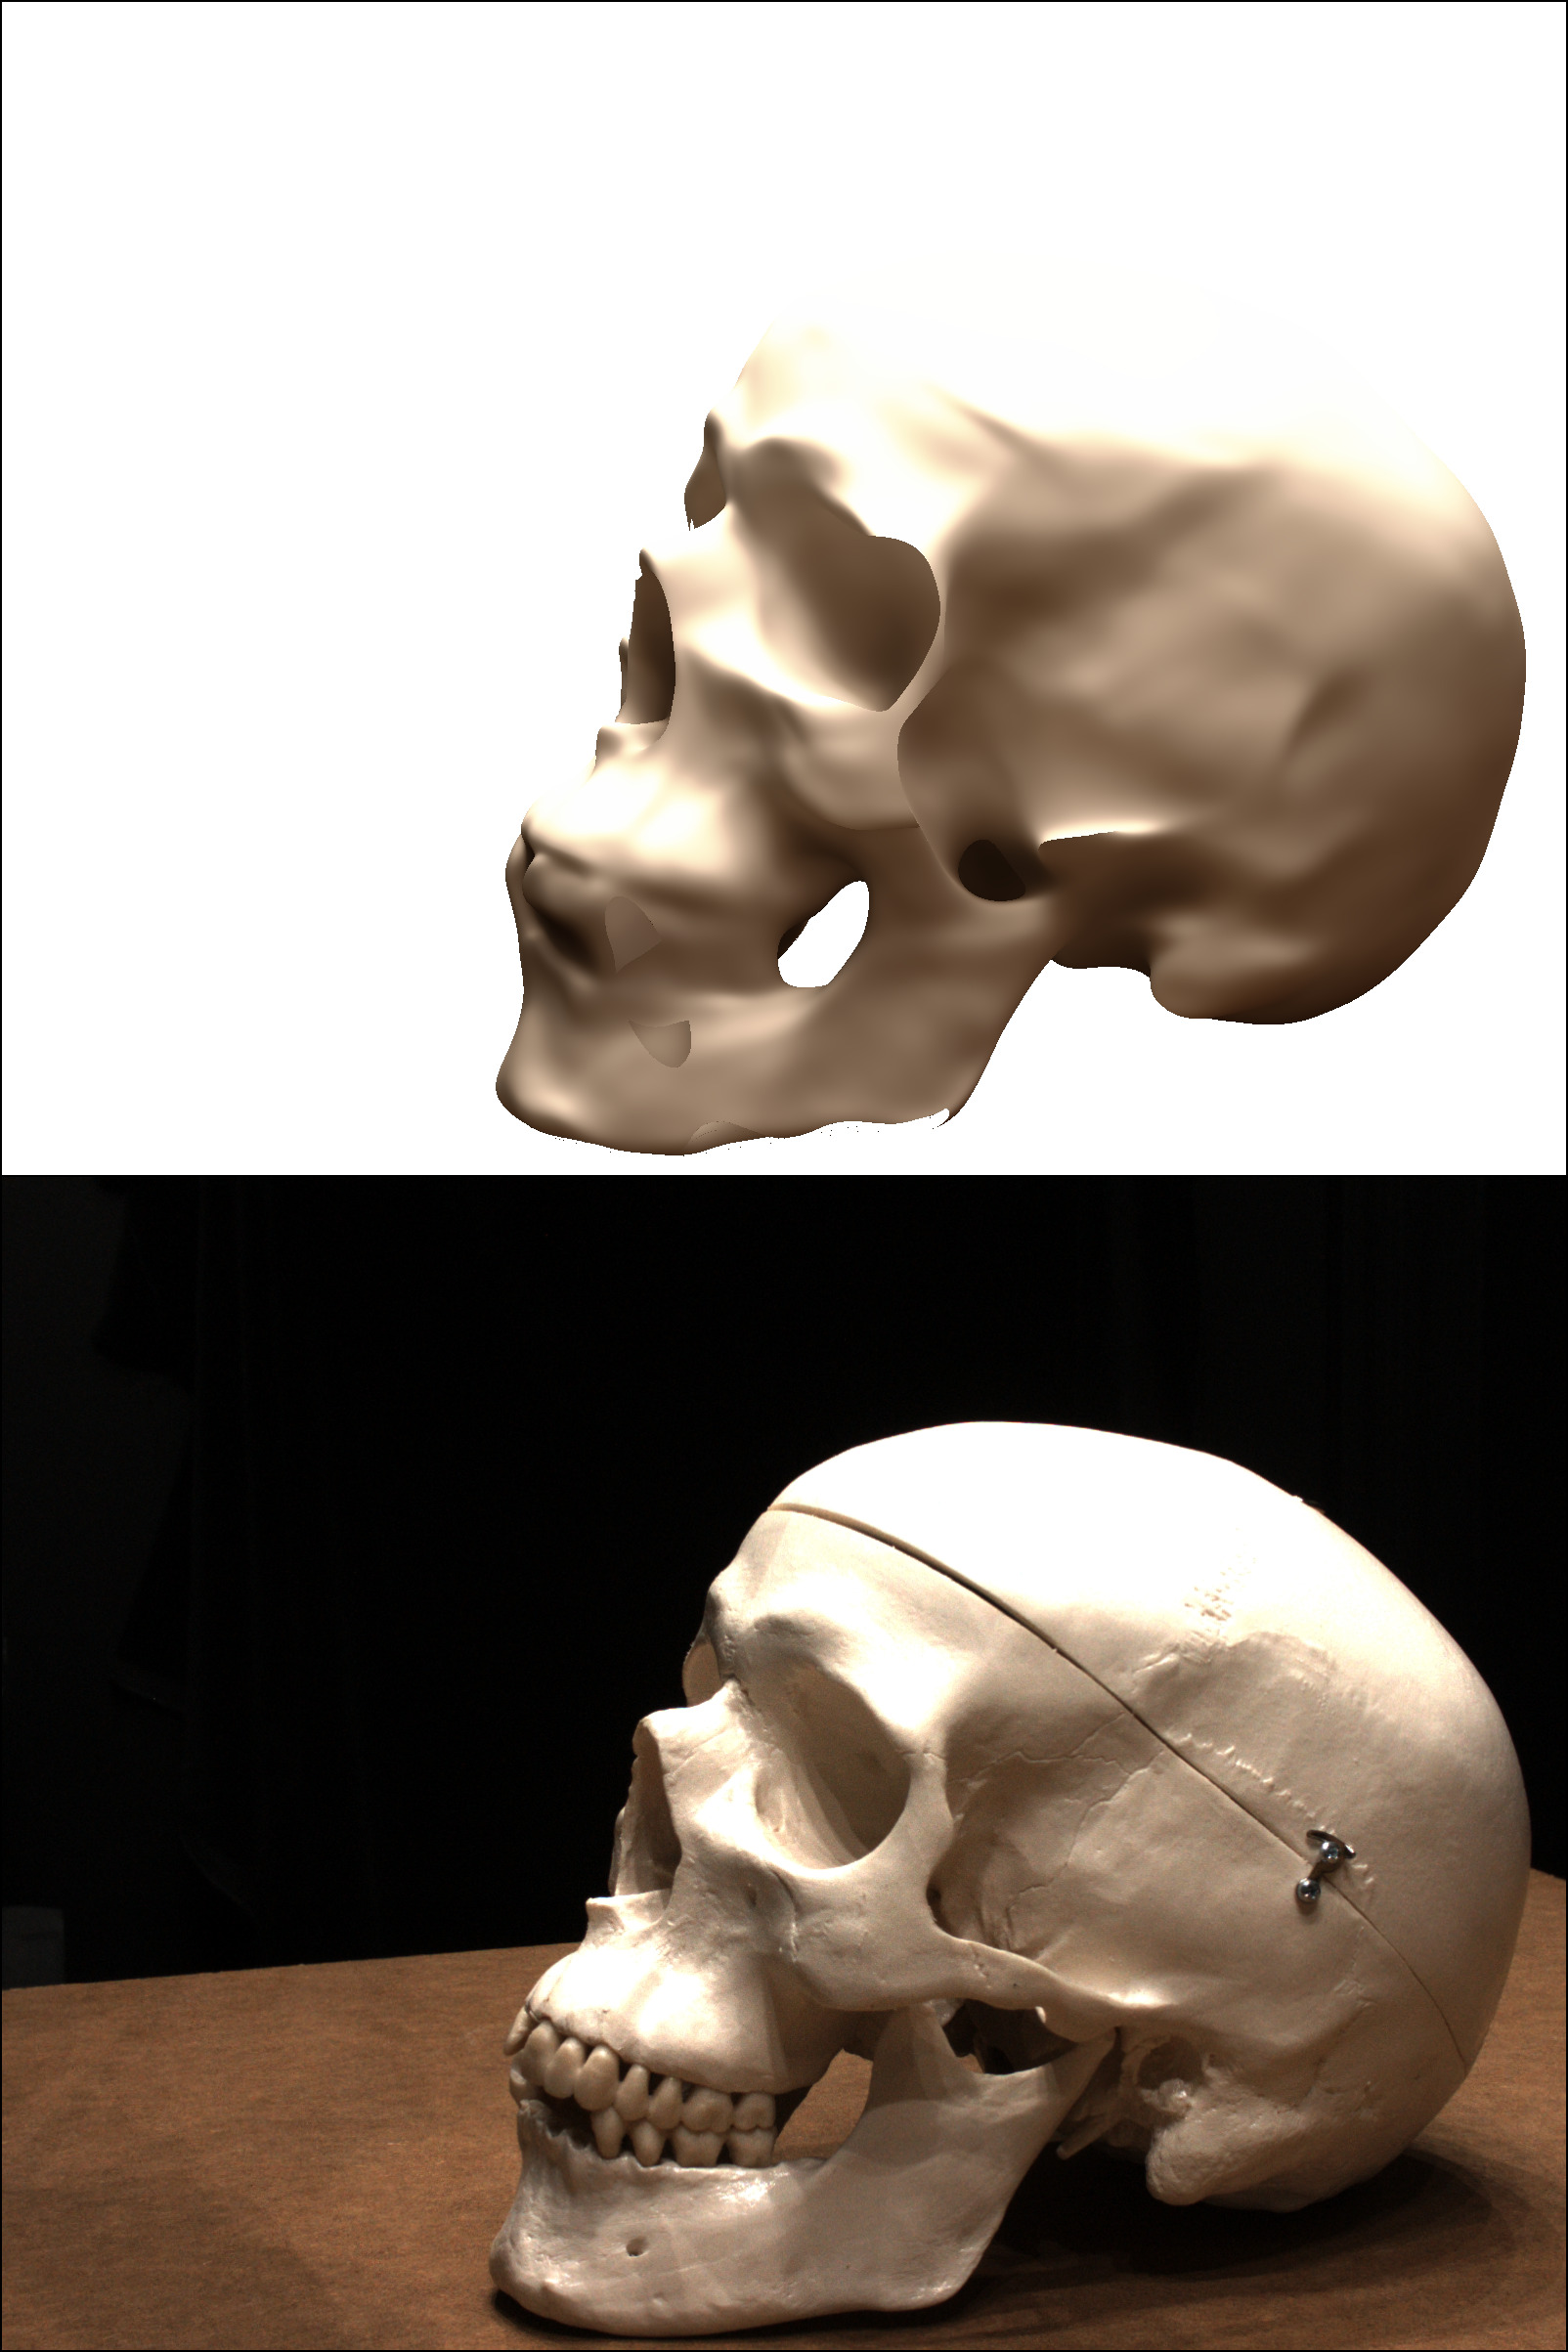
\includegraphics[width=1.5cm]{images/chapter5_img/RenderedImages-DepthMaps-EpochWise-Evals/PositionalEncoding/65/rendering_100.jpg} & 
    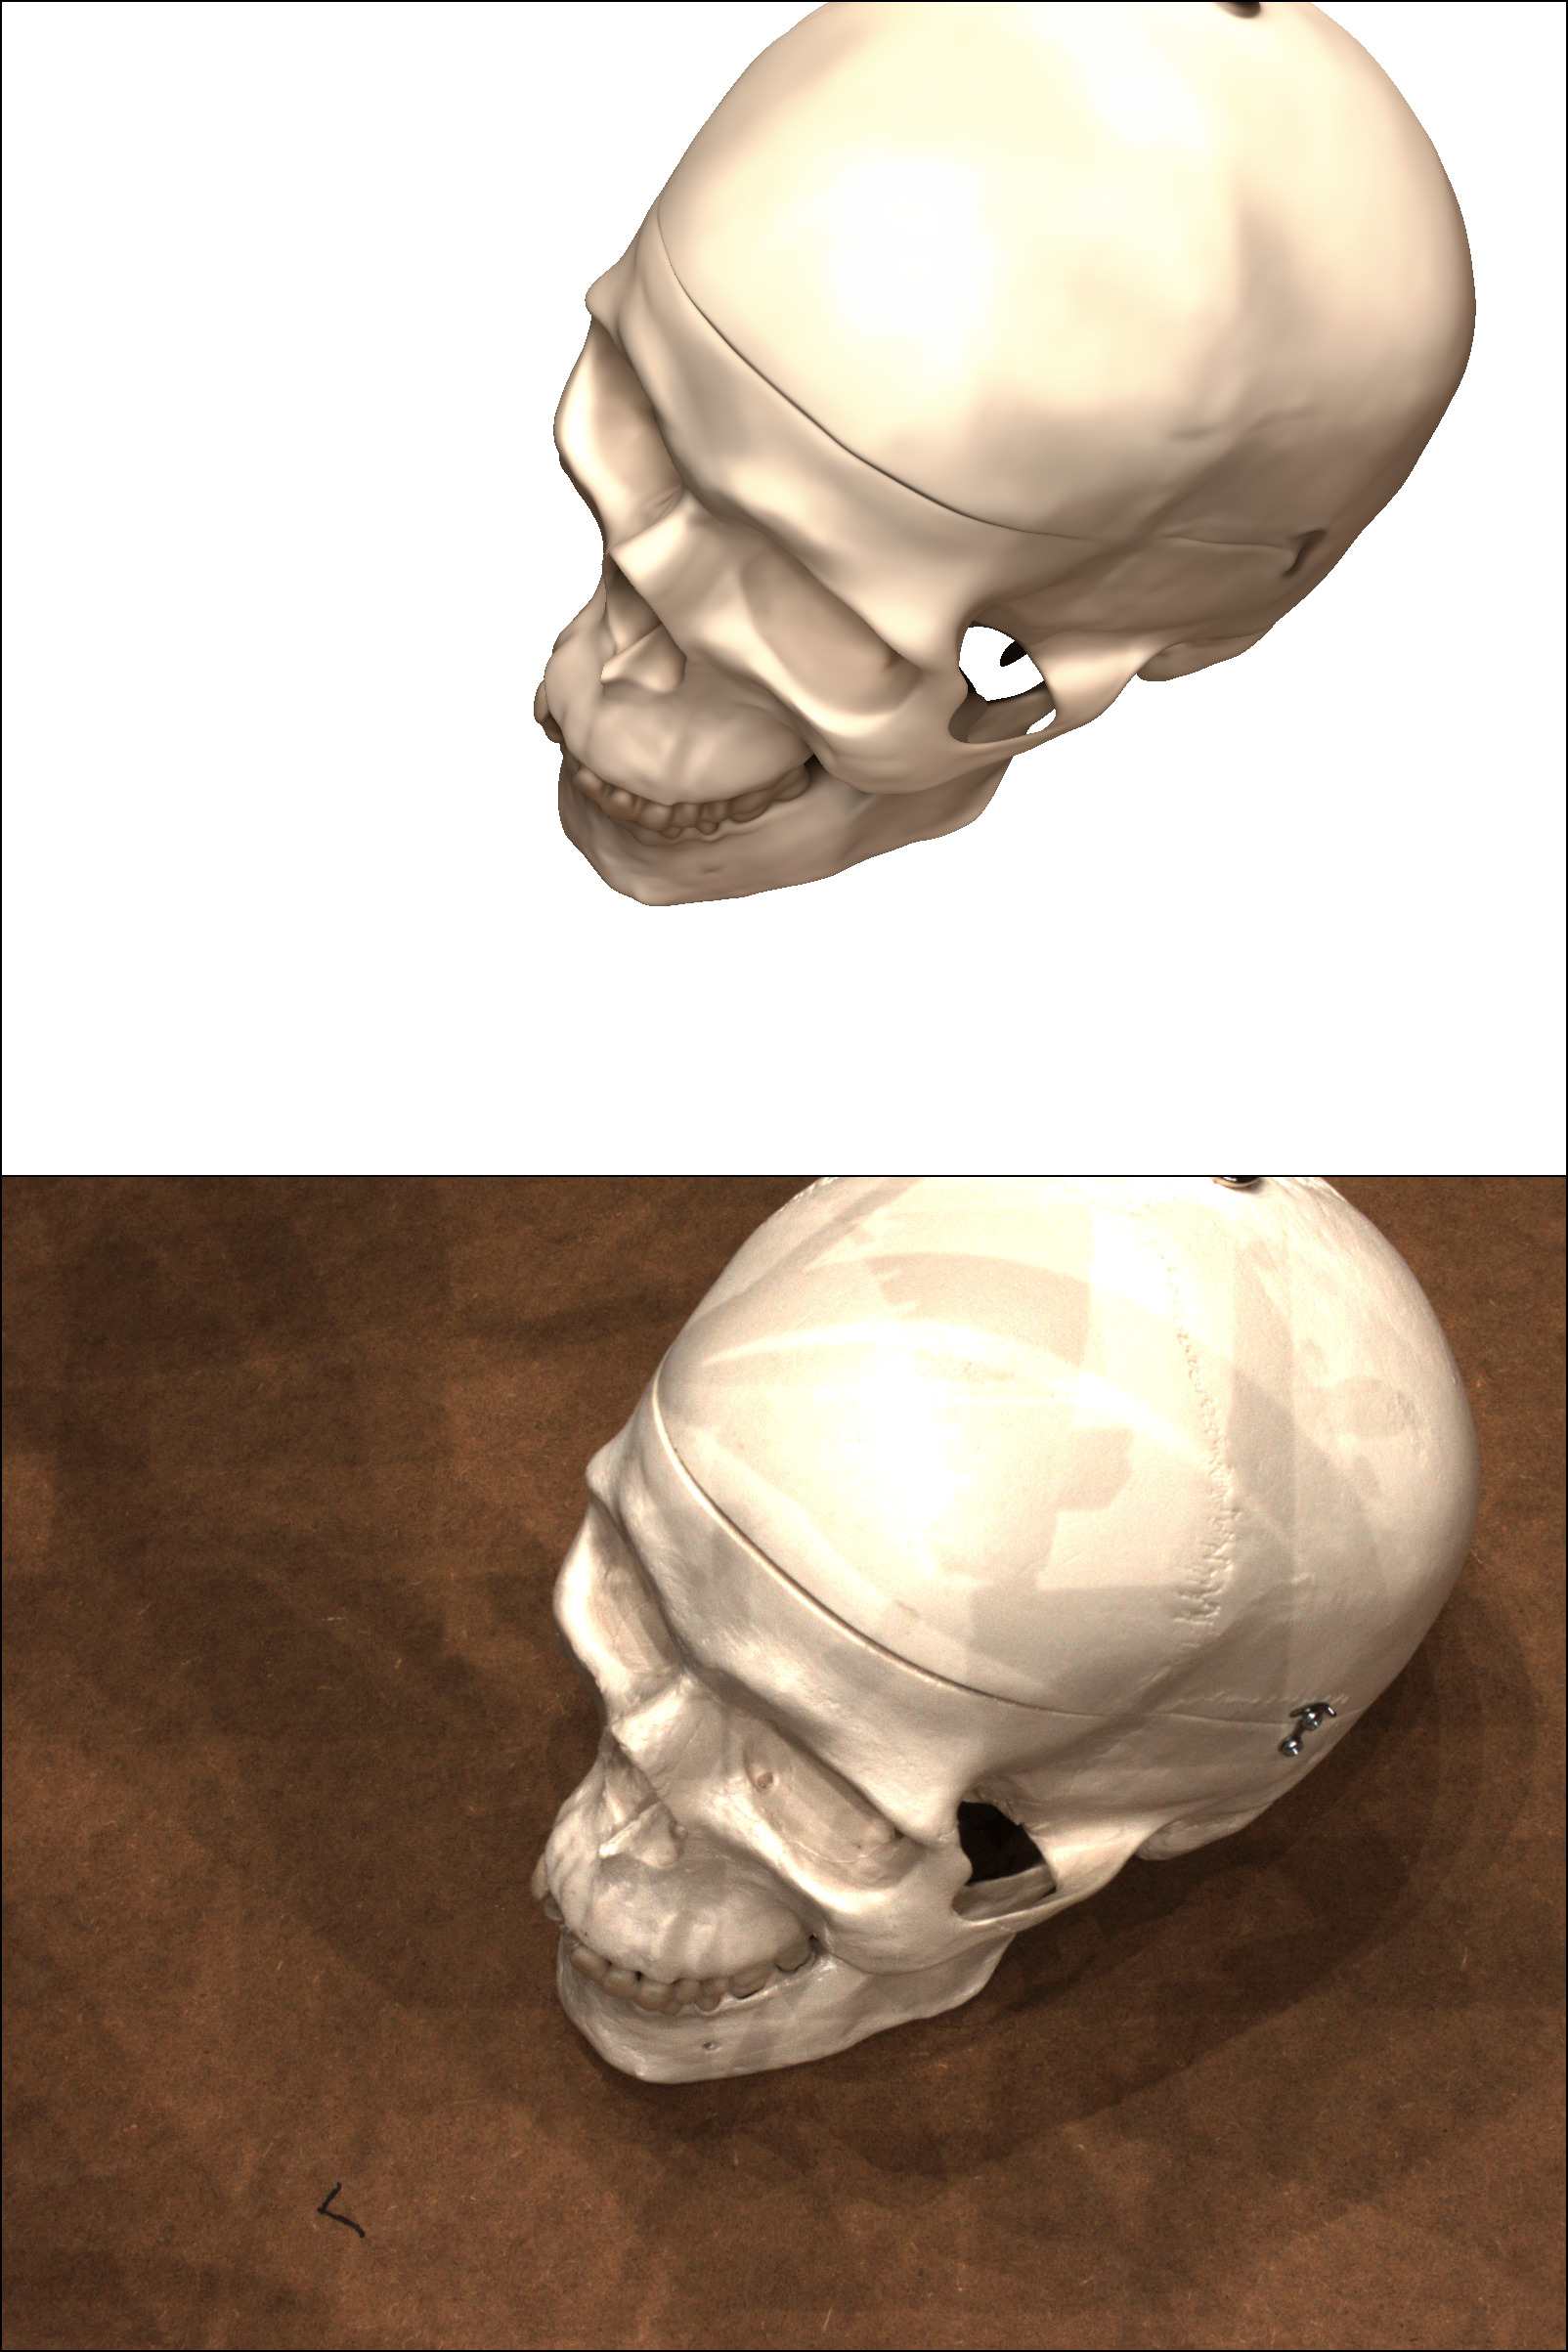
\includegraphics[width=1.5cm]{images/chapter5_img/RenderedImages-DepthMaps-EpochWise-Evals/PositionalEncoding/65/rendering_500.jpg} & 
    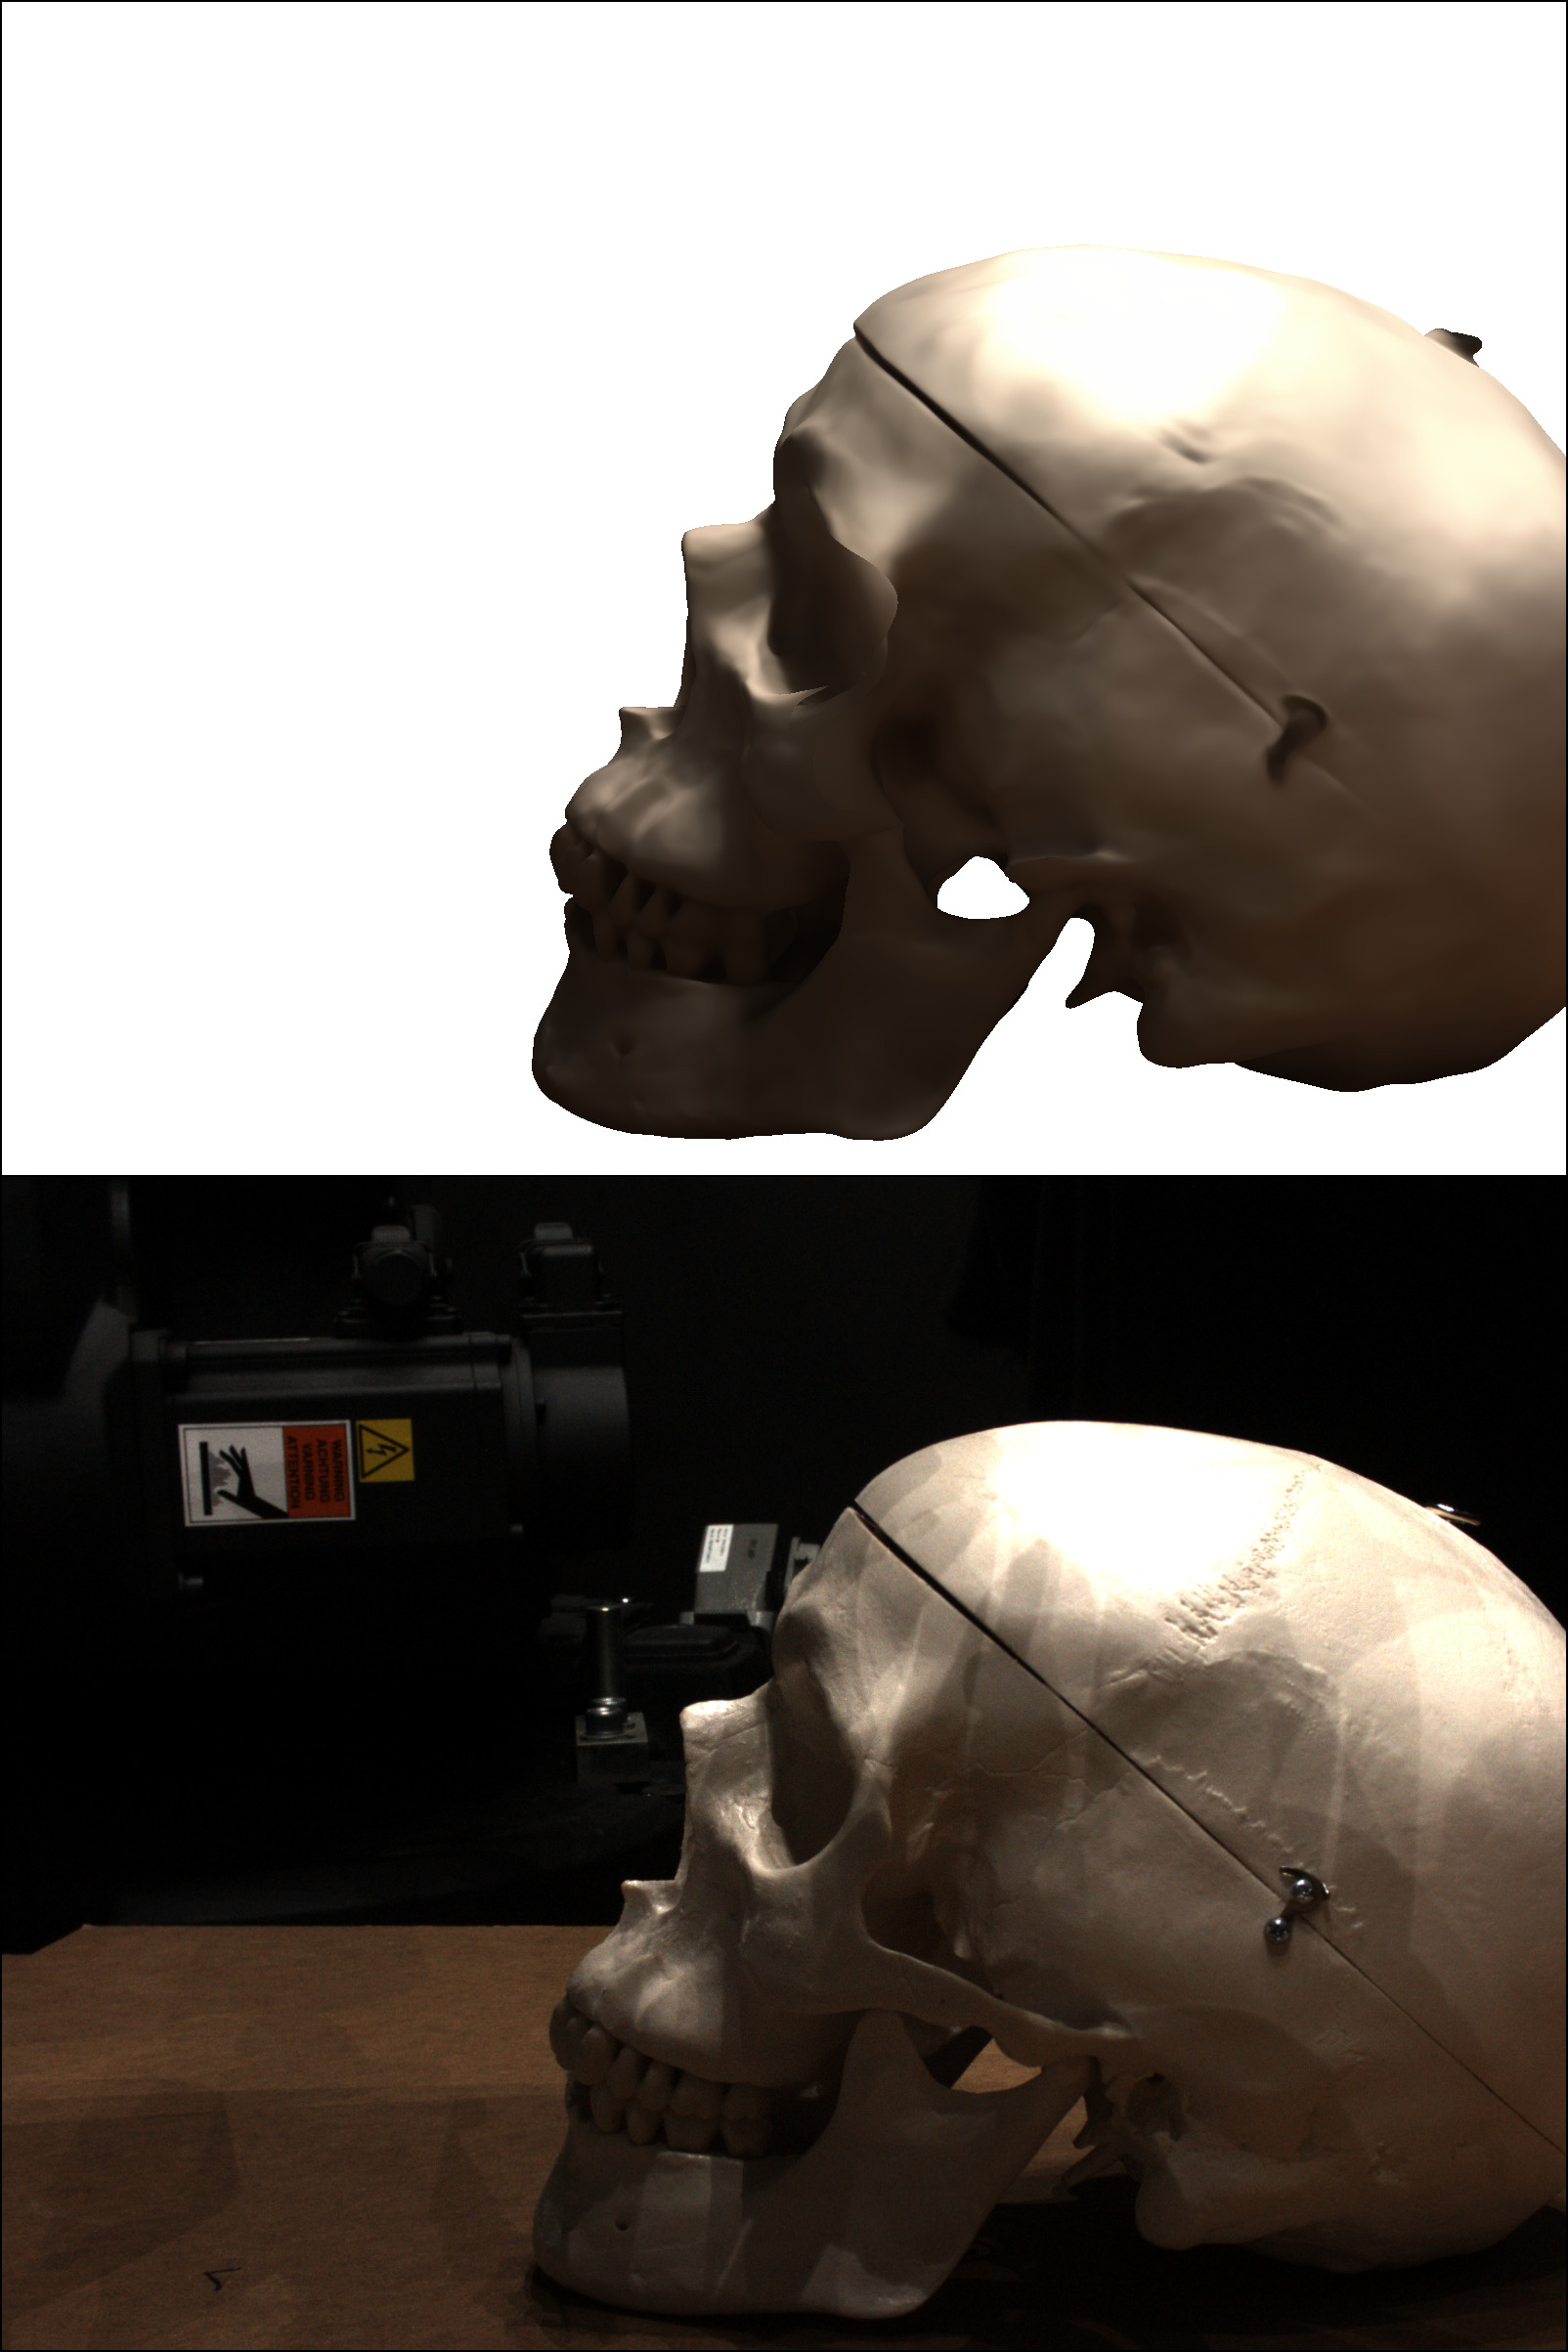
\includegraphics[width=1.5cm]{images/chapter5_img/RenderedImages-DepthMaps-EpochWise-Evals/PositionalEncoding/65/rendering_1000.jpg} & 
    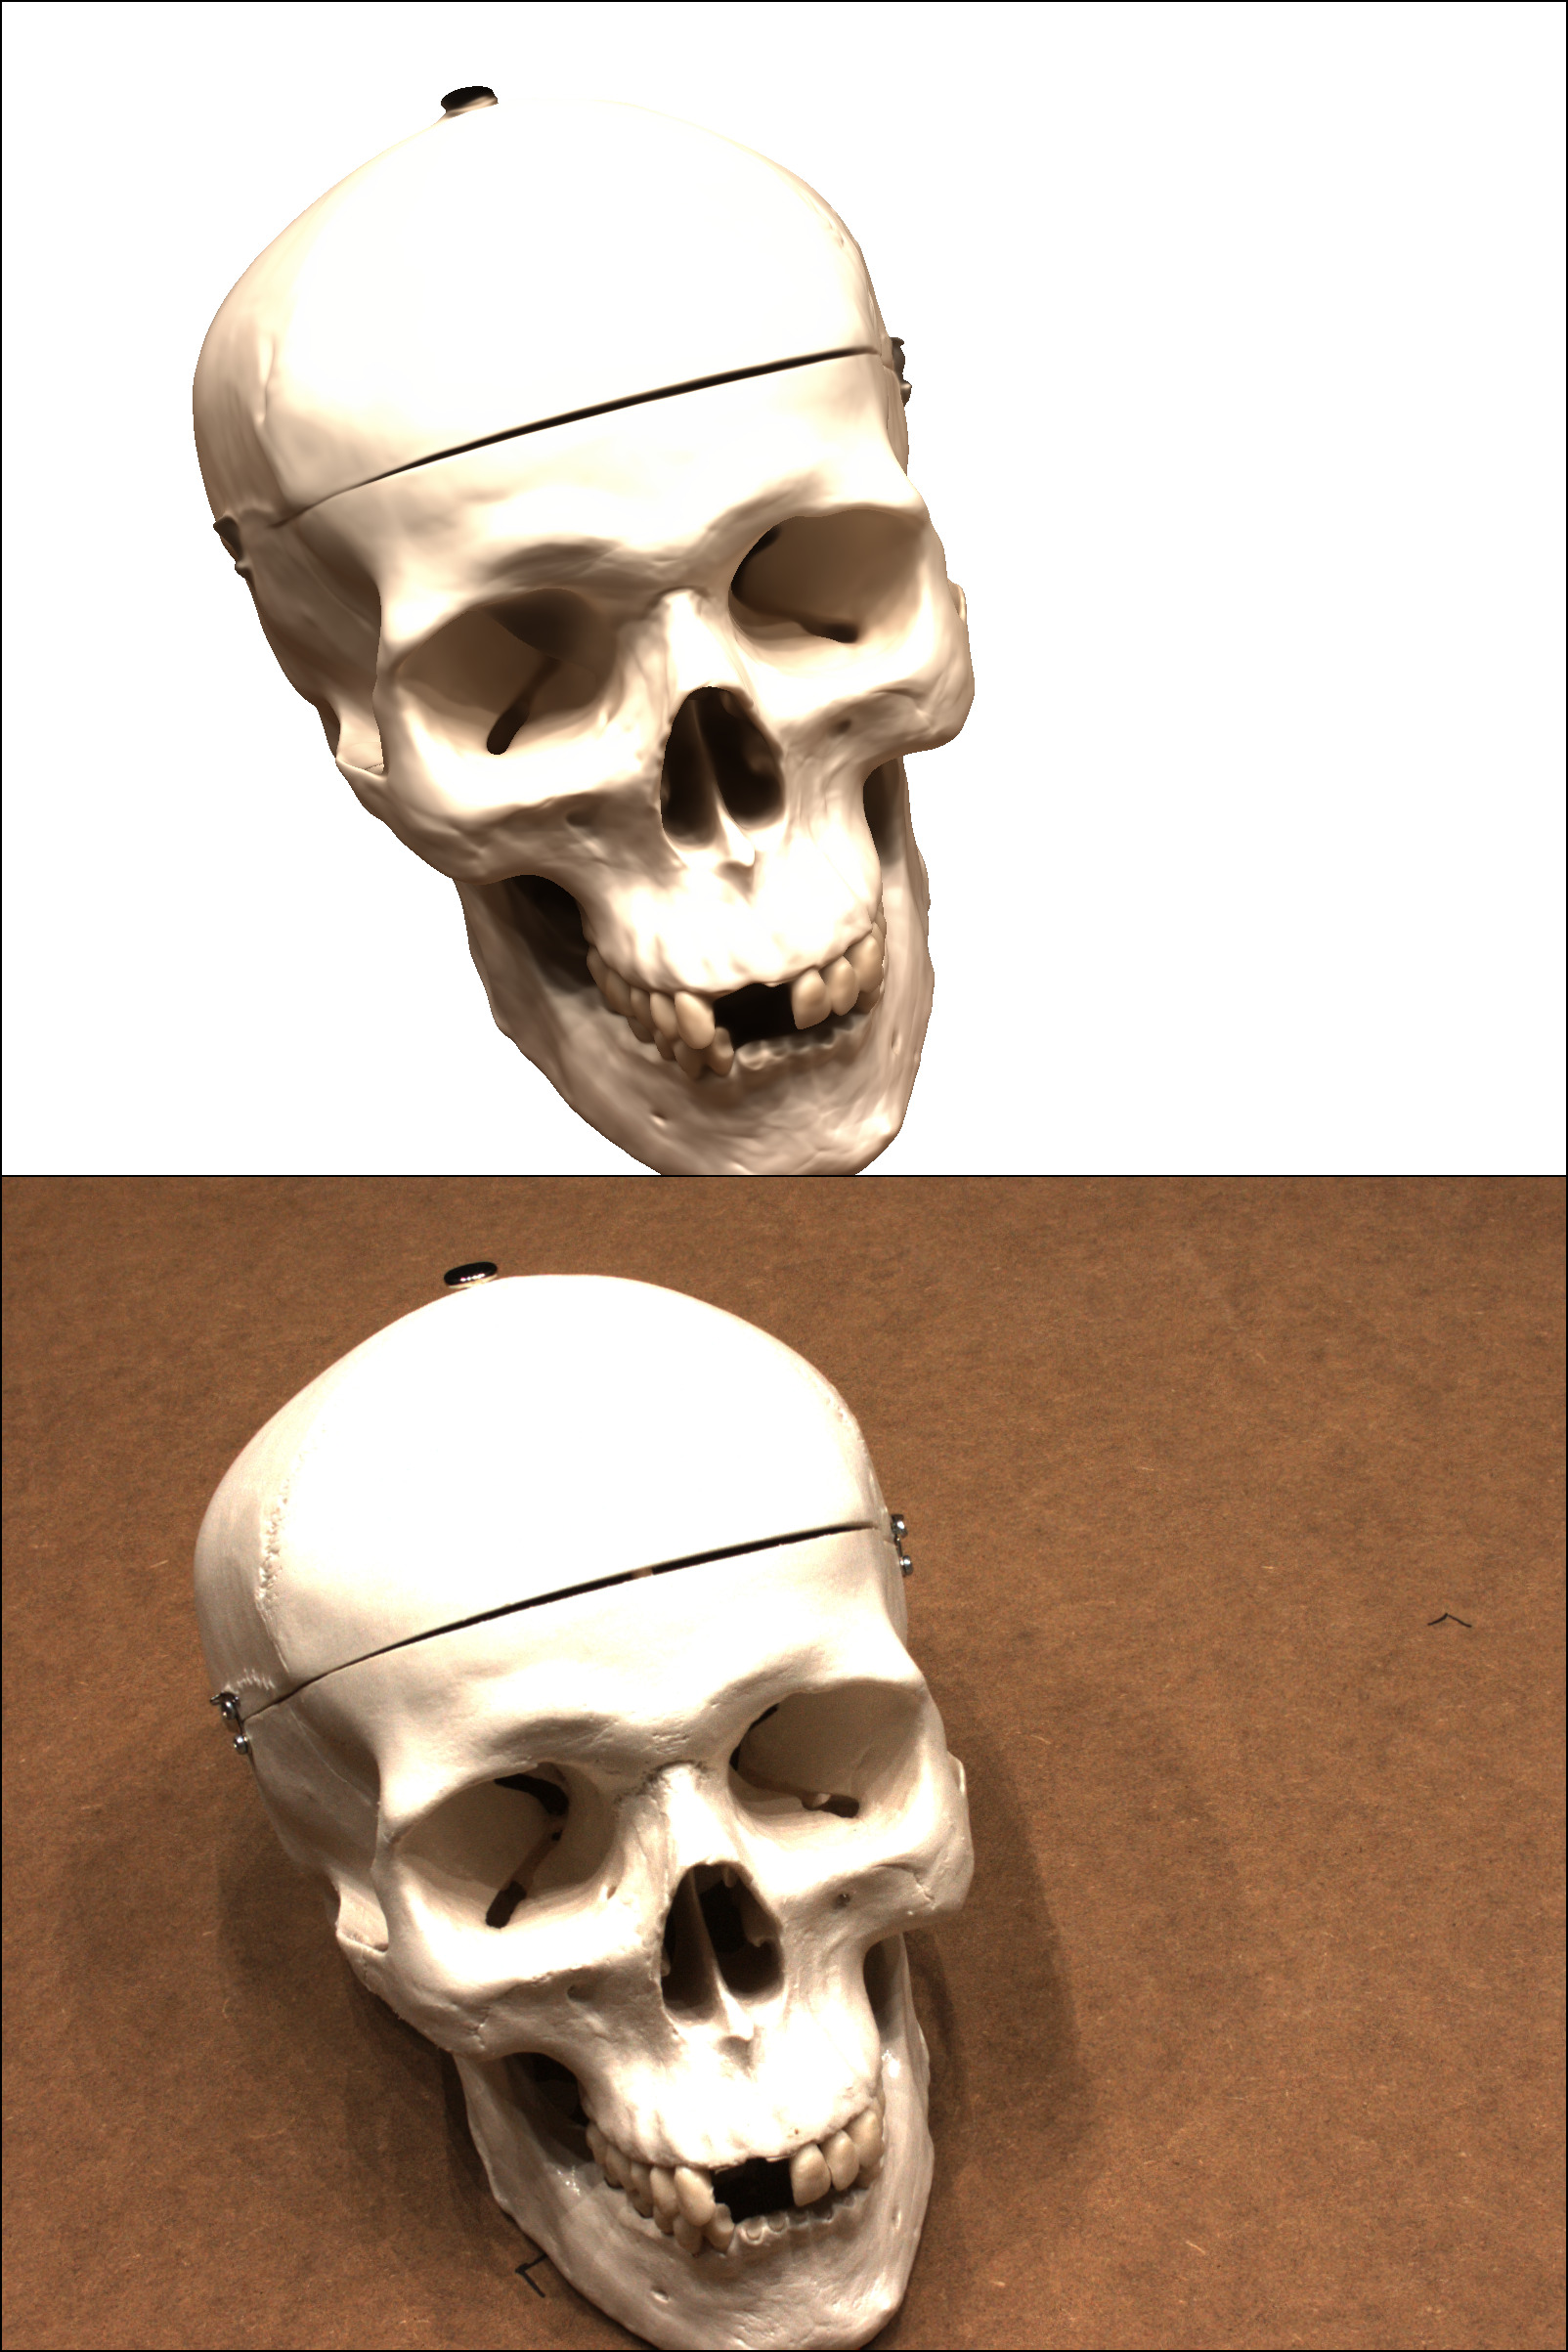
\includegraphics[width=1.5cm]{images/chapter5_img/RenderedImages-DepthMaps-EpochWise-Evals/PositionalEncoding/65/rendering_2000.jpg} & 
    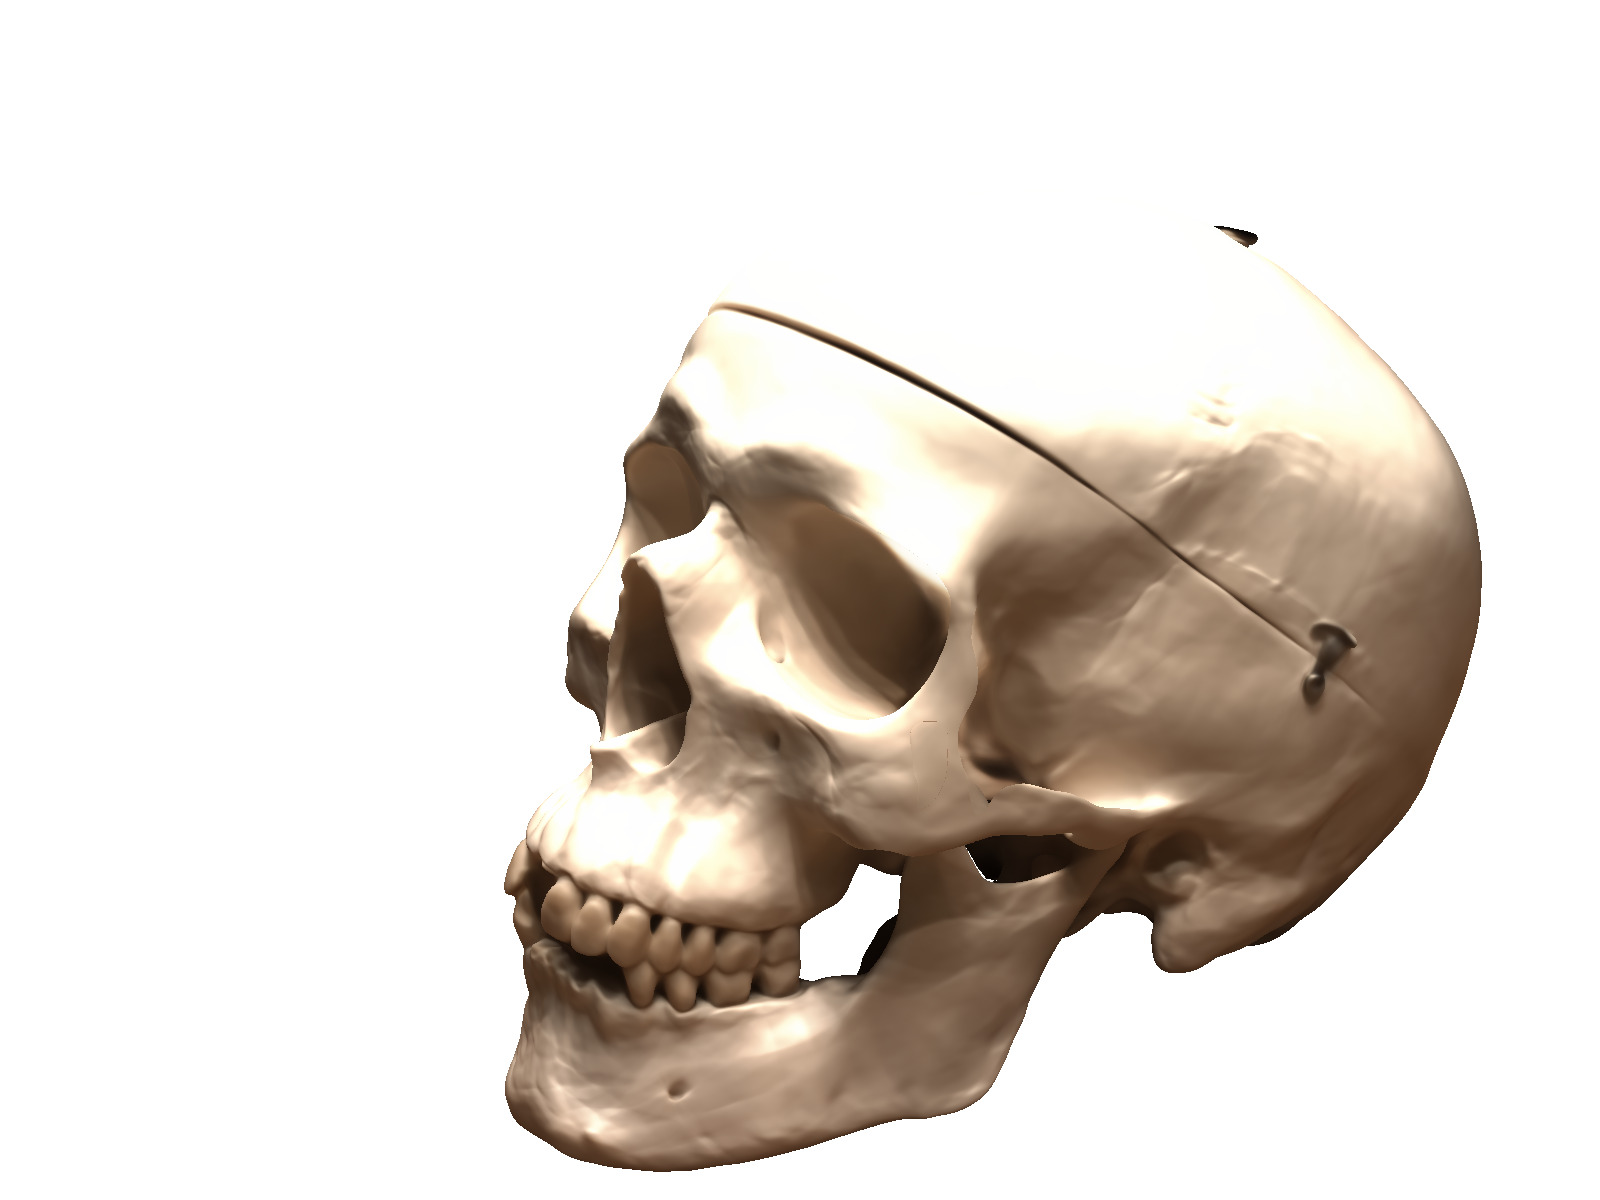
\includegraphics[width=1.5cm]{images/chapter5_img/RenderedImages-DepthMaps-EpochWise-Evals/PositionalEncoding/65/eval_035.jpg} \\
    \hline
    FourierNTK & 
    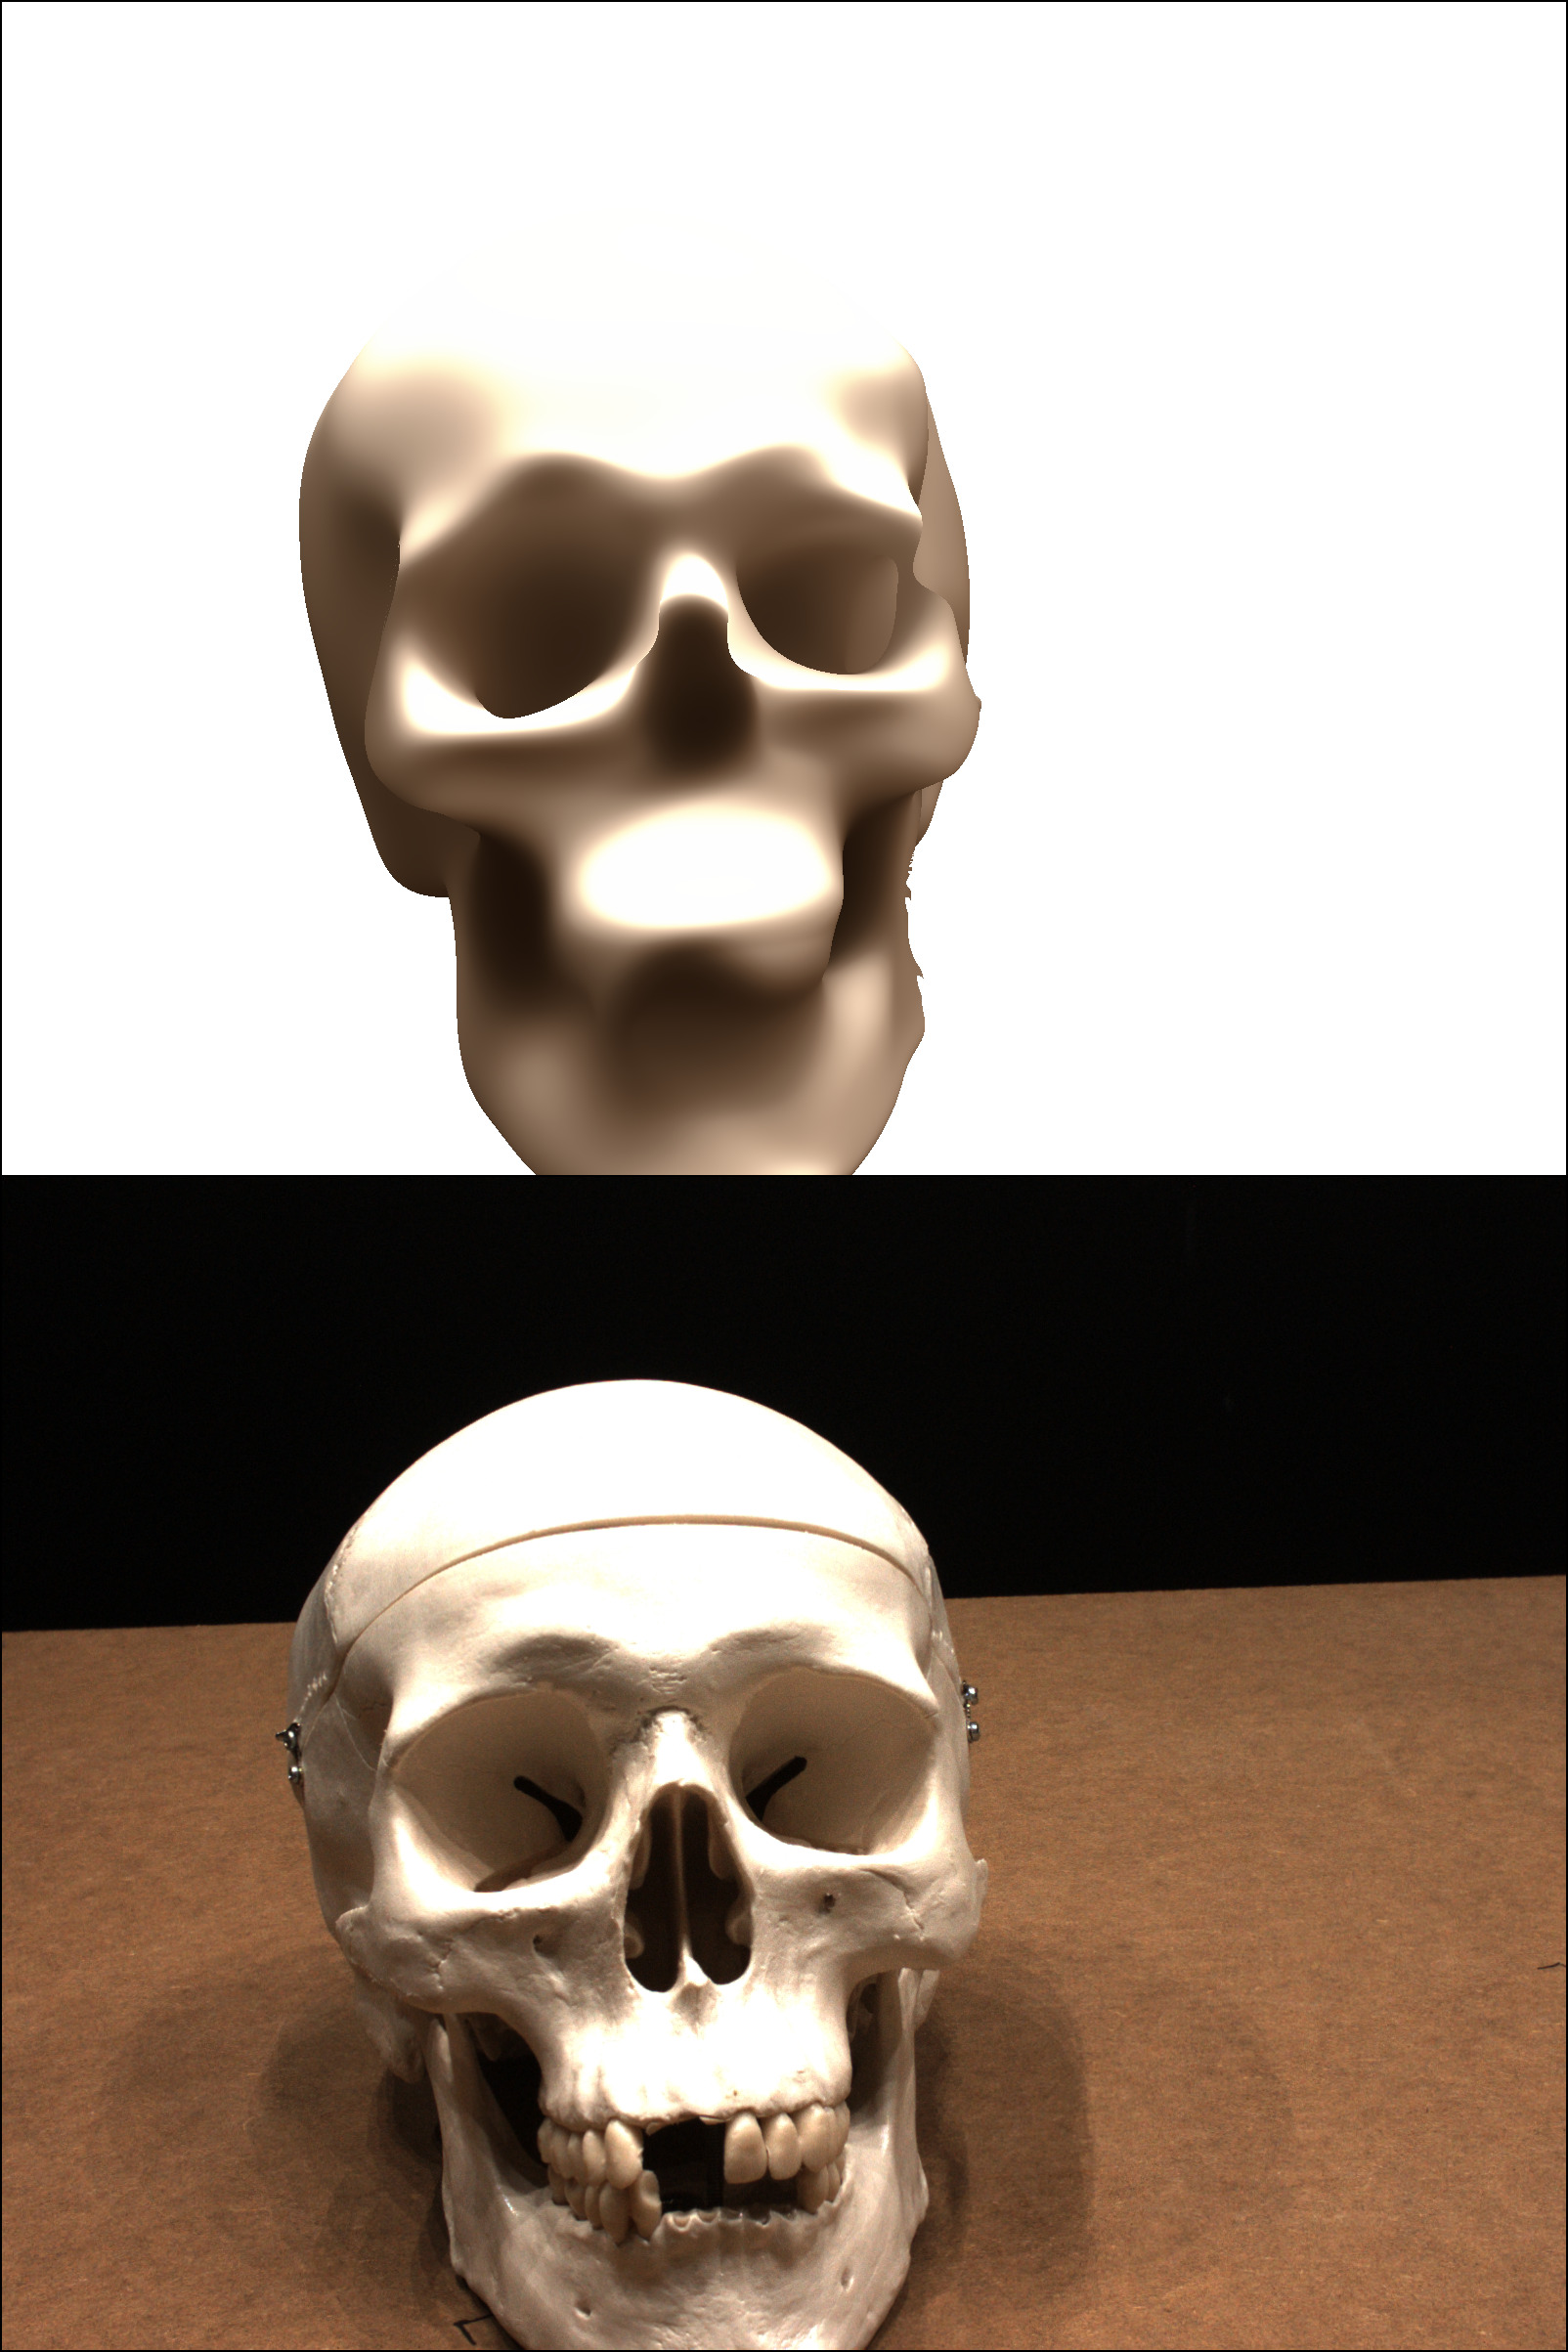
\includegraphics[width=1.5cm]{images/chapter5_img/RenderedImages-DepthMaps-EpochWise-Evals/FourierNTK/65/rendering_100.jpg} & 
    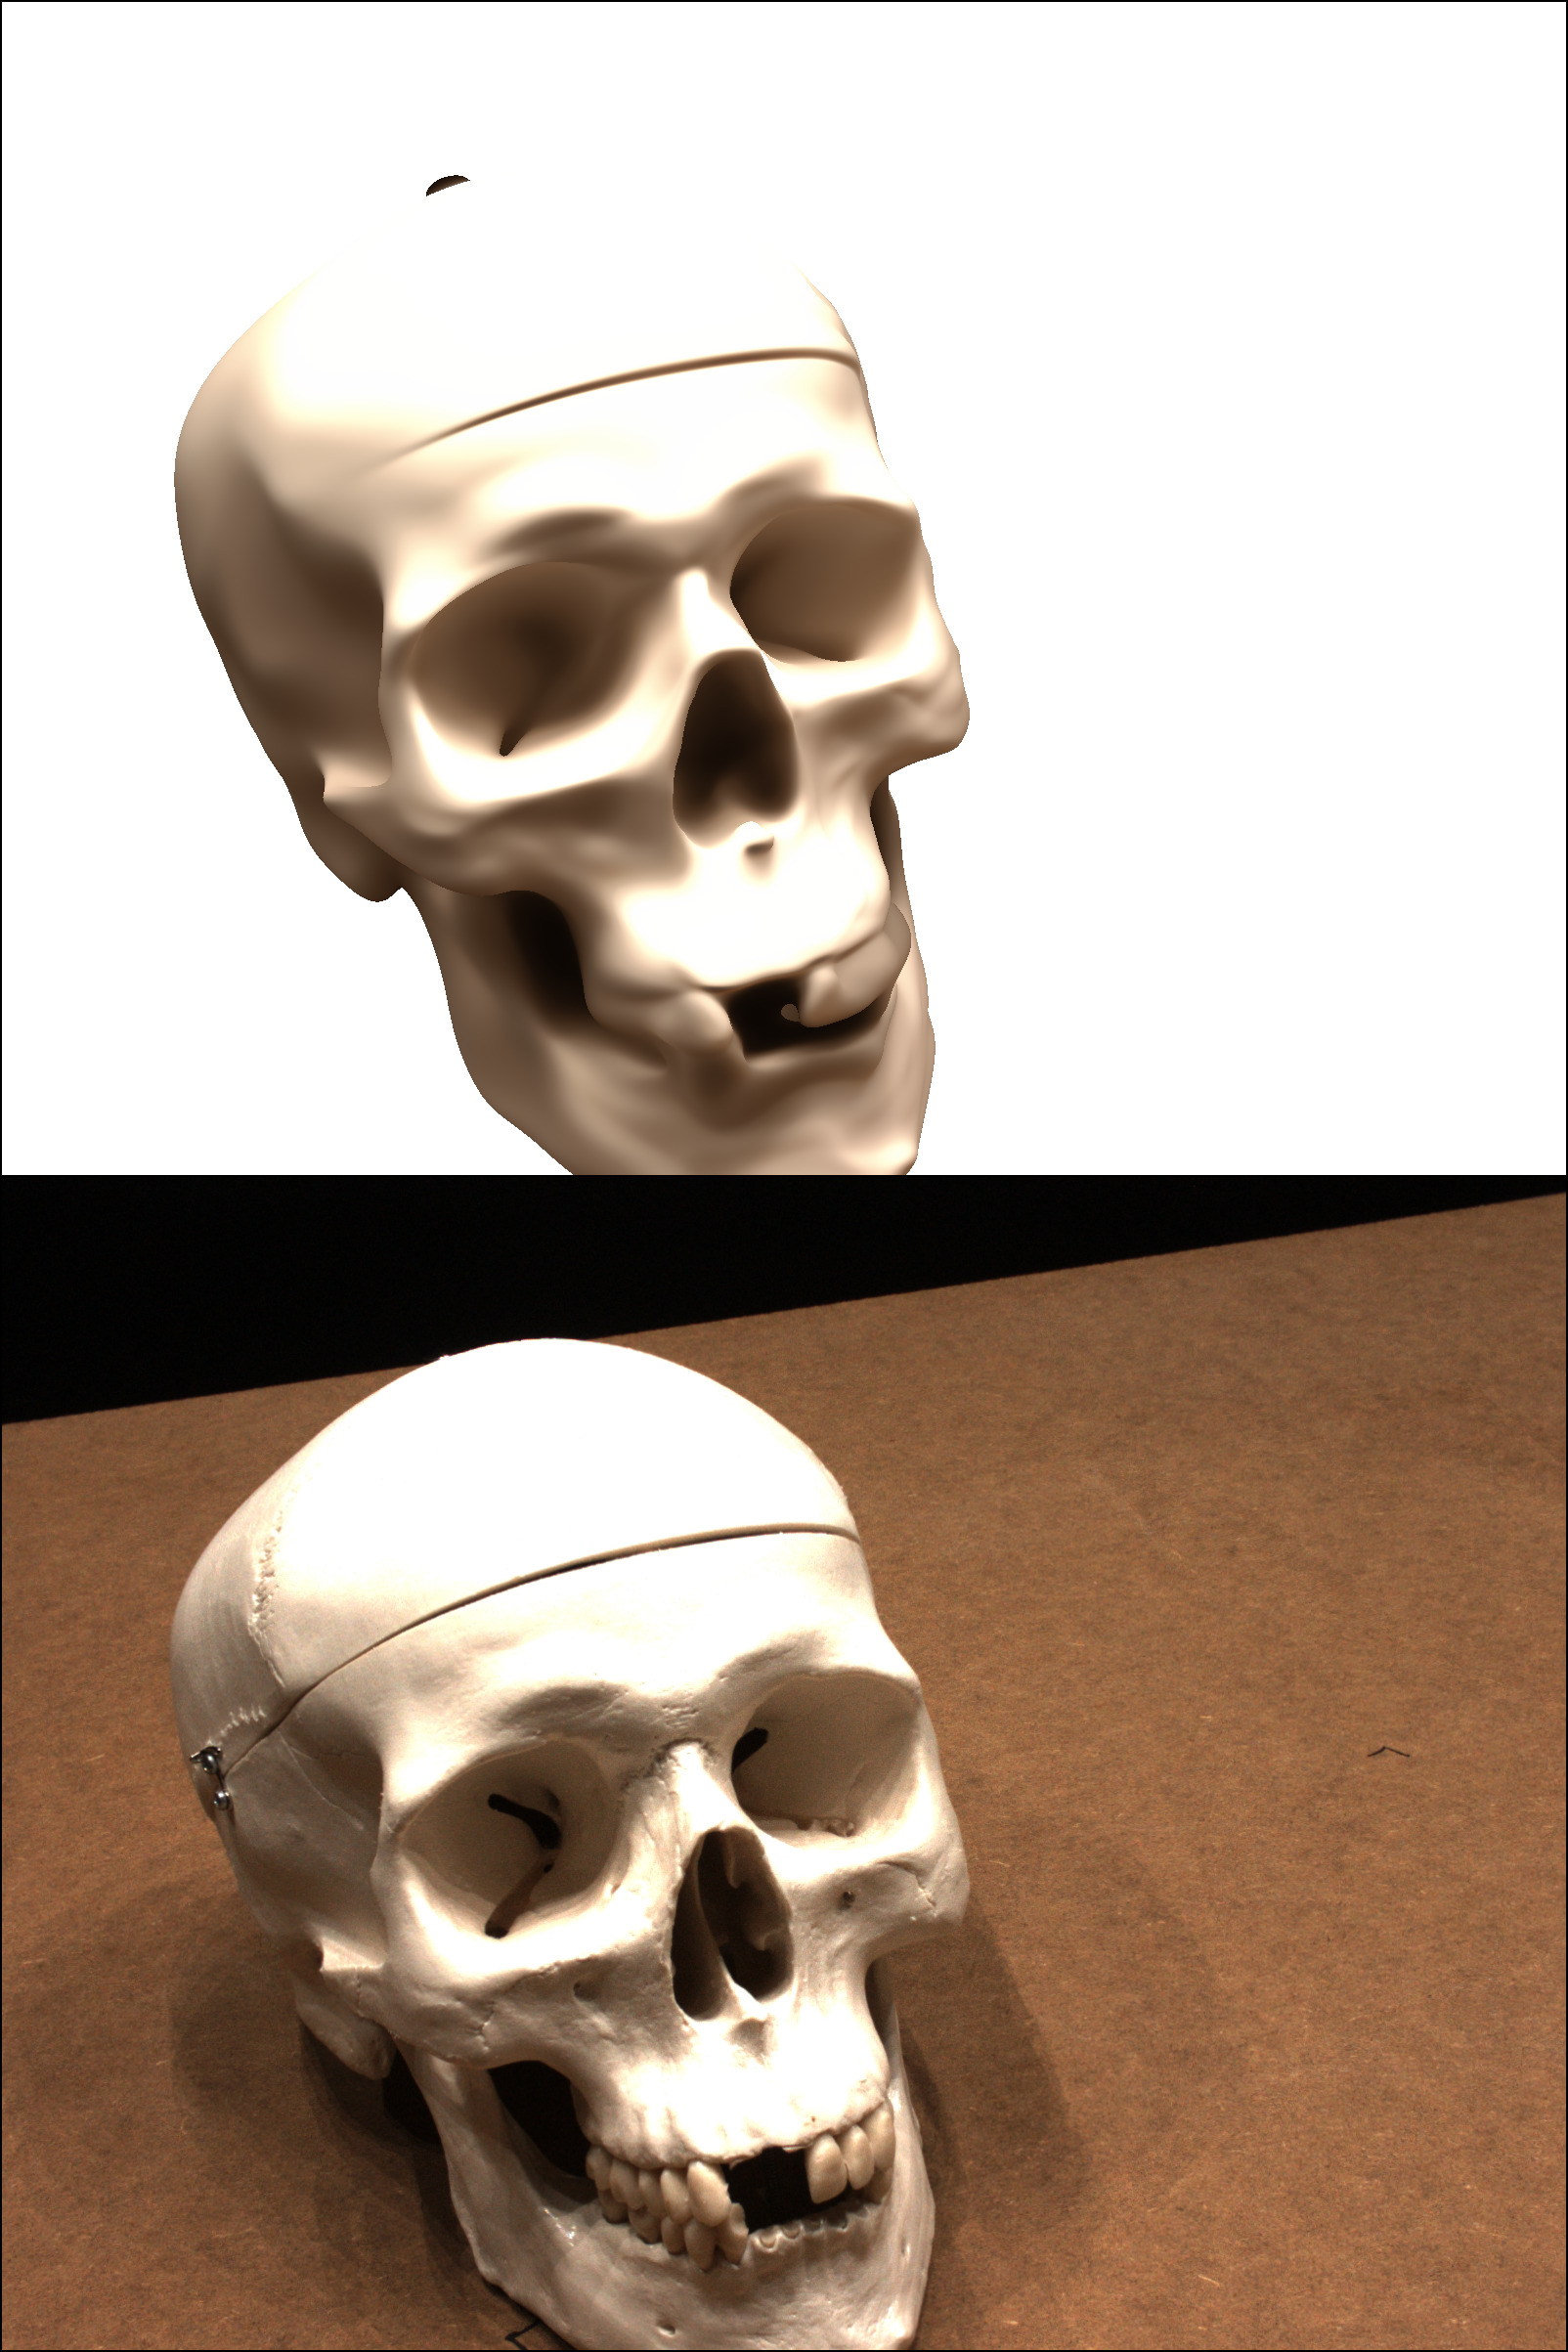
\includegraphics[width=1.5cm]{images/chapter5_img/RenderedImages-DepthMaps-EpochWise-Evals/FourierNTK/65/rendering_500.jpg} & 
    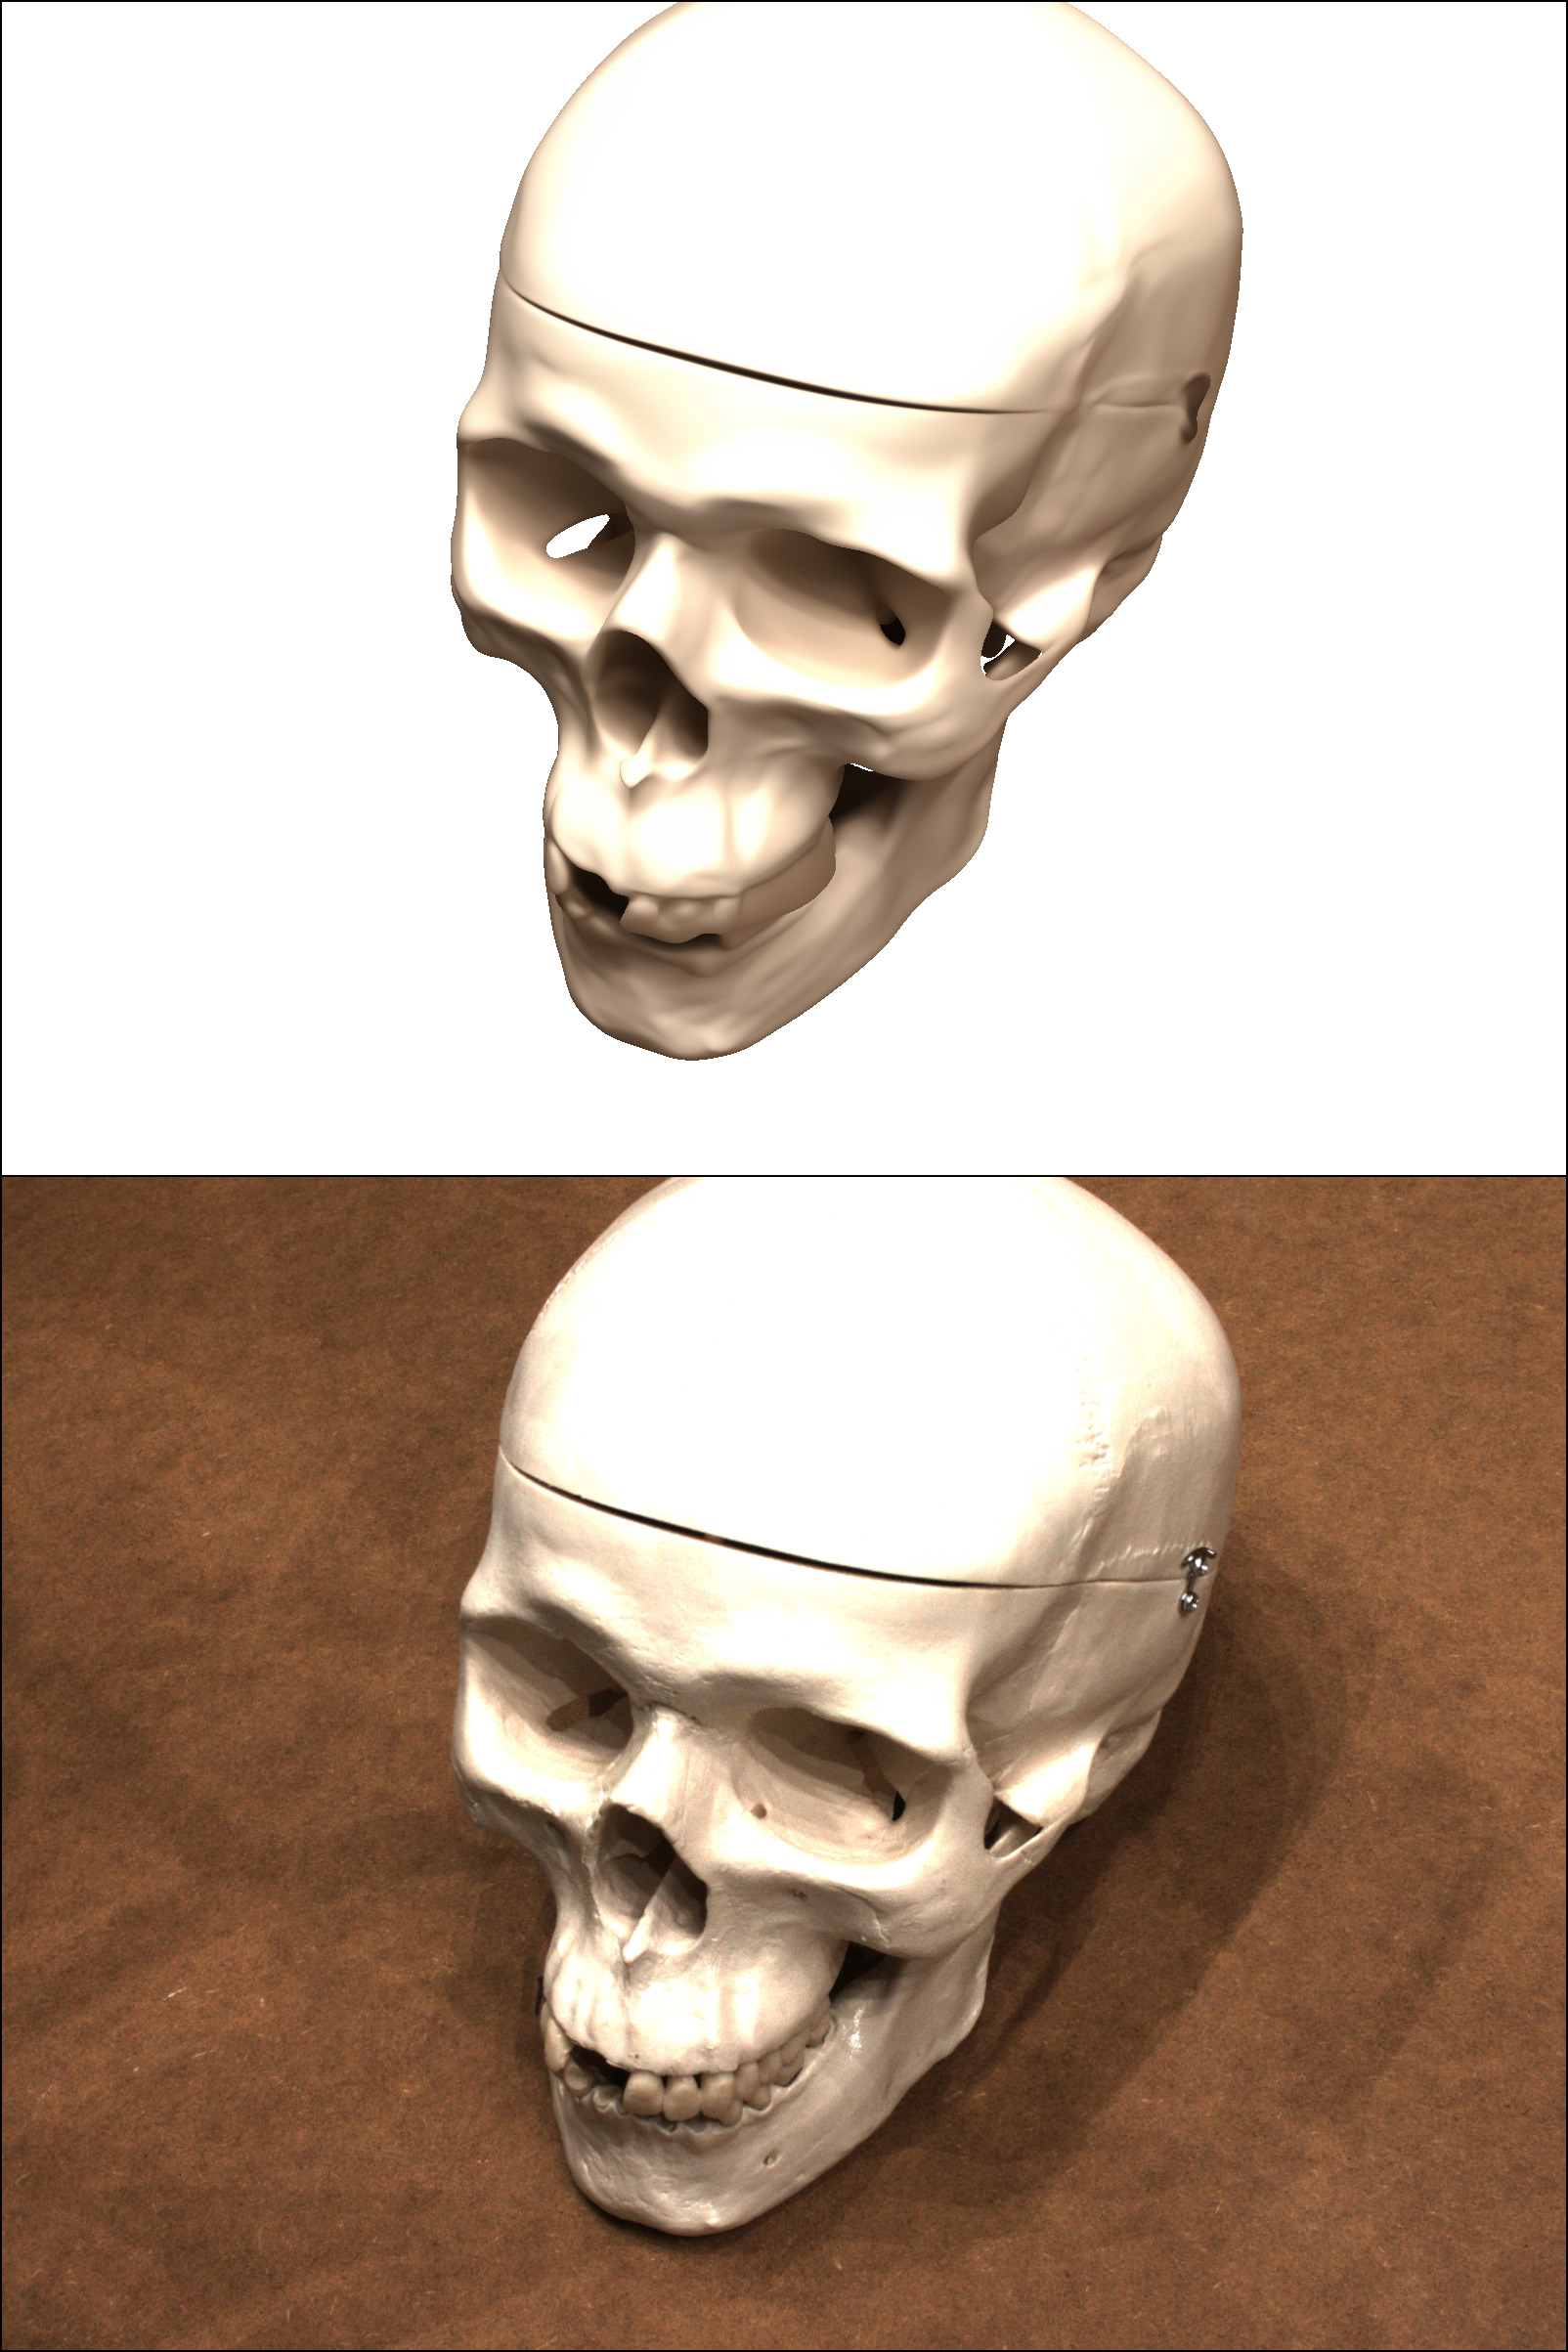
\includegraphics[width=1.5cm]{images/chapter5_img/RenderedImages-DepthMaps-EpochWise-Evals/FourierNTK/65/rendering_1000.jpg} & 
    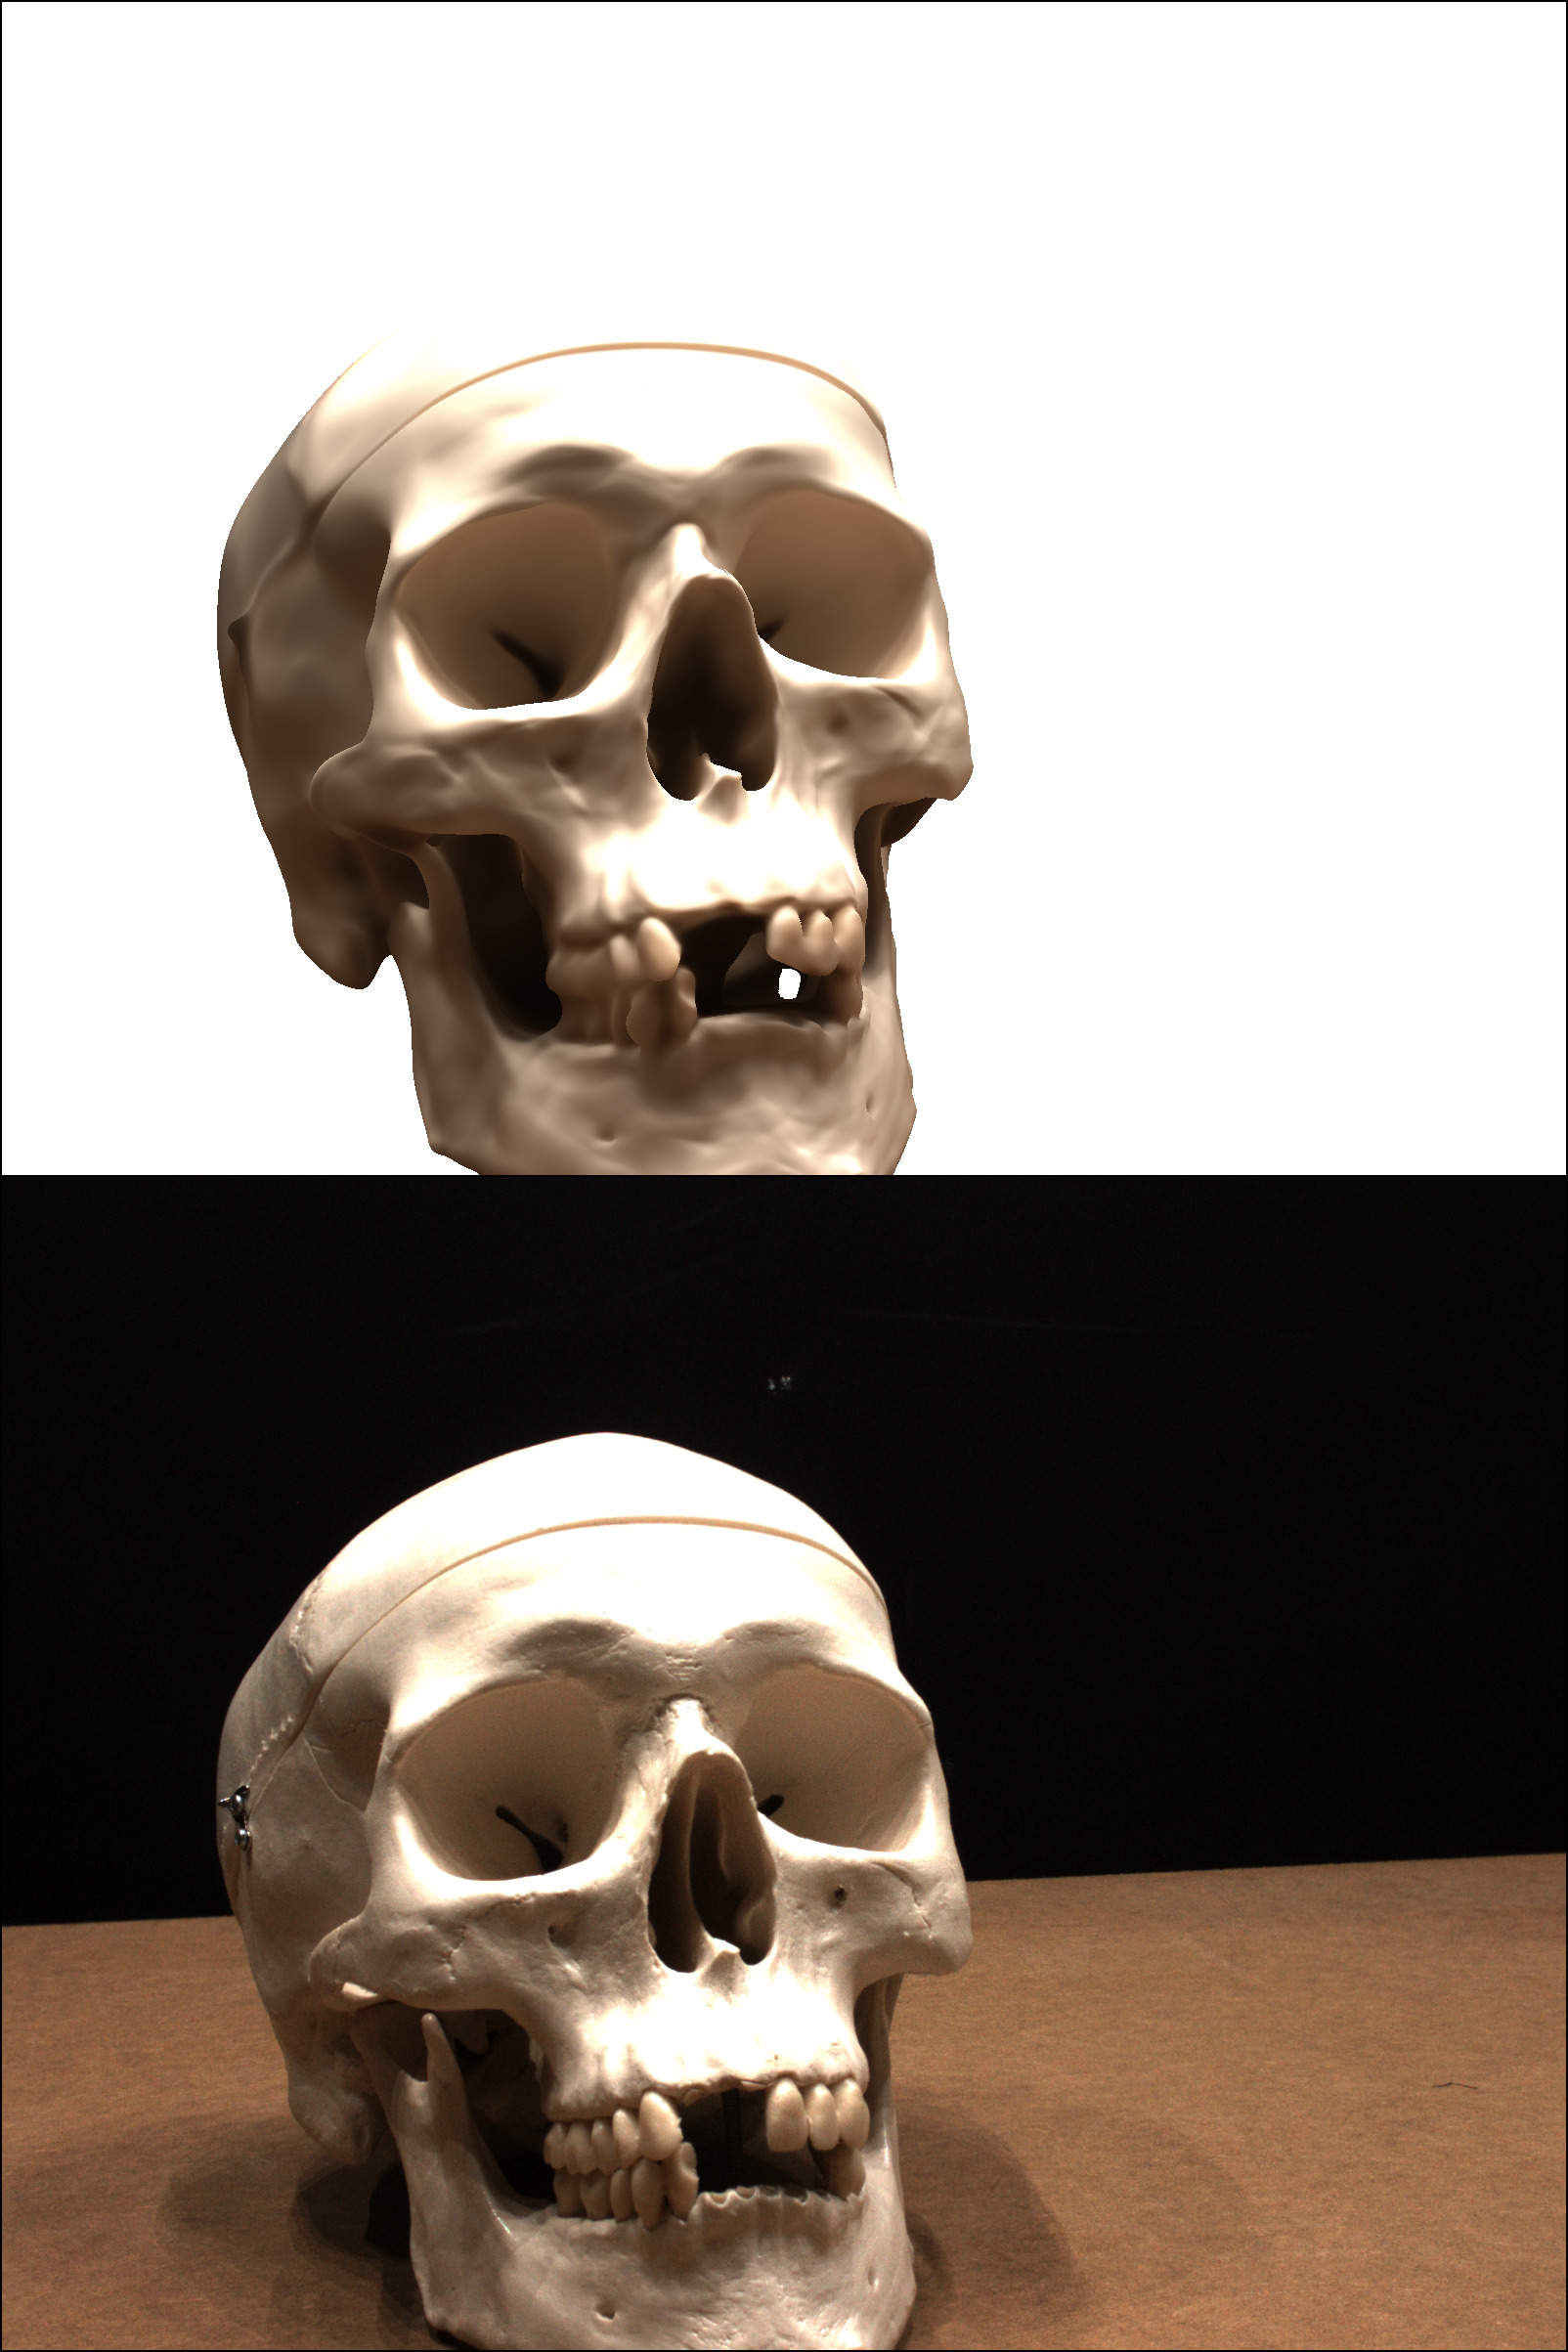
\includegraphics[width=1.5cm]{images/chapter5_img/RenderedImages-DepthMaps-EpochWise-Evals/FourierNTK/65/rendering_2000.jpg} & 
    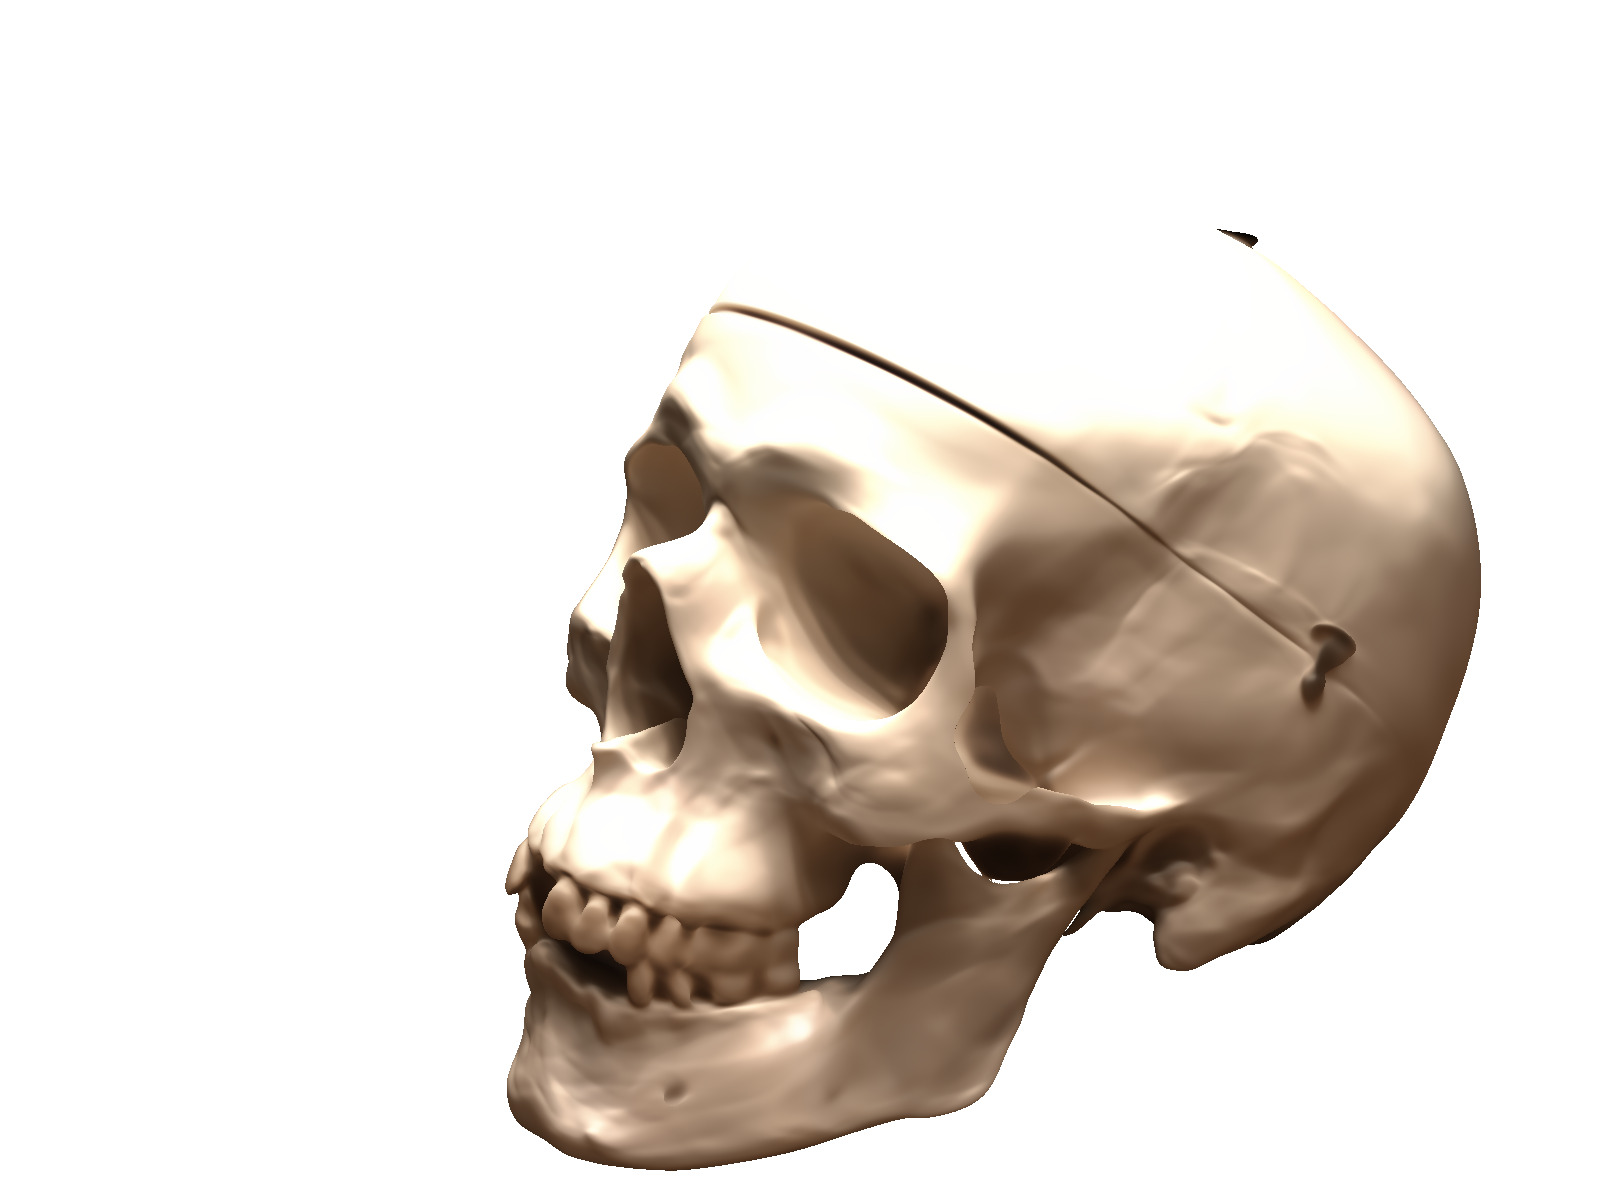
\includegraphics[width=1.5cm]{images/chapter5_img/RenderedImages-DepthMaps-EpochWise-Evals/FourierNTK/65/eval_035.jpg} \\
    \hline
    MR-HashGrid3D & 
    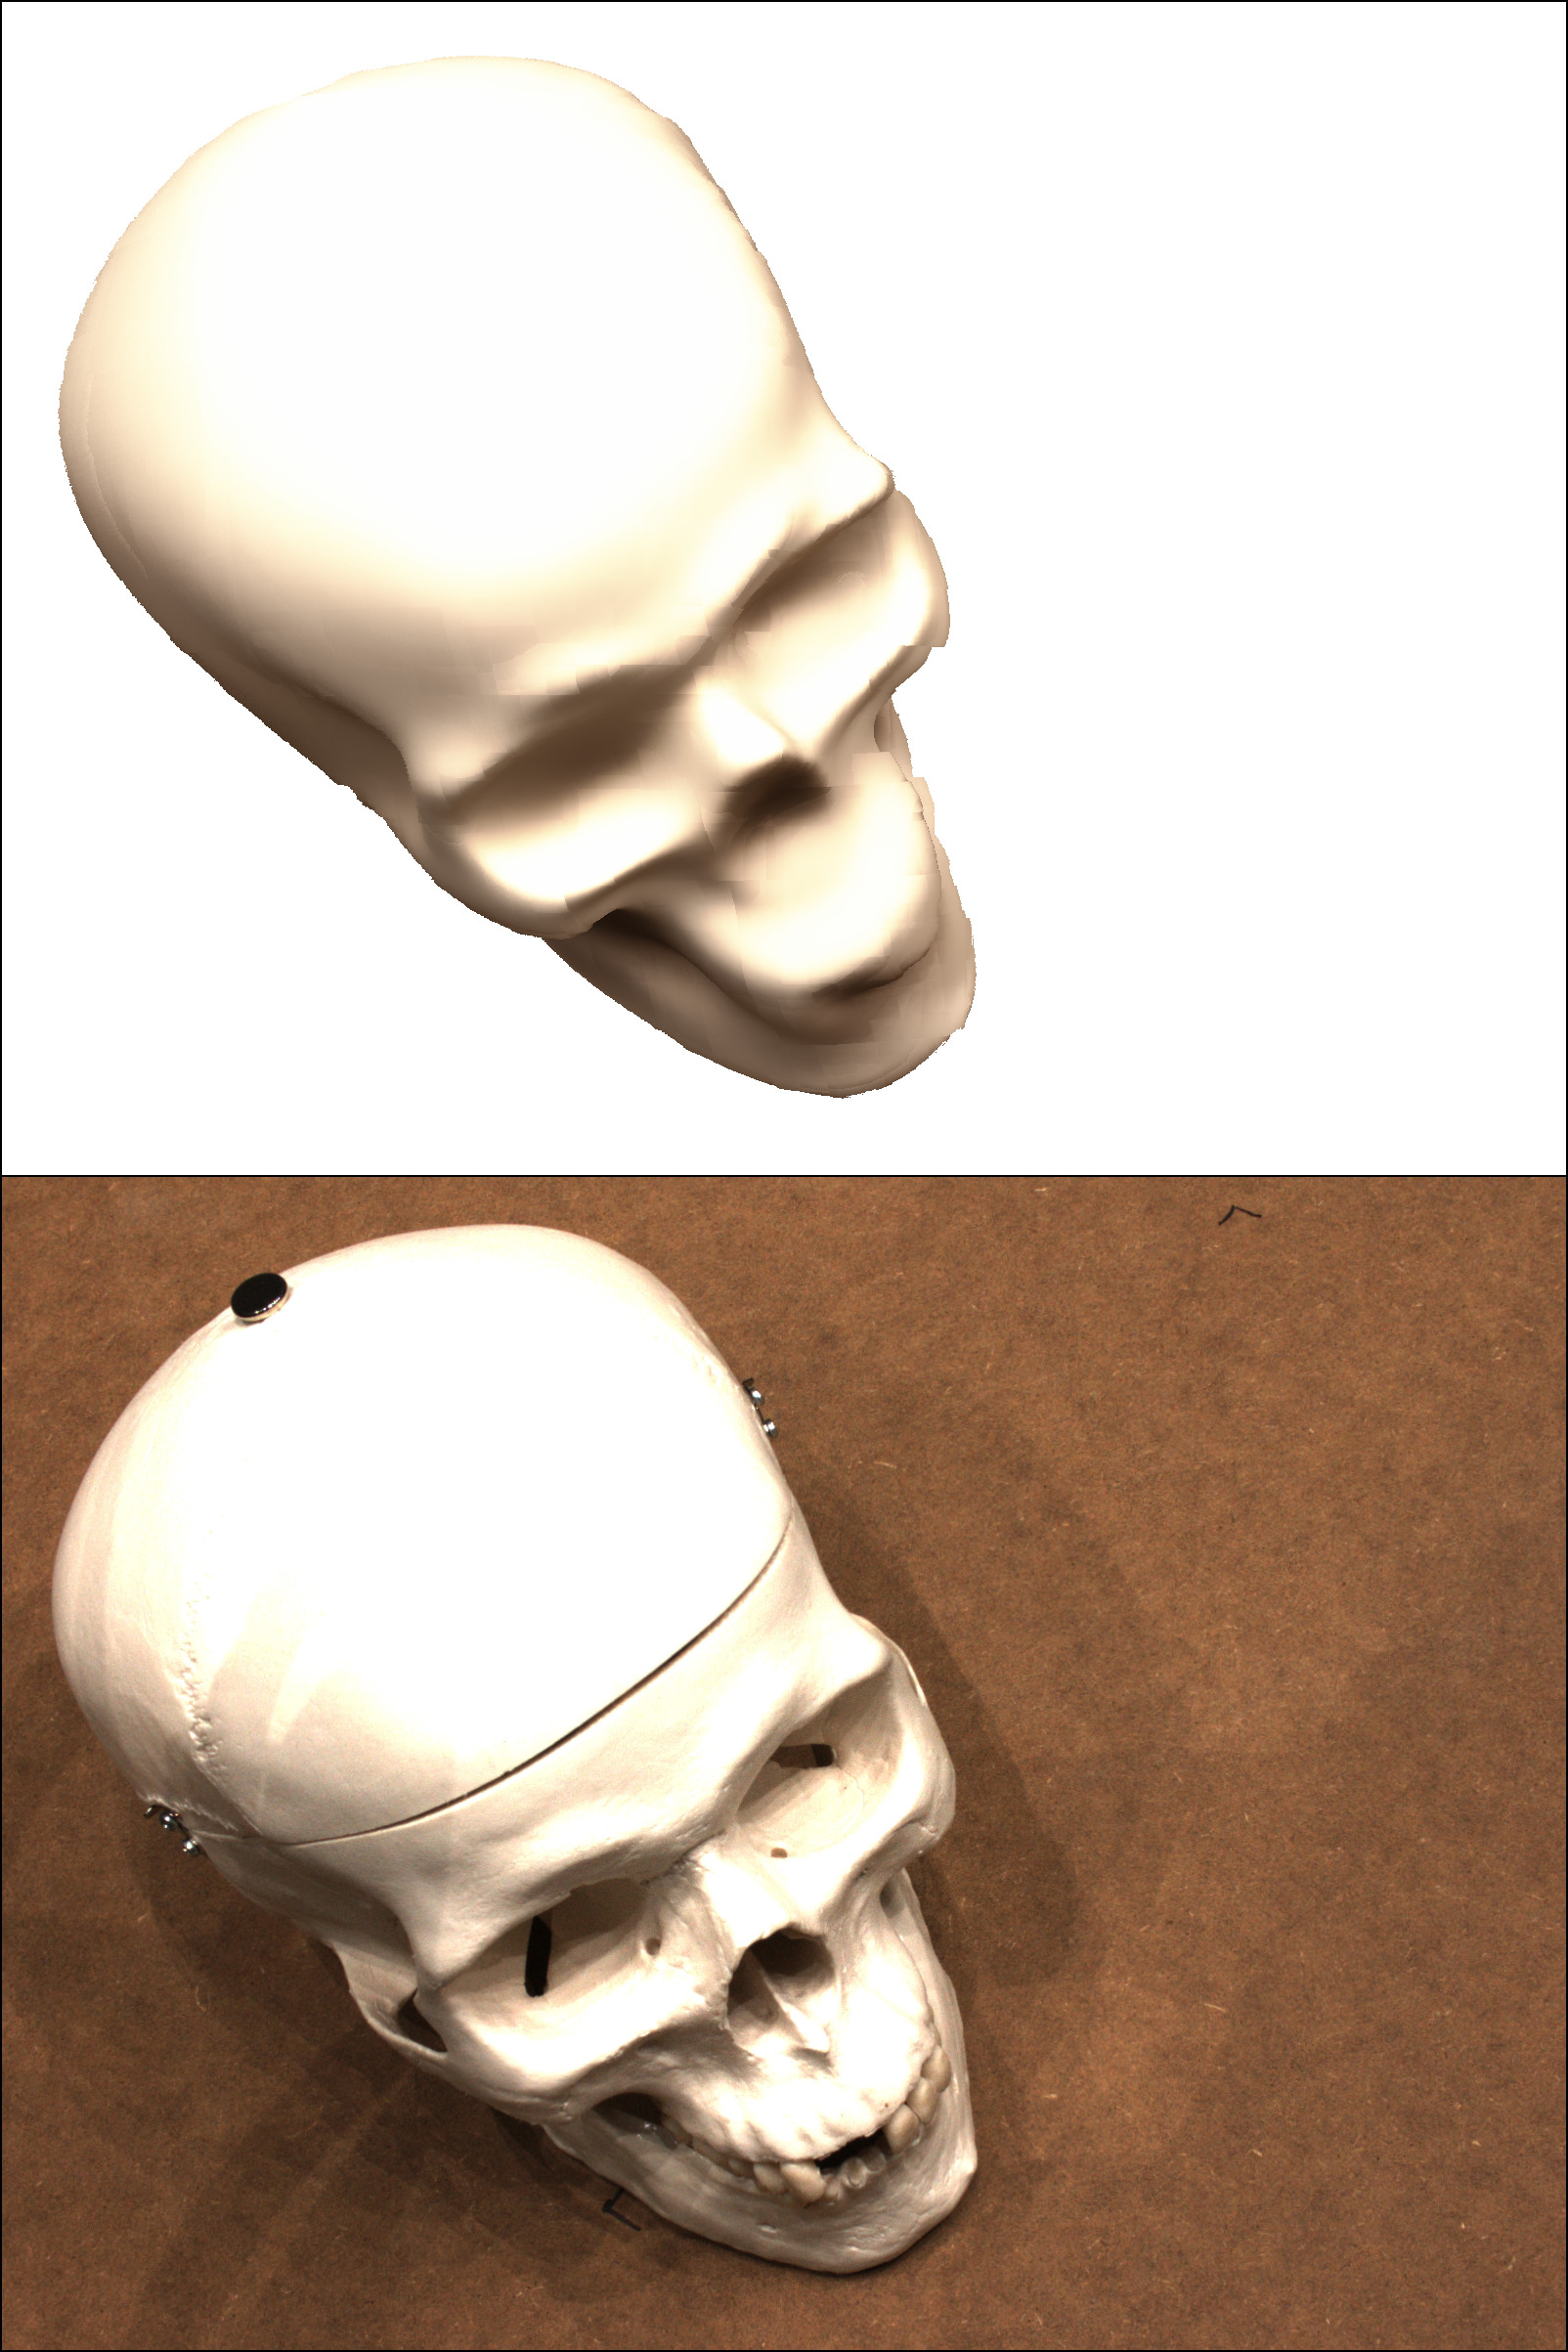
\includegraphics[width=1.5cm]{images/chapter5_img/RenderedImages-DepthMaps-EpochWise-Evals/MRHashGrid3D/65/rendering_100.jpg} & 
    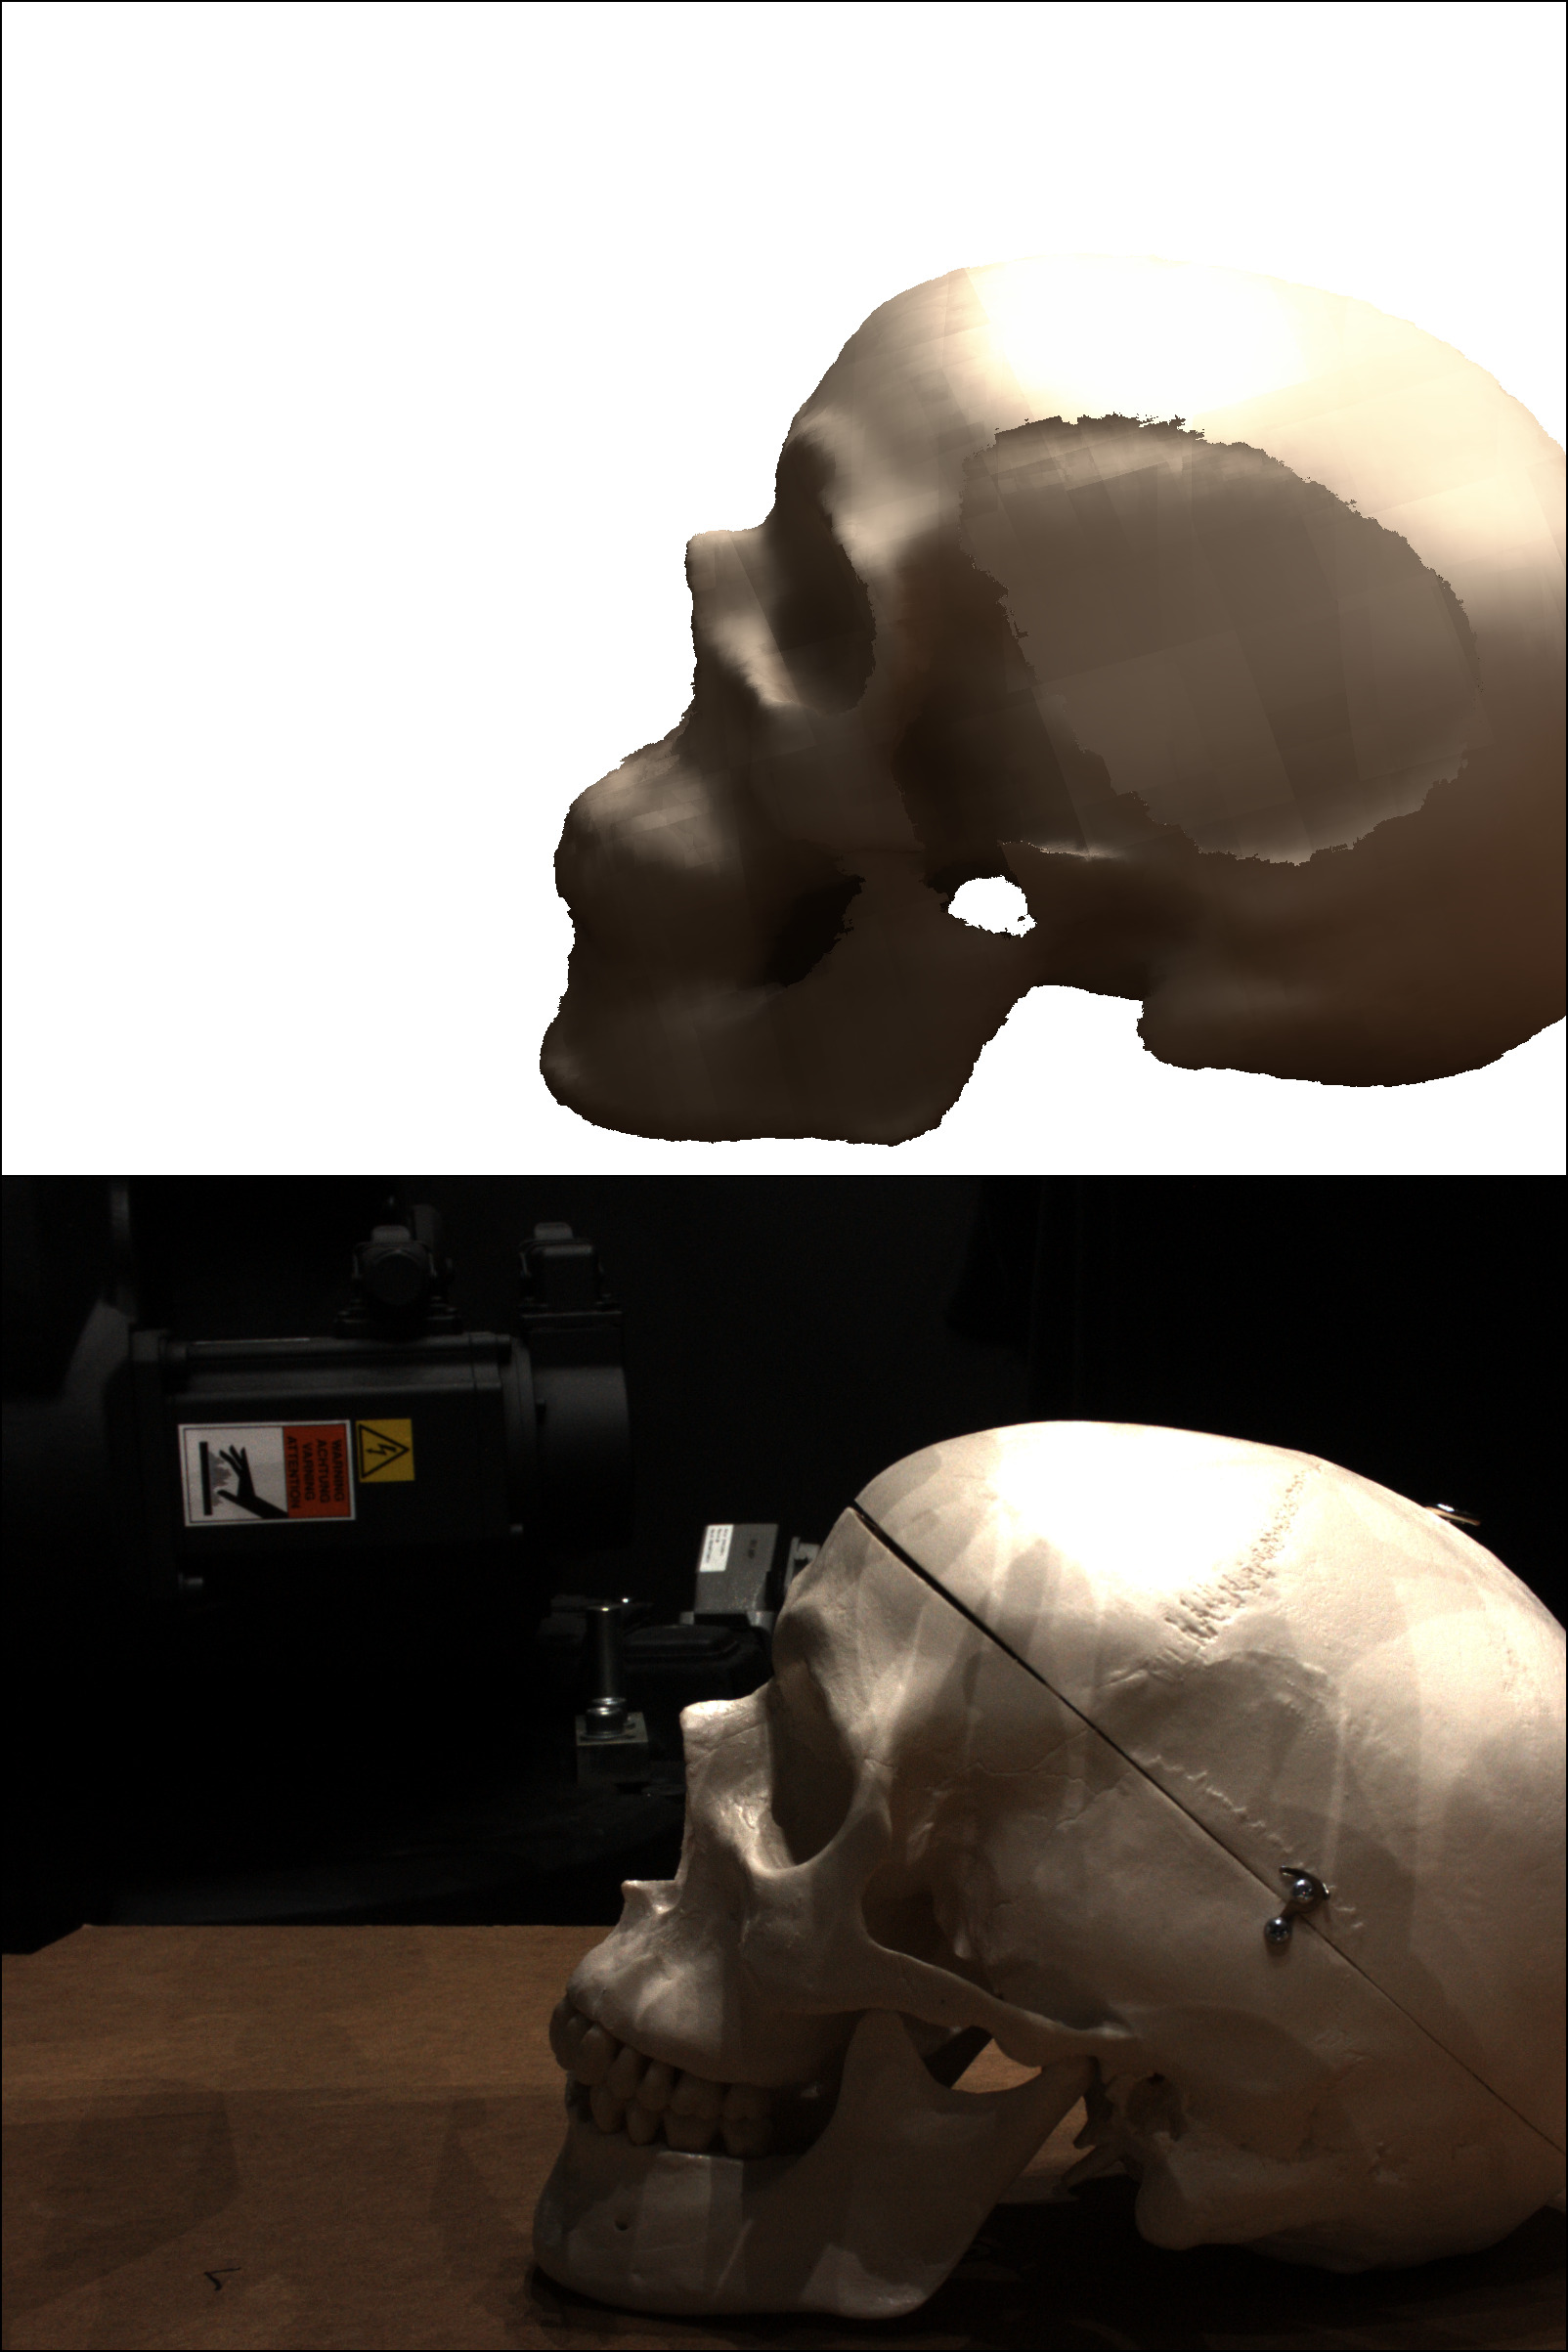
\includegraphics[width=1.5cm]{images/chapter5_img/RenderedImages-DepthMaps-EpochWise-Evals/MRHashGrid3D/65/rendering_500.jpg} & 
    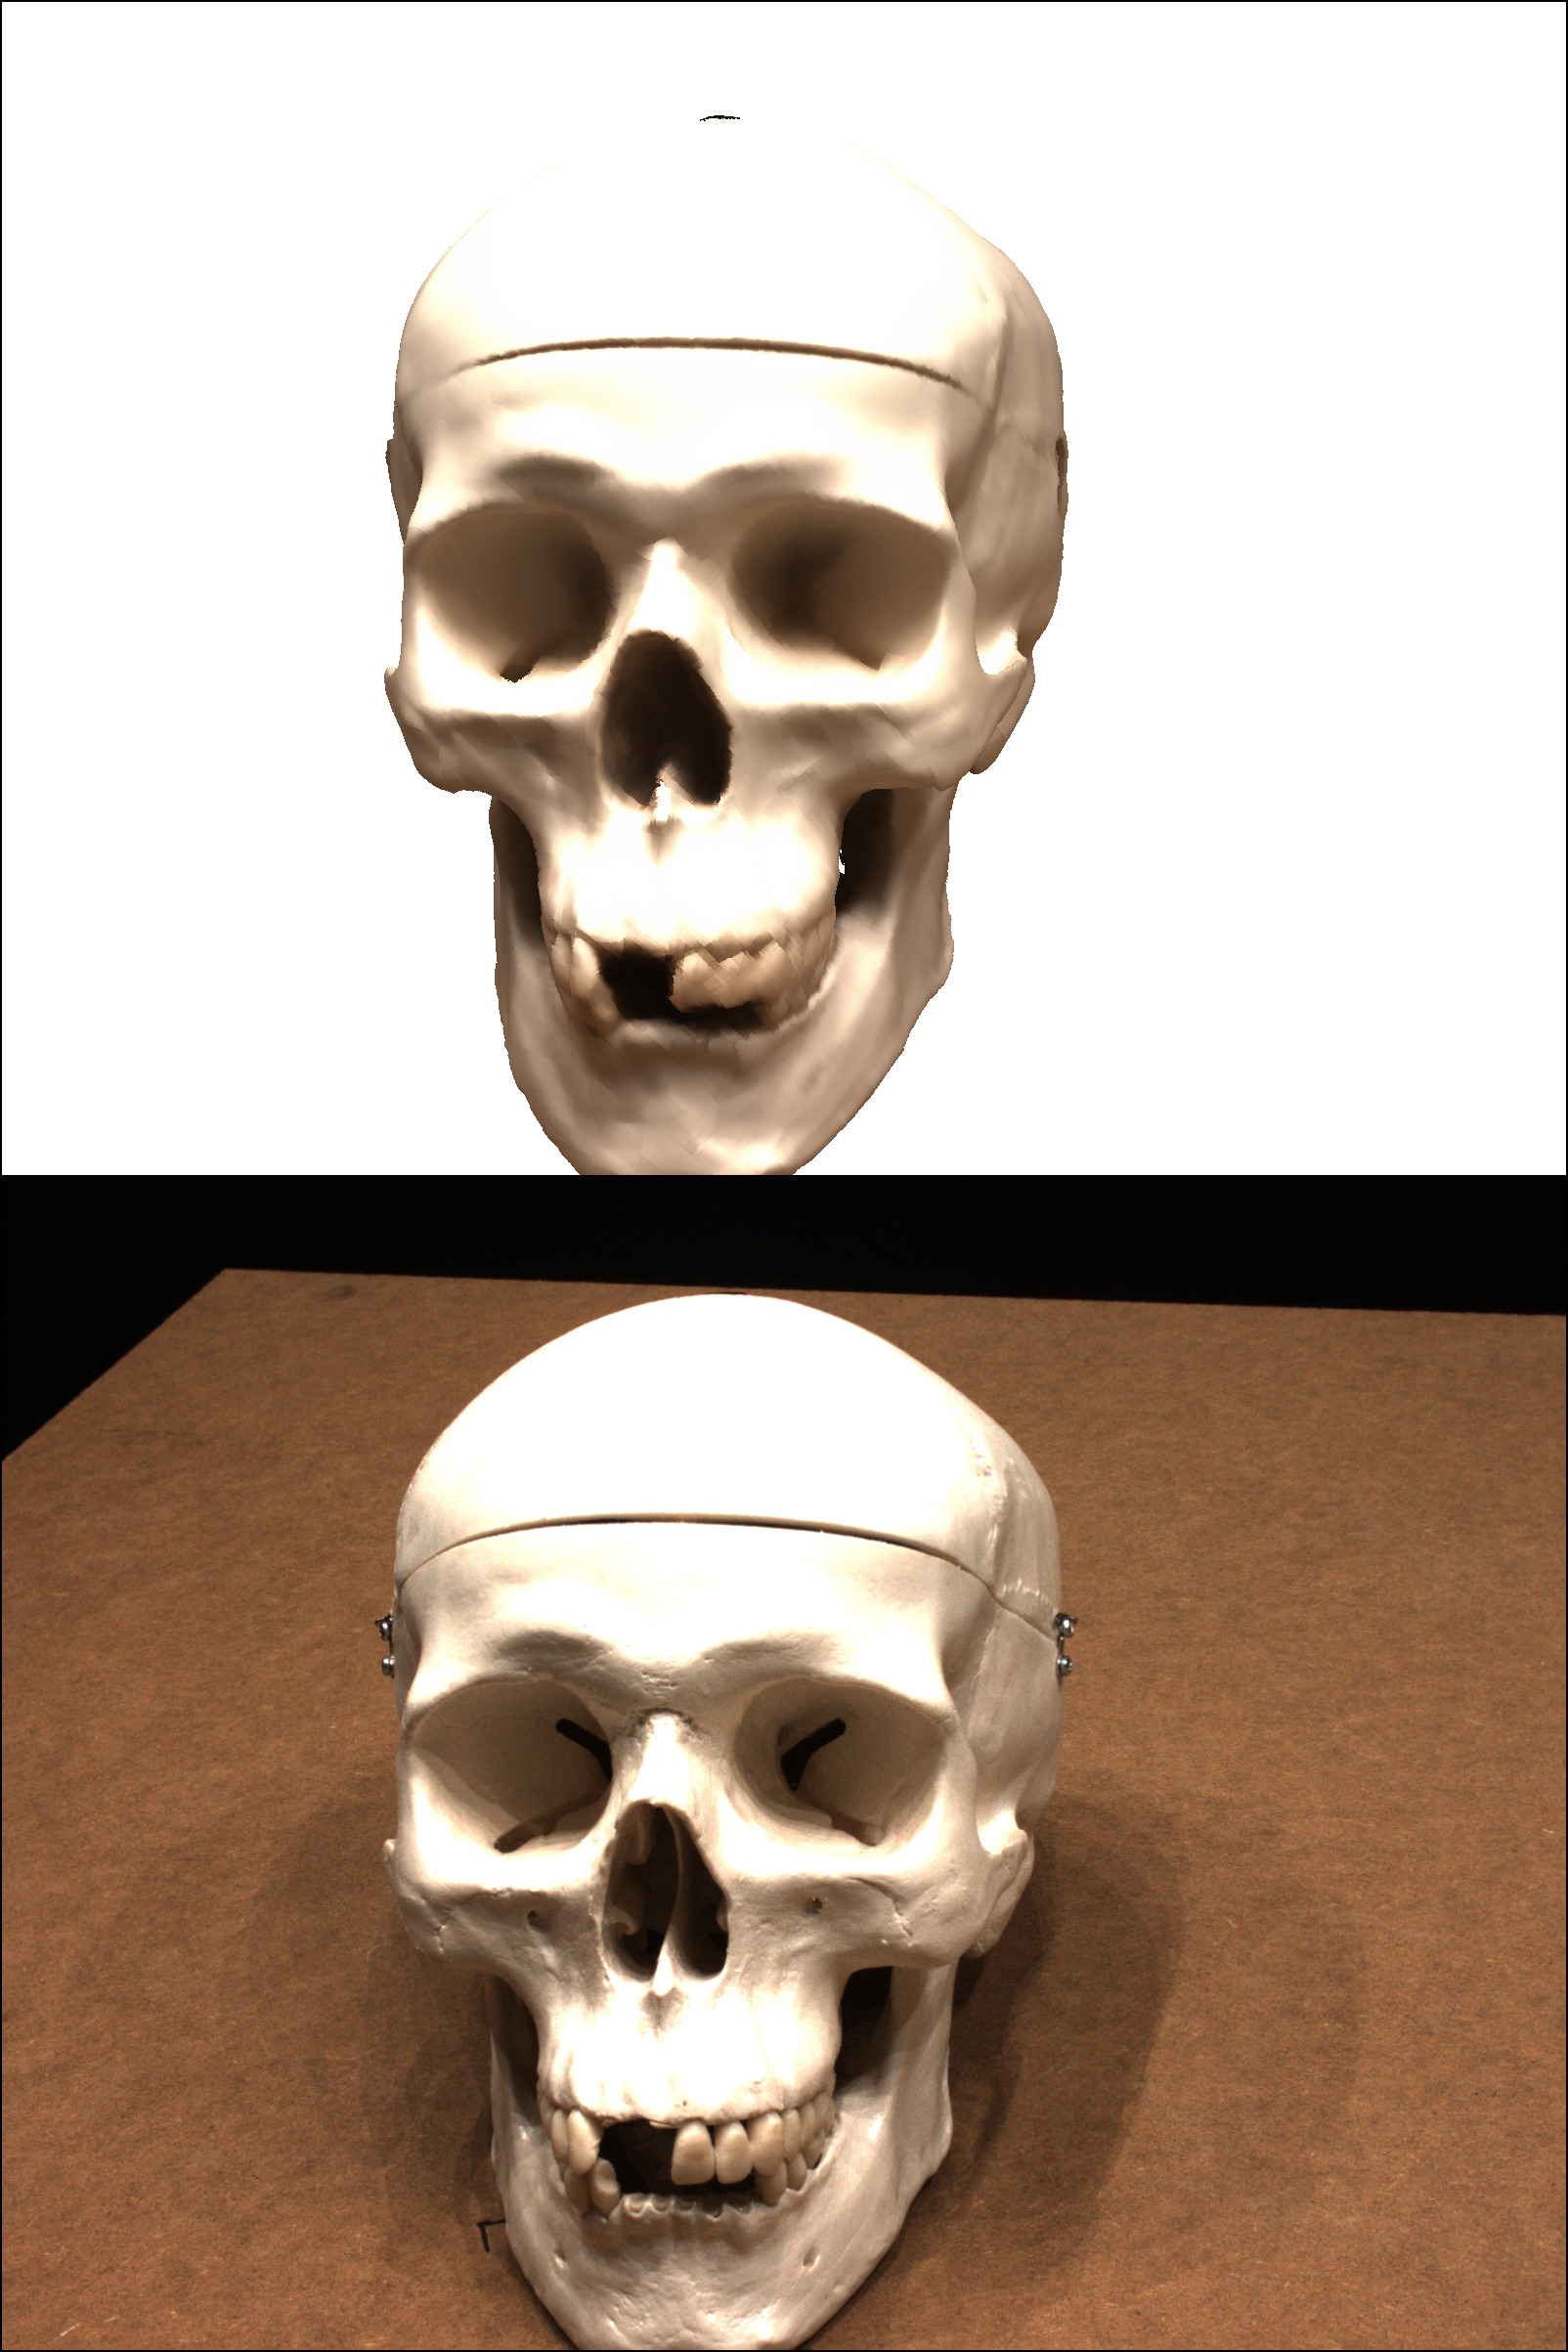
\includegraphics[width=1.5cm]{images/chapter5_img/RenderedImages-DepthMaps-EpochWise-Evals/MRHashGrid3D/65/rendering_1000.jpg} & 
    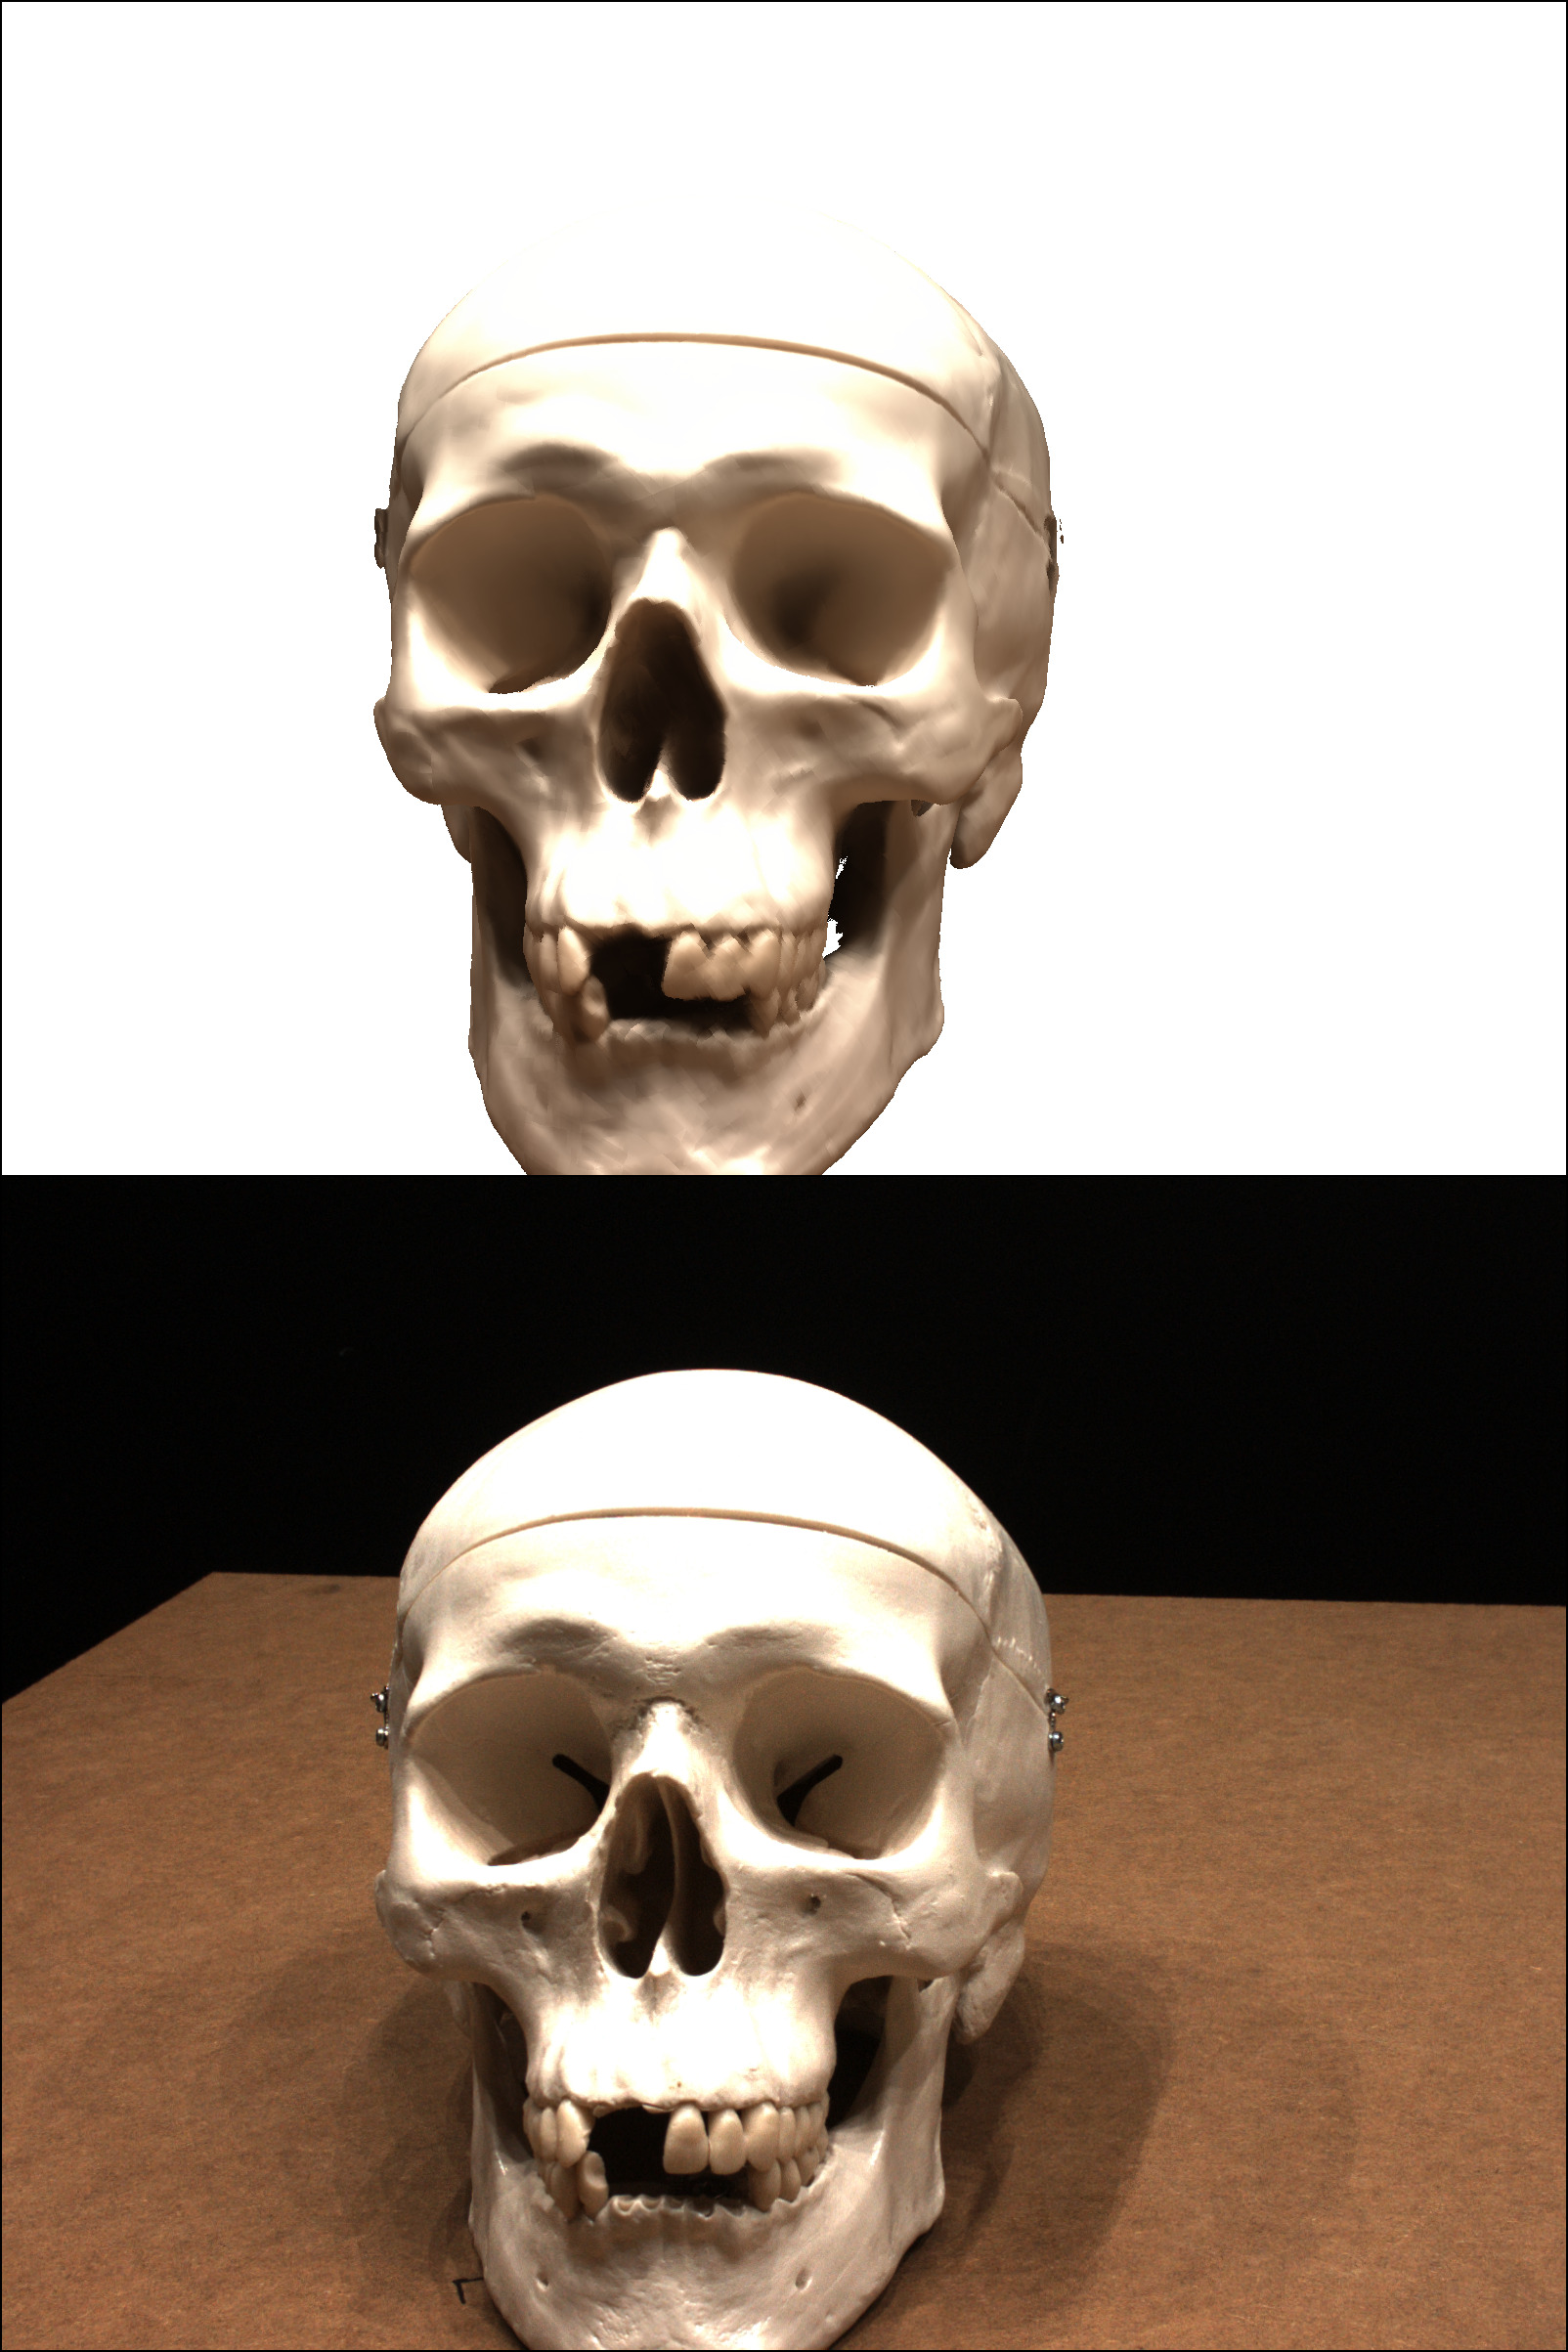
\includegraphics[width=1.5cm]{images/chapter5_img/RenderedImages-DepthMaps-EpochWise-Evals/MRHashGrid3D/65/rendering_2000.jpg} & 
    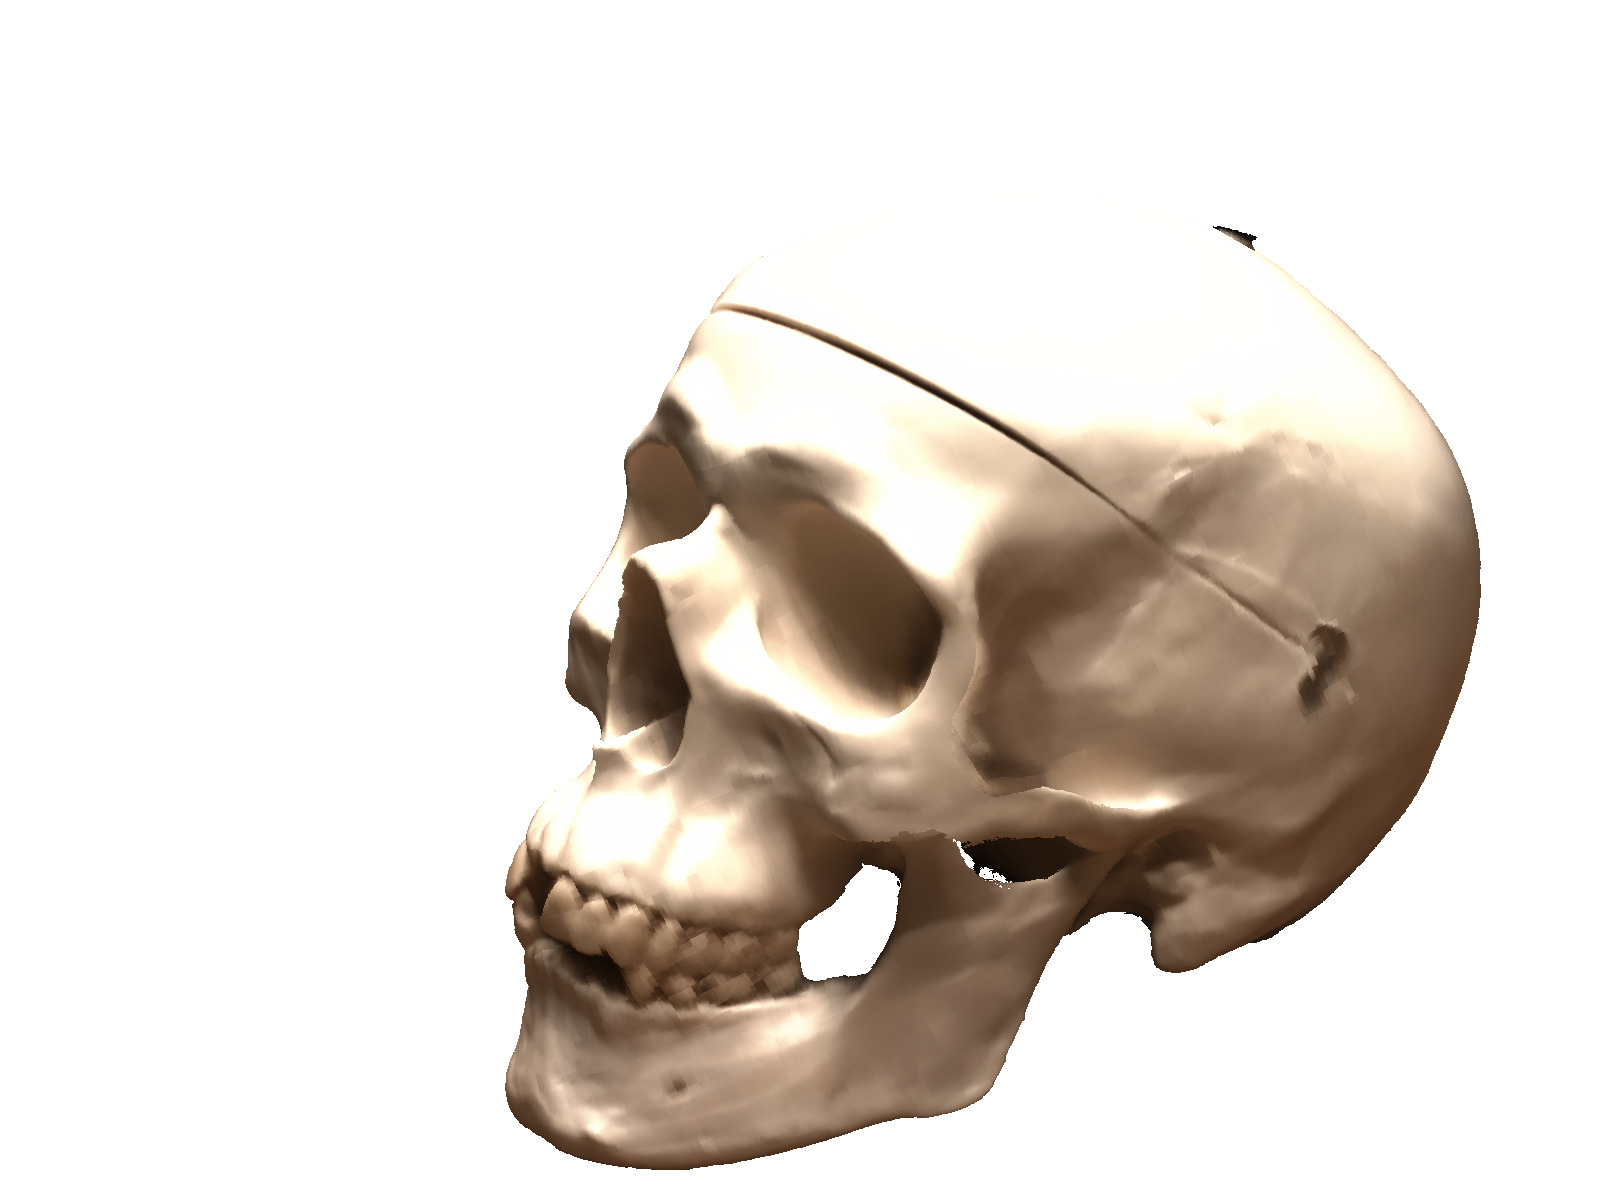
\includegraphics[width=1.5cm]{images/chapter5_img/RenderedImages-DepthMaps-EpochWise-Evals/MRHashGrid3D/65/eval_035.jpg} \\
    \hline 
    NFFB & 
    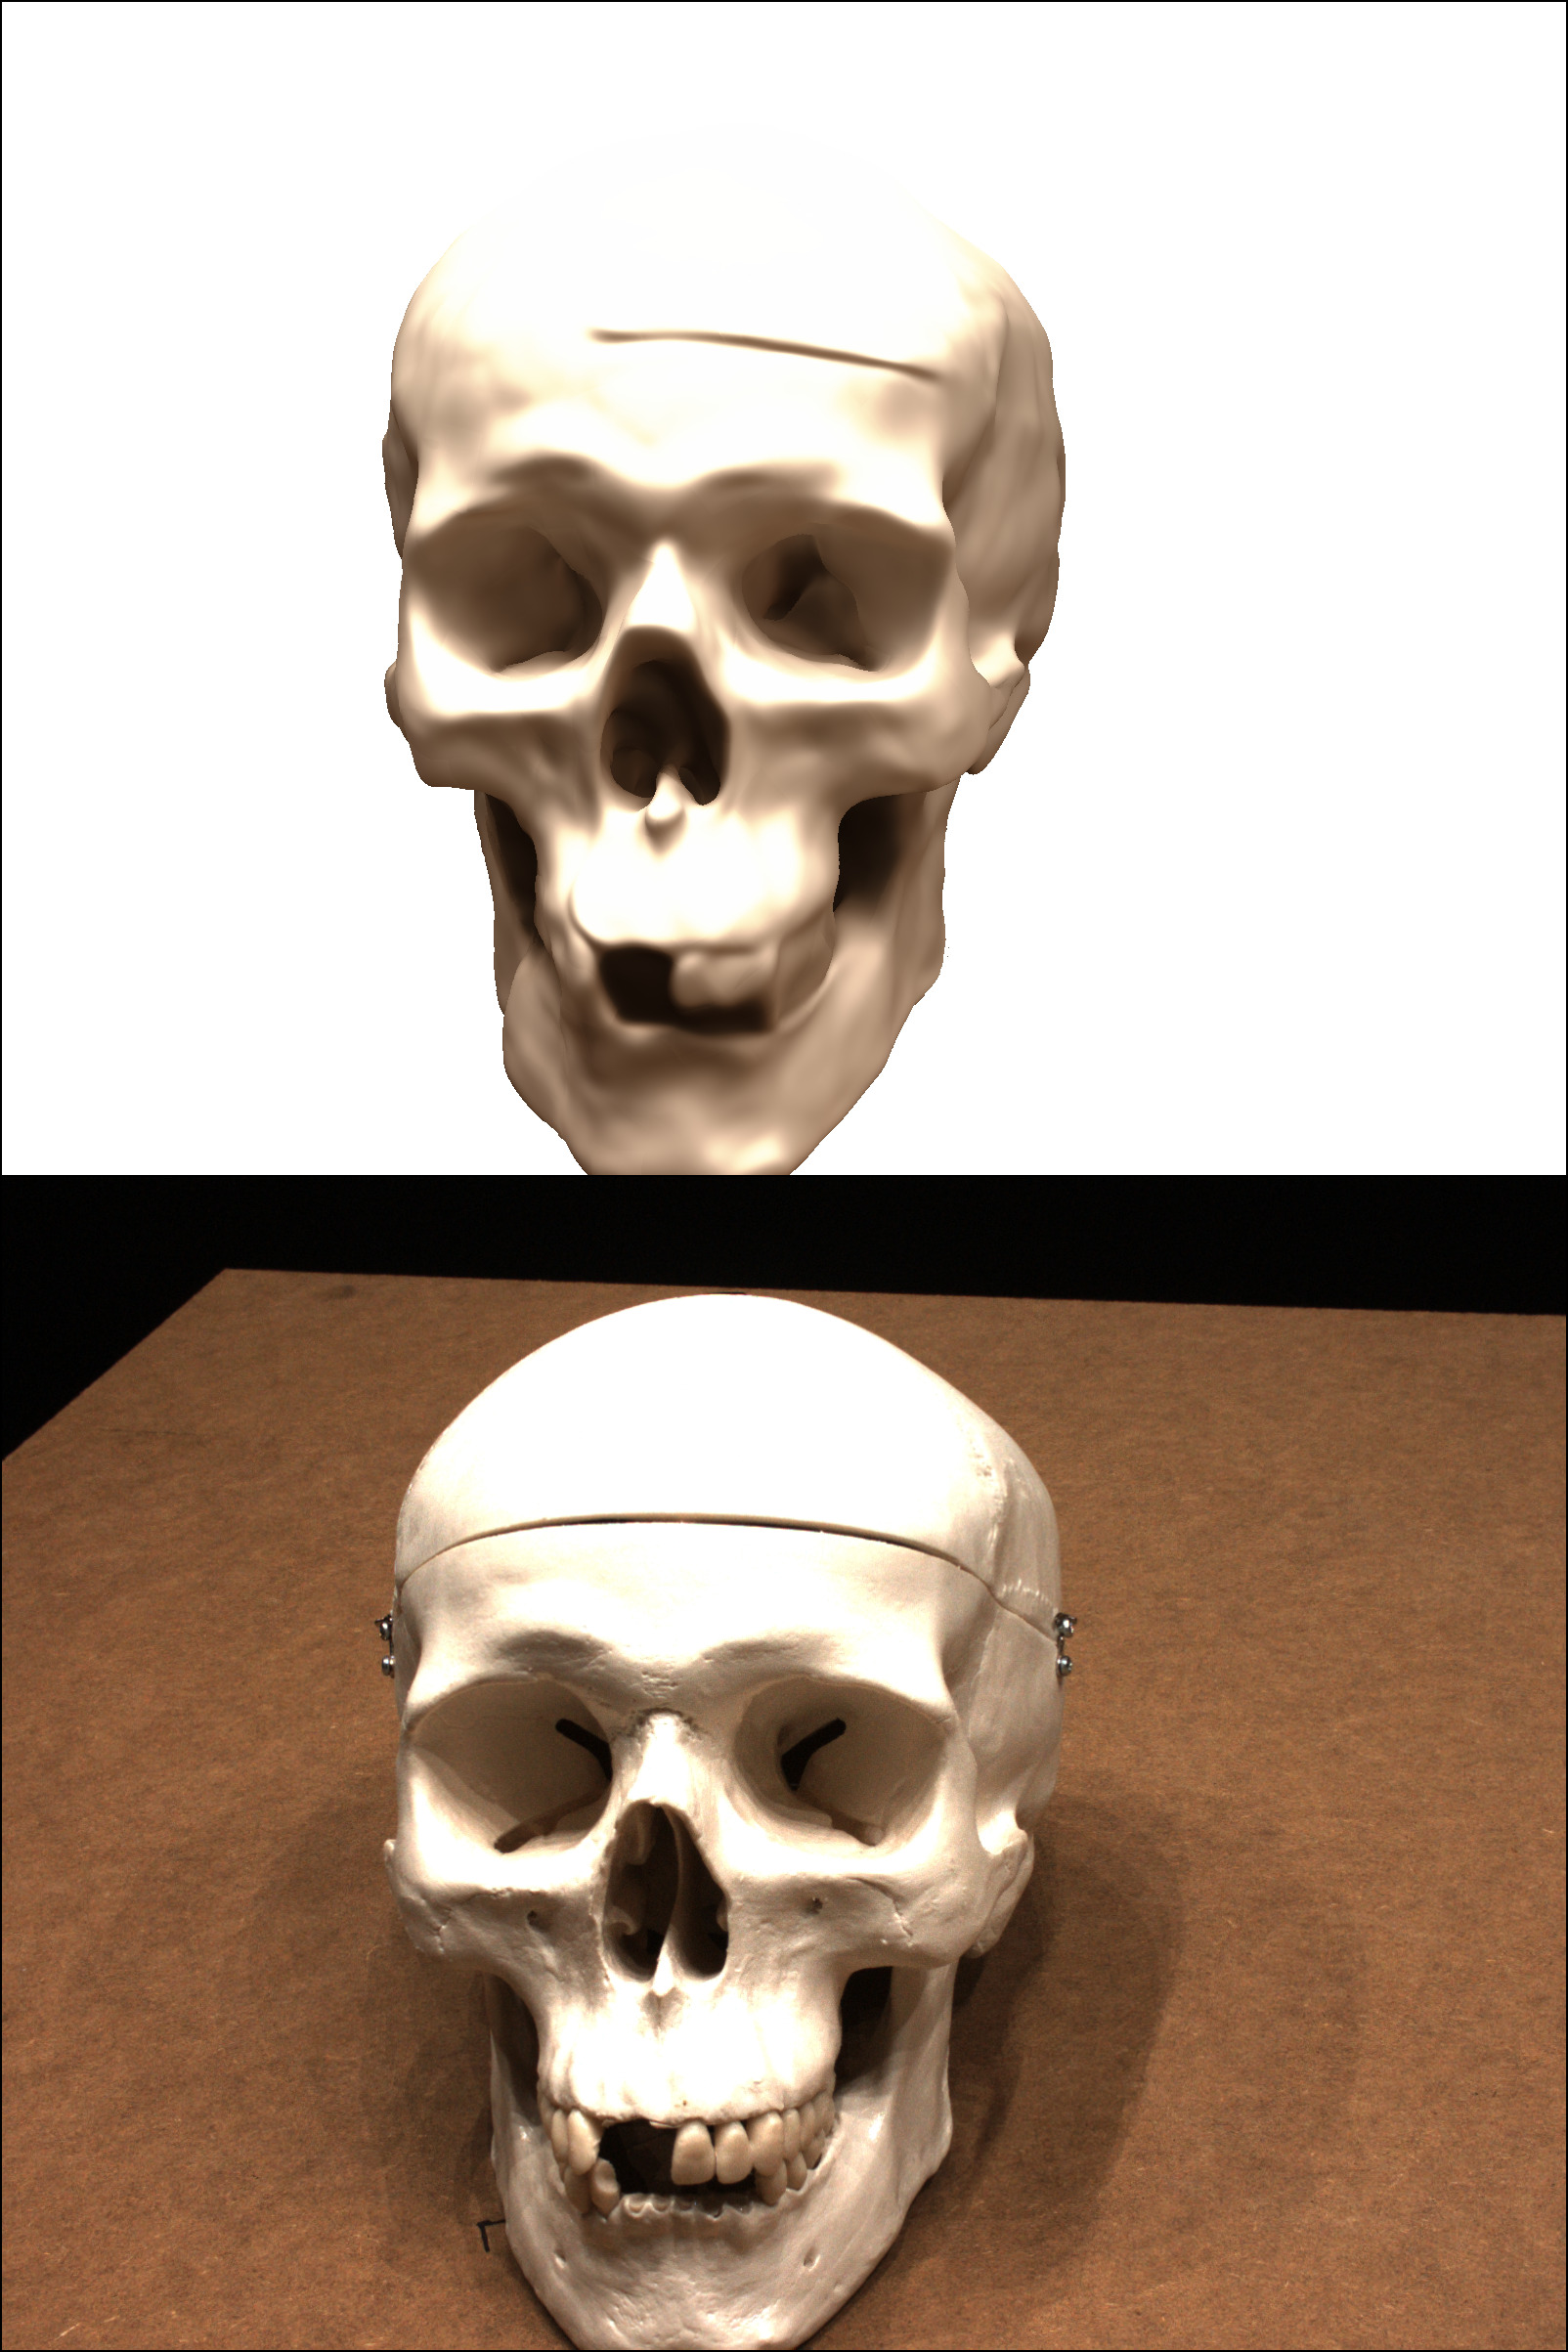
\includegraphics[width=1.5cm]{images/chapter5_img/RenderedImages-DepthMaps-EpochWise-Evals/NFFB/65/rendering_100.jpg} & 
    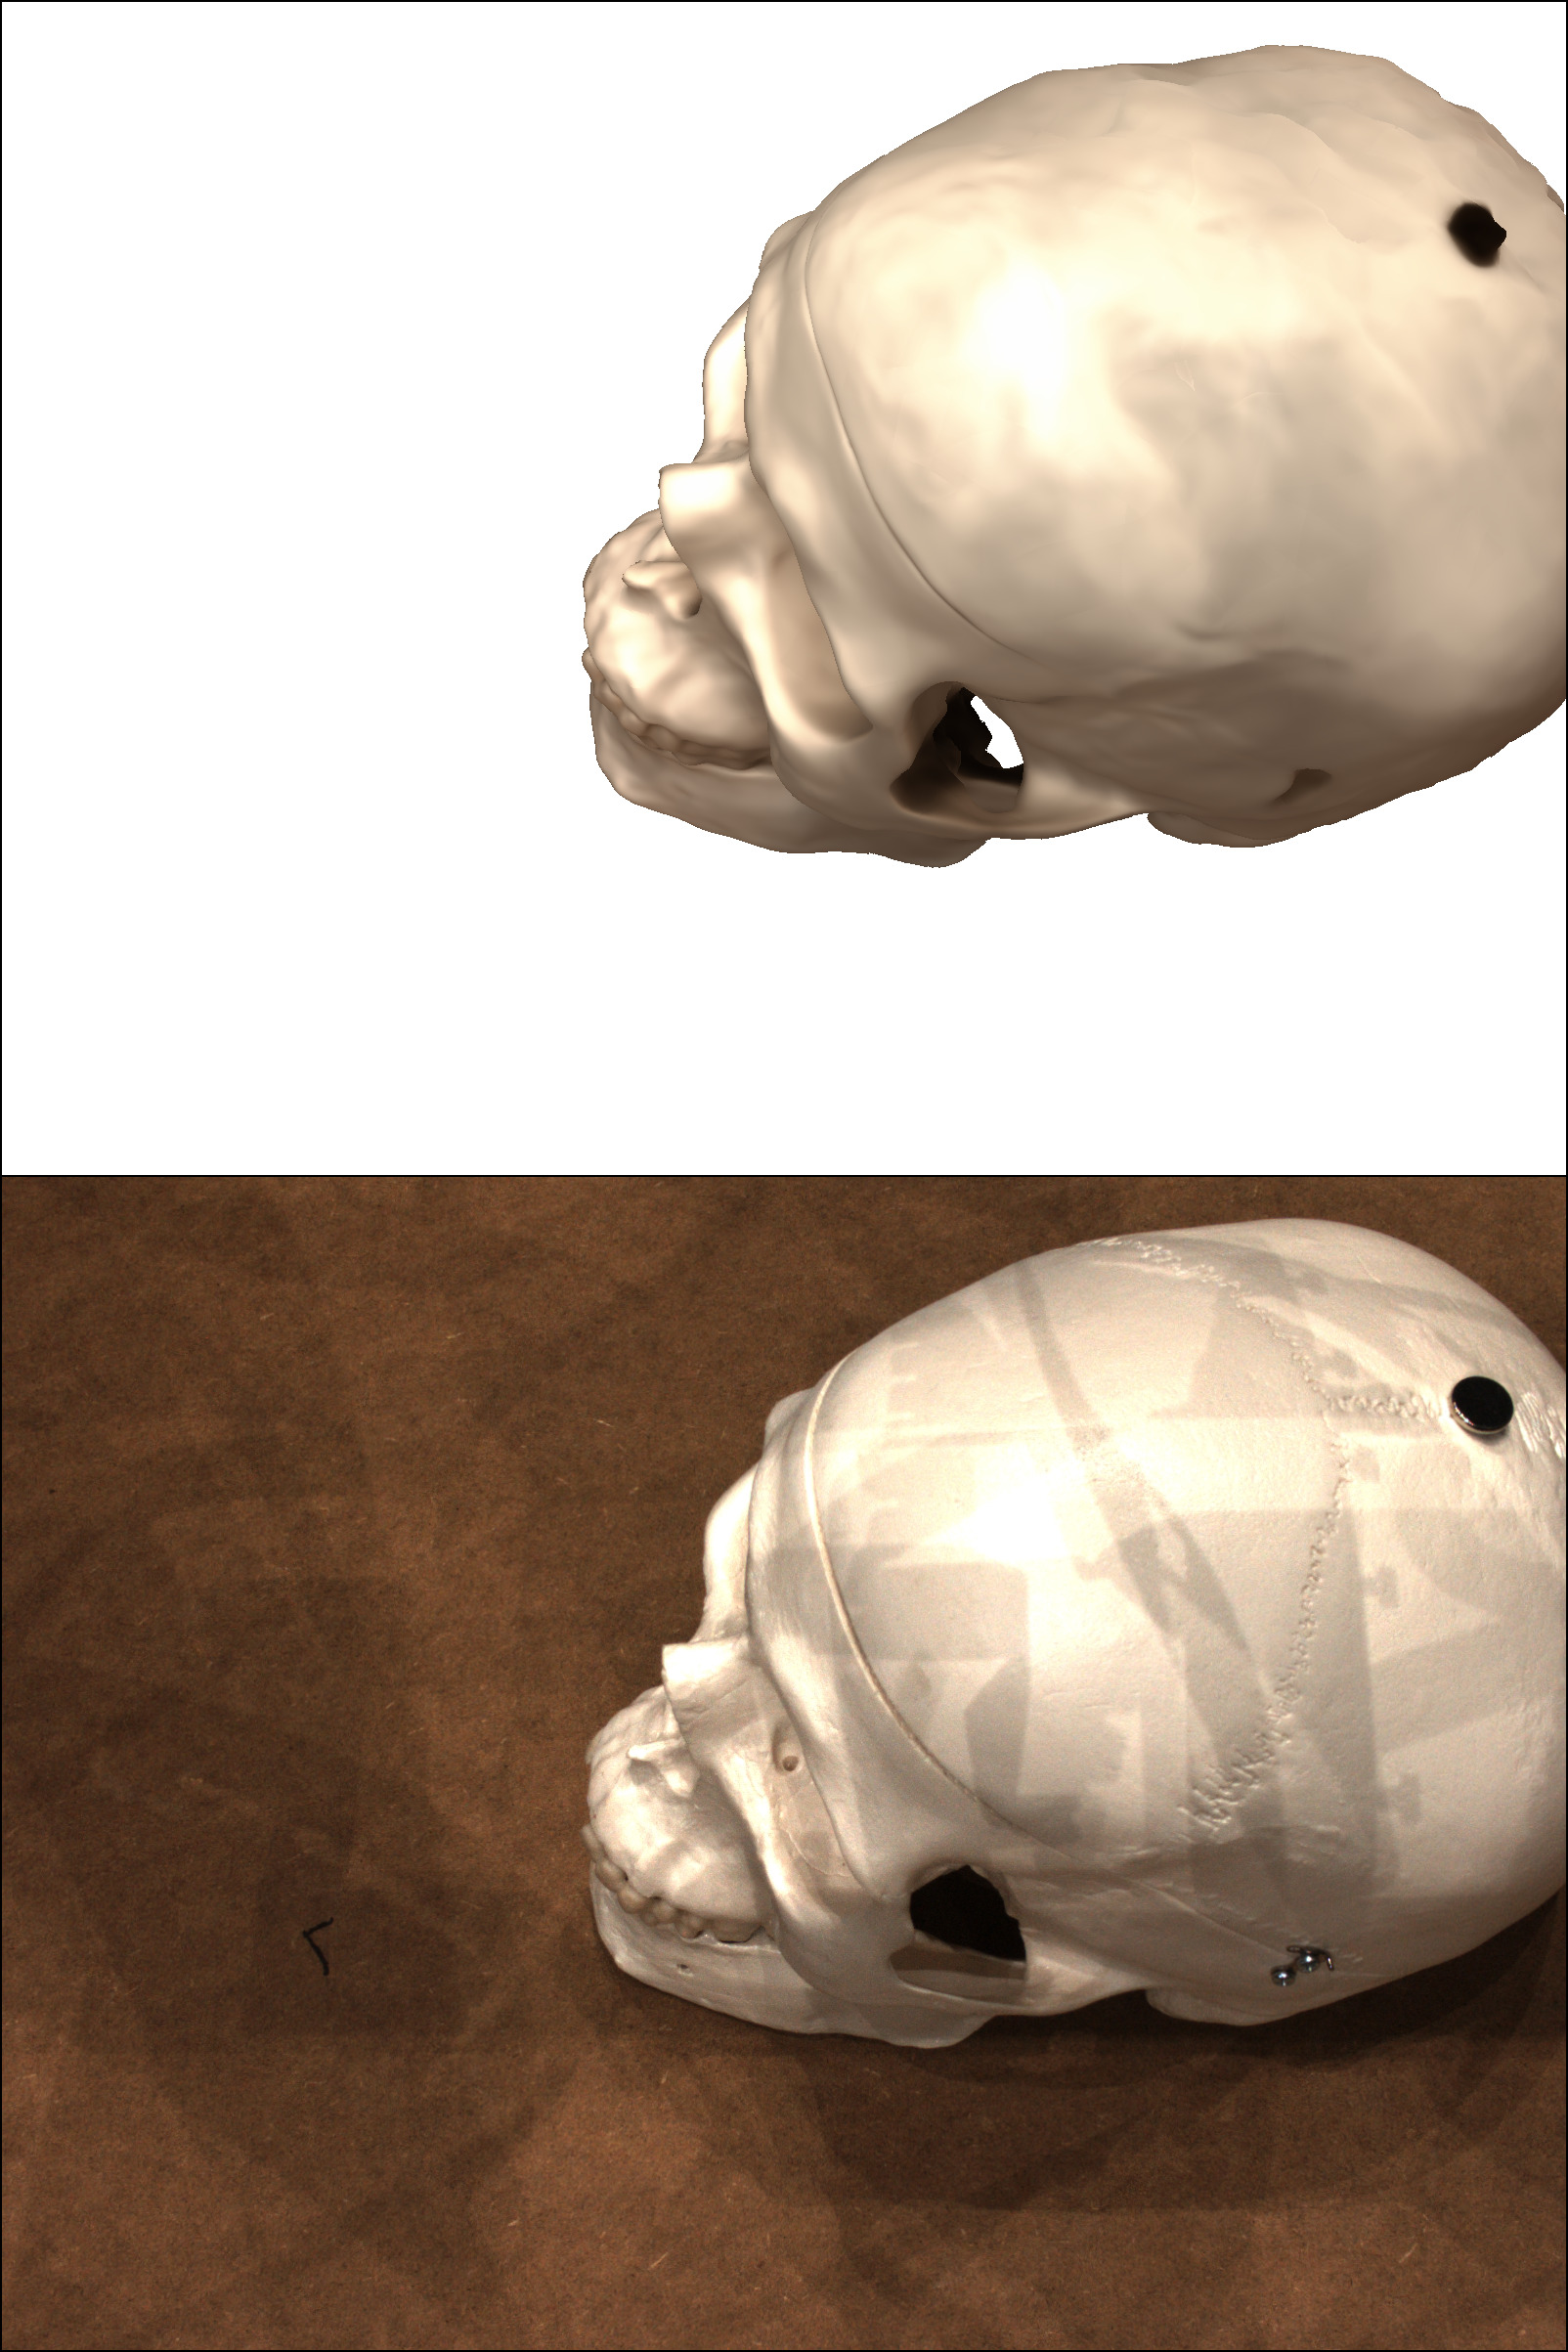
\includegraphics[width=1.5cm]{images/chapter5_img/RenderedImages-DepthMaps-EpochWise-Evals/NFFB/65/rendering_500.jpg} & 
    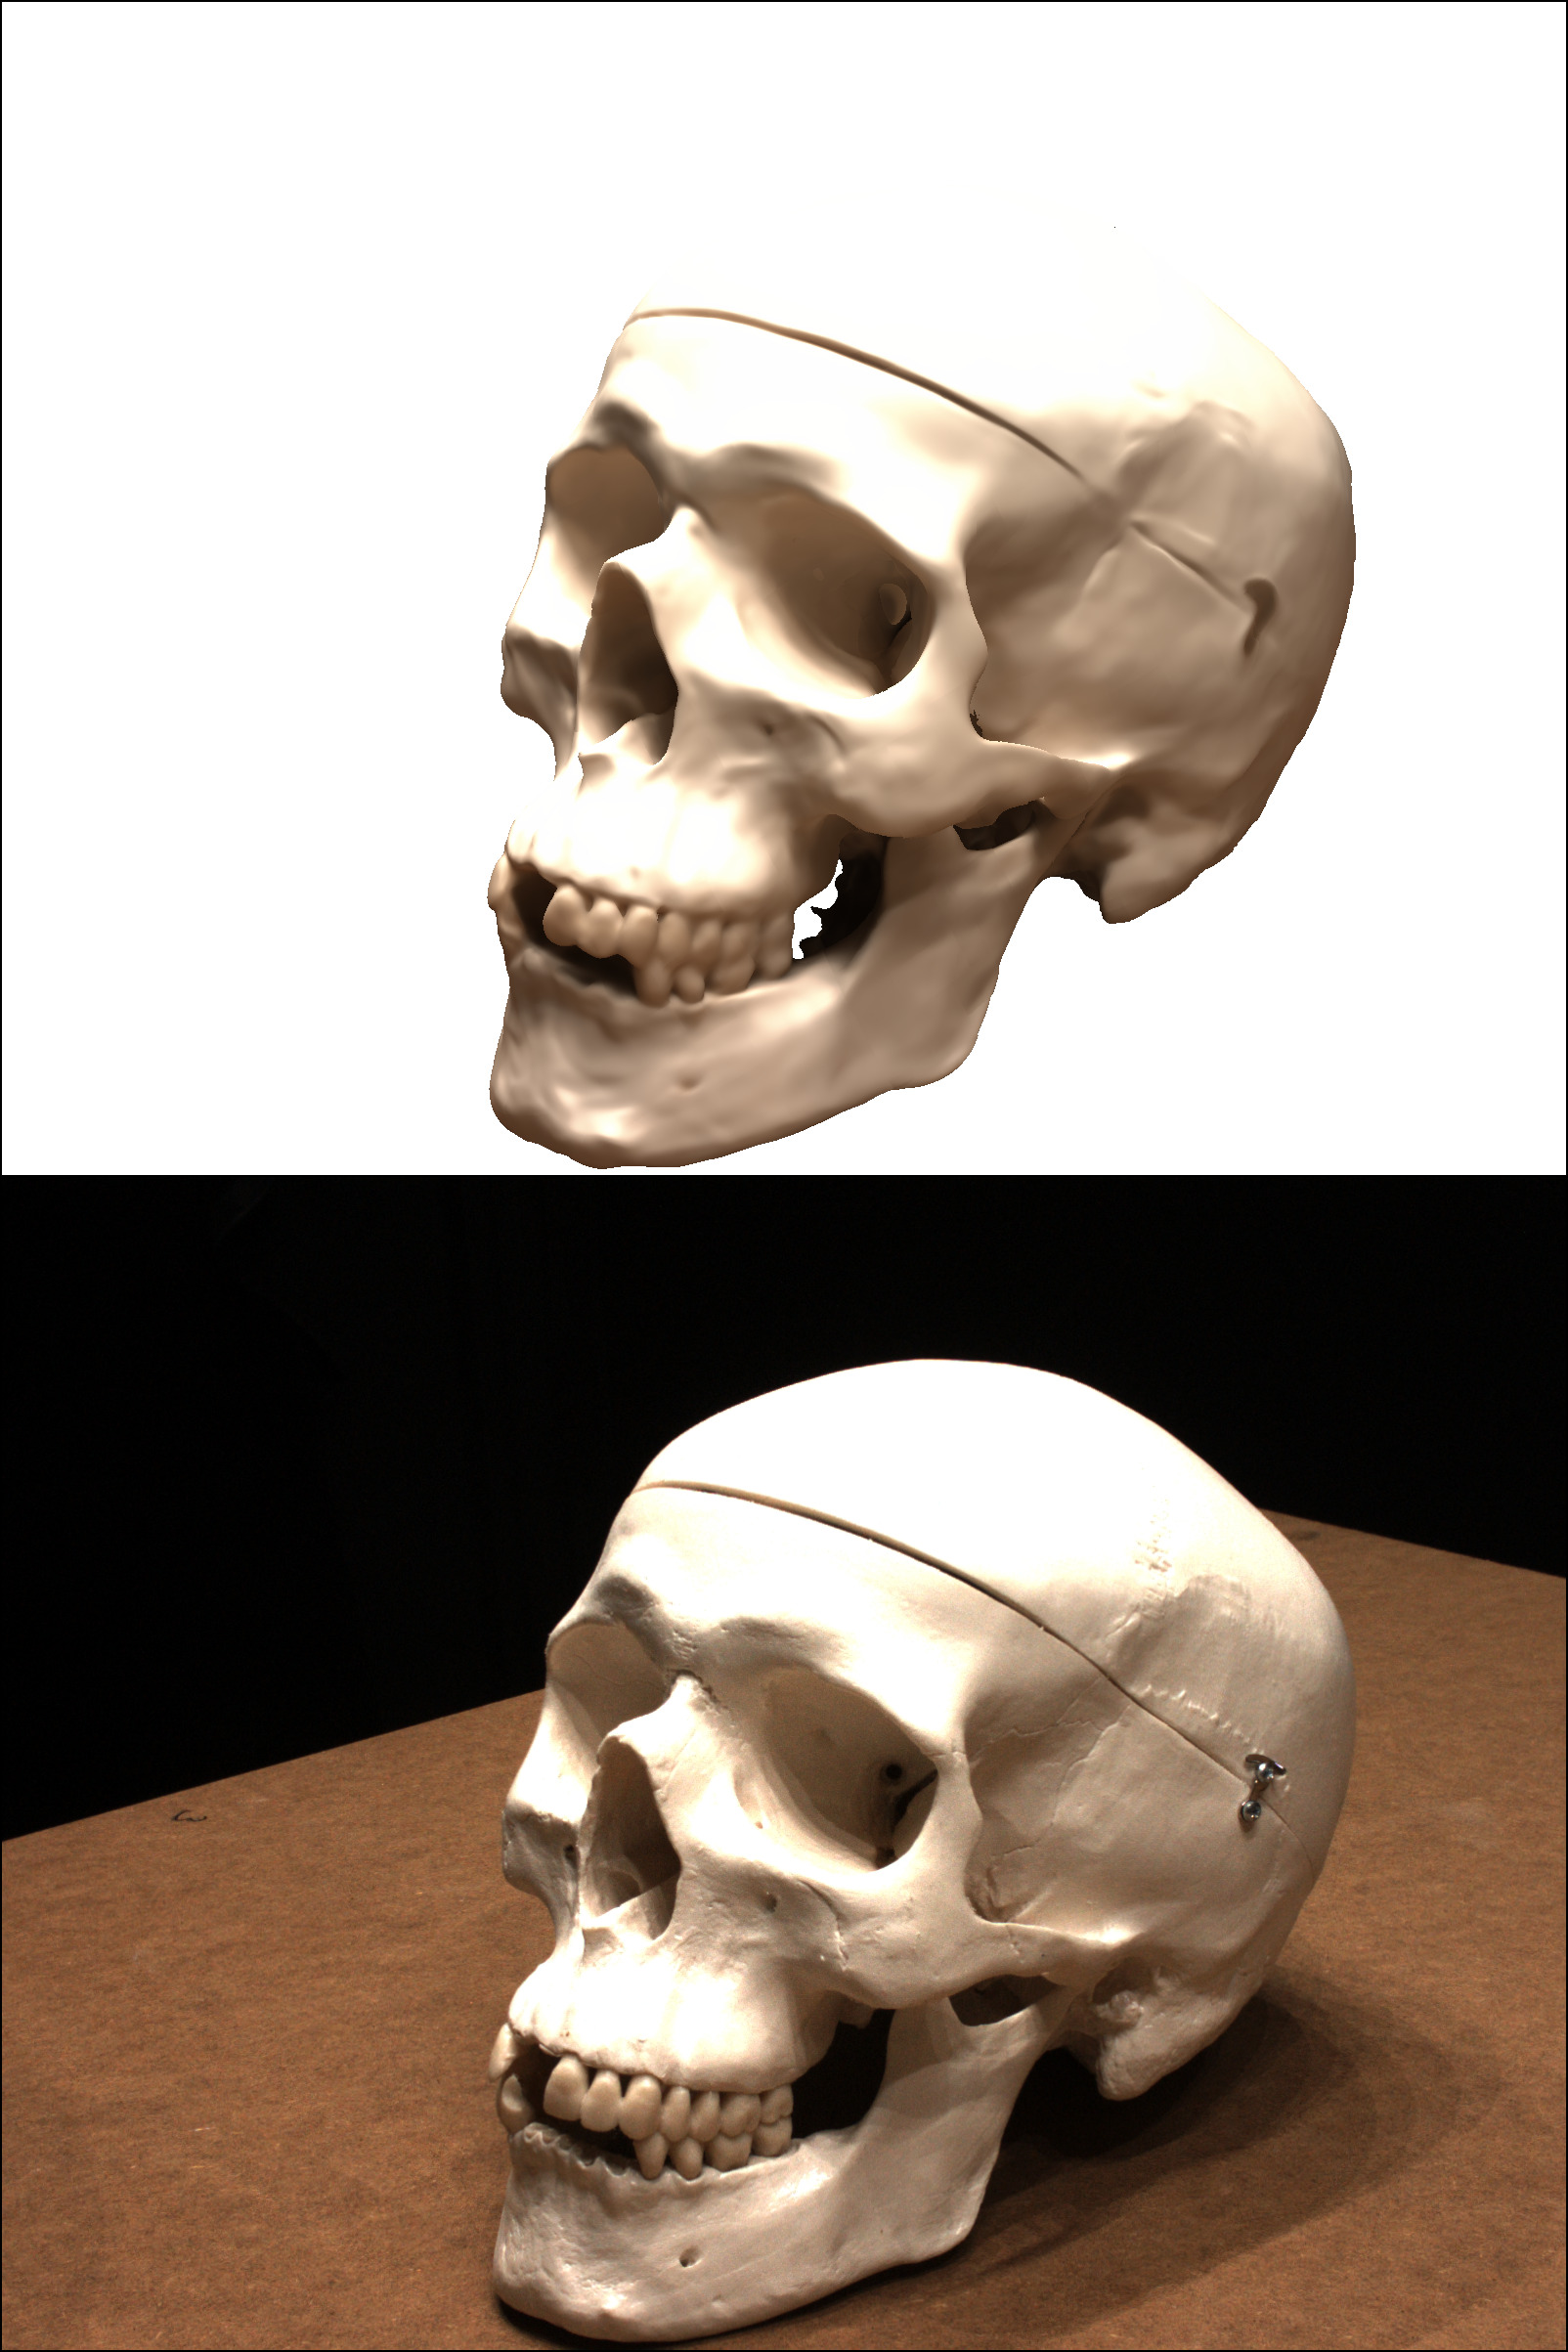
\includegraphics[width=1.5cm]{images/chapter5_img/RenderedImages-DepthMaps-EpochWise-Evals/NFFB/65/rendering_1000.jpg} & 
    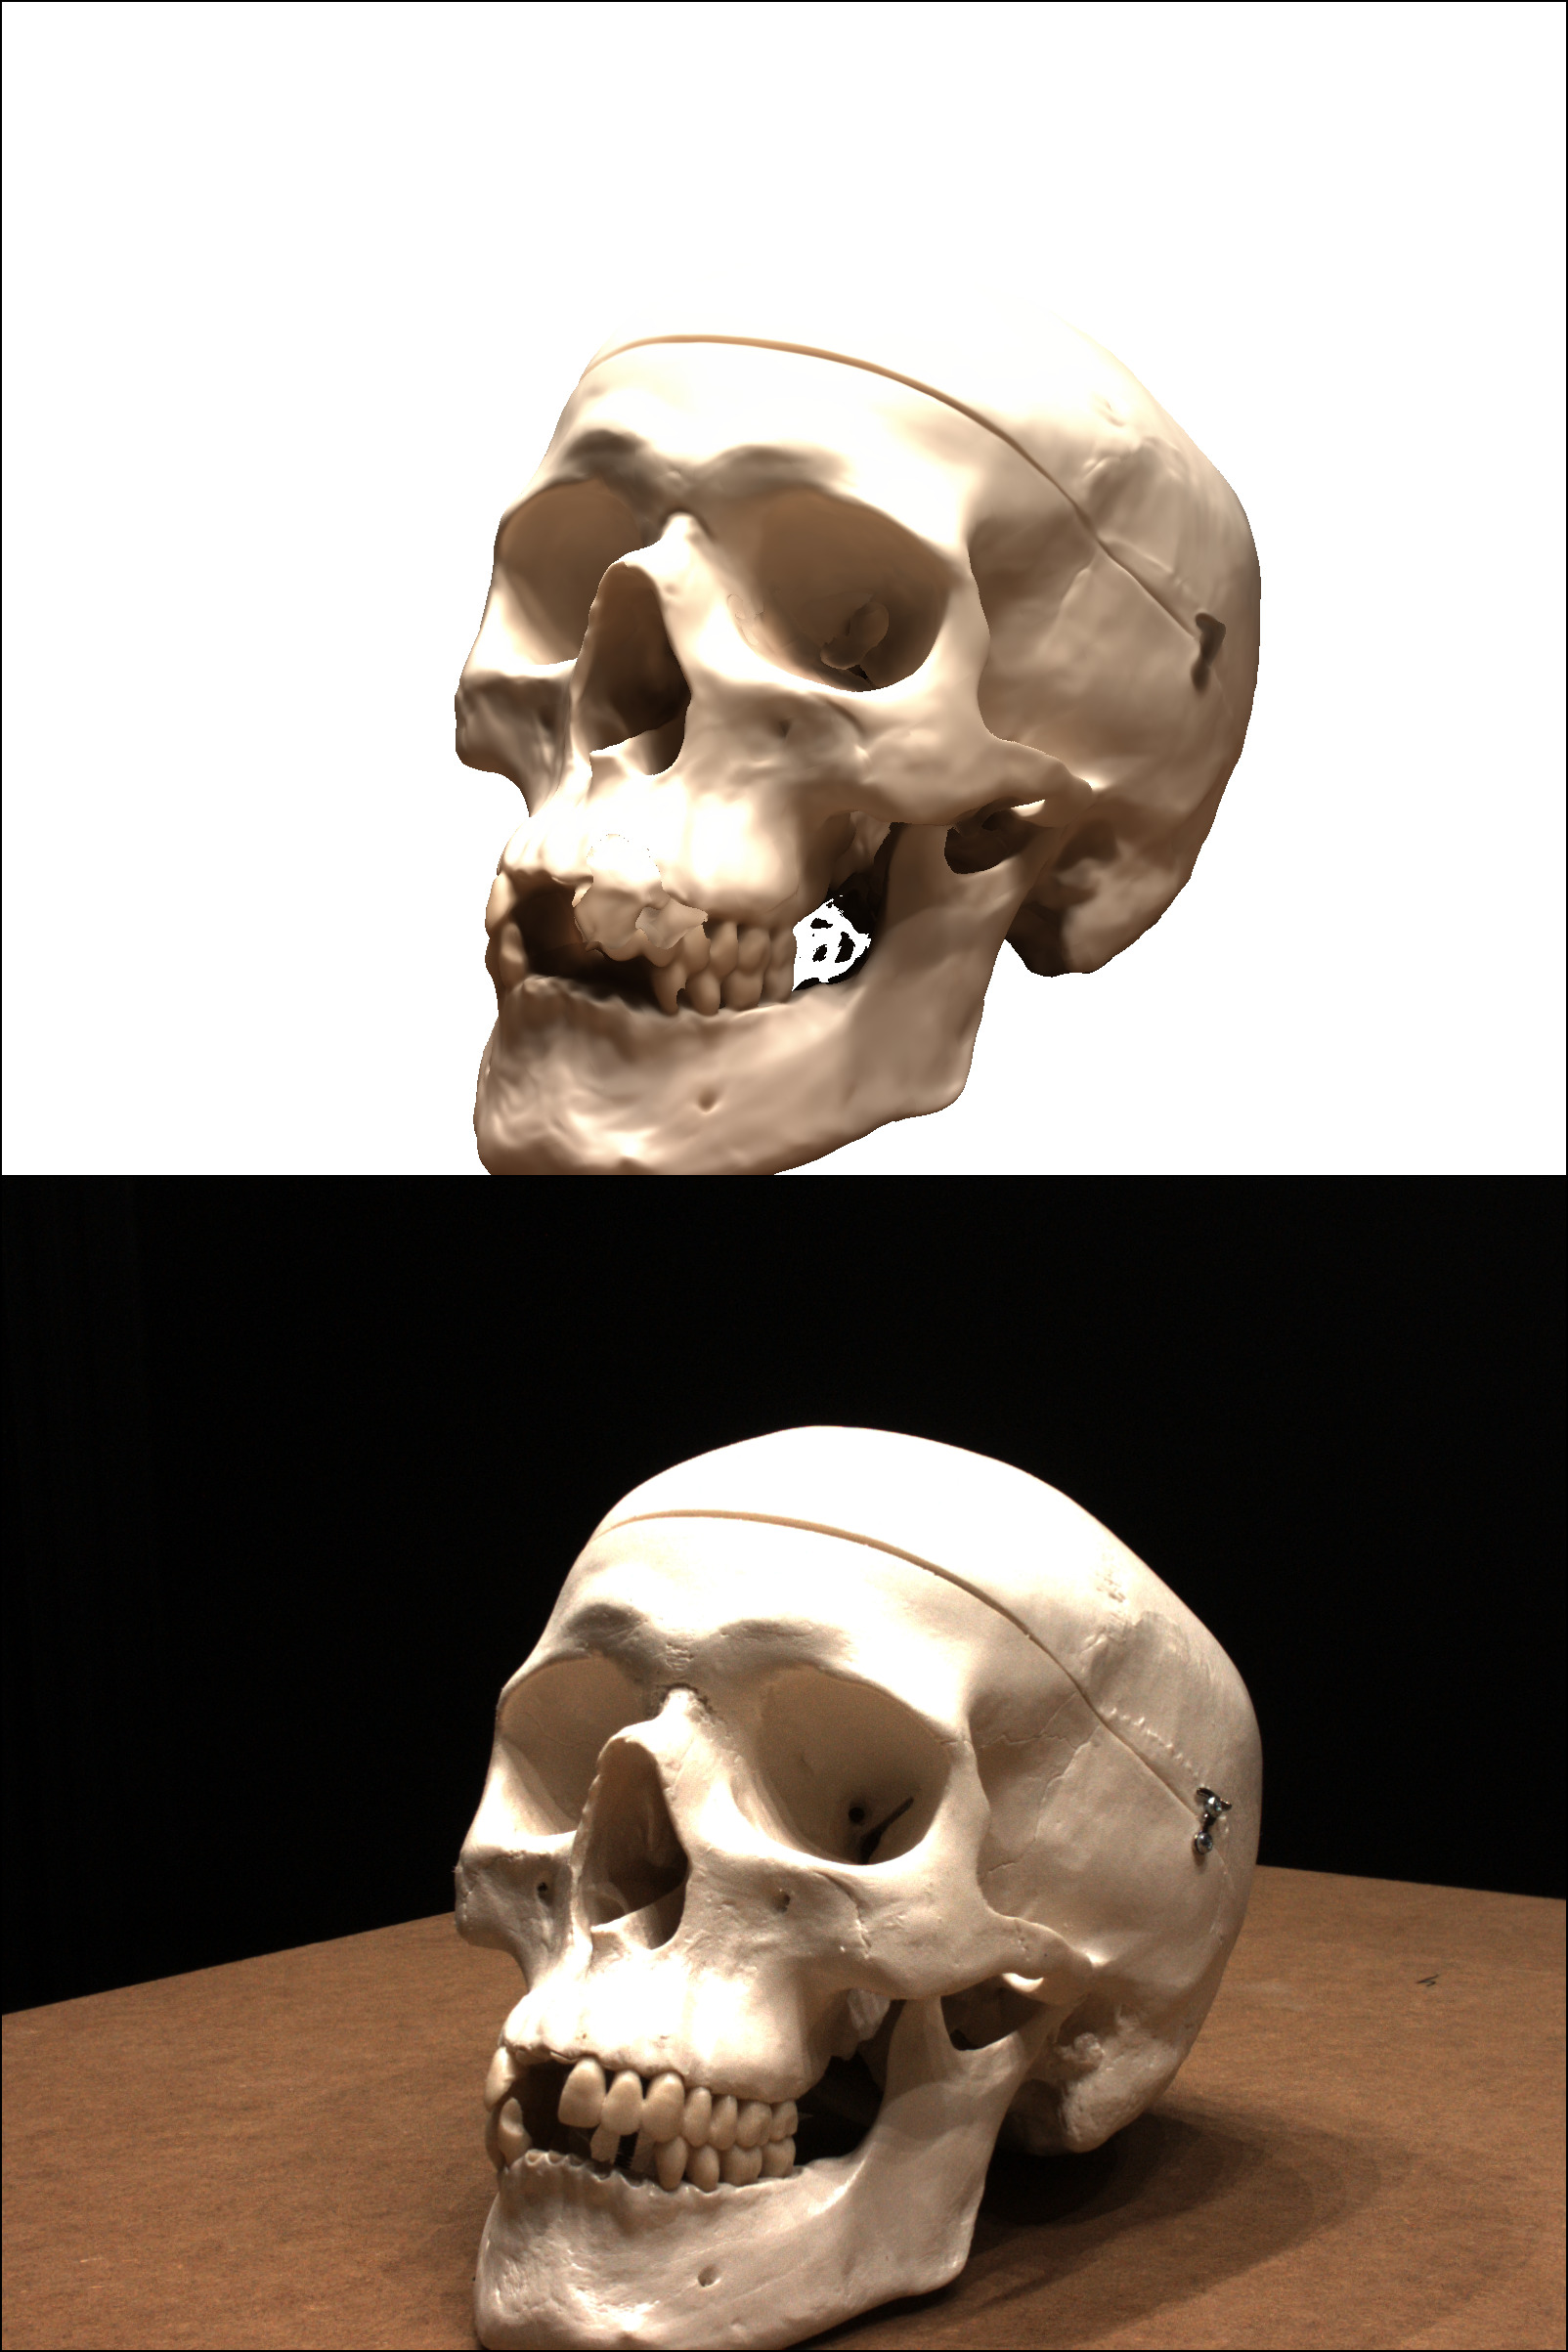
\includegraphics[width=1.5cm]{images/chapter5_img/RenderedImages-DepthMaps-EpochWise-Evals/NFFB/65/rendering_2000.jpg} &  
    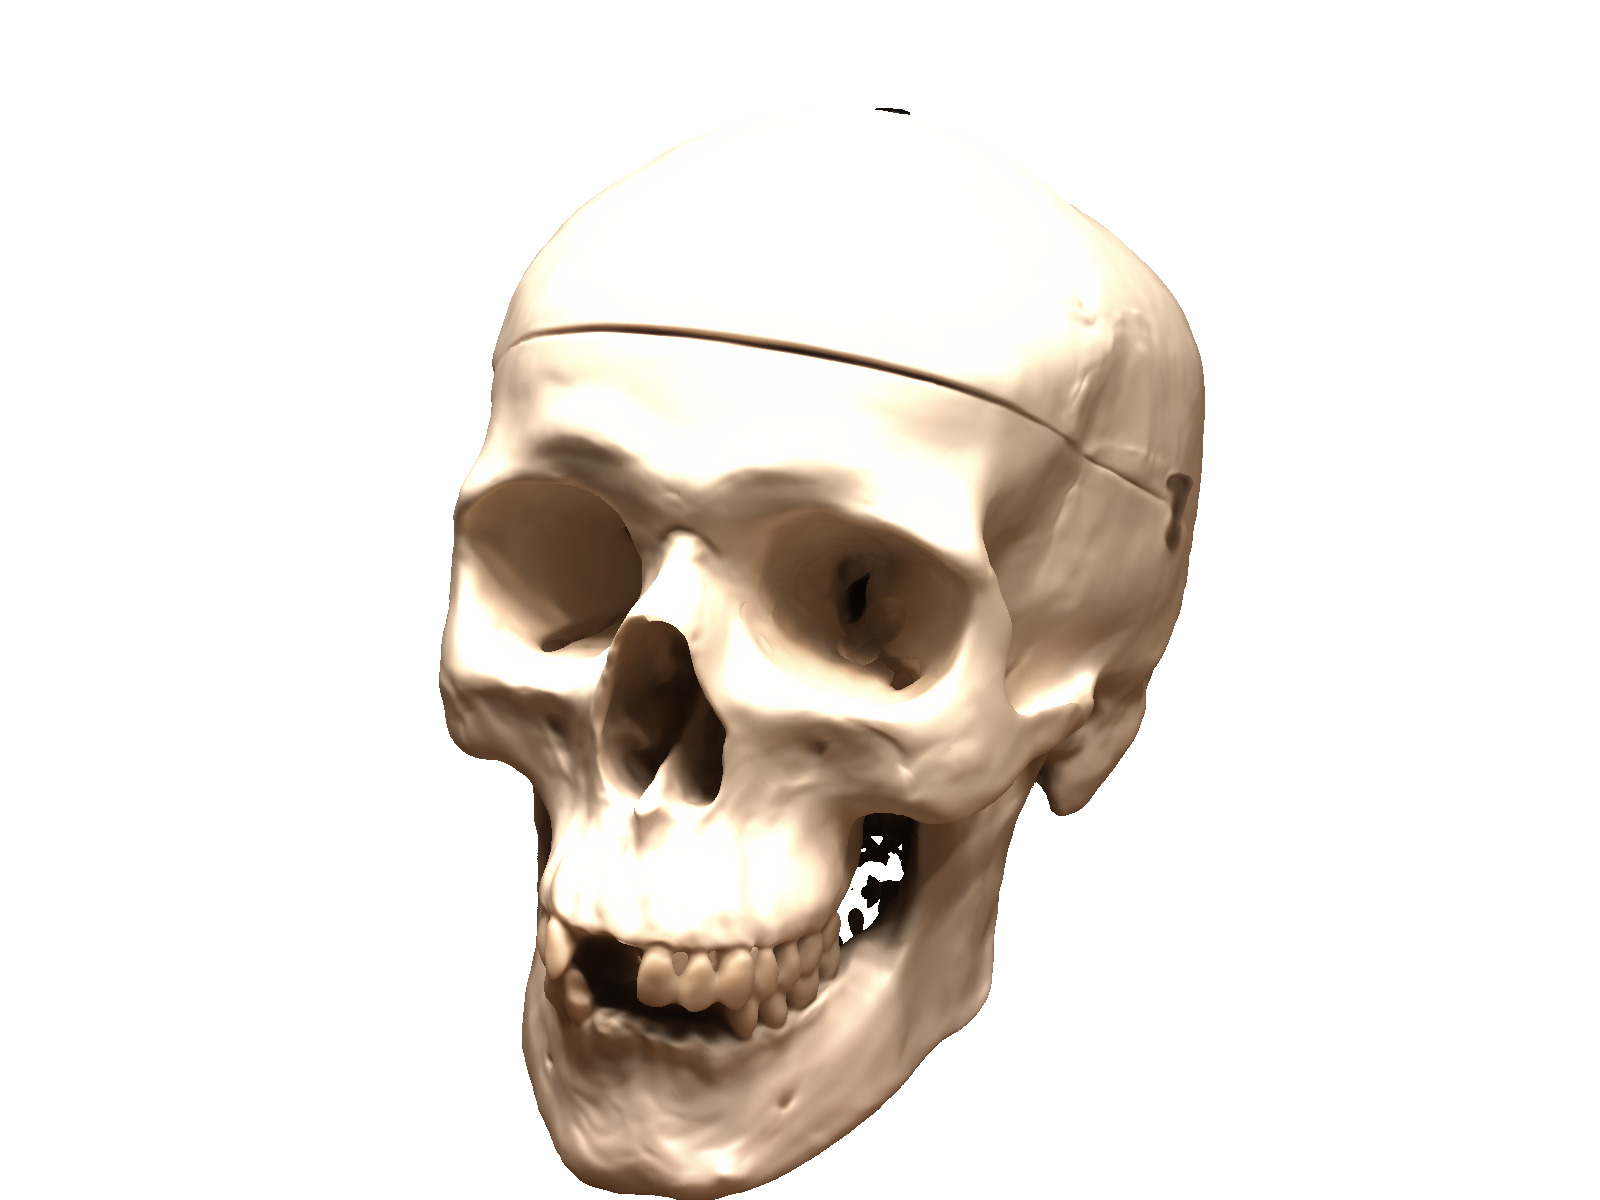
\includegraphics[width=1.5cm]{images/chapter5_img/RenderedImages-DepthMaps-EpochWise-Evals/NFFB/65/eval_035.jpg} \\
    \hline
    StyleMod NFFB & 
    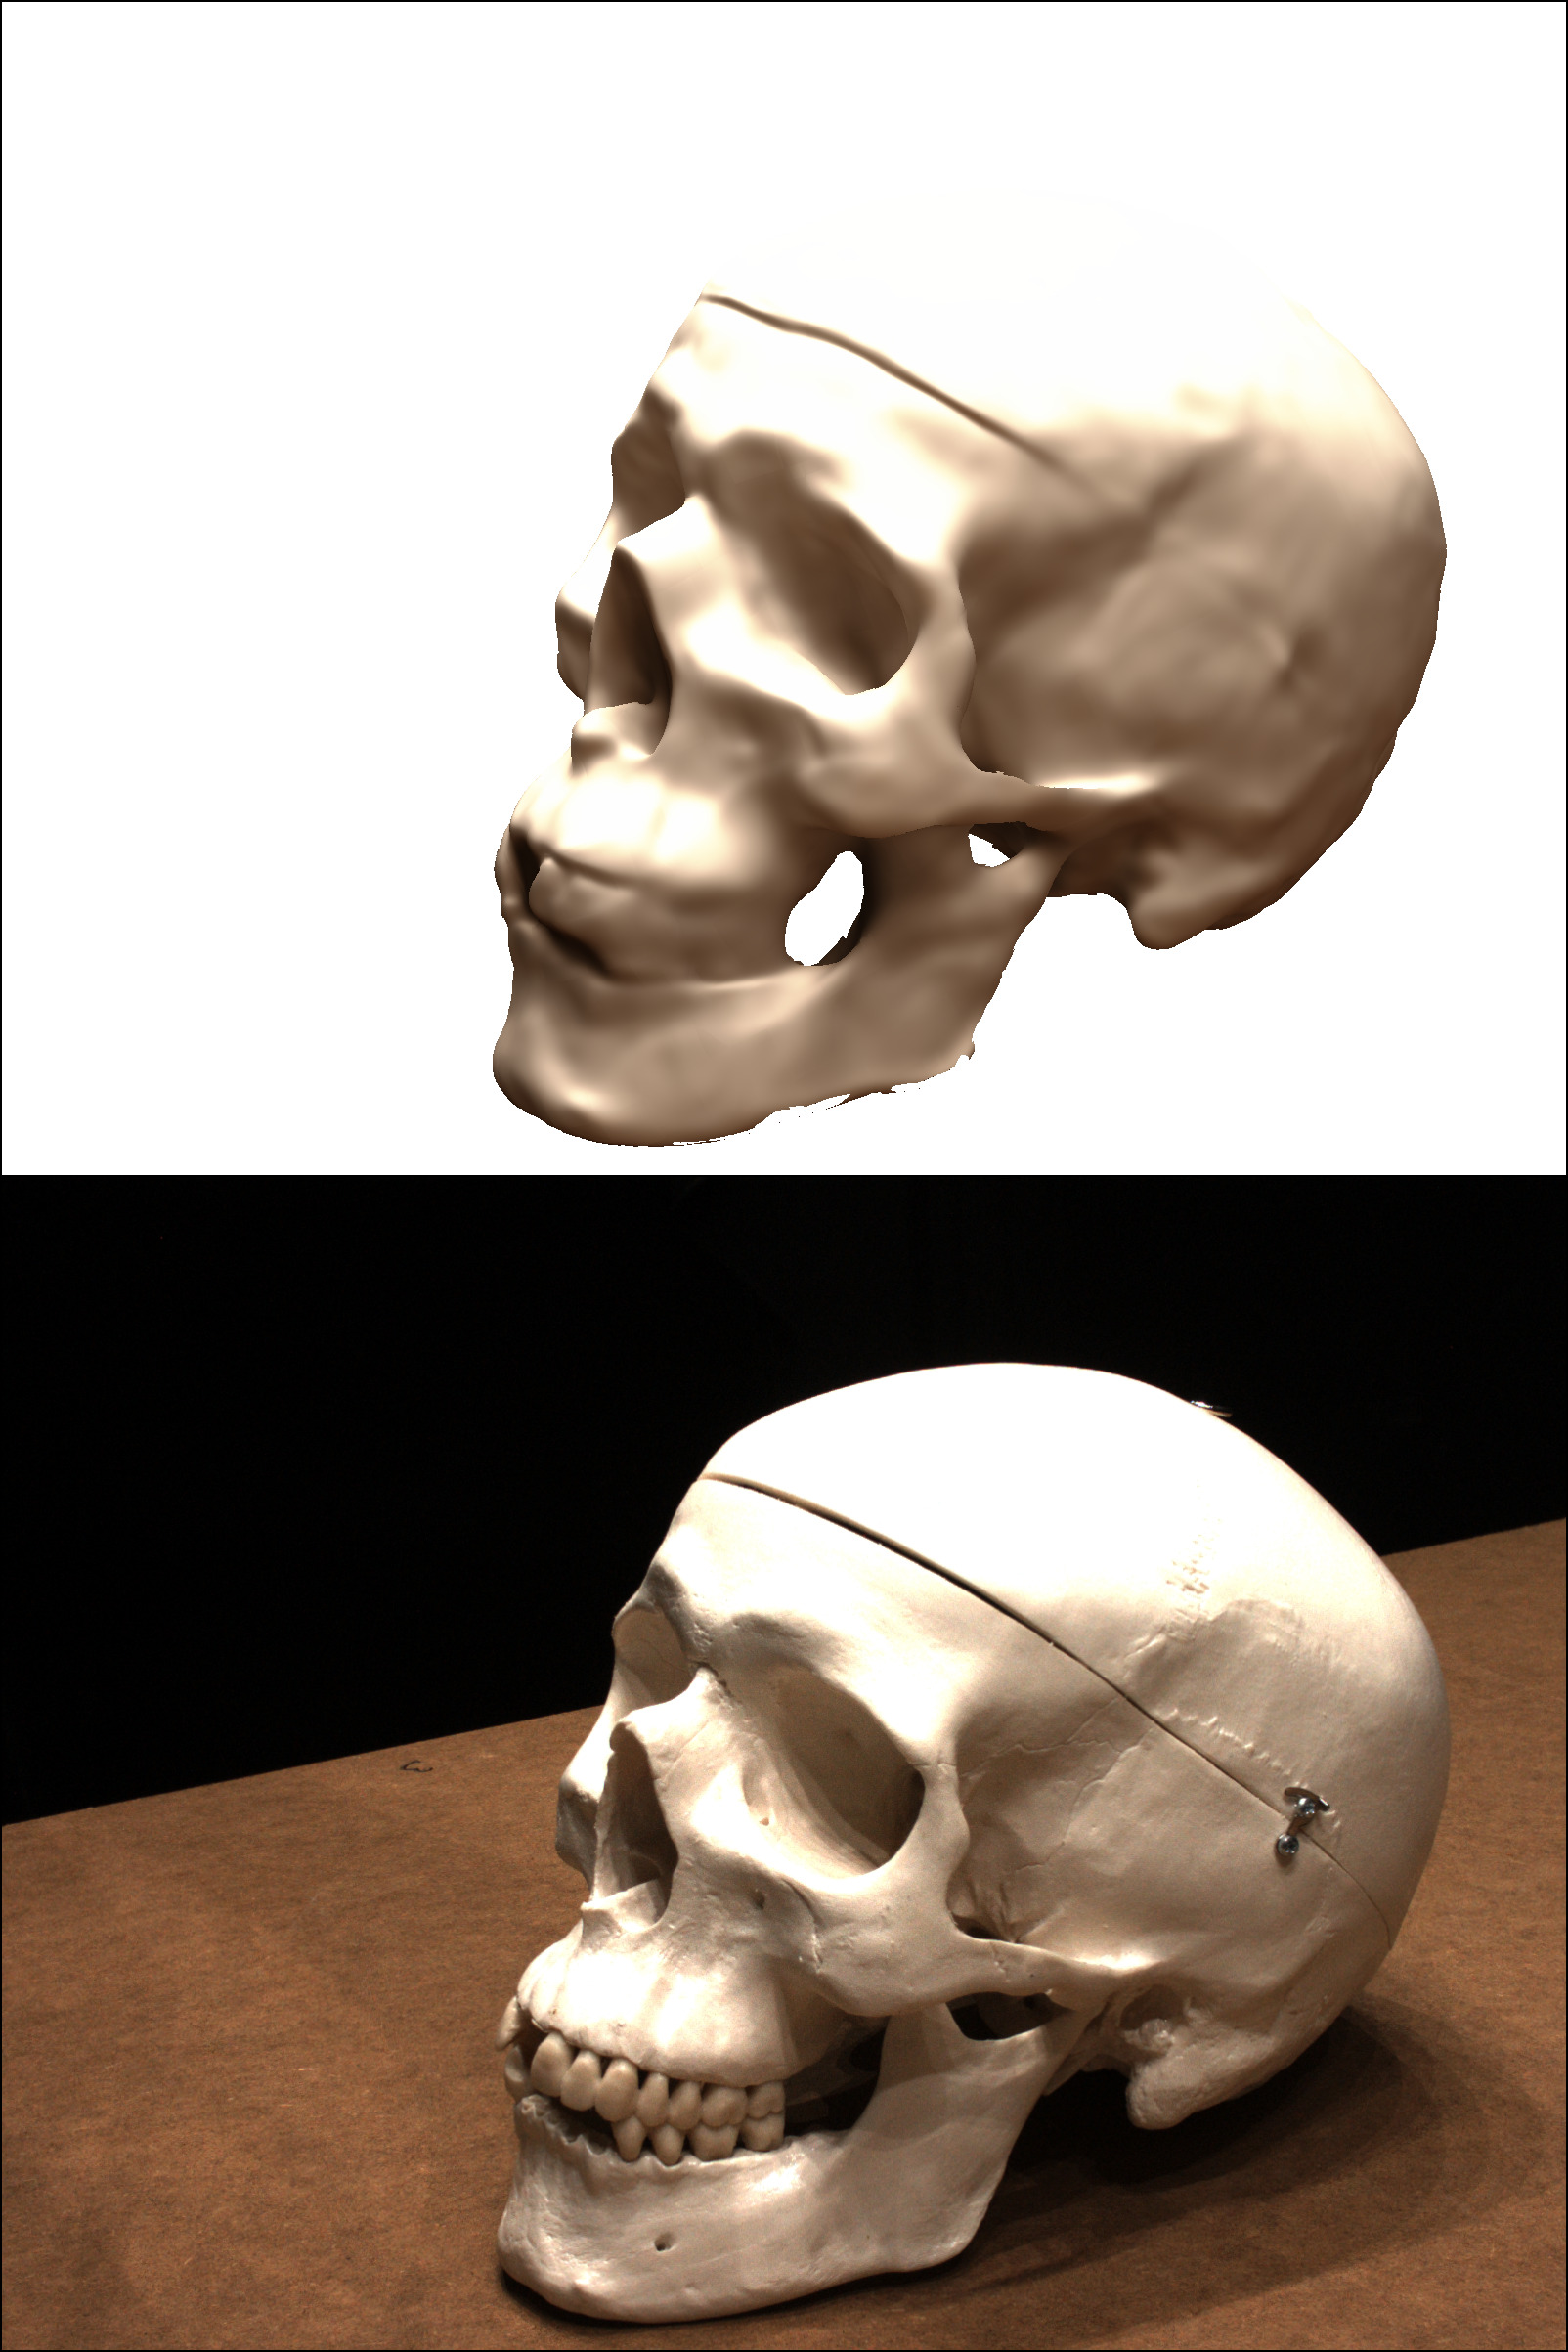
\includegraphics[width=1.5cm]{images/chapter5_img/RenderedImages-DepthMaps-EpochWise-Evals/StylemodNFFB/65/rendering_100.jpg} & 
    \includegraphics[width=1.5cm]{images/chapter5_img/RenderedImages-DepthMaps-EpochWise-Evals/StylemodNFFB/65/rendering_500.jpg} & 
    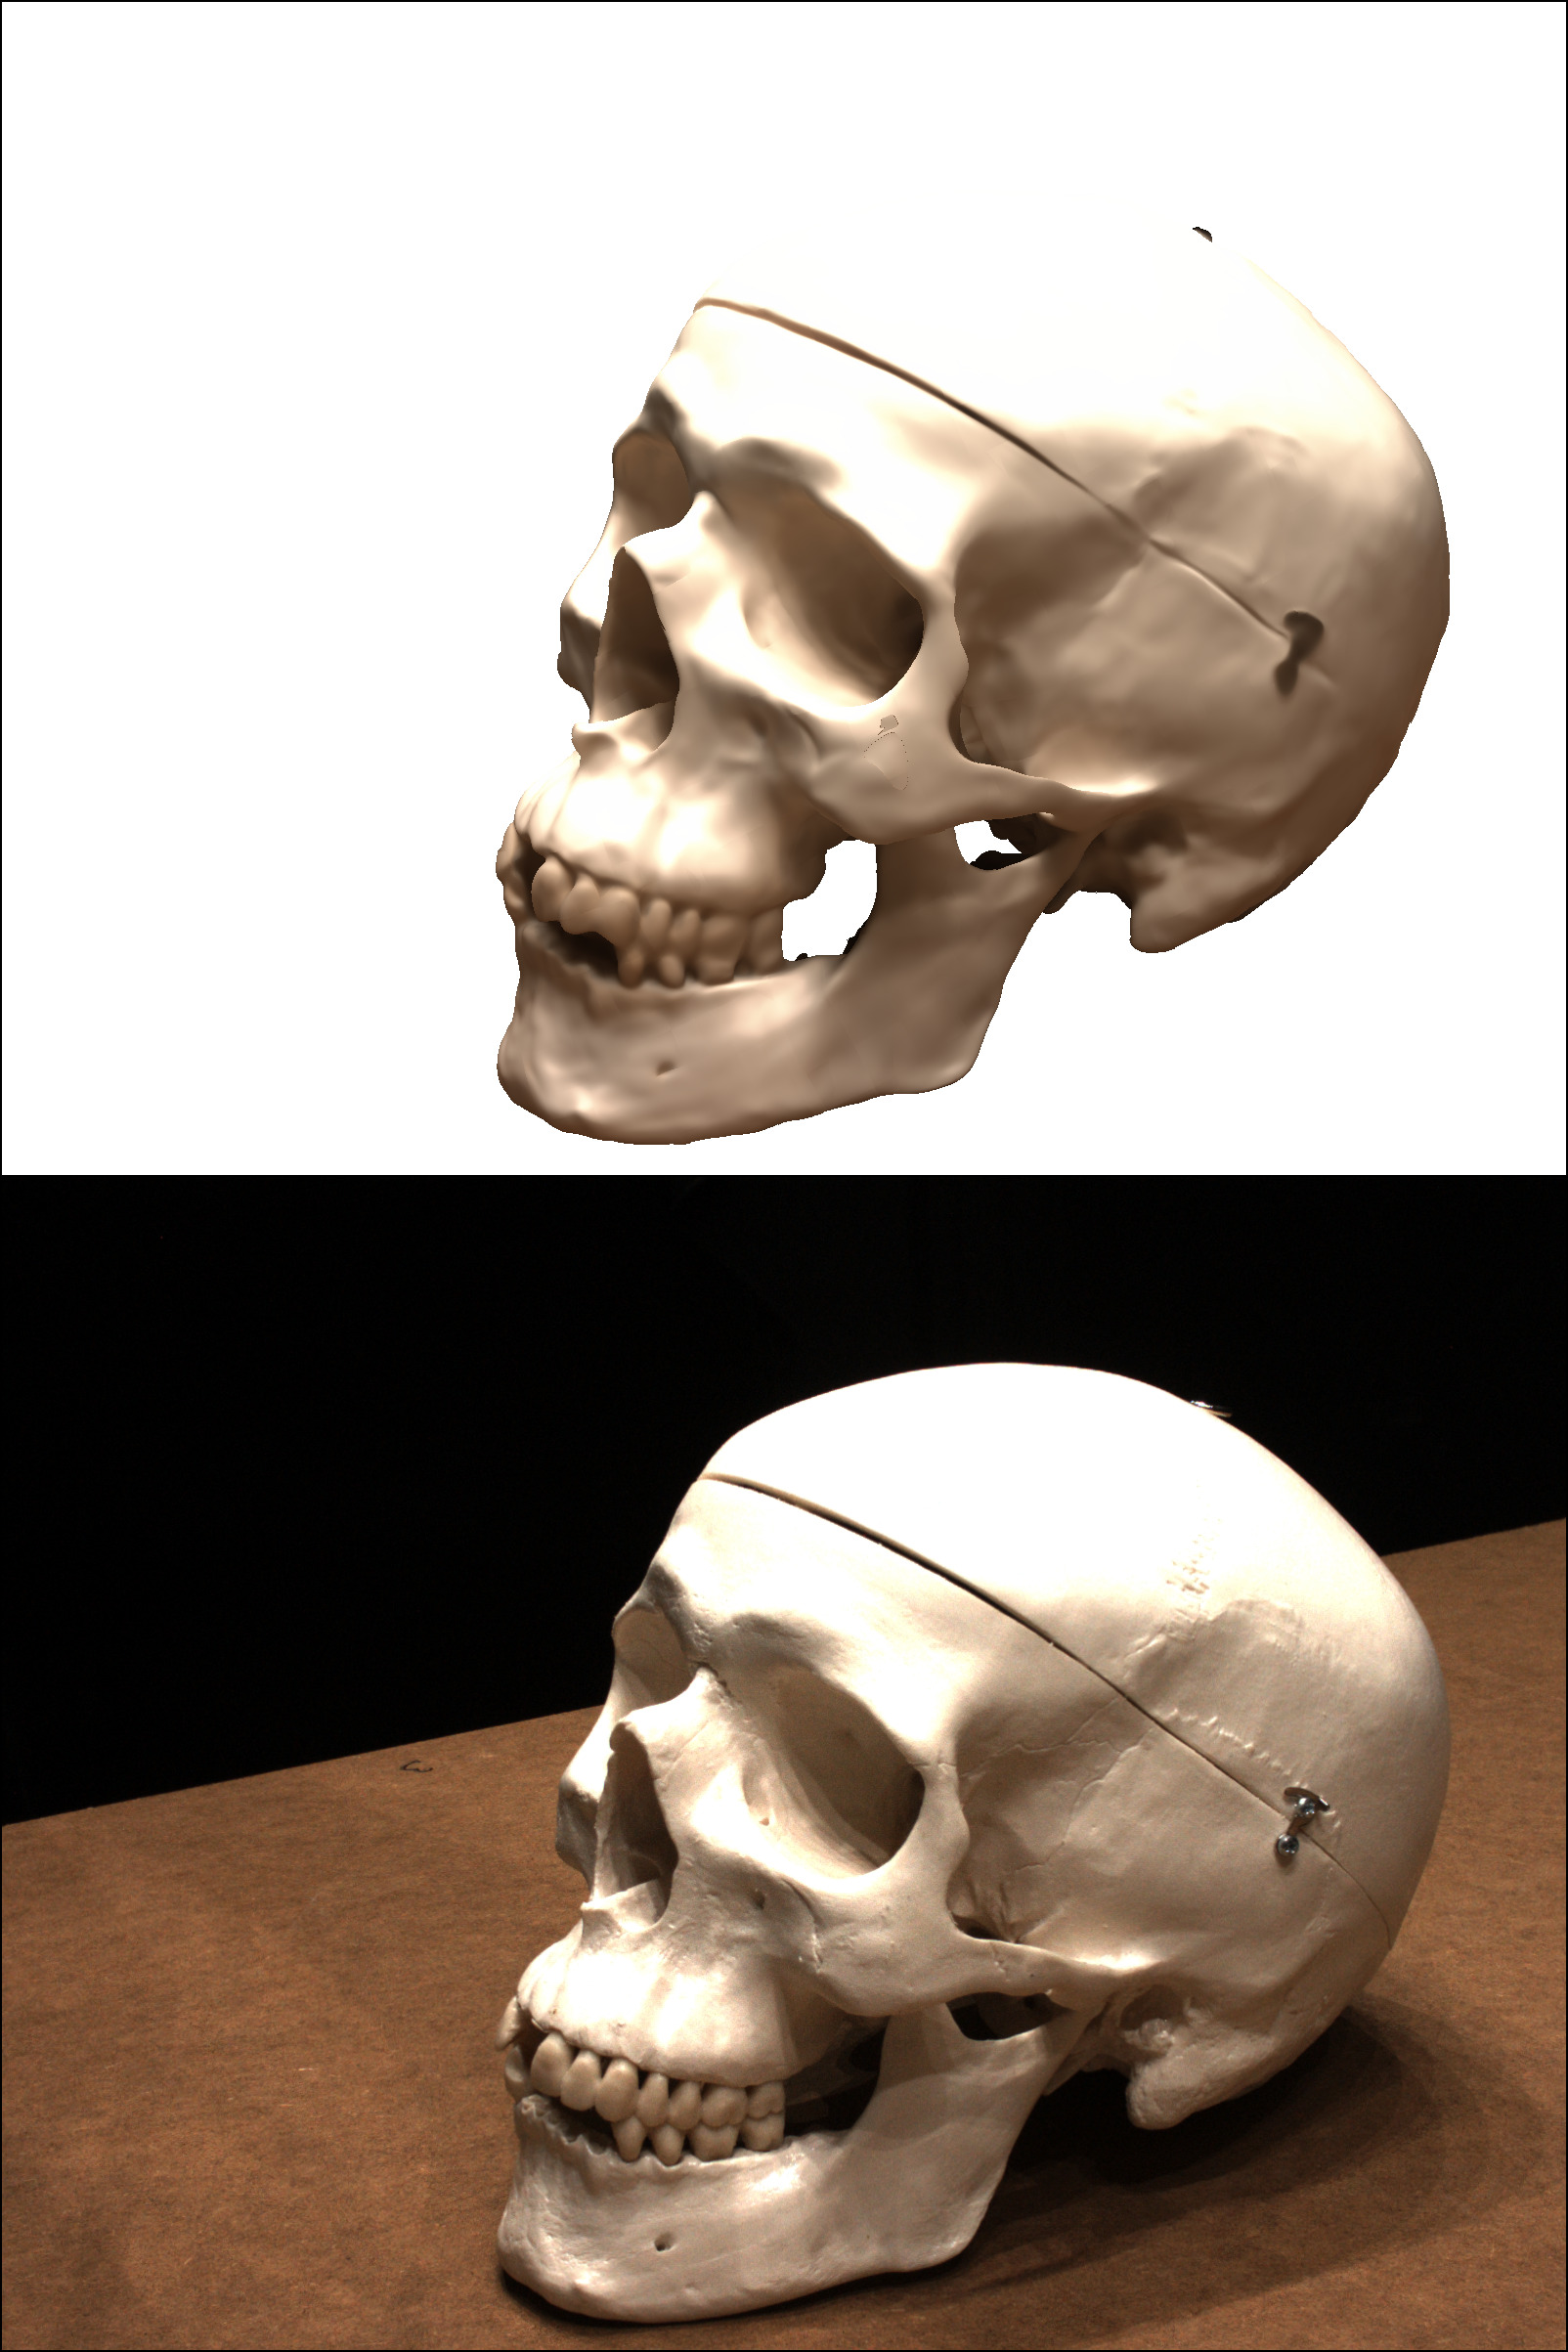
\includegraphics[width=1.5cm]{images/chapter5_img/RenderedImages-DepthMaps-EpochWise-Evals/StylemodNFFB/65/rendering_1000.jpg} & 
    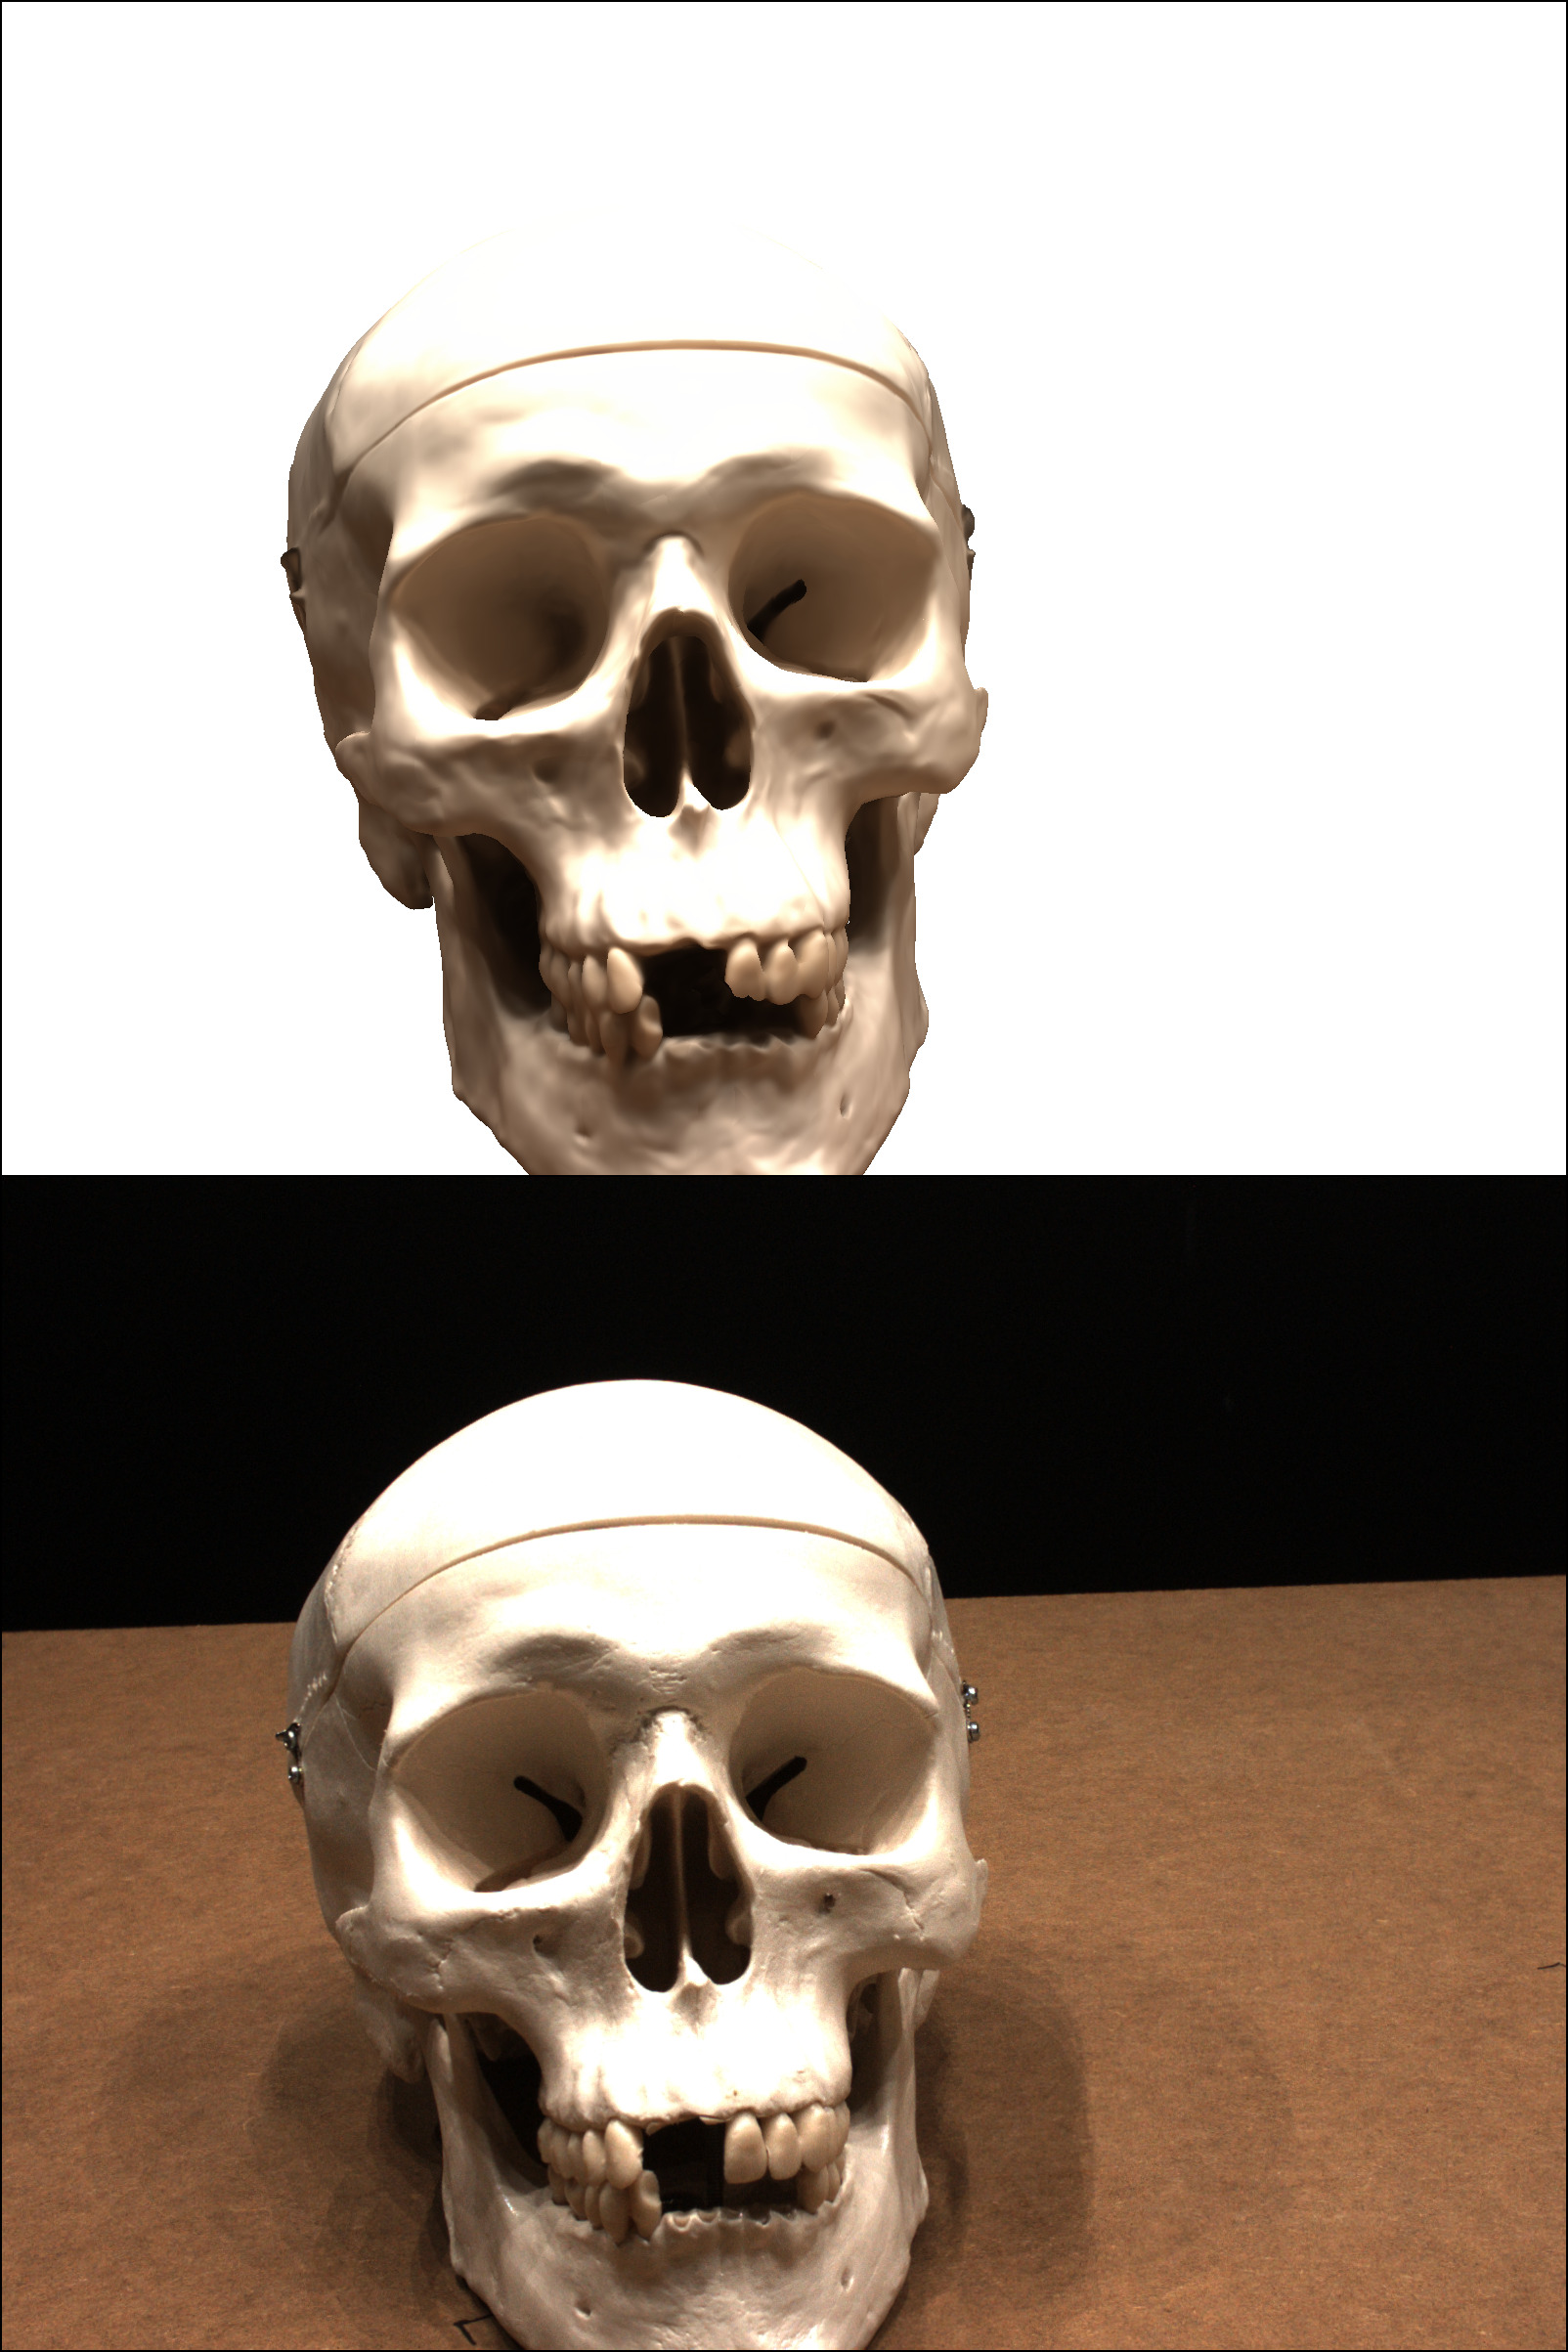
\includegraphics[width=1.5cm]{images/chapter5_img/RenderedImages-DepthMaps-EpochWise-Evals/StylemodNFFB/65/rendering_2000.jpg} & 
    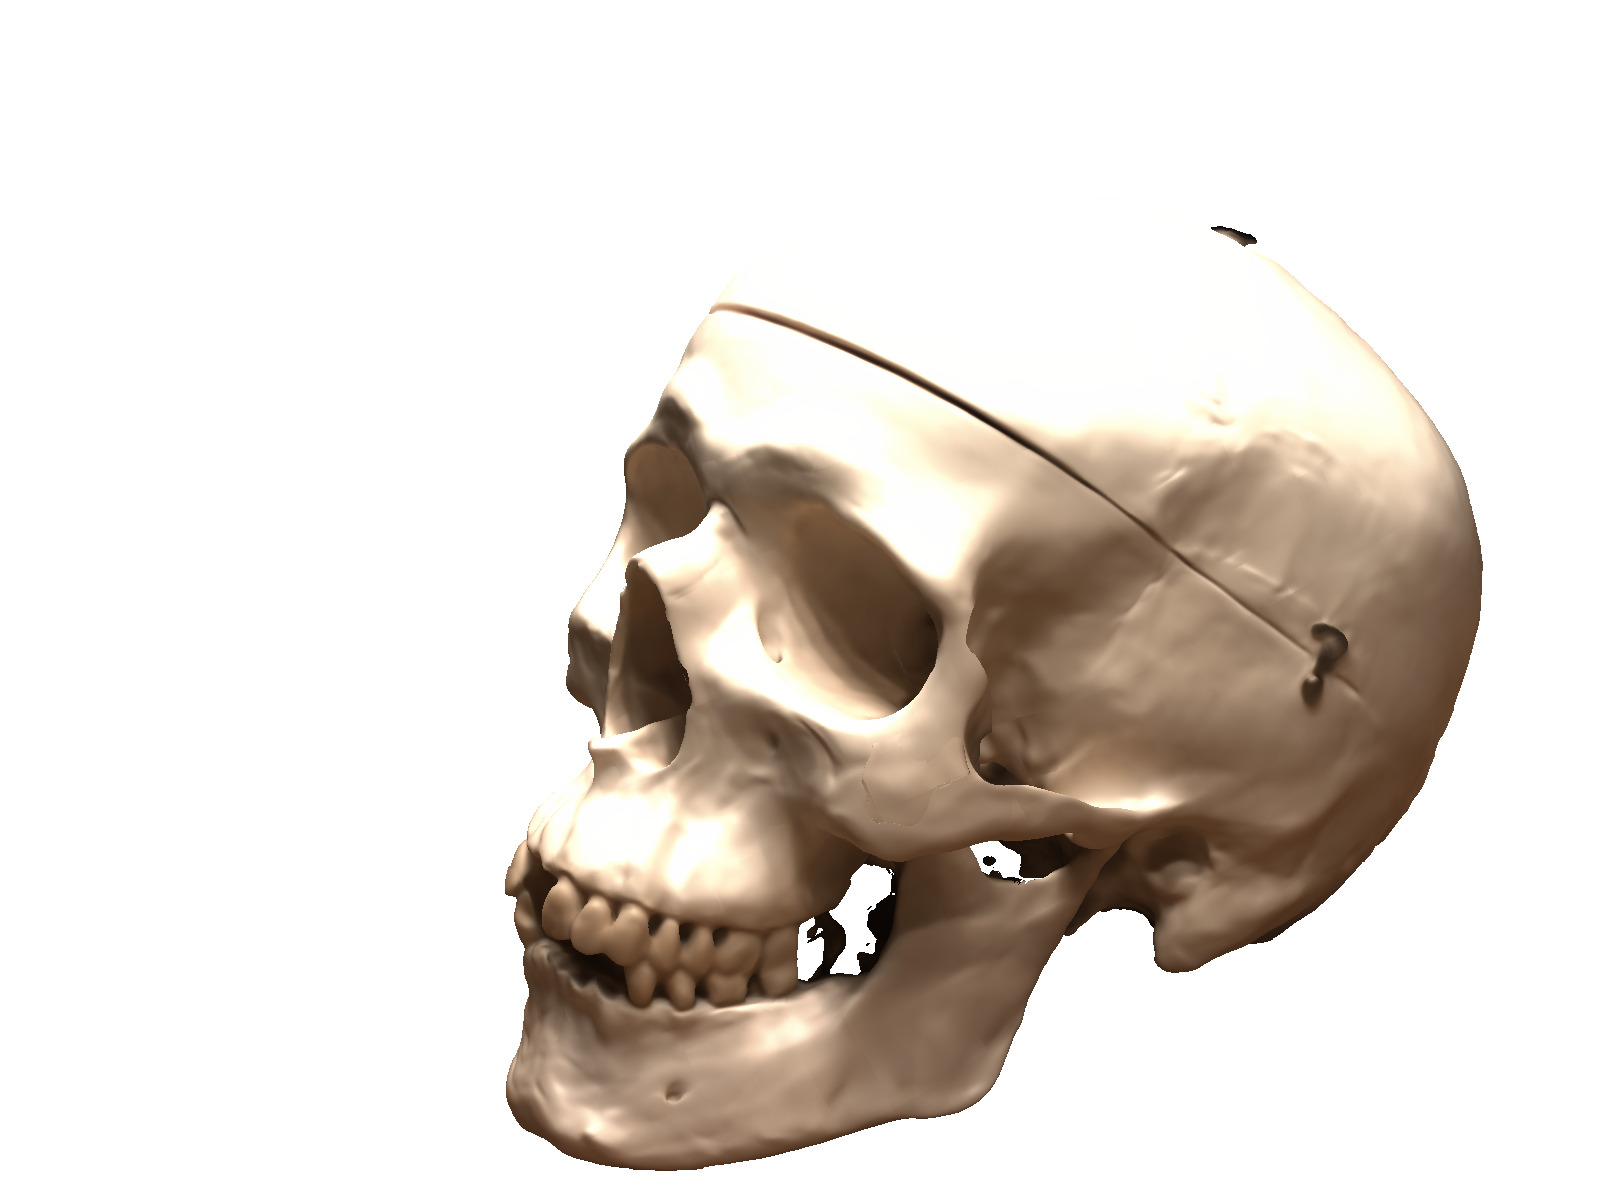
\includegraphics[width=1.5cm]{images/chapter5_img/RenderedImages-DepthMaps-EpochWise-Evals/StylemodNFFB/65/eval_035.jpg} \\
    \hline
    StyleModNFFB (TinyCudaNN) & 
    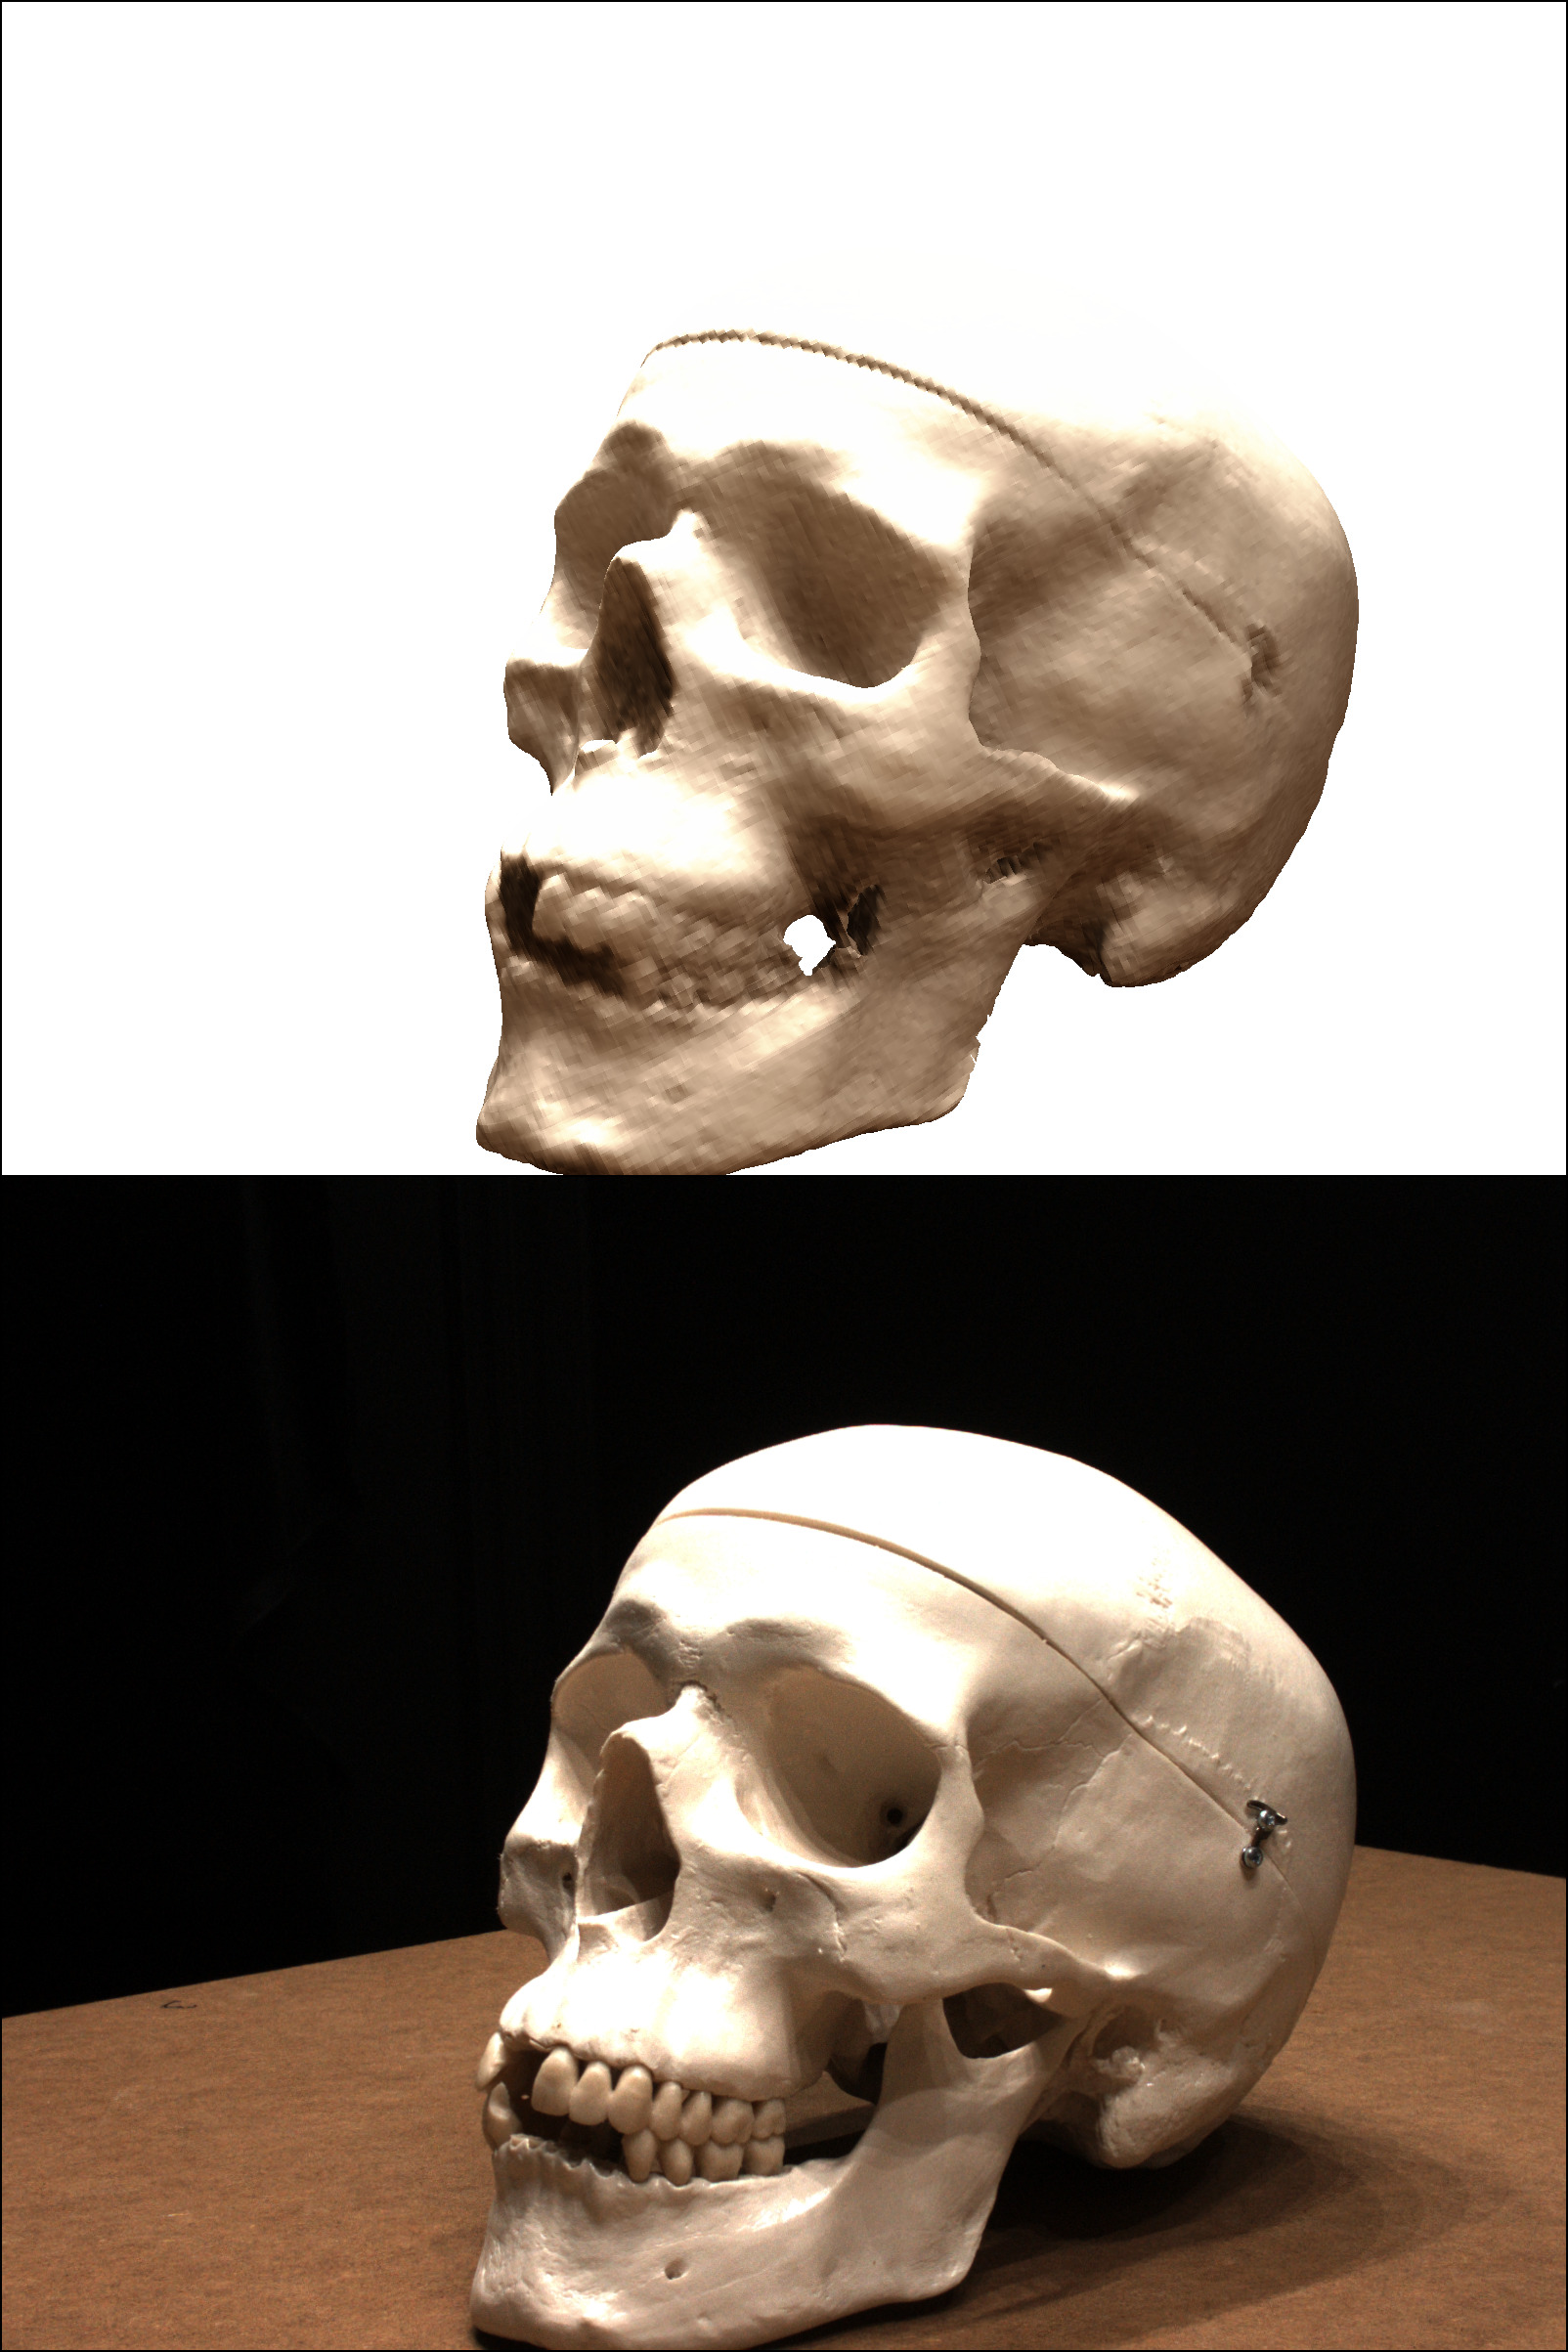
\includegraphics[width=1.5cm]{images/chapter5_img/RenderedImages-DepthMaps-EpochWise-Evals/StylemodNFFB_TCNN/65/rendering_100.jpg} & 
    \includegraphics[width=1.5cm]{images/chapter5_img/RenderedImages-DepthMaps-EpochWise-Evals/StylemodNFFB_TCNN/65/rendering_500.jpg} & 
    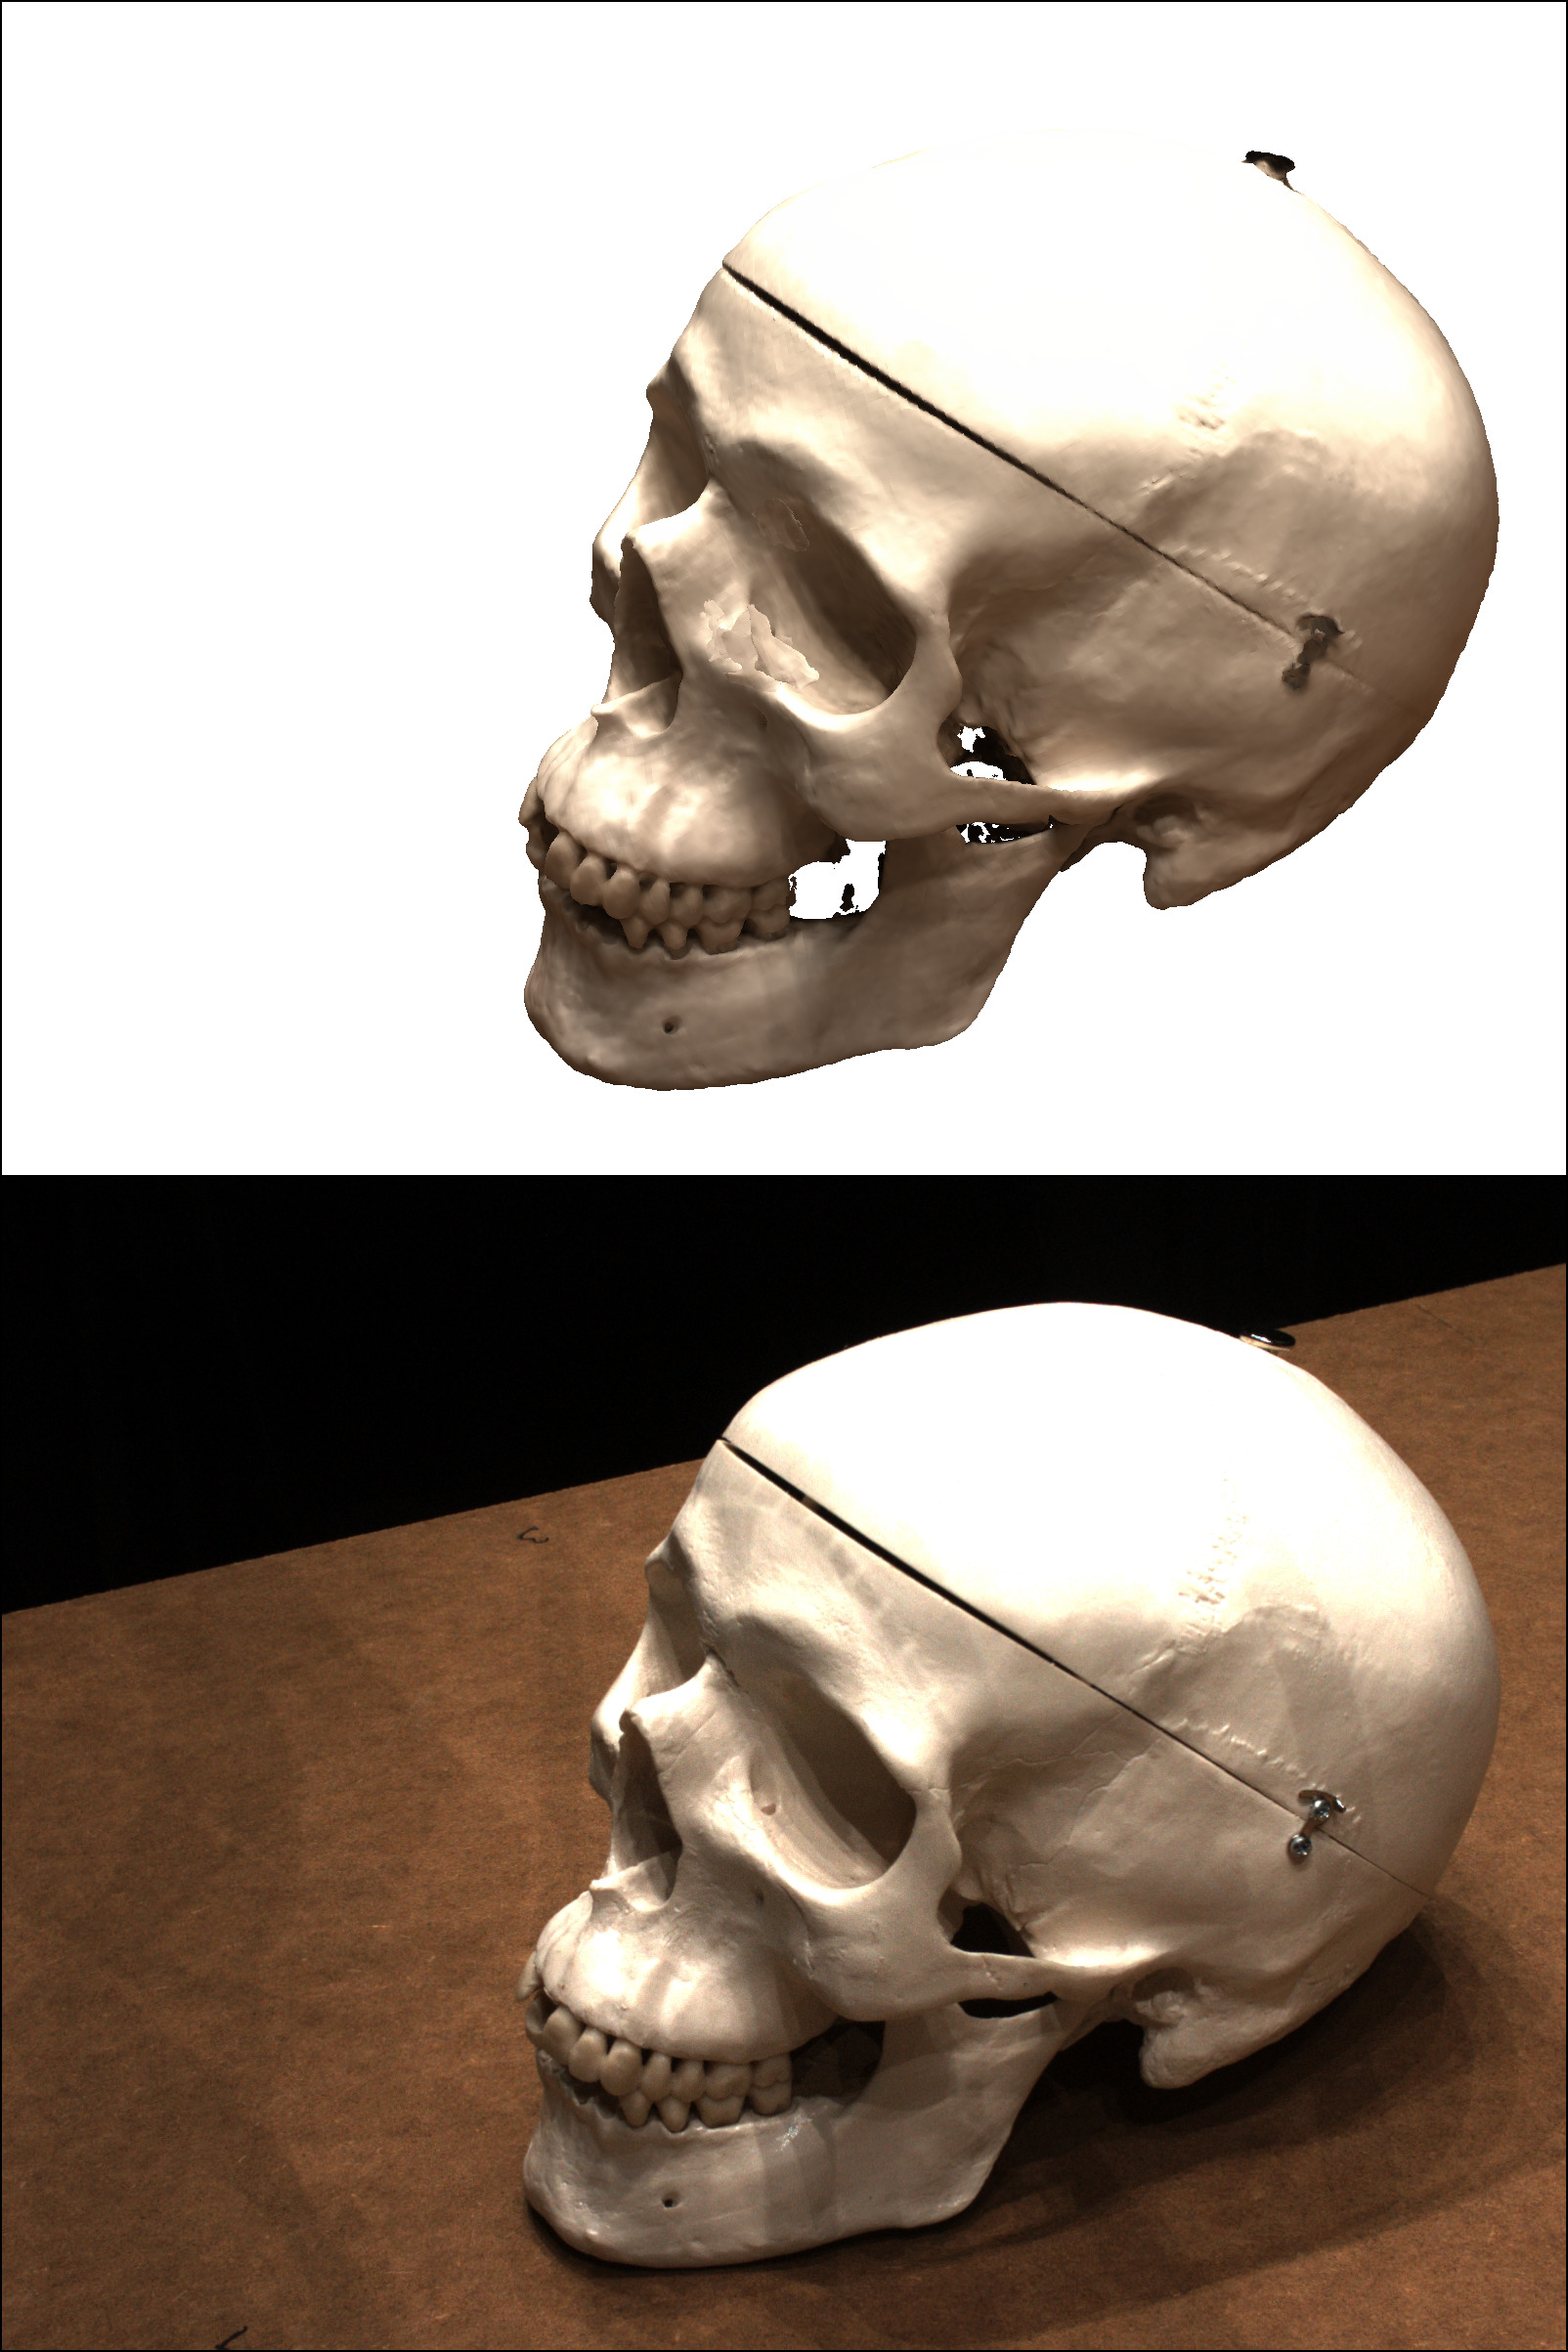
\includegraphics[width=1.5cm]{images/chapter5_img/RenderedImages-DepthMaps-EpochWise-Evals/StylemodNFFB_TCNN/65/rendering_1000.jpg} & 
    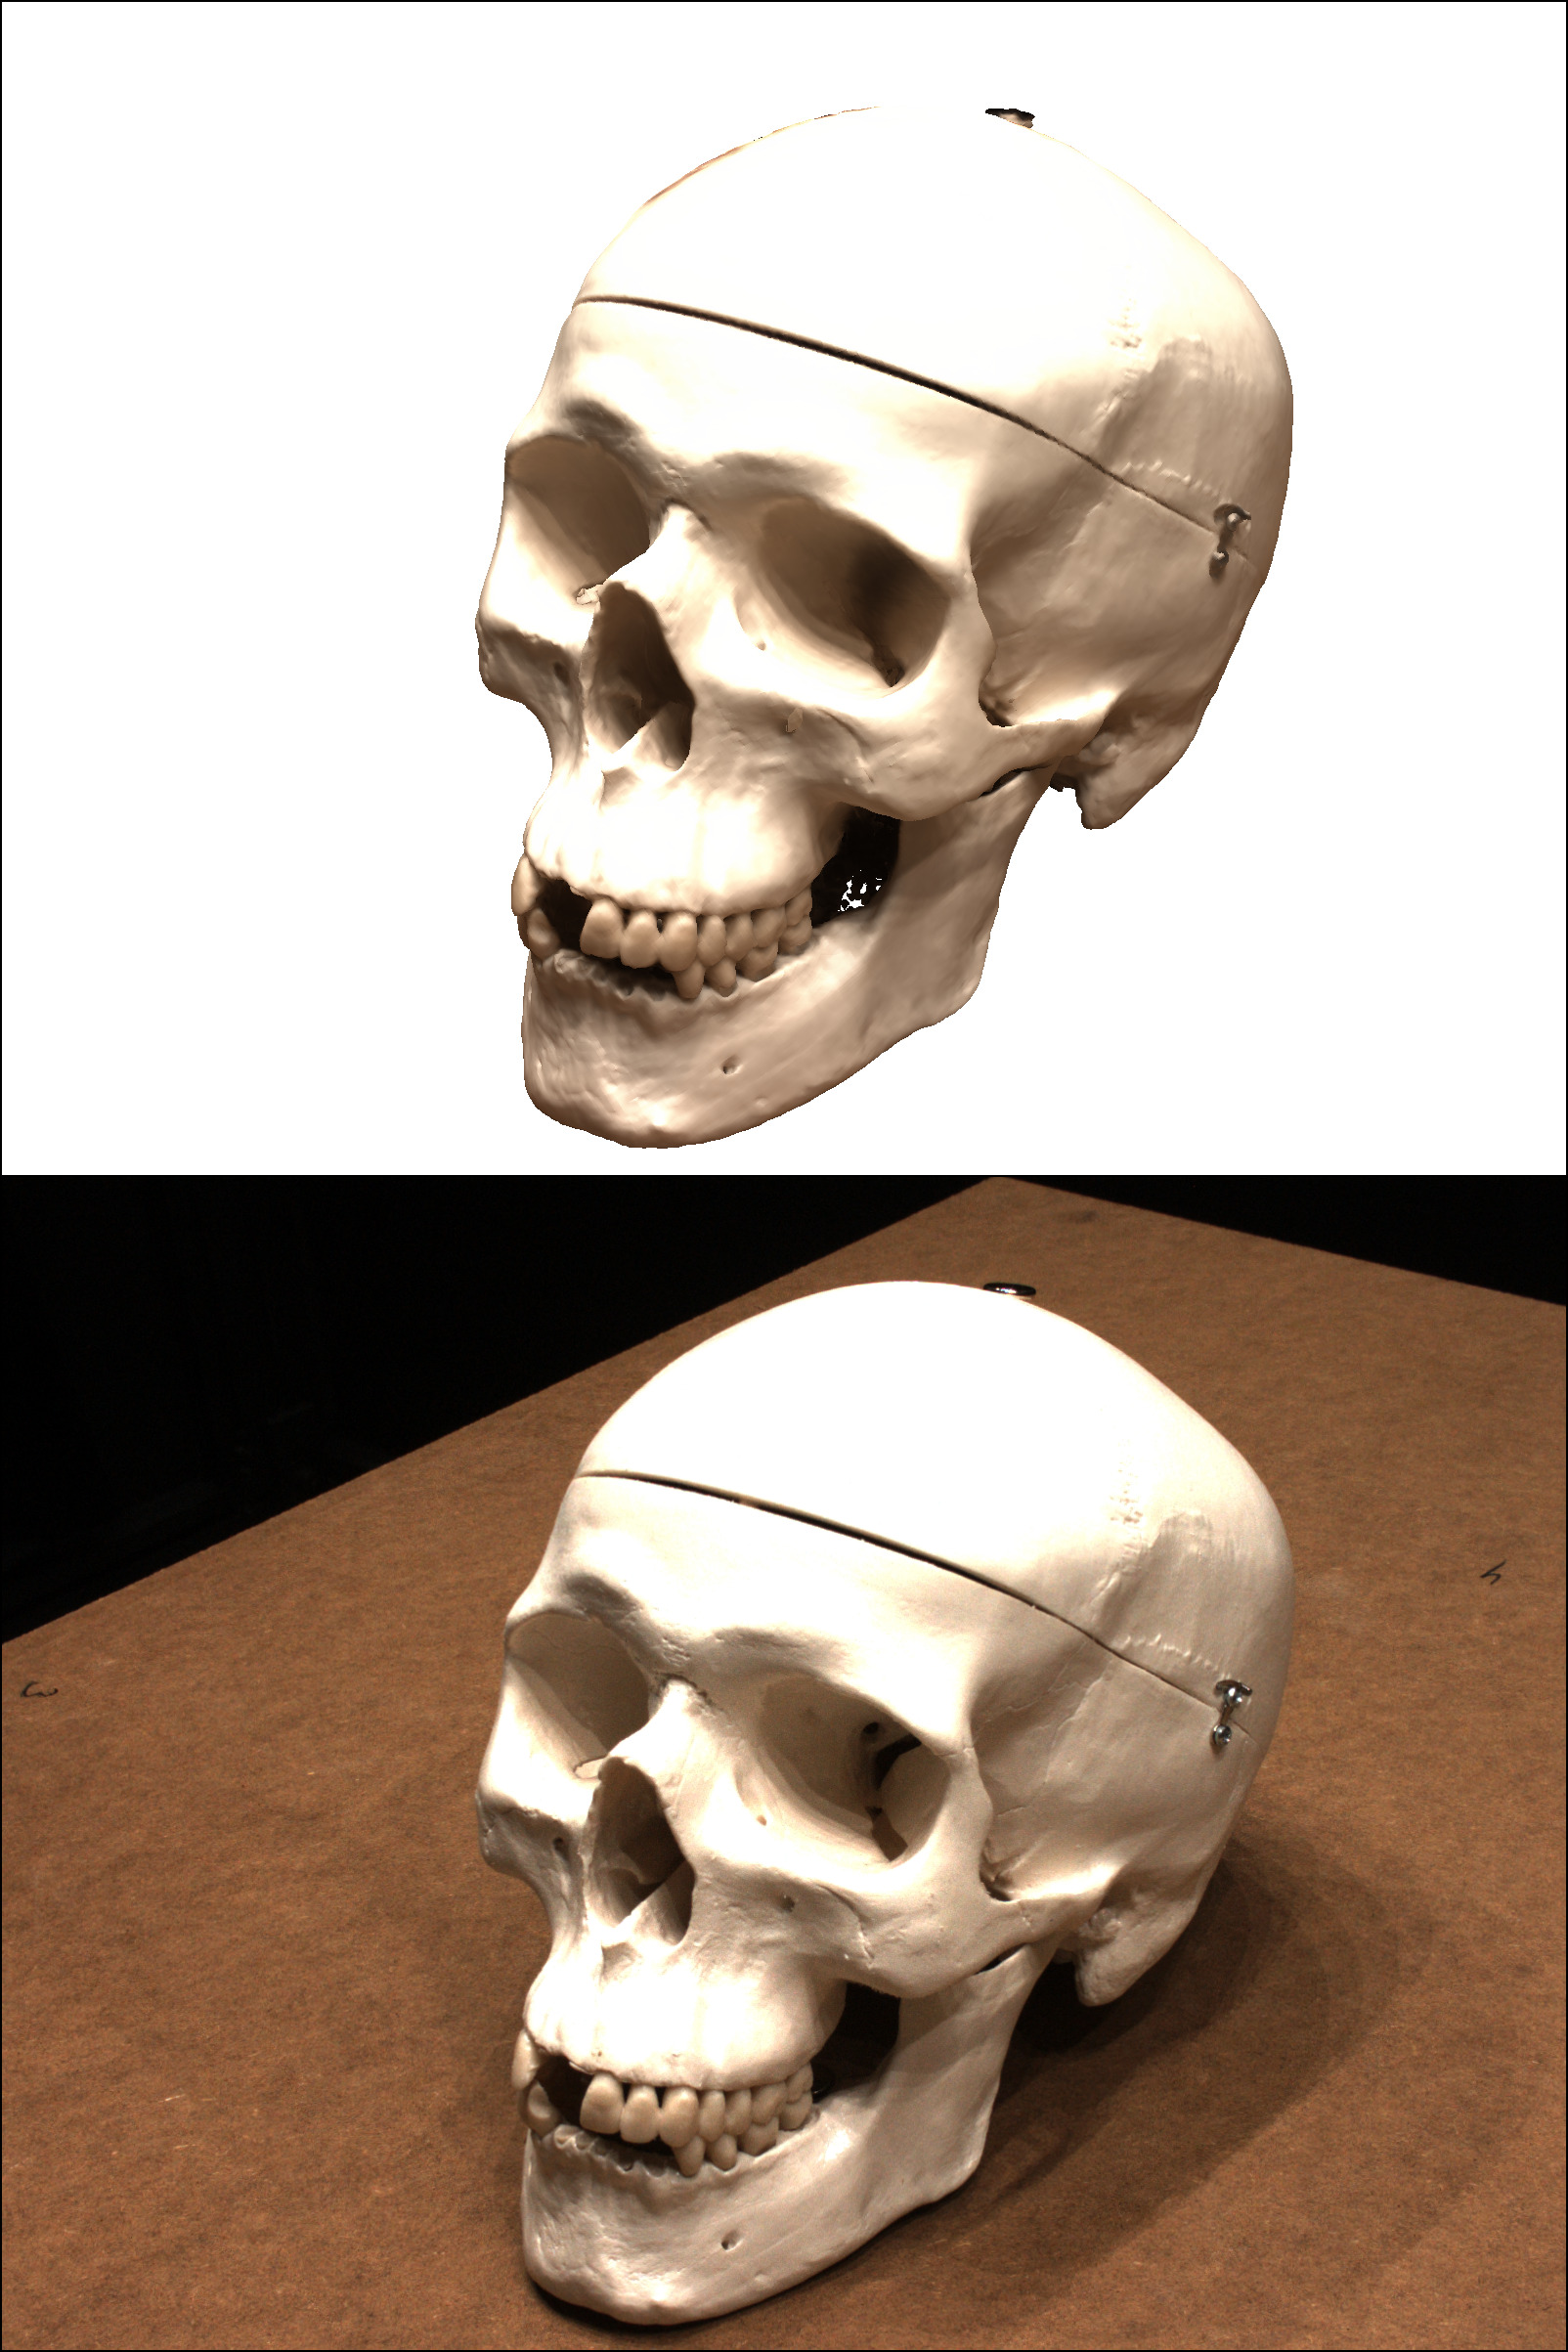
\includegraphics[width=1.5cm]{images/chapter5_img/RenderedImages-DepthMaps-EpochWise-Evals/StylemodNFFB_TCNN/65/rendering_2000.jpg} & 
    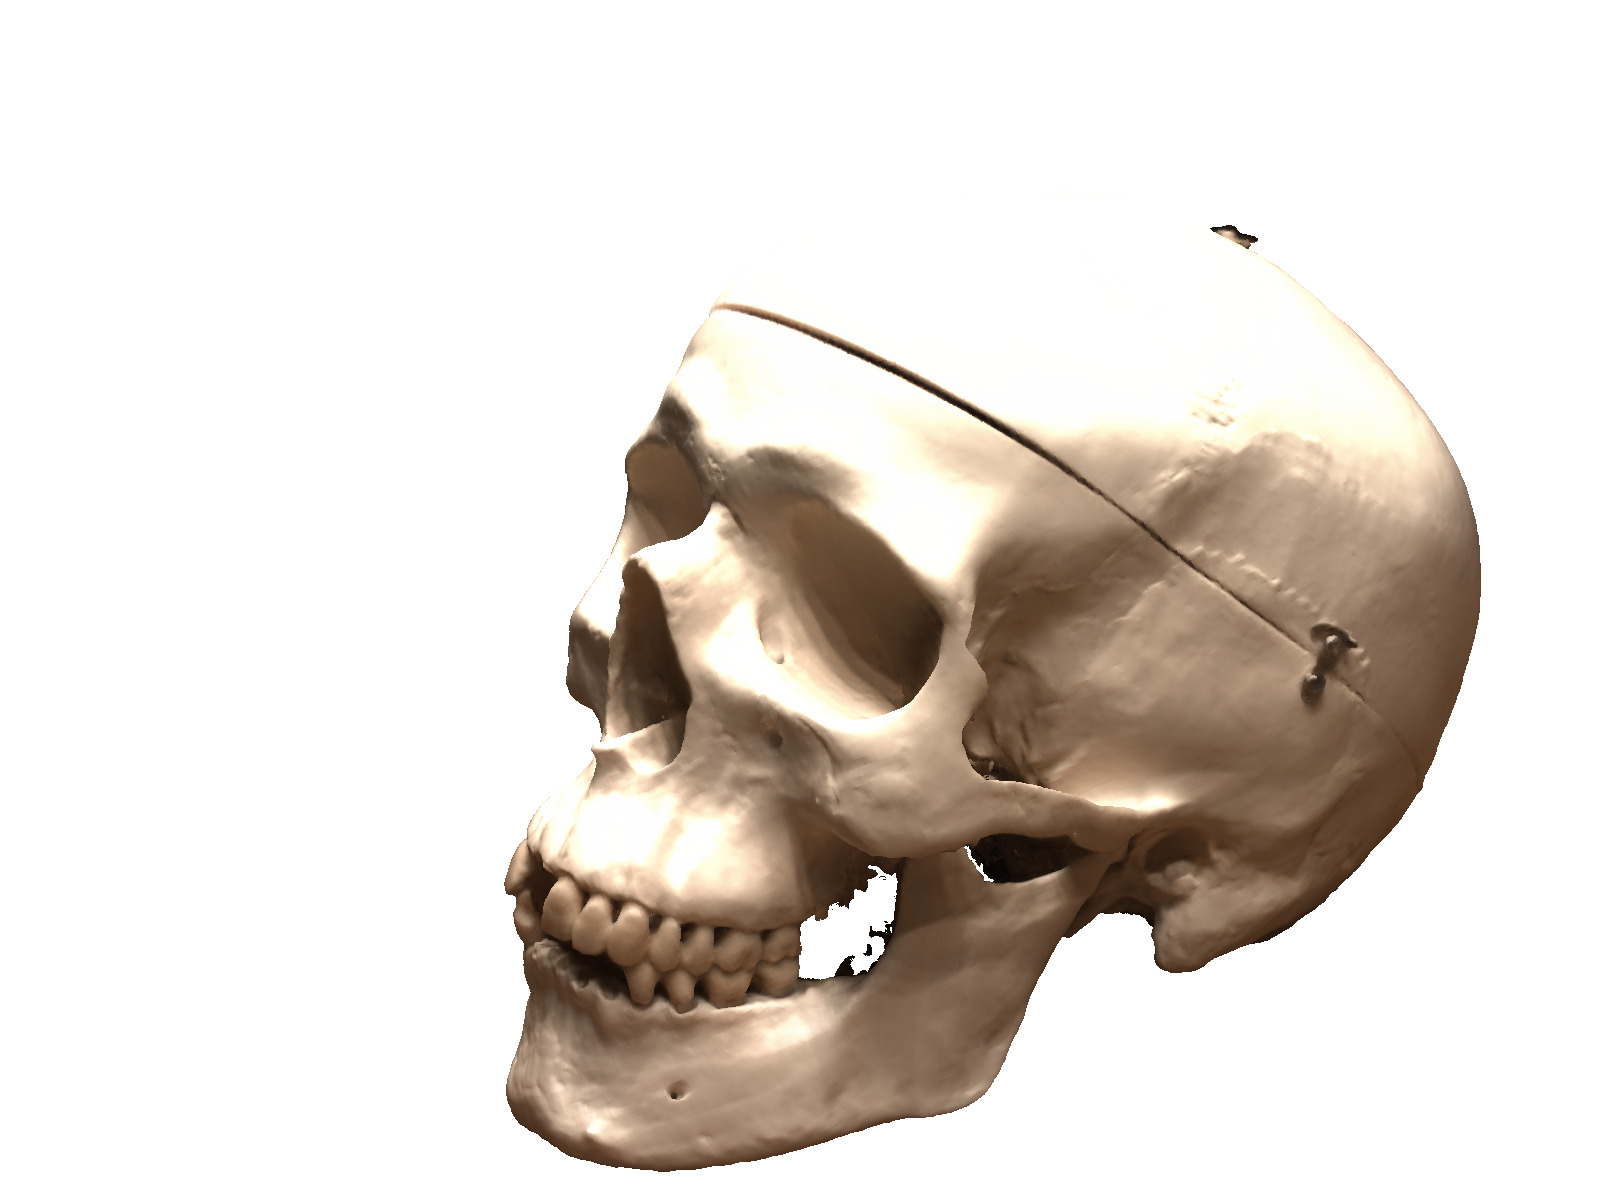
\includegraphics[width=1.5cm]{images/chapter5_img/RenderedImages-DepthMaps-EpochWise-Evals/StylemodNFFB_TCNN/65/eval_035.jpg} \\
    \hline
    
    \end{tabular}
    \caption{Αποτελέσματα 3D Ανακατασκευής Σκηνής 65}
    \end{table}
    \clearpage
\begin{table}[H]
    \centering
    \begin{tabular}{|c|*{6}{p{1.6cm}|}}
    \hline
    Αλγόριθμος & Epoch 100 & Epoch 500 & Epoch 1000 & Epoch 2000 & Eval Πόζα 55 \\
    \hline
    Positional Encoding & 
    % 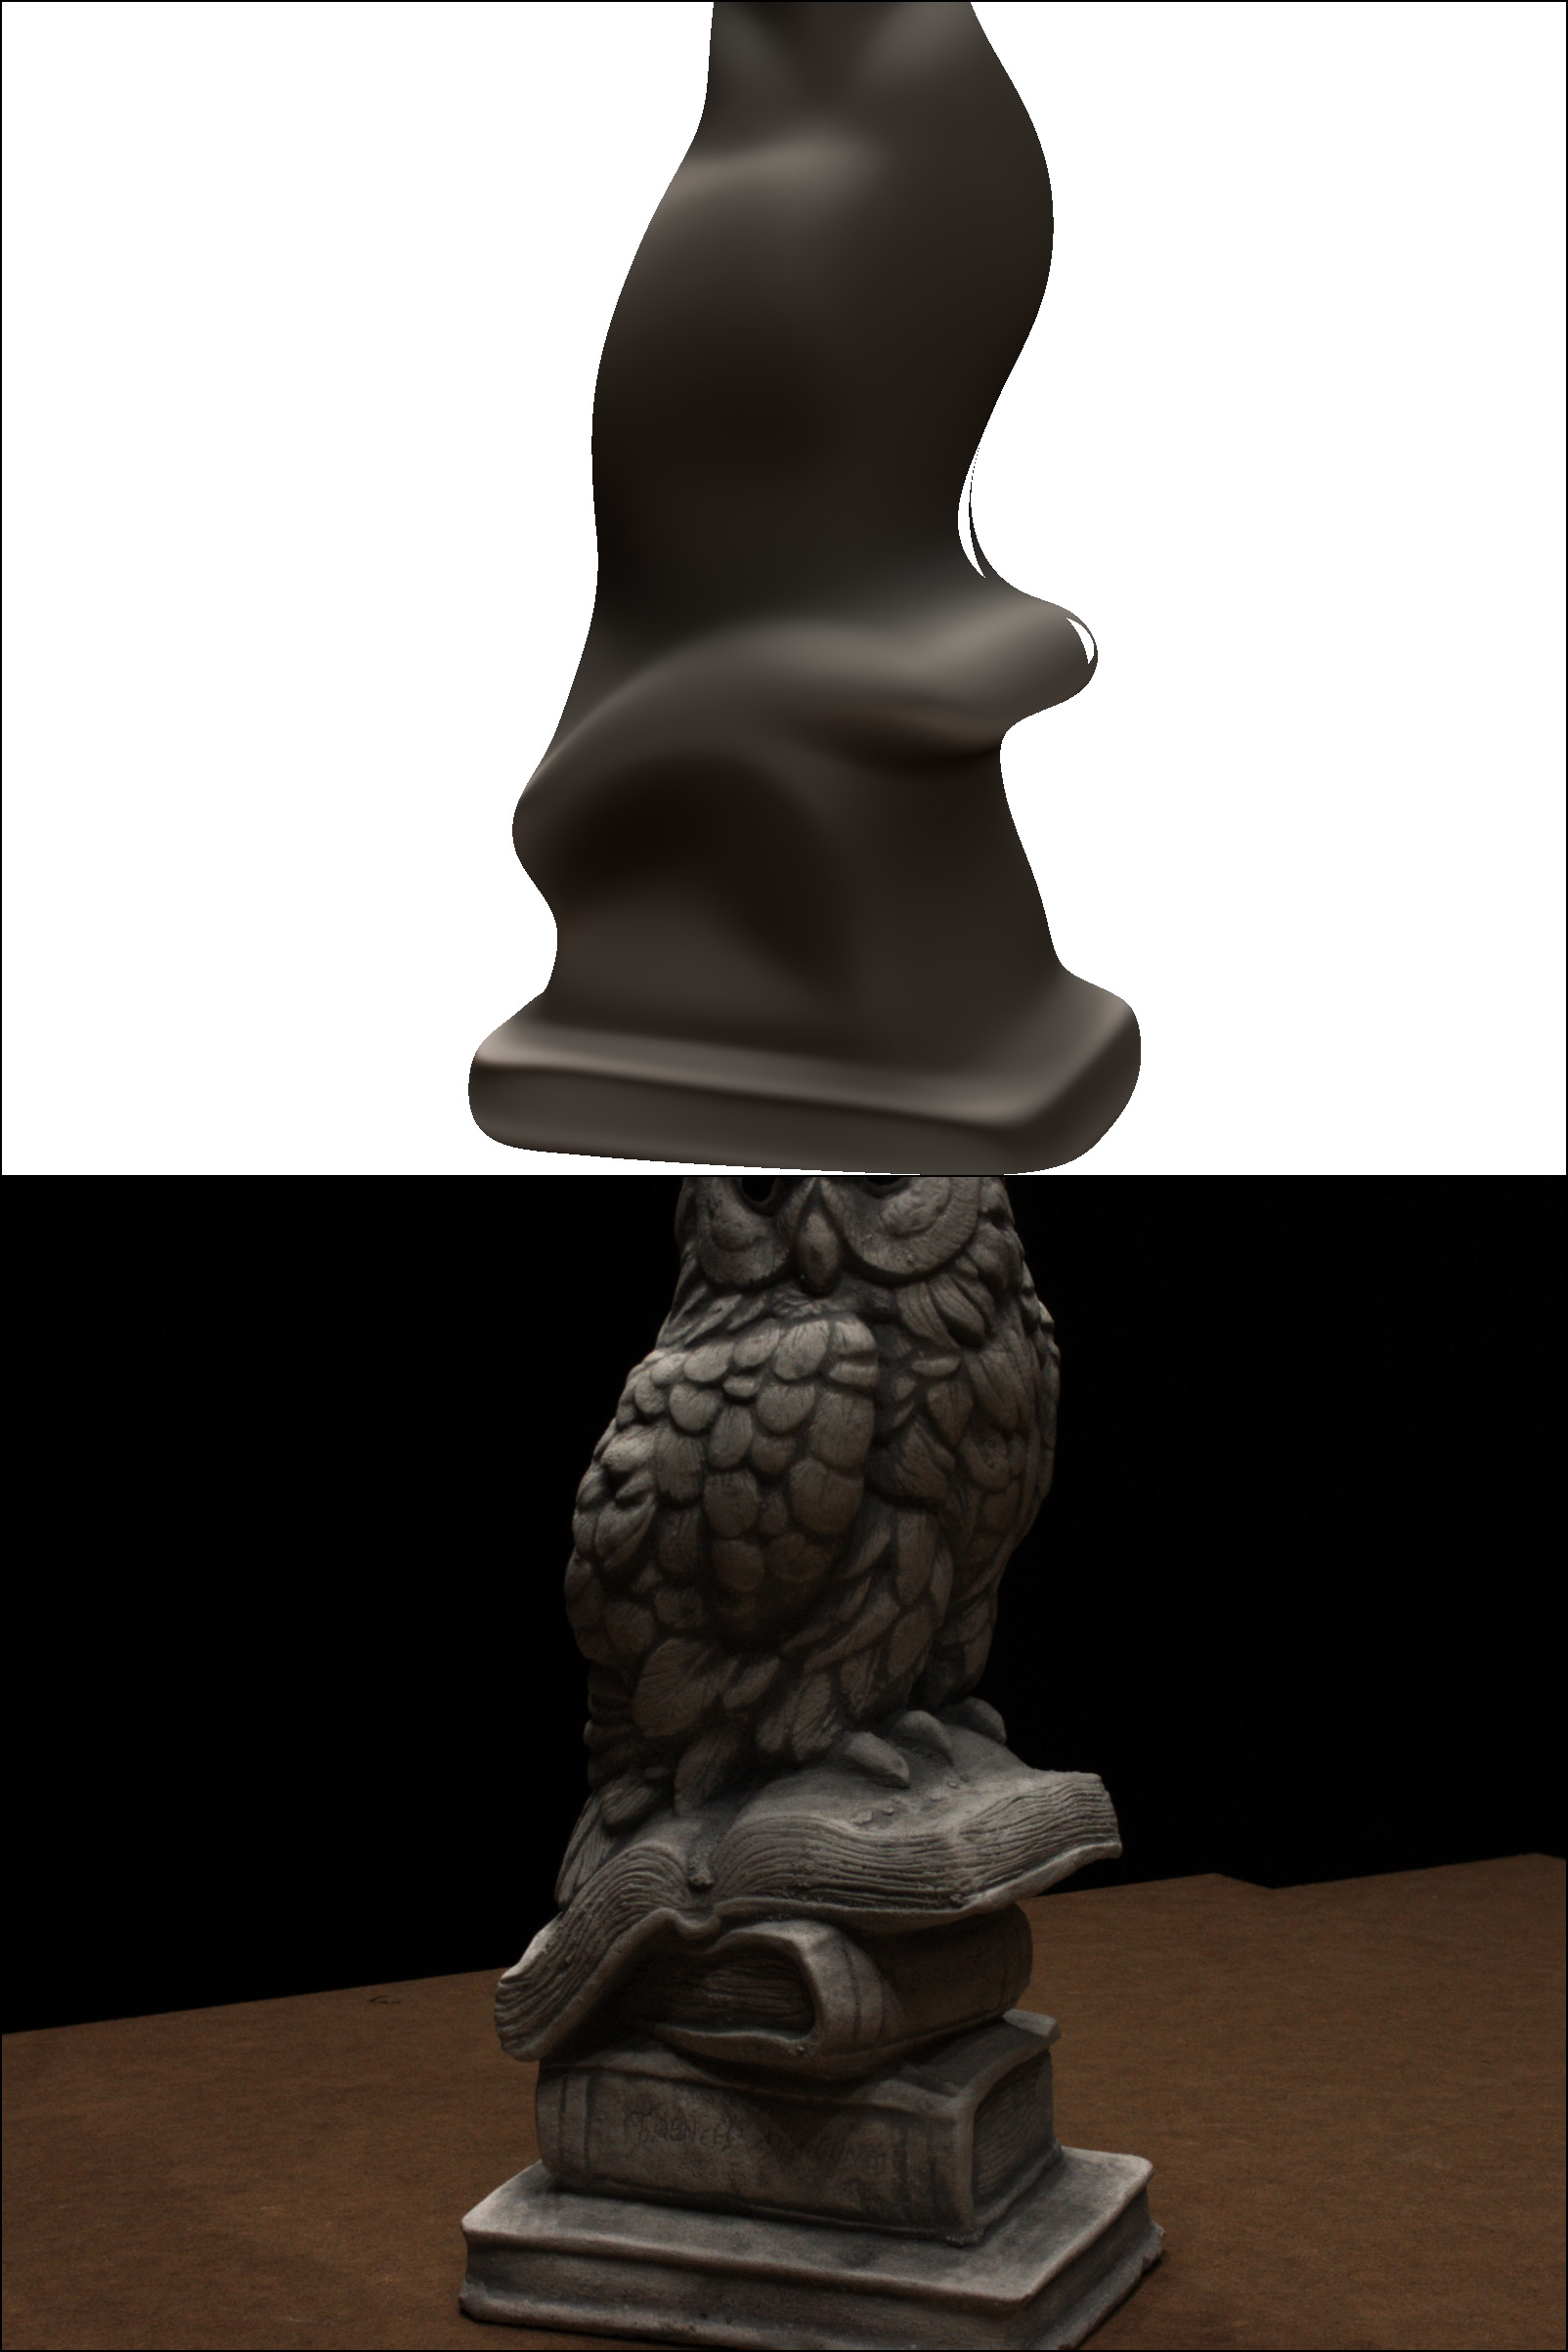
\includegraphics[width=1.5cm]{images/chapter5_img/RenderedImages-DepthMaps-EpochWise-Evals/PositionalEncoding/122/rendering_100.jpg} & 
     &
     & 
     & 
    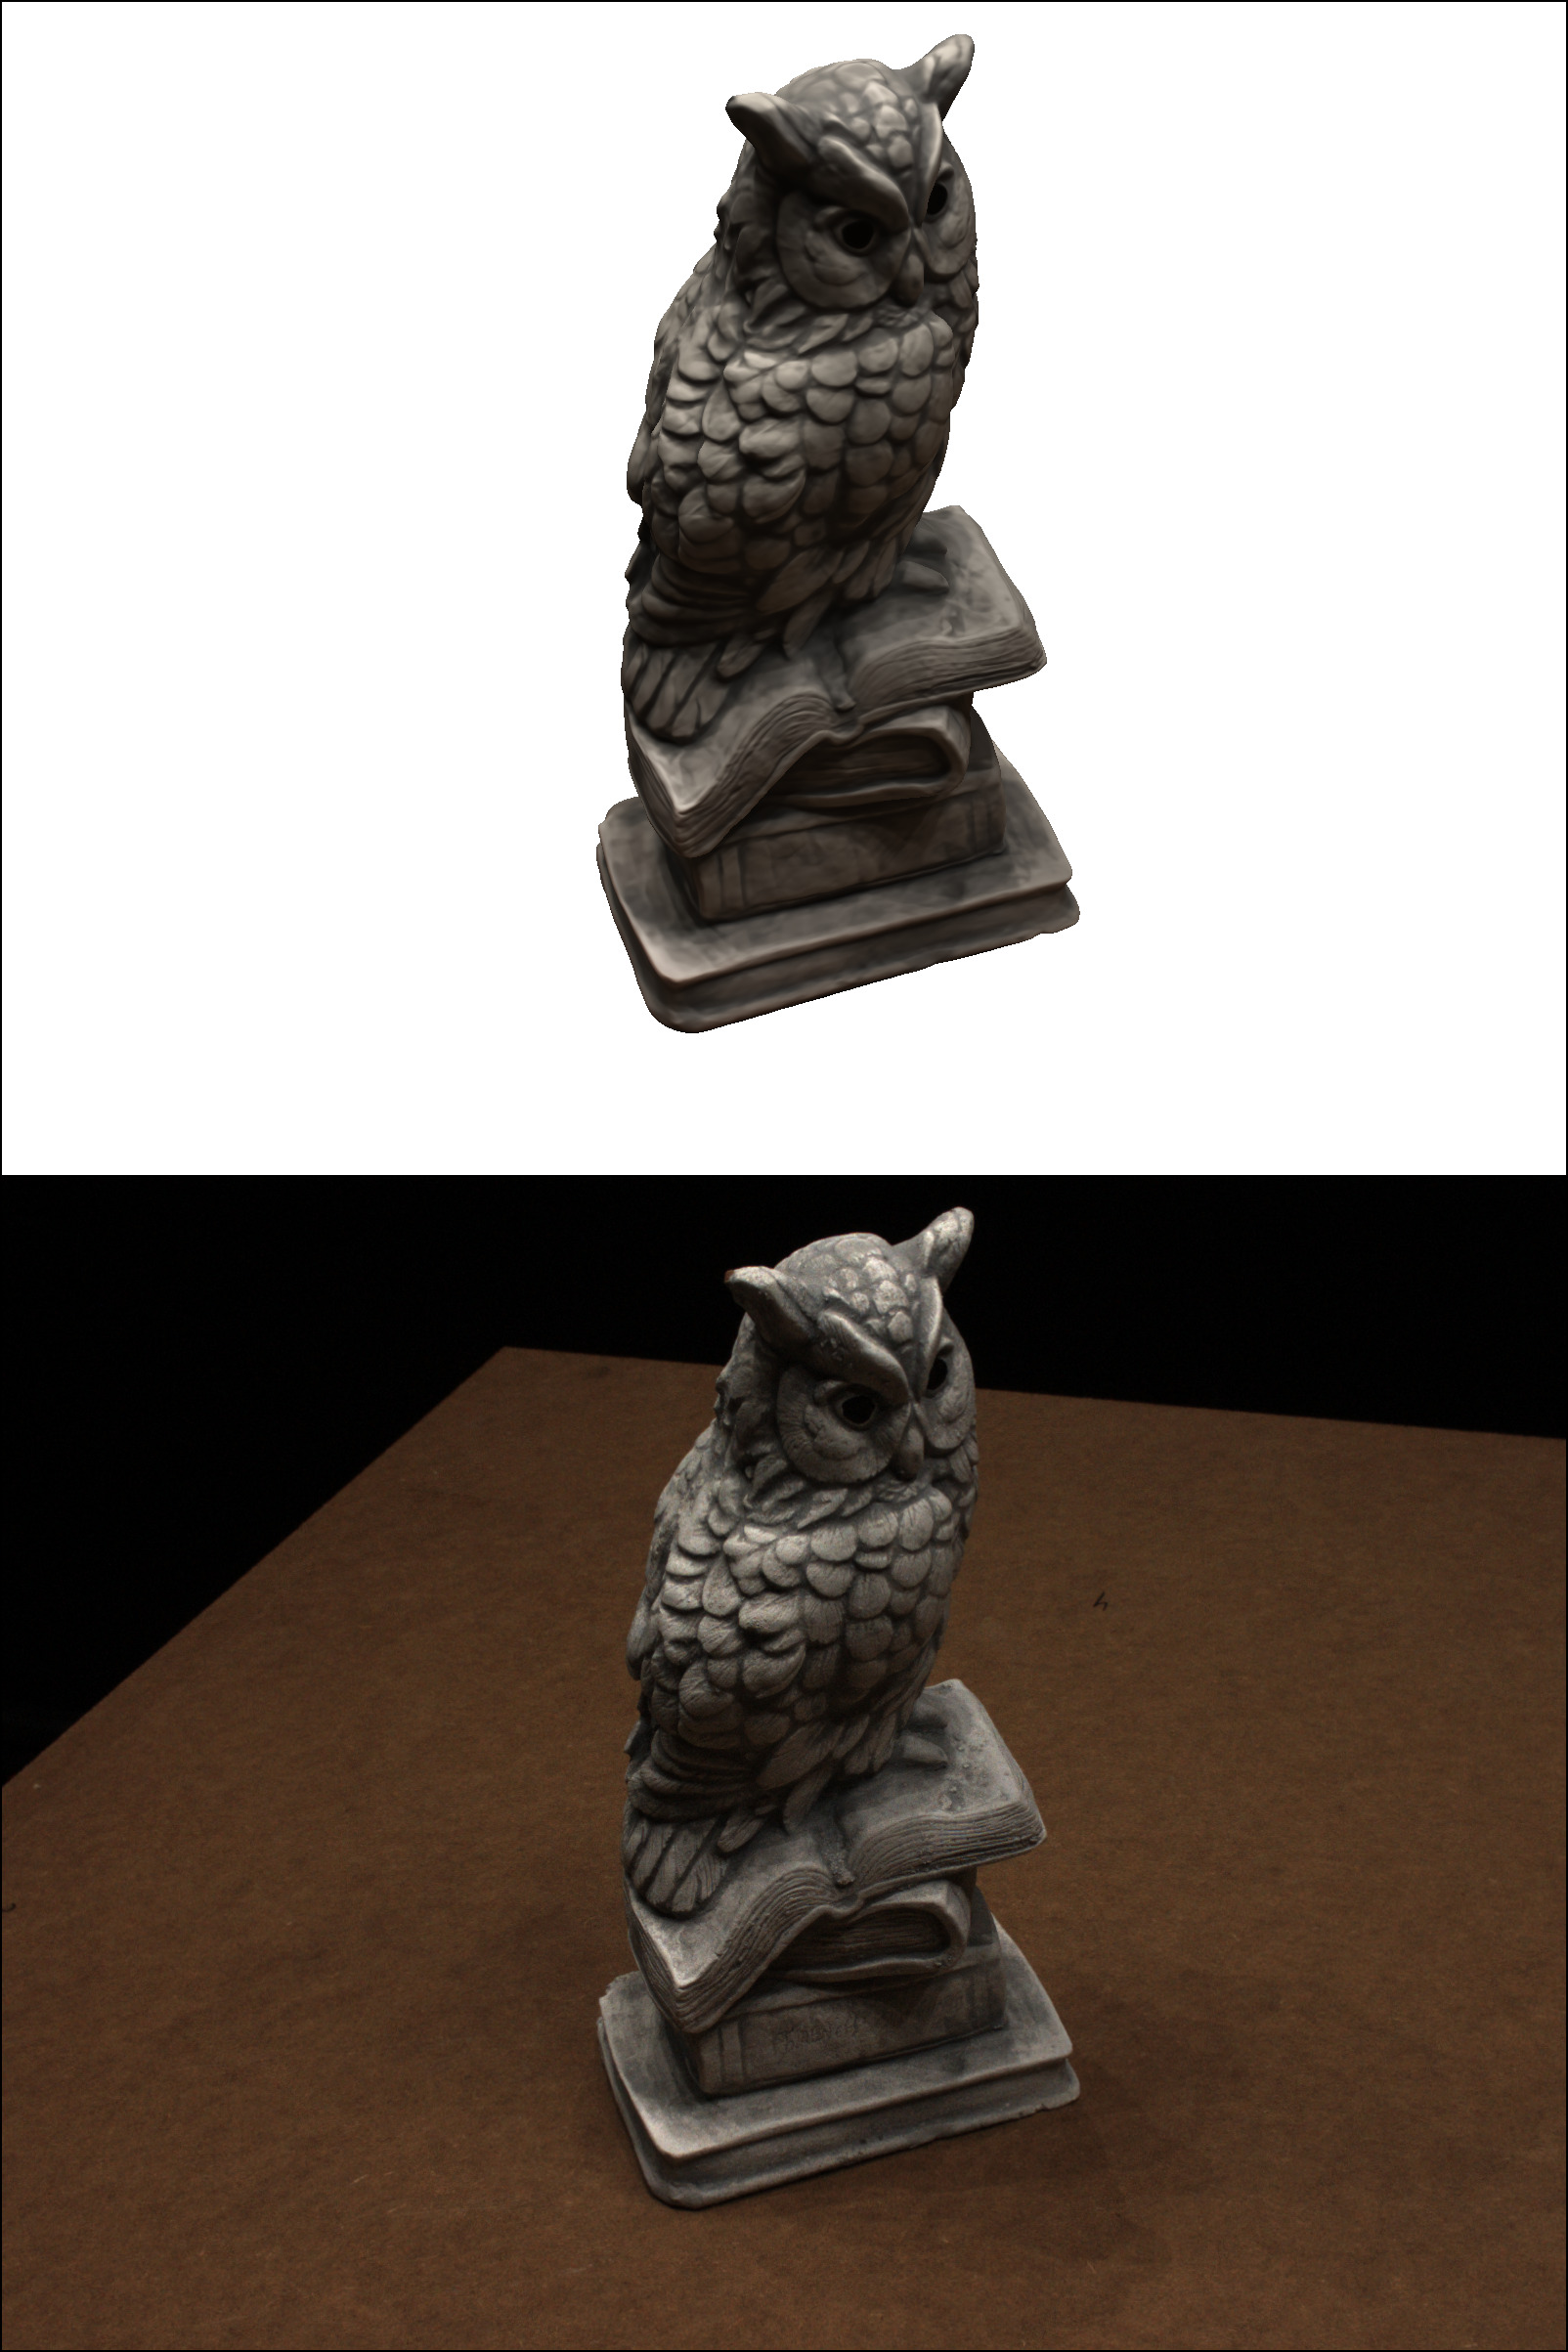
\includegraphics[width=1.5cm]{images/chapter5_img/RenderedImages-DepthMaps-EpochWise-Evals/PositionalEncoding/122/rendering_2000.jpg} & 
    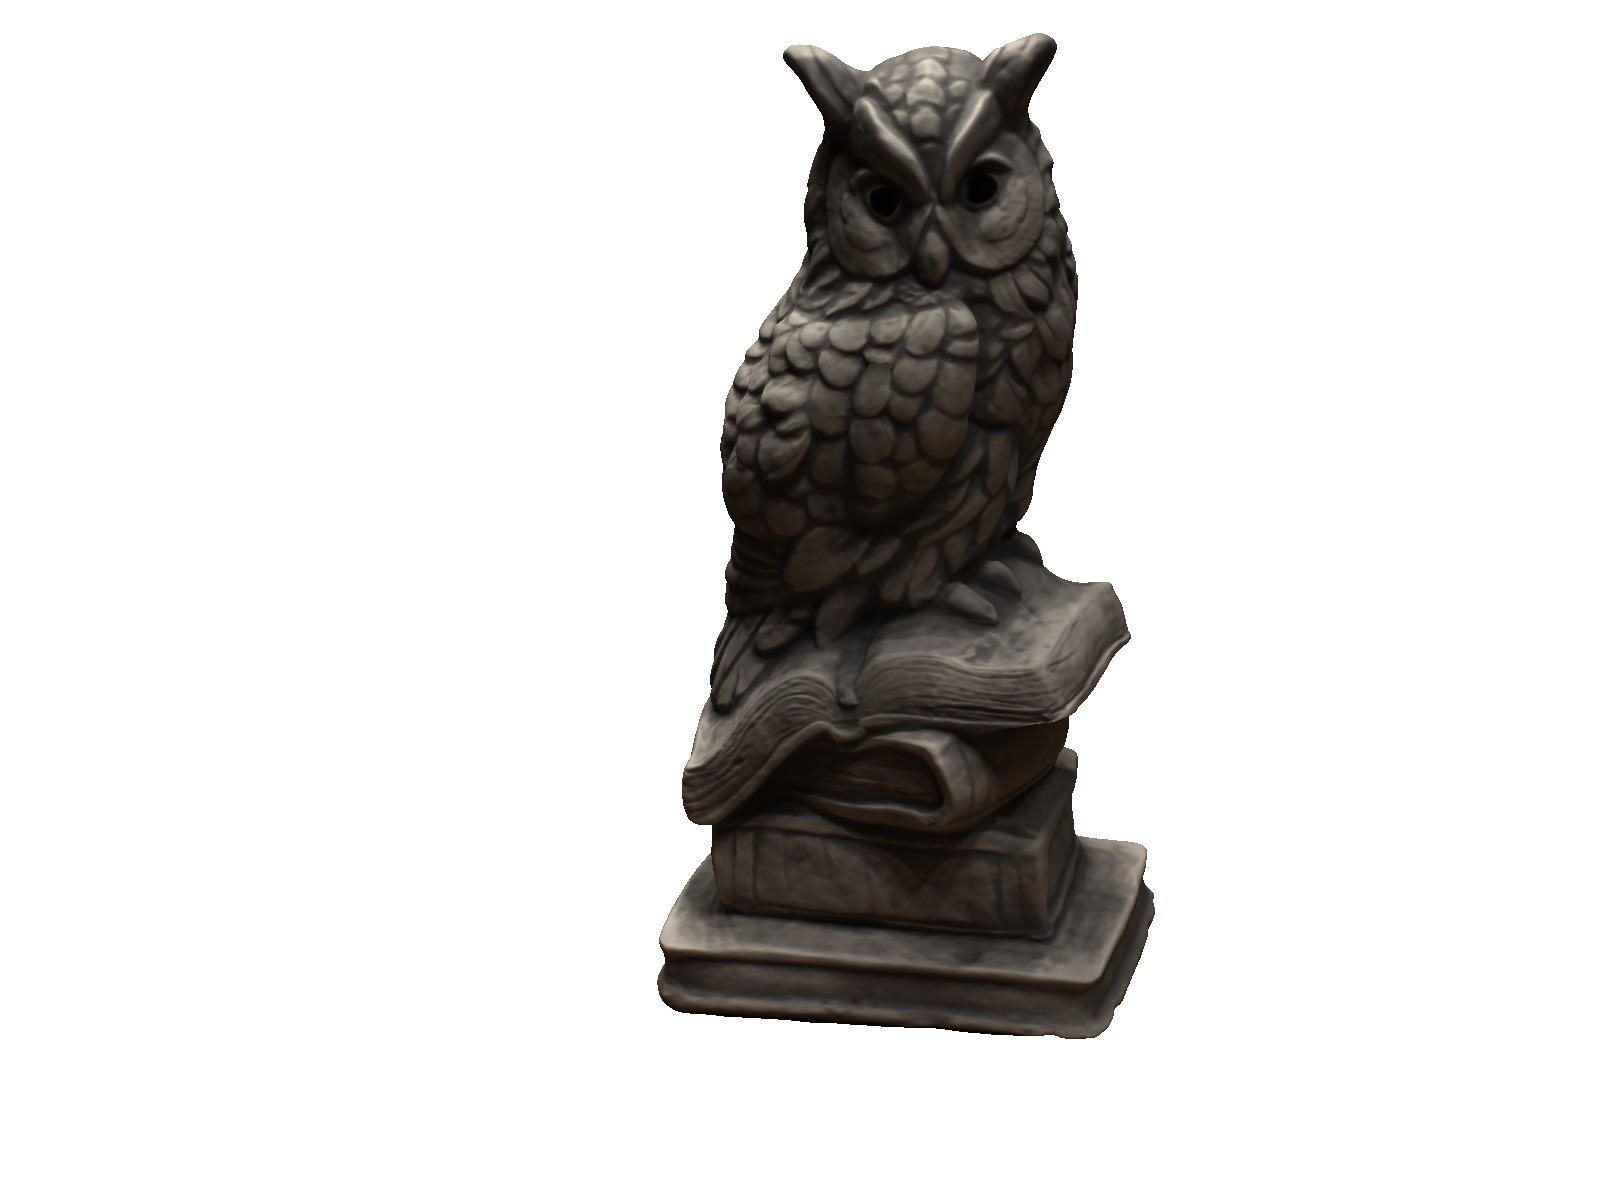
\includegraphics[width=1.5cm]{images/chapter5_img/RenderedImages-DepthMaps-EpochWise-Evals/PositionalEncoding/122/eval_055.jpg} \\
    \hline
    FourierNTK & 
    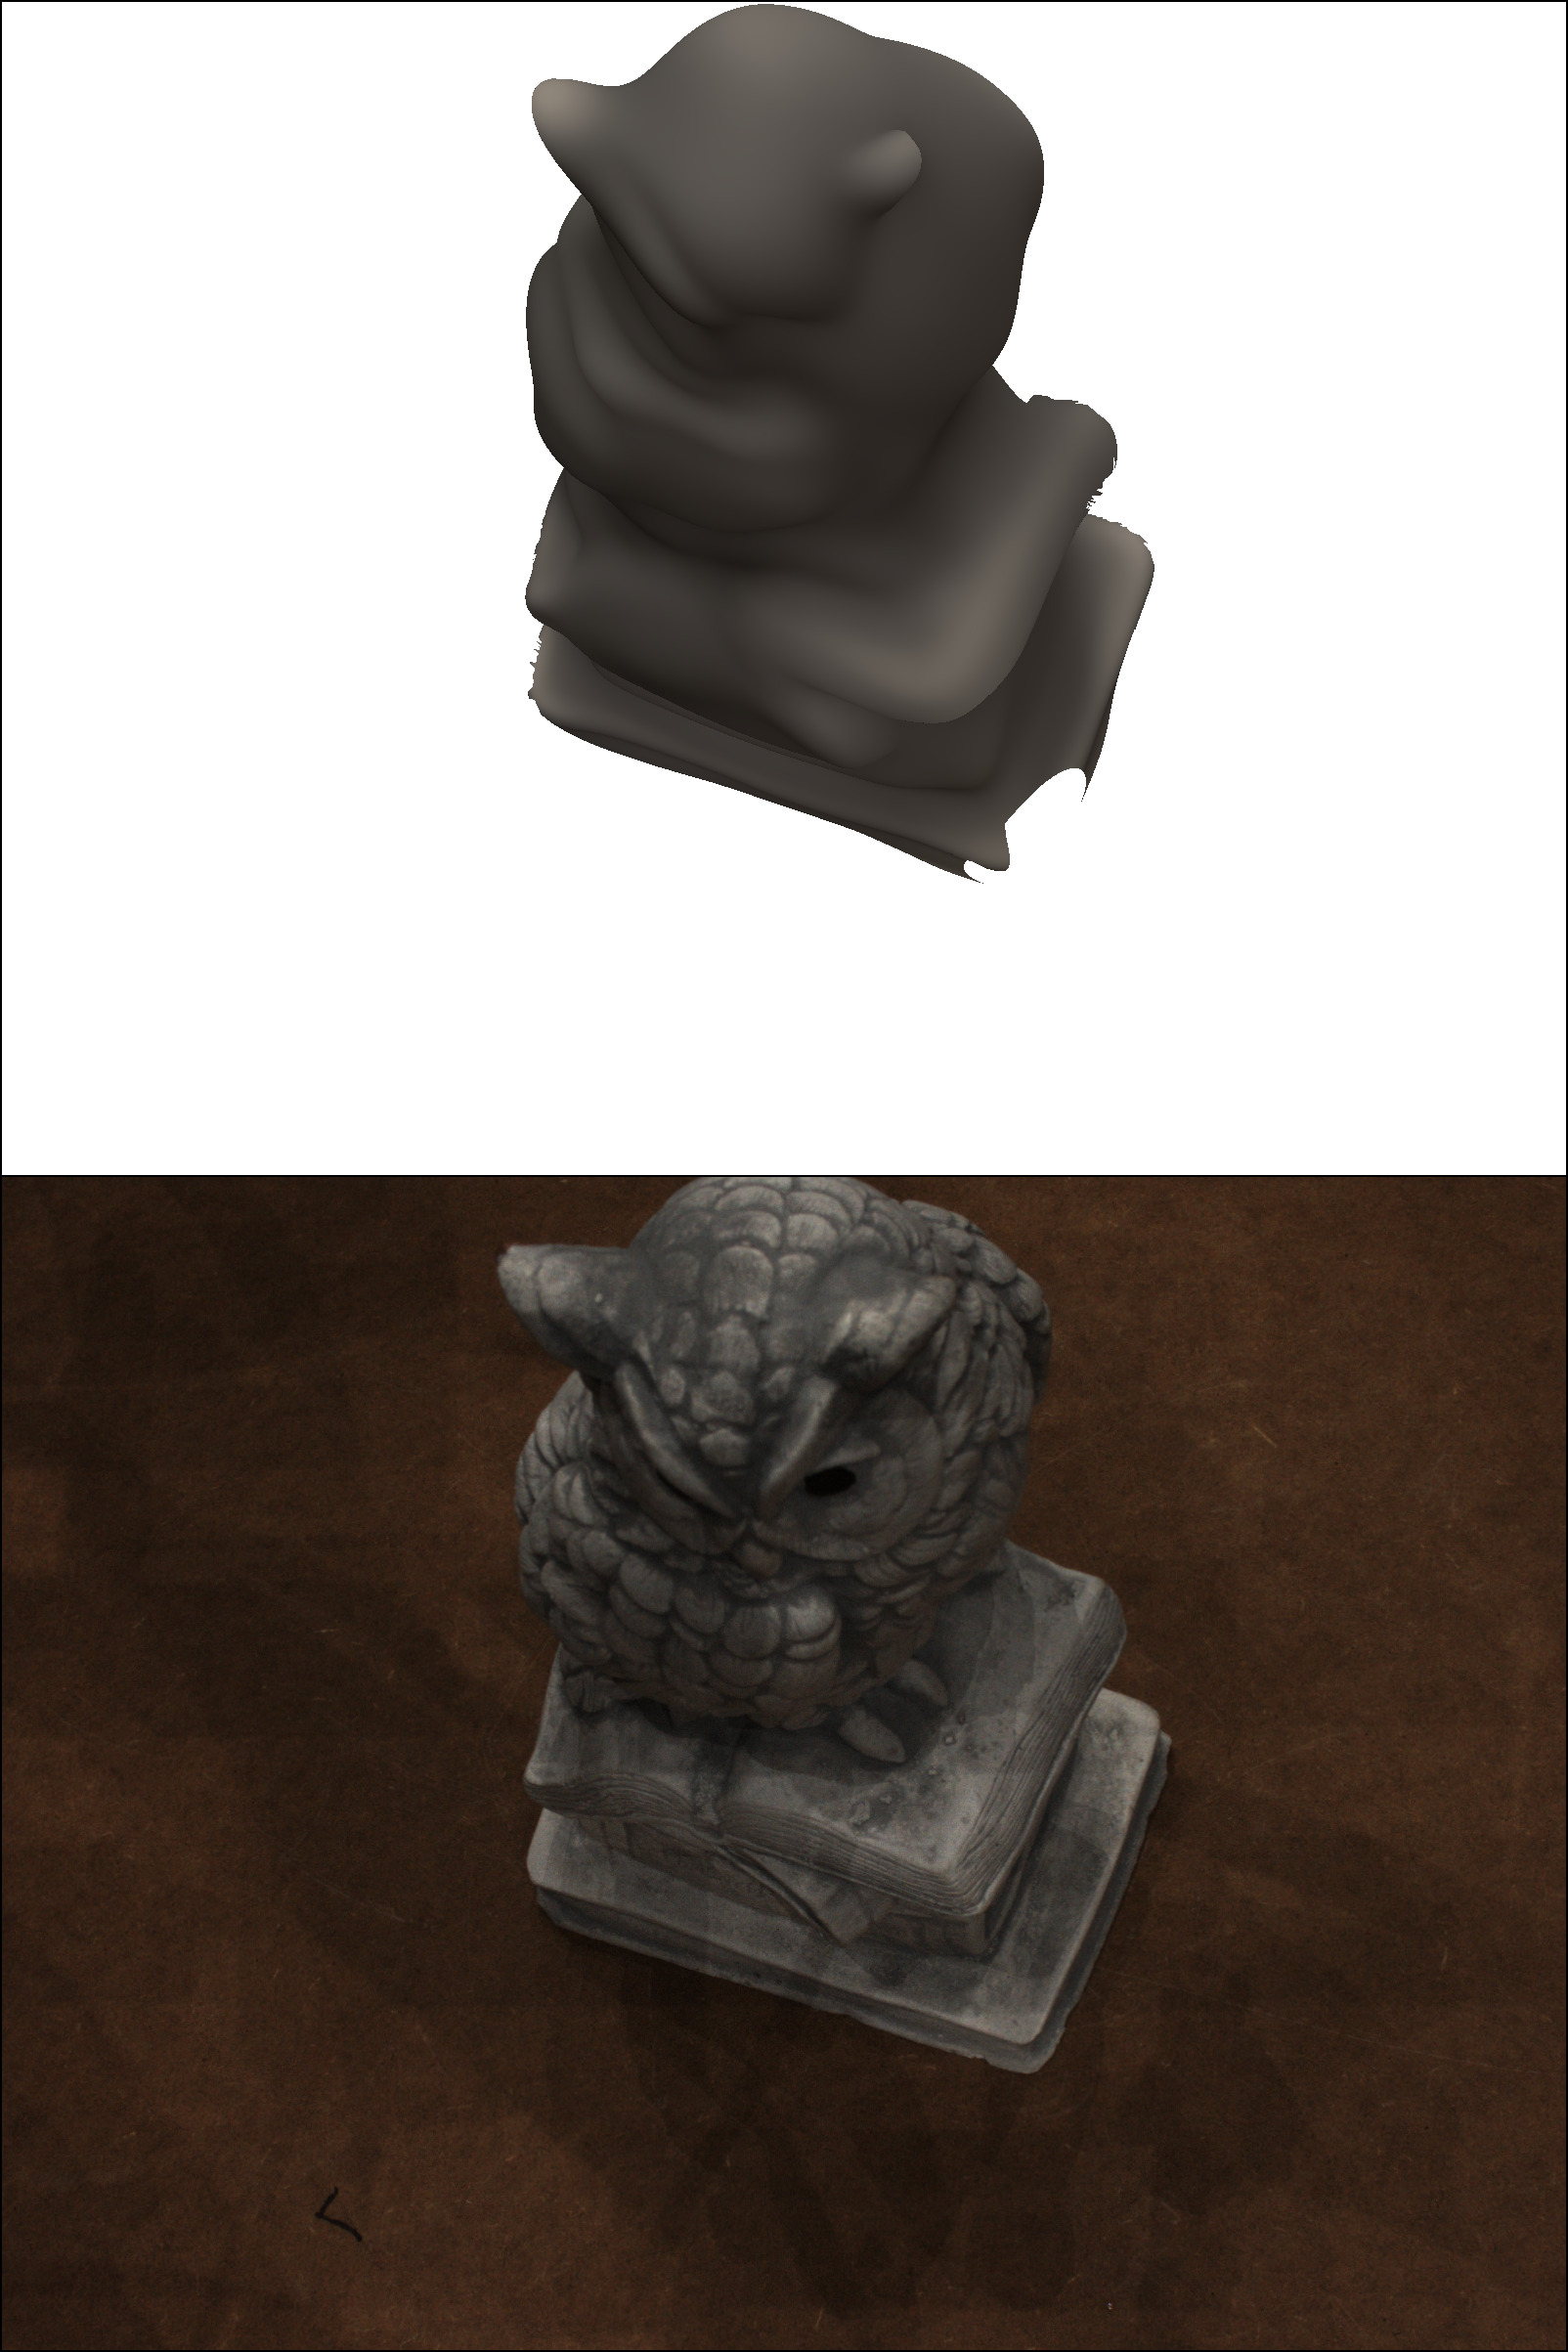
\includegraphics[width=1.5cm]{images/chapter5_img/RenderedImages-DepthMaps-EpochWise-Evals/FourierNTK/122/rendering_100.jpg} & 
    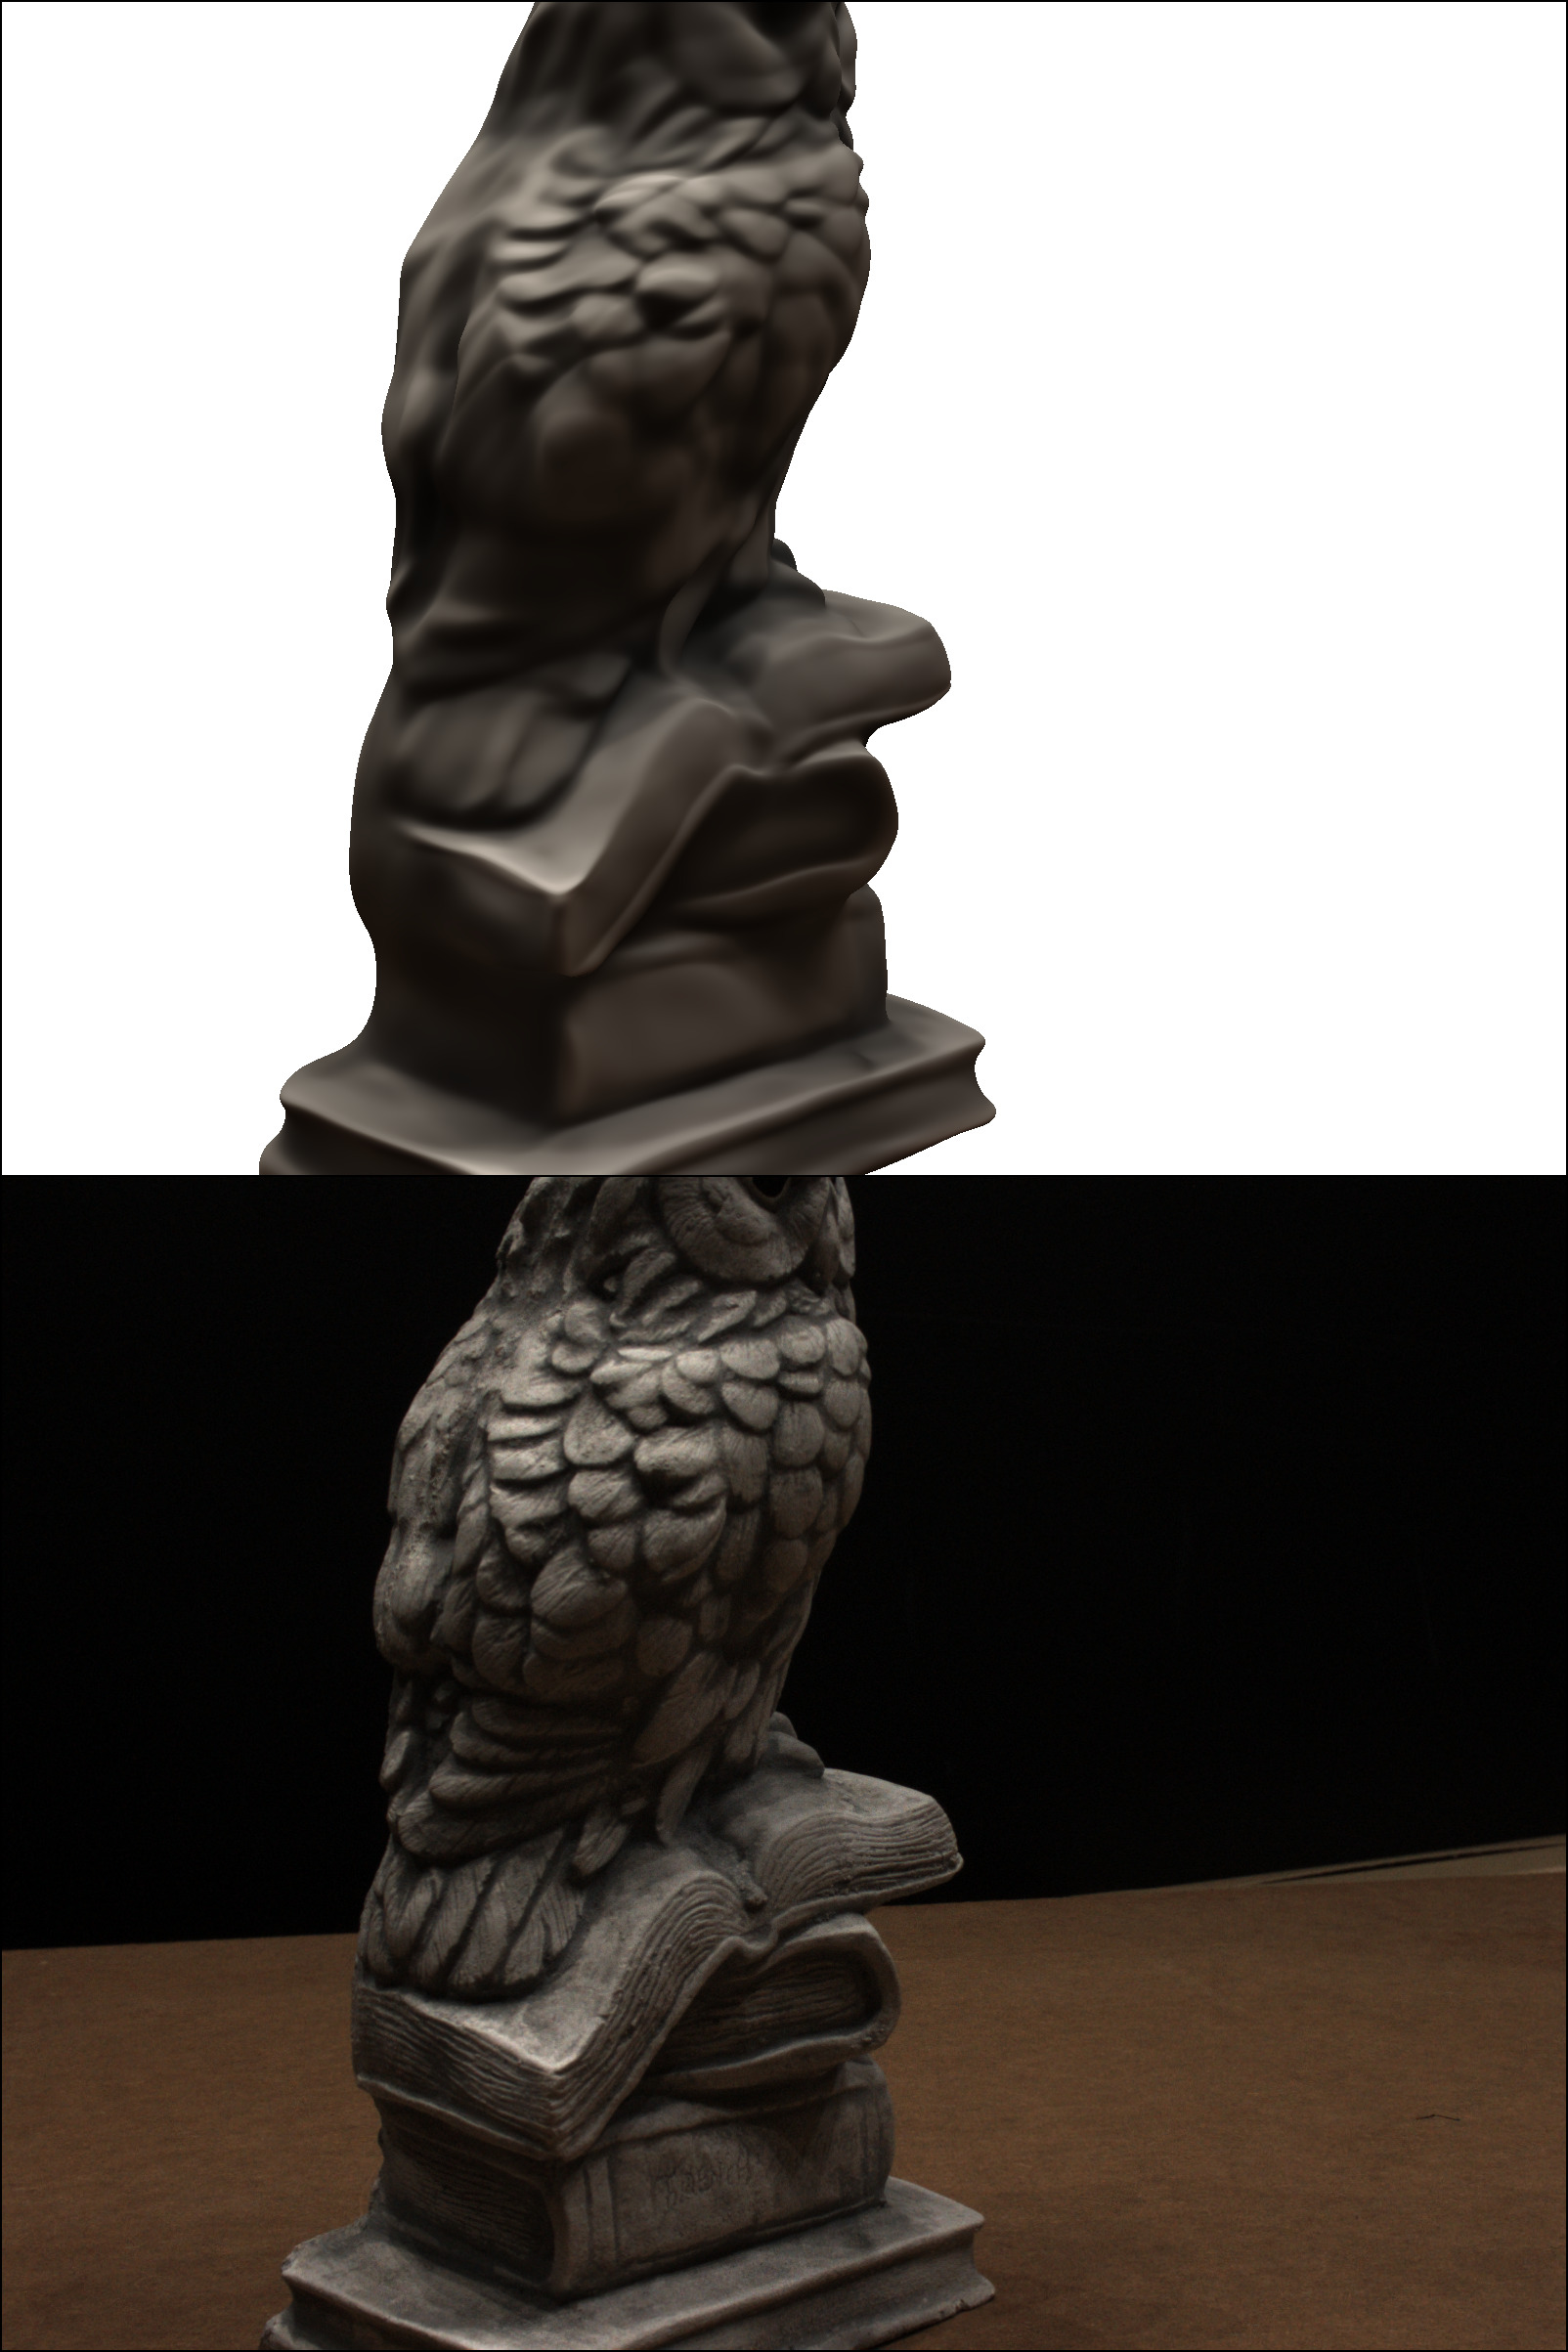
\includegraphics[width=1.5cm]{images/chapter5_img/RenderedImages-DepthMaps-EpochWise-Evals/FourierNTK/122/rendering_500.jpg} & 
    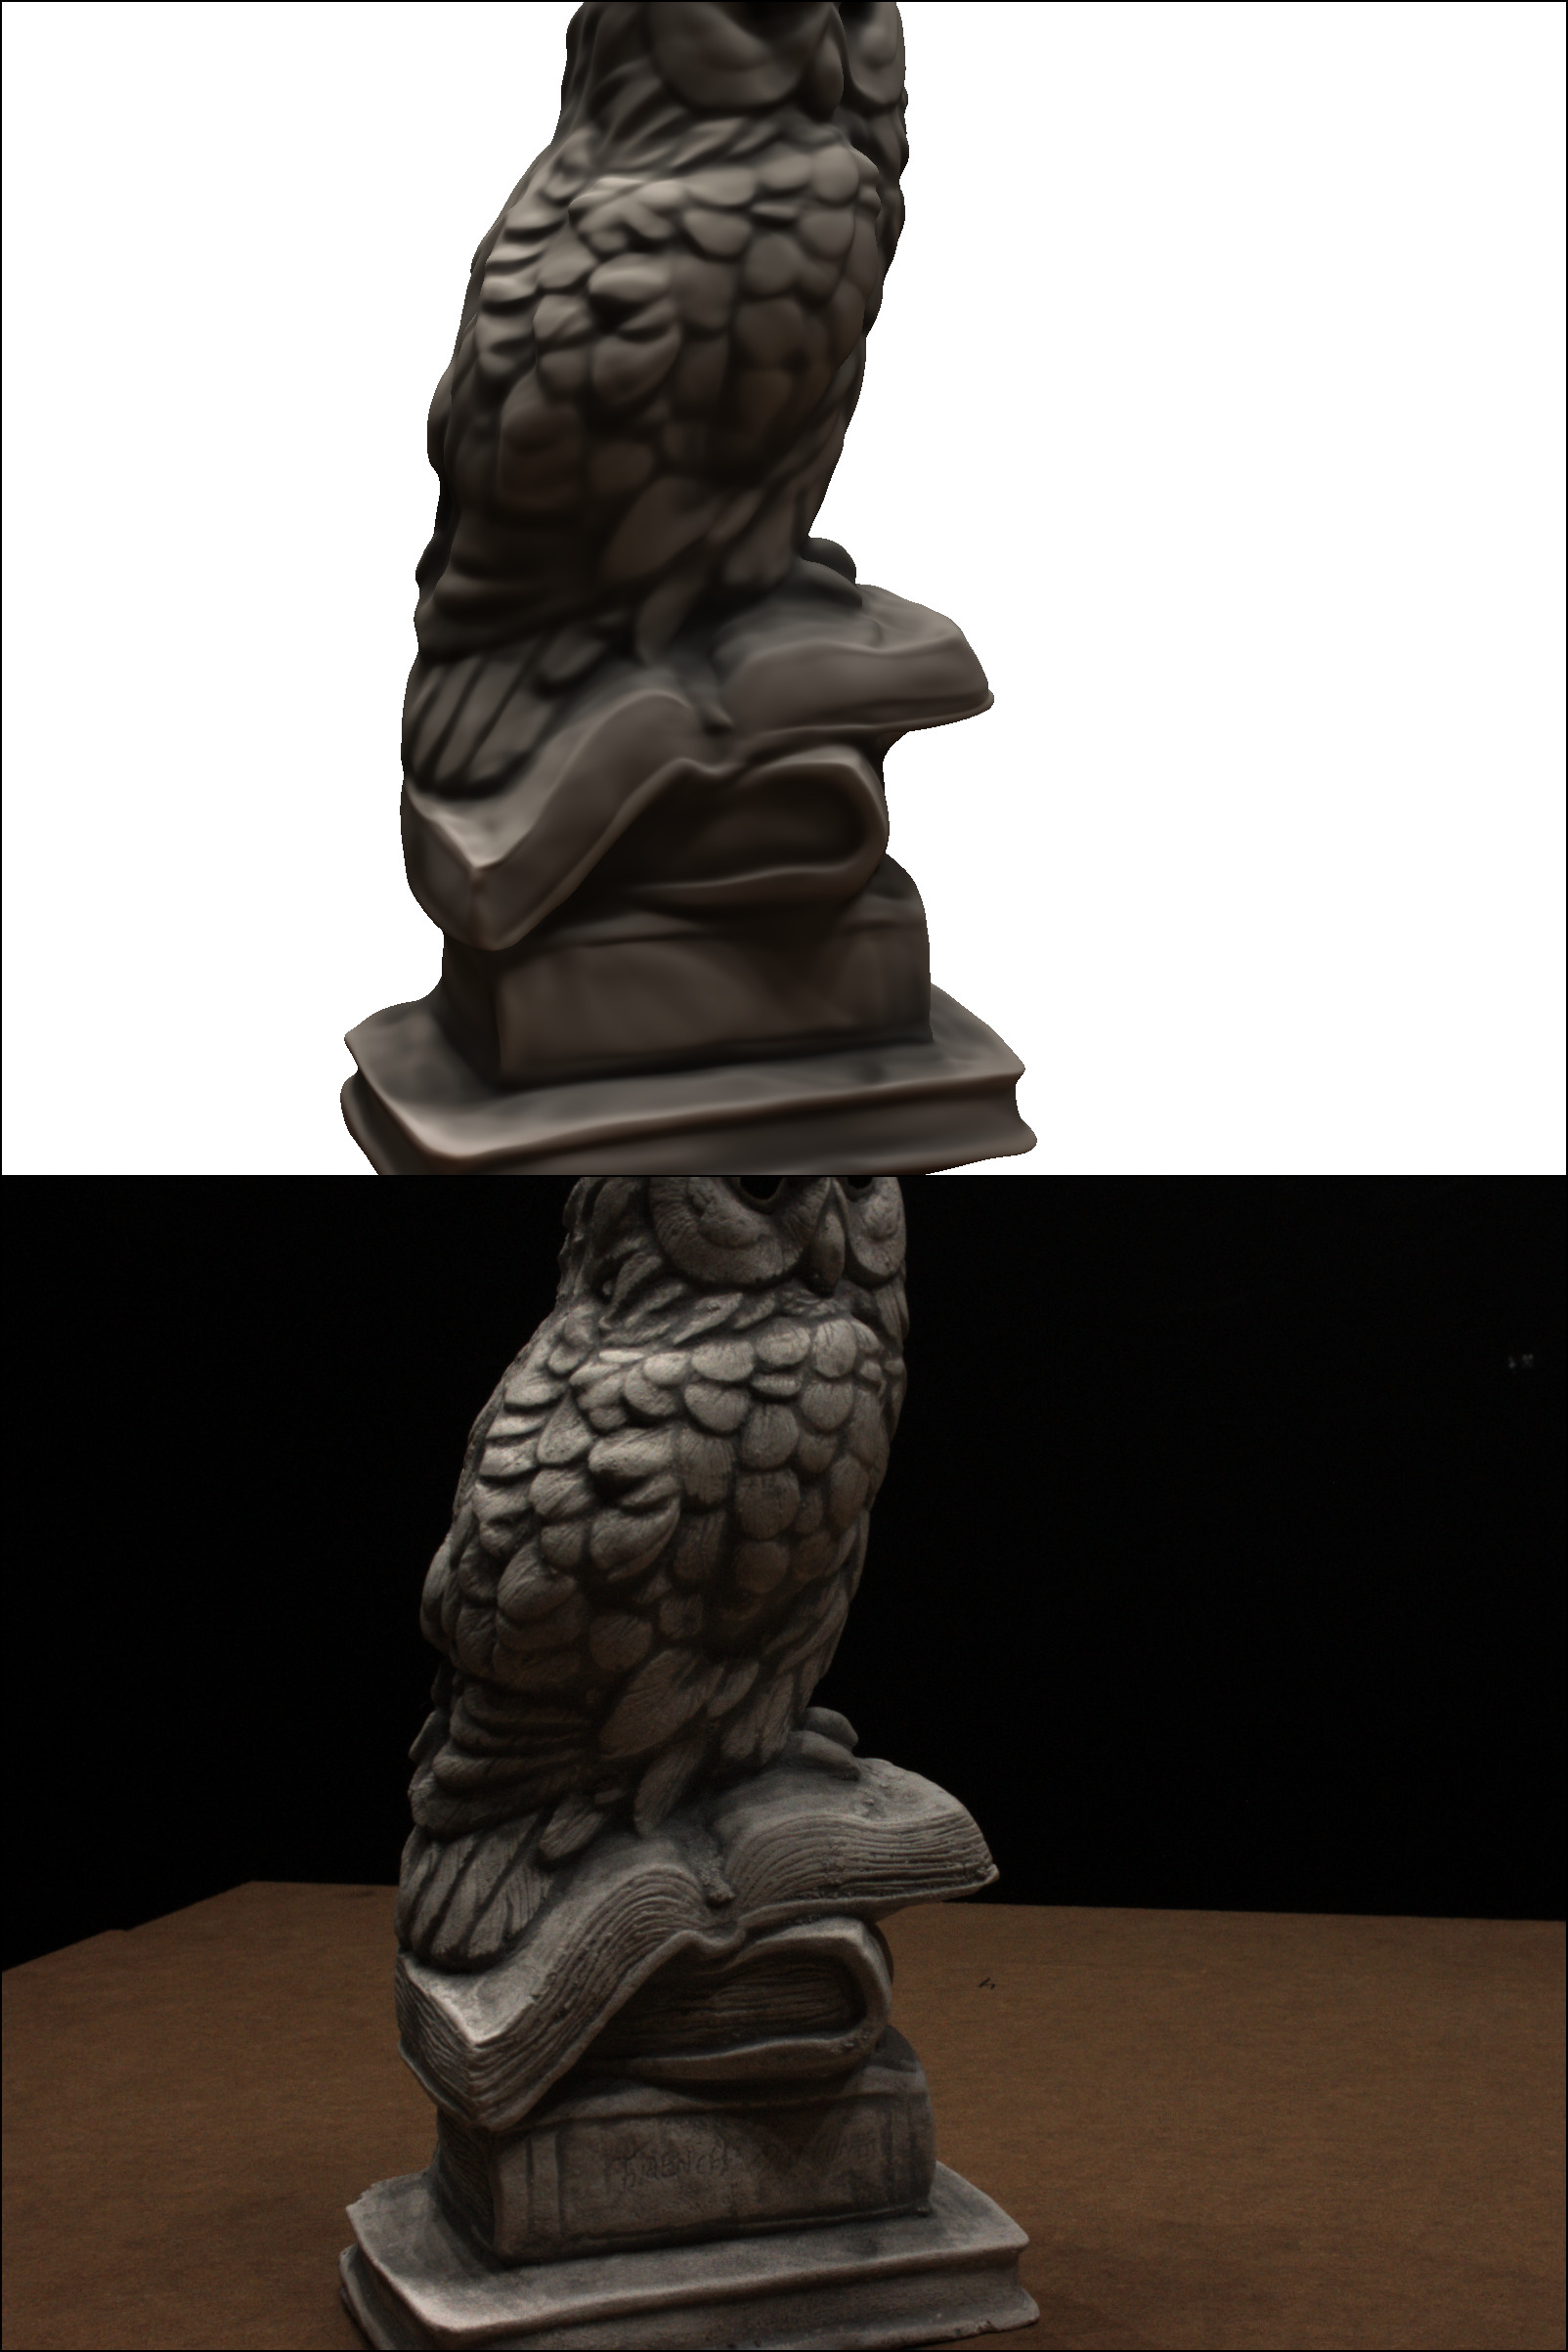
\includegraphics[width=1.5cm]{images/chapter5_img/RenderedImages-DepthMaps-EpochWise-Evals/FourierNTK/122/rendering_1000.jpg} & 
    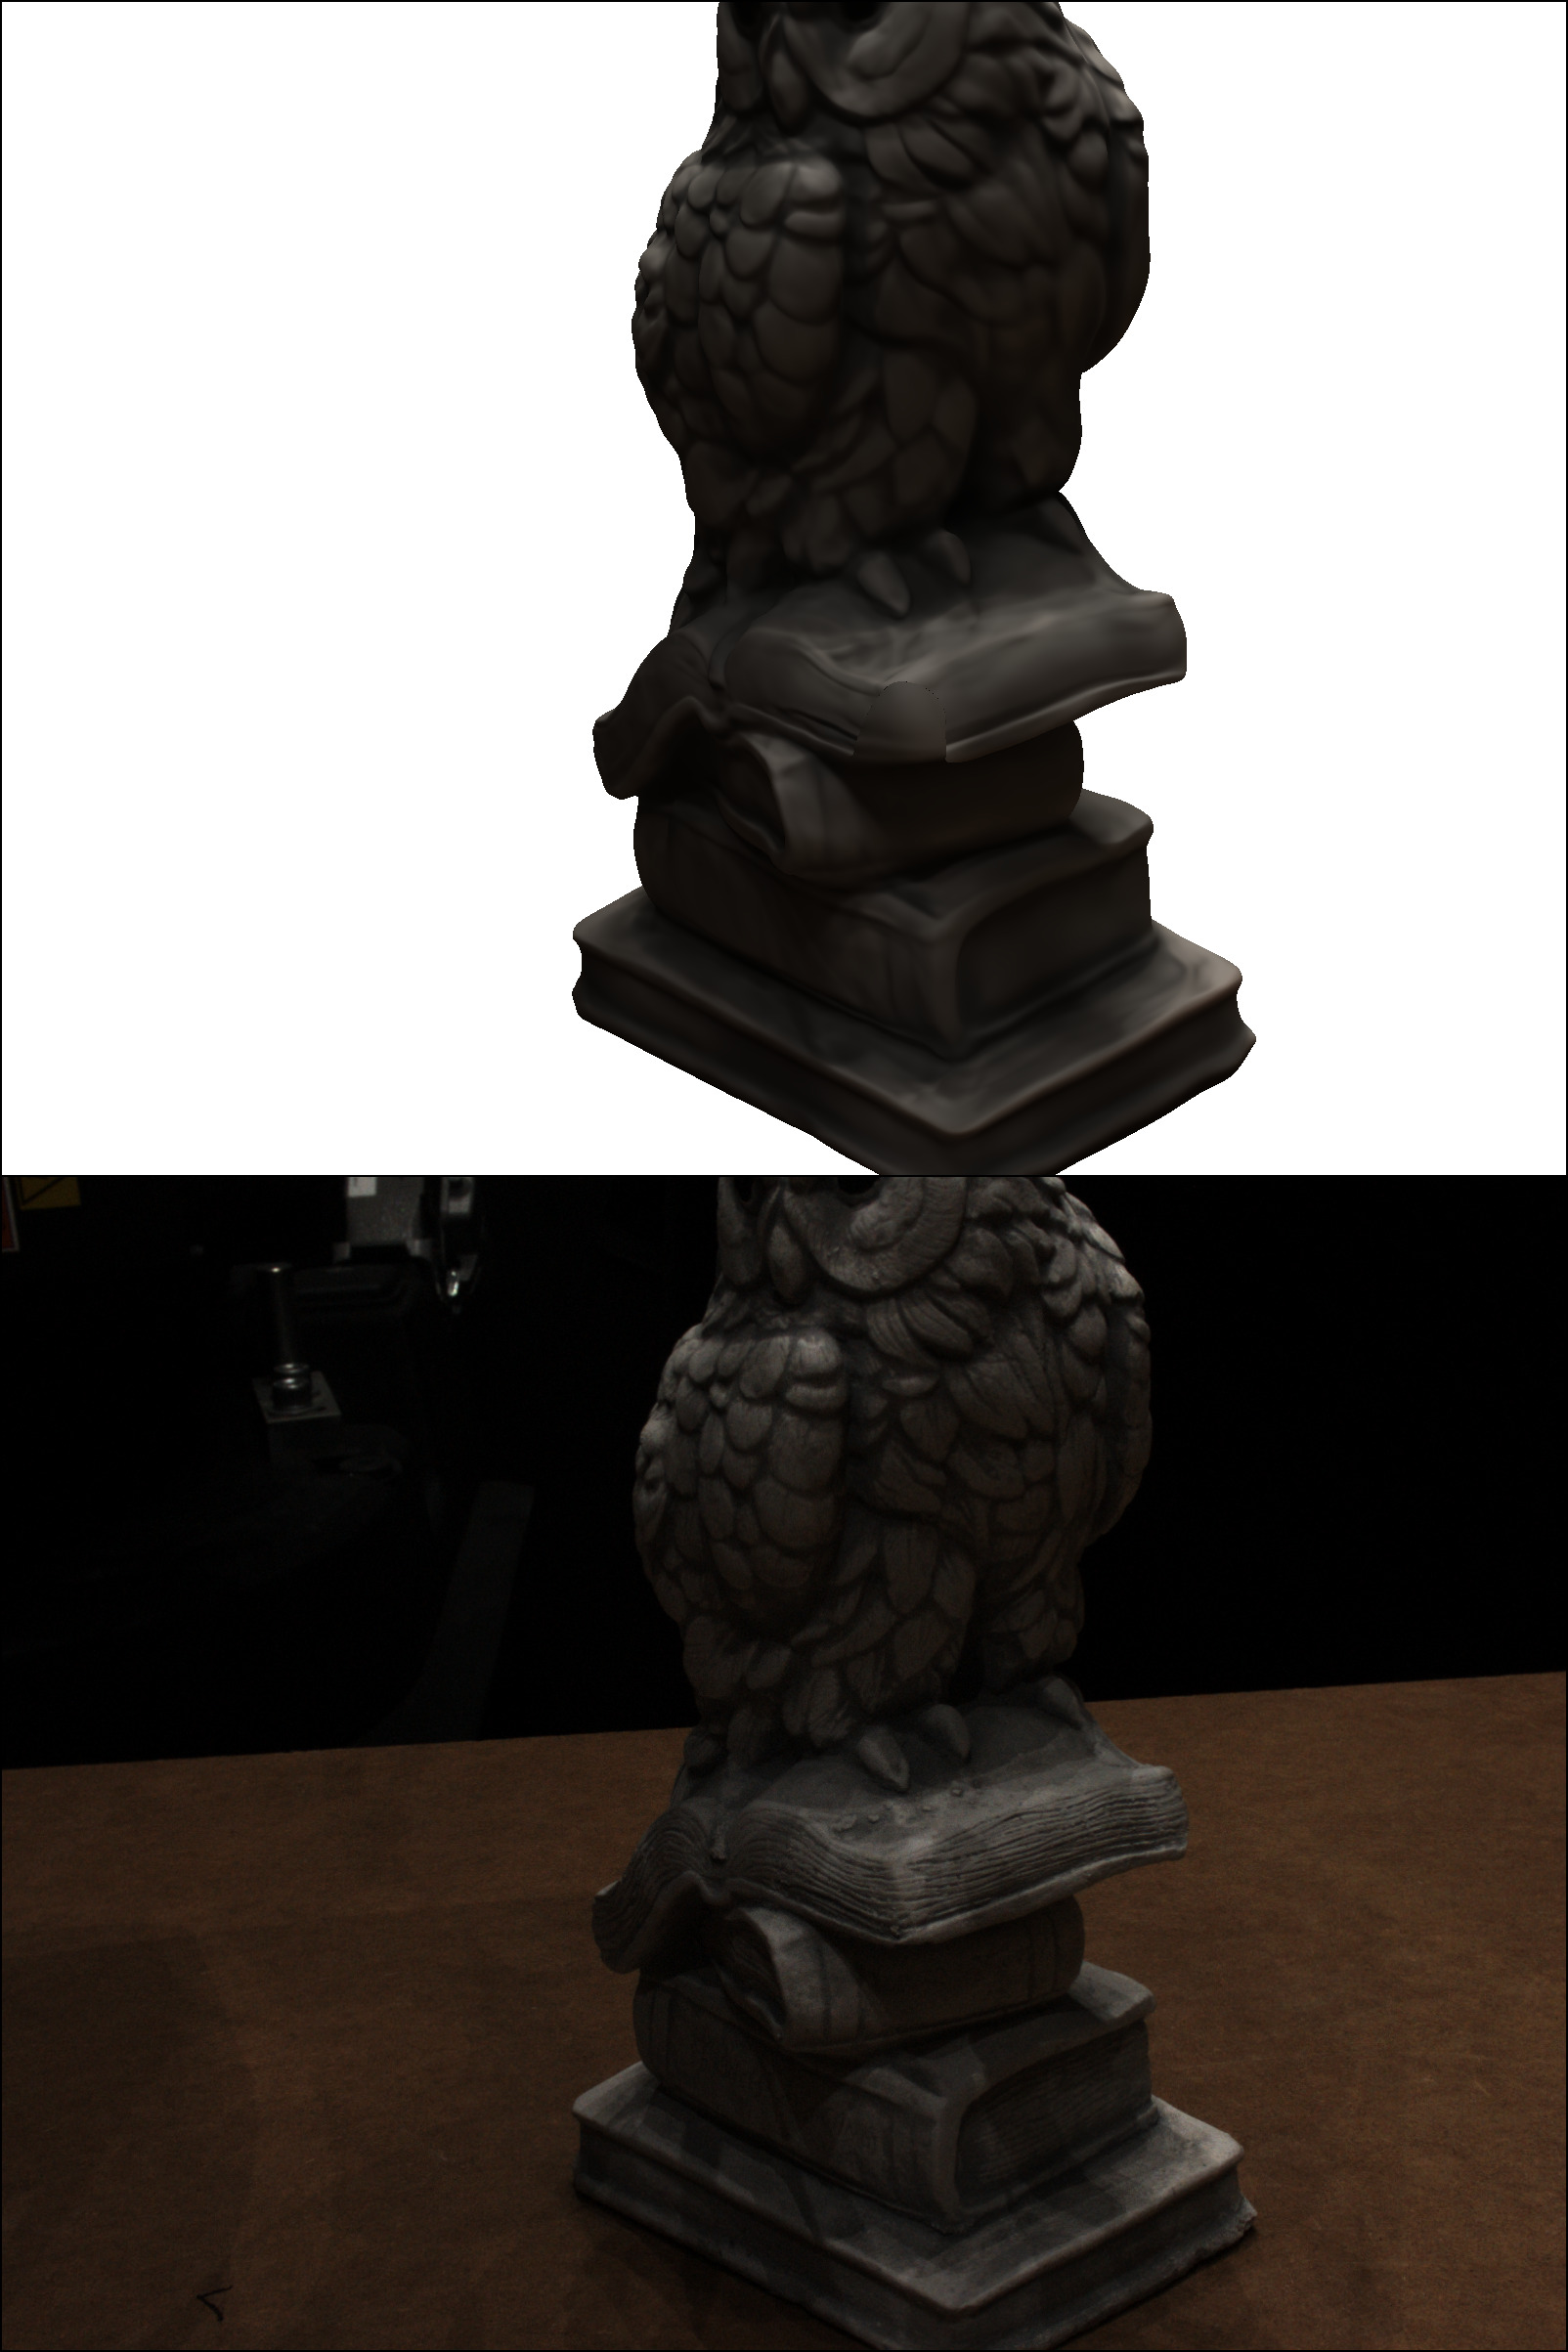
\includegraphics[width=1.5cm]{images/chapter5_img/RenderedImages-DepthMaps-EpochWise-Evals/FourierNTK/122/rendering_2000.jpg} & 
    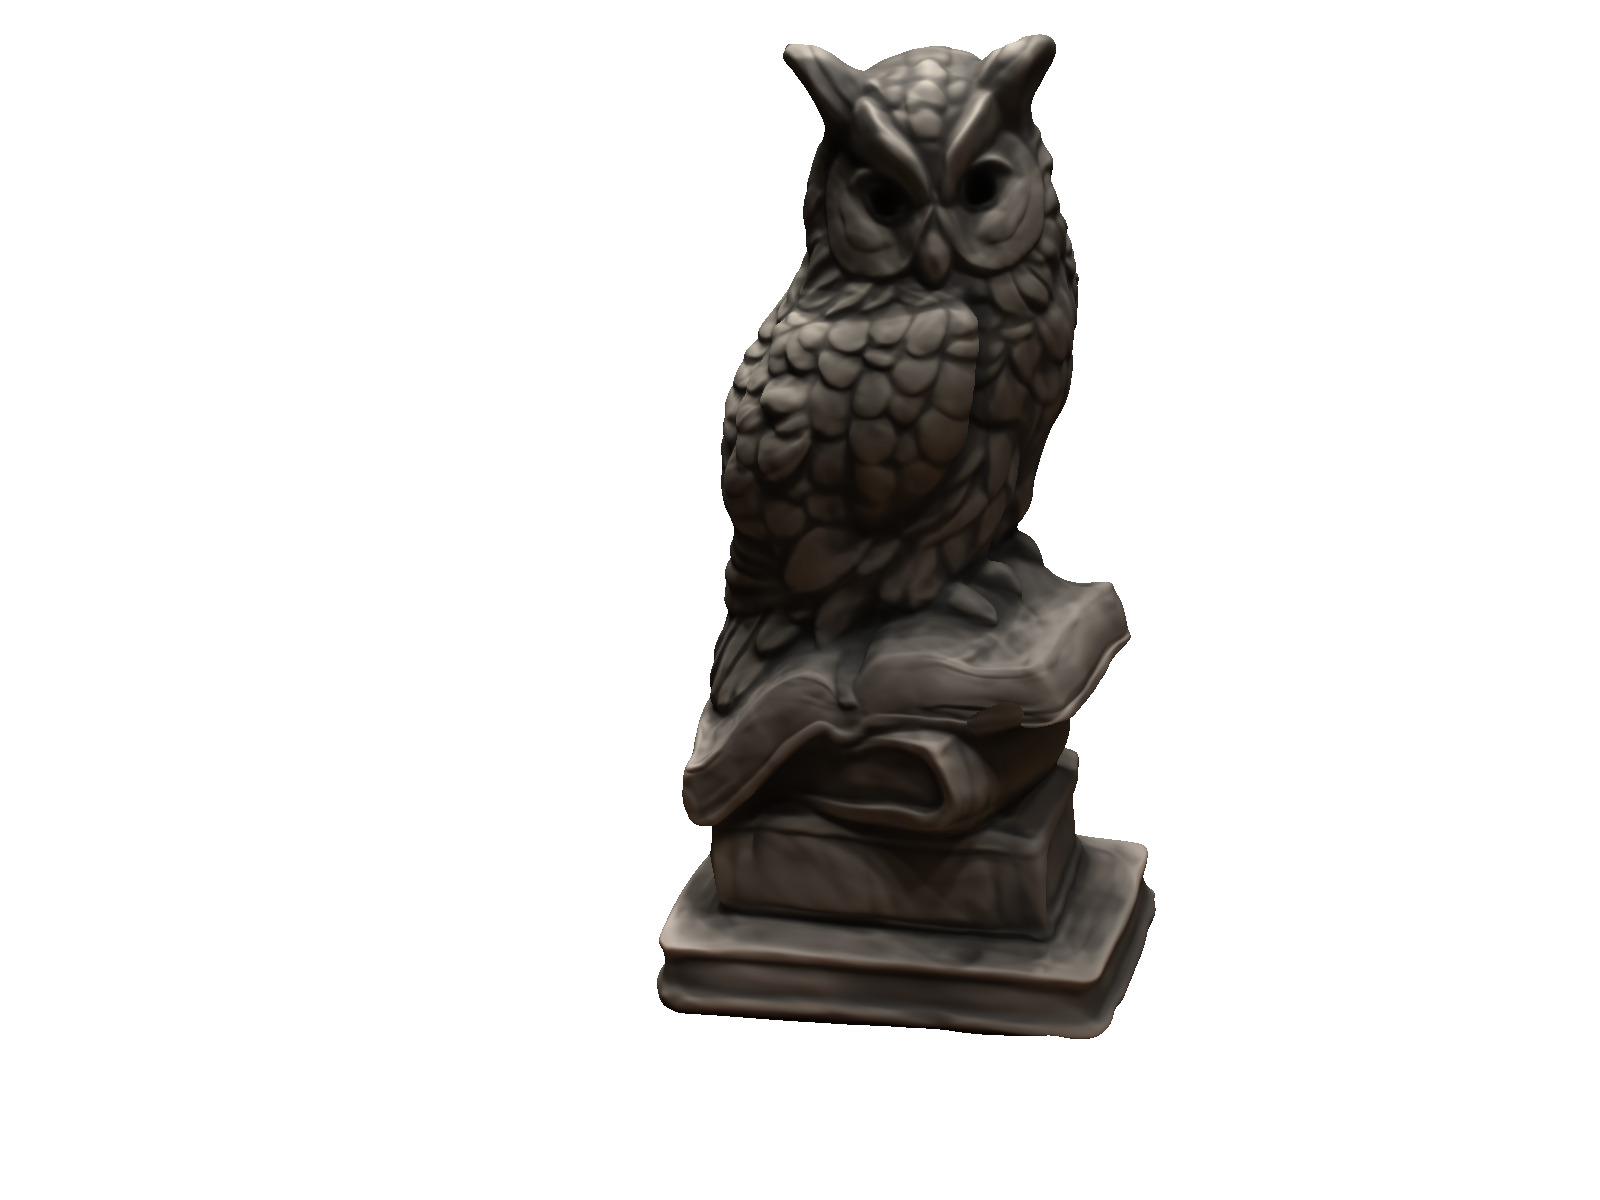
\includegraphics[width=1.5cm]{images/chapter5_img/RenderedImages-DepthMaps-EpochWise-Evals/FourierNTK/122/eval_055.jpg} \\
    \hline
    MR-HashGrid3D & 
    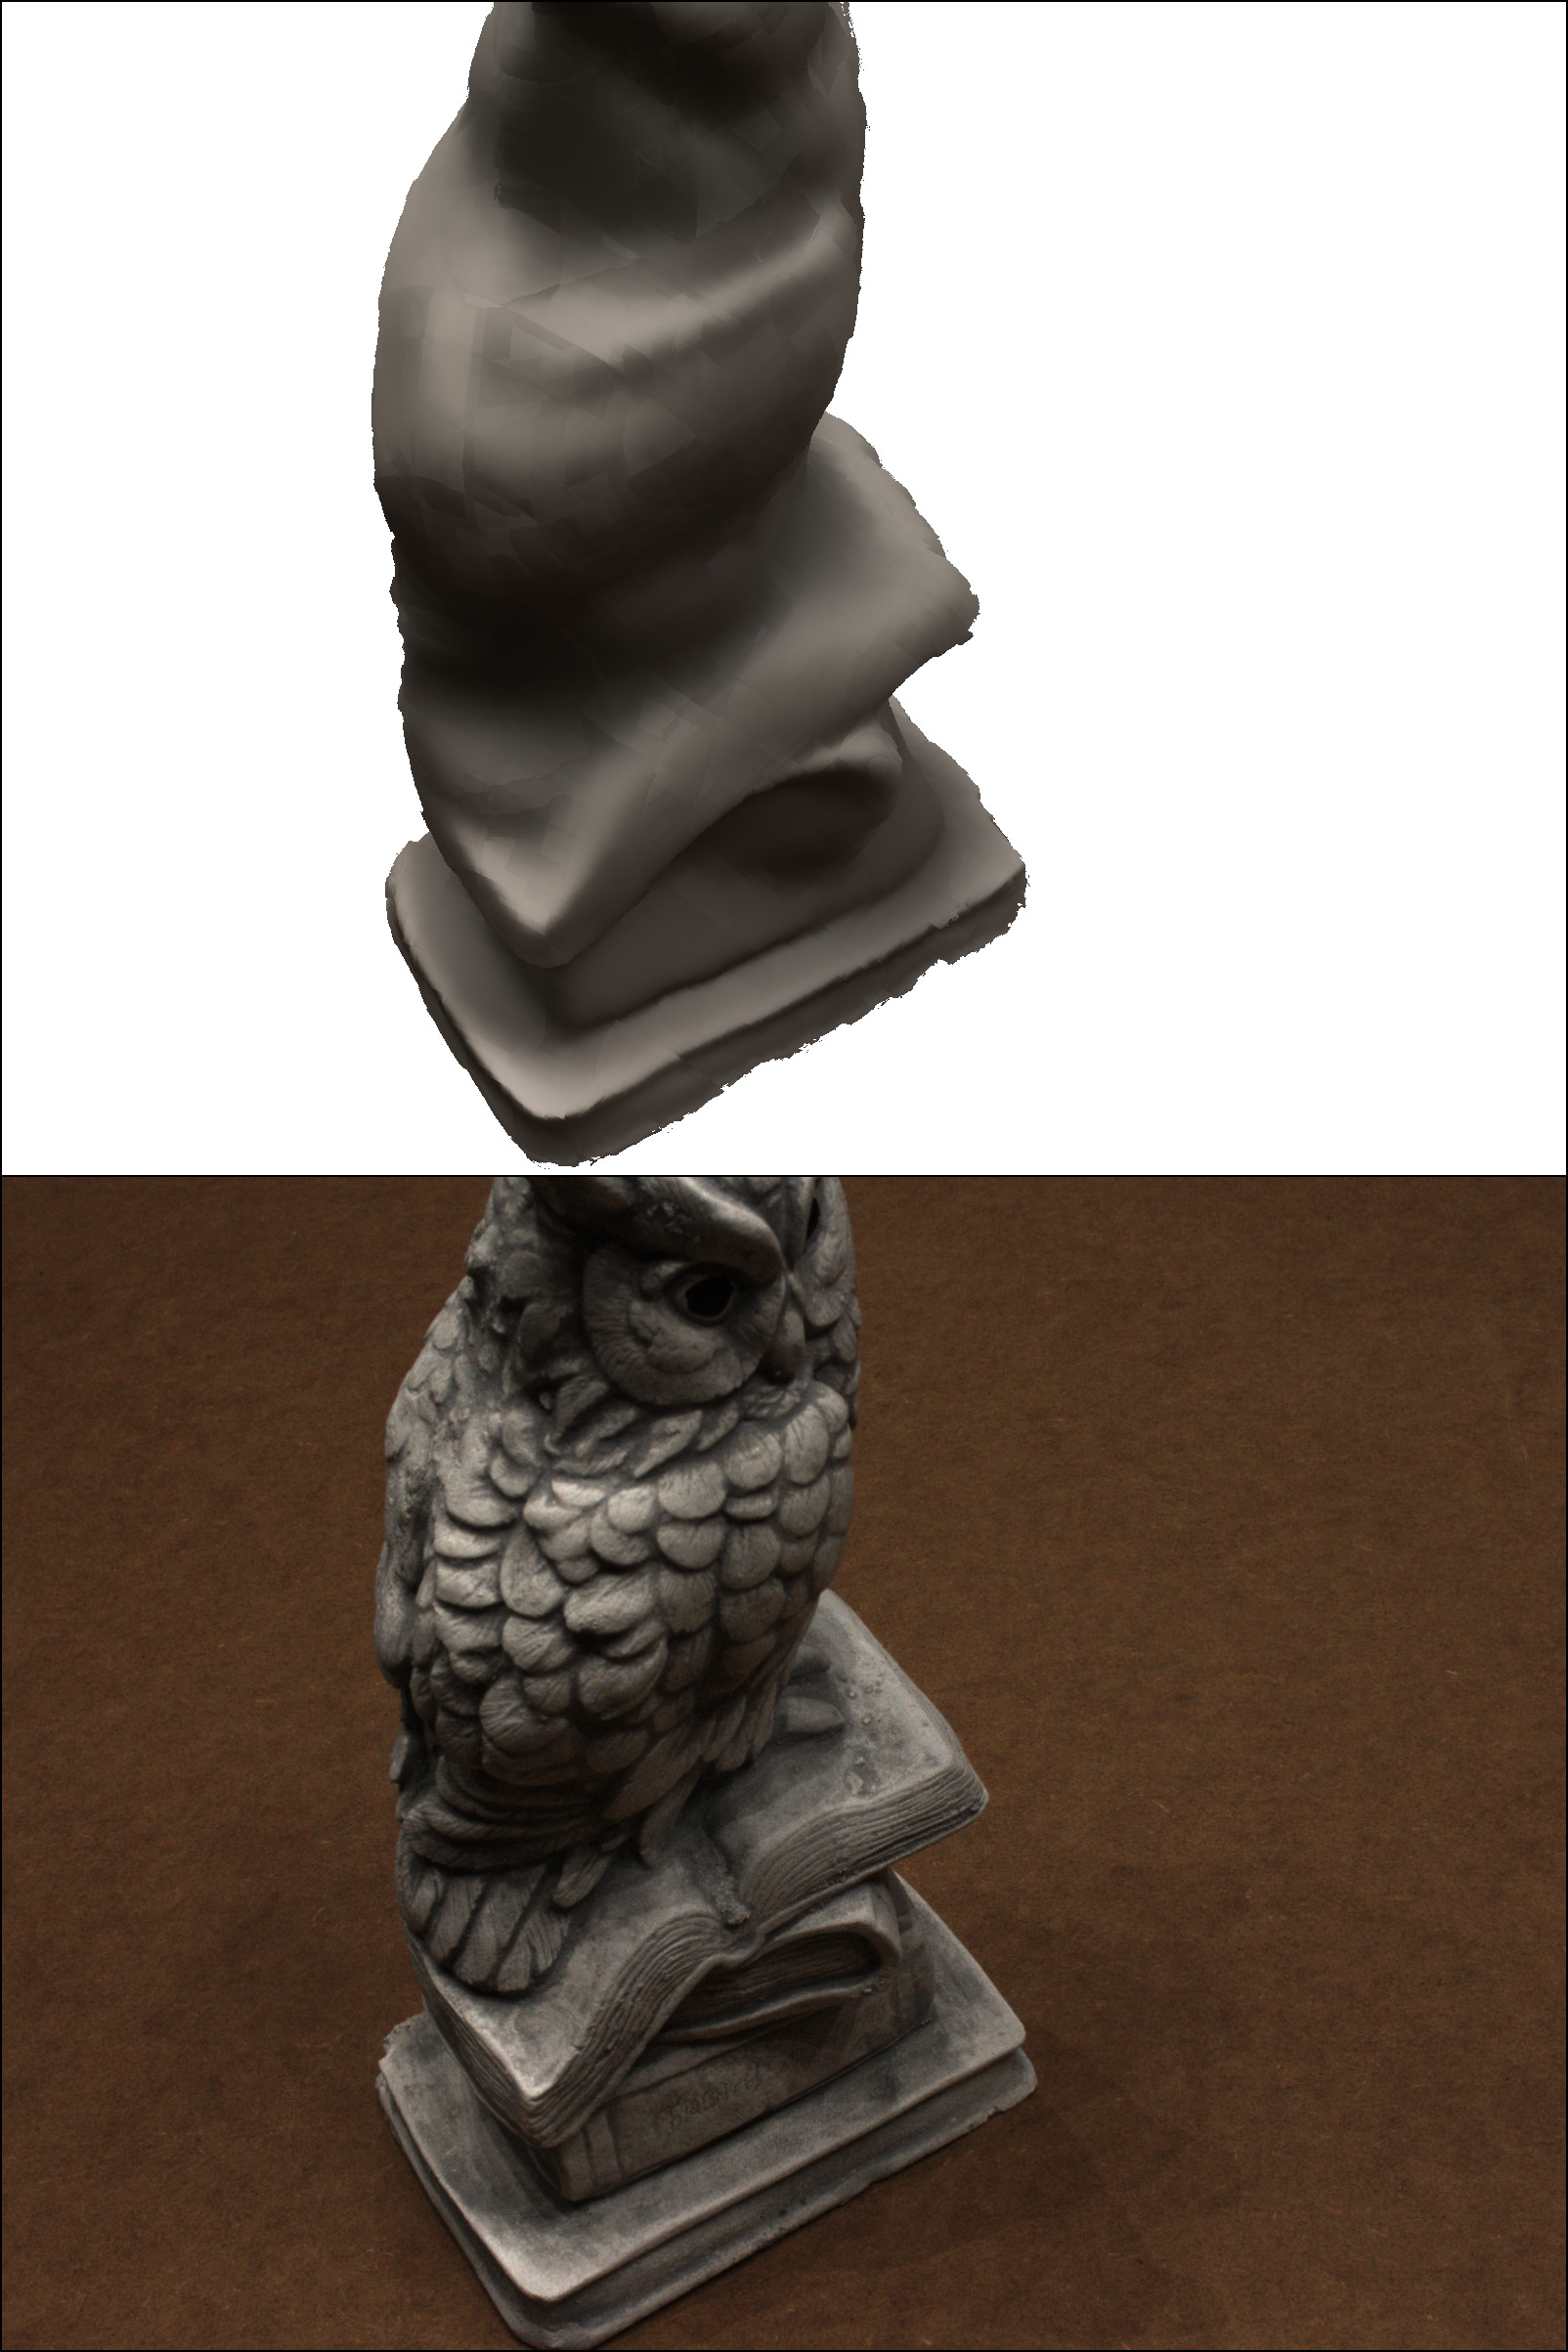
\includegraphics[width=1.5cm]{images/chapter5_img/RenderedImages-DepthMaps-EpochWise-Evals/MRHashGrid3D/122/rendering_100.jpg} & 
    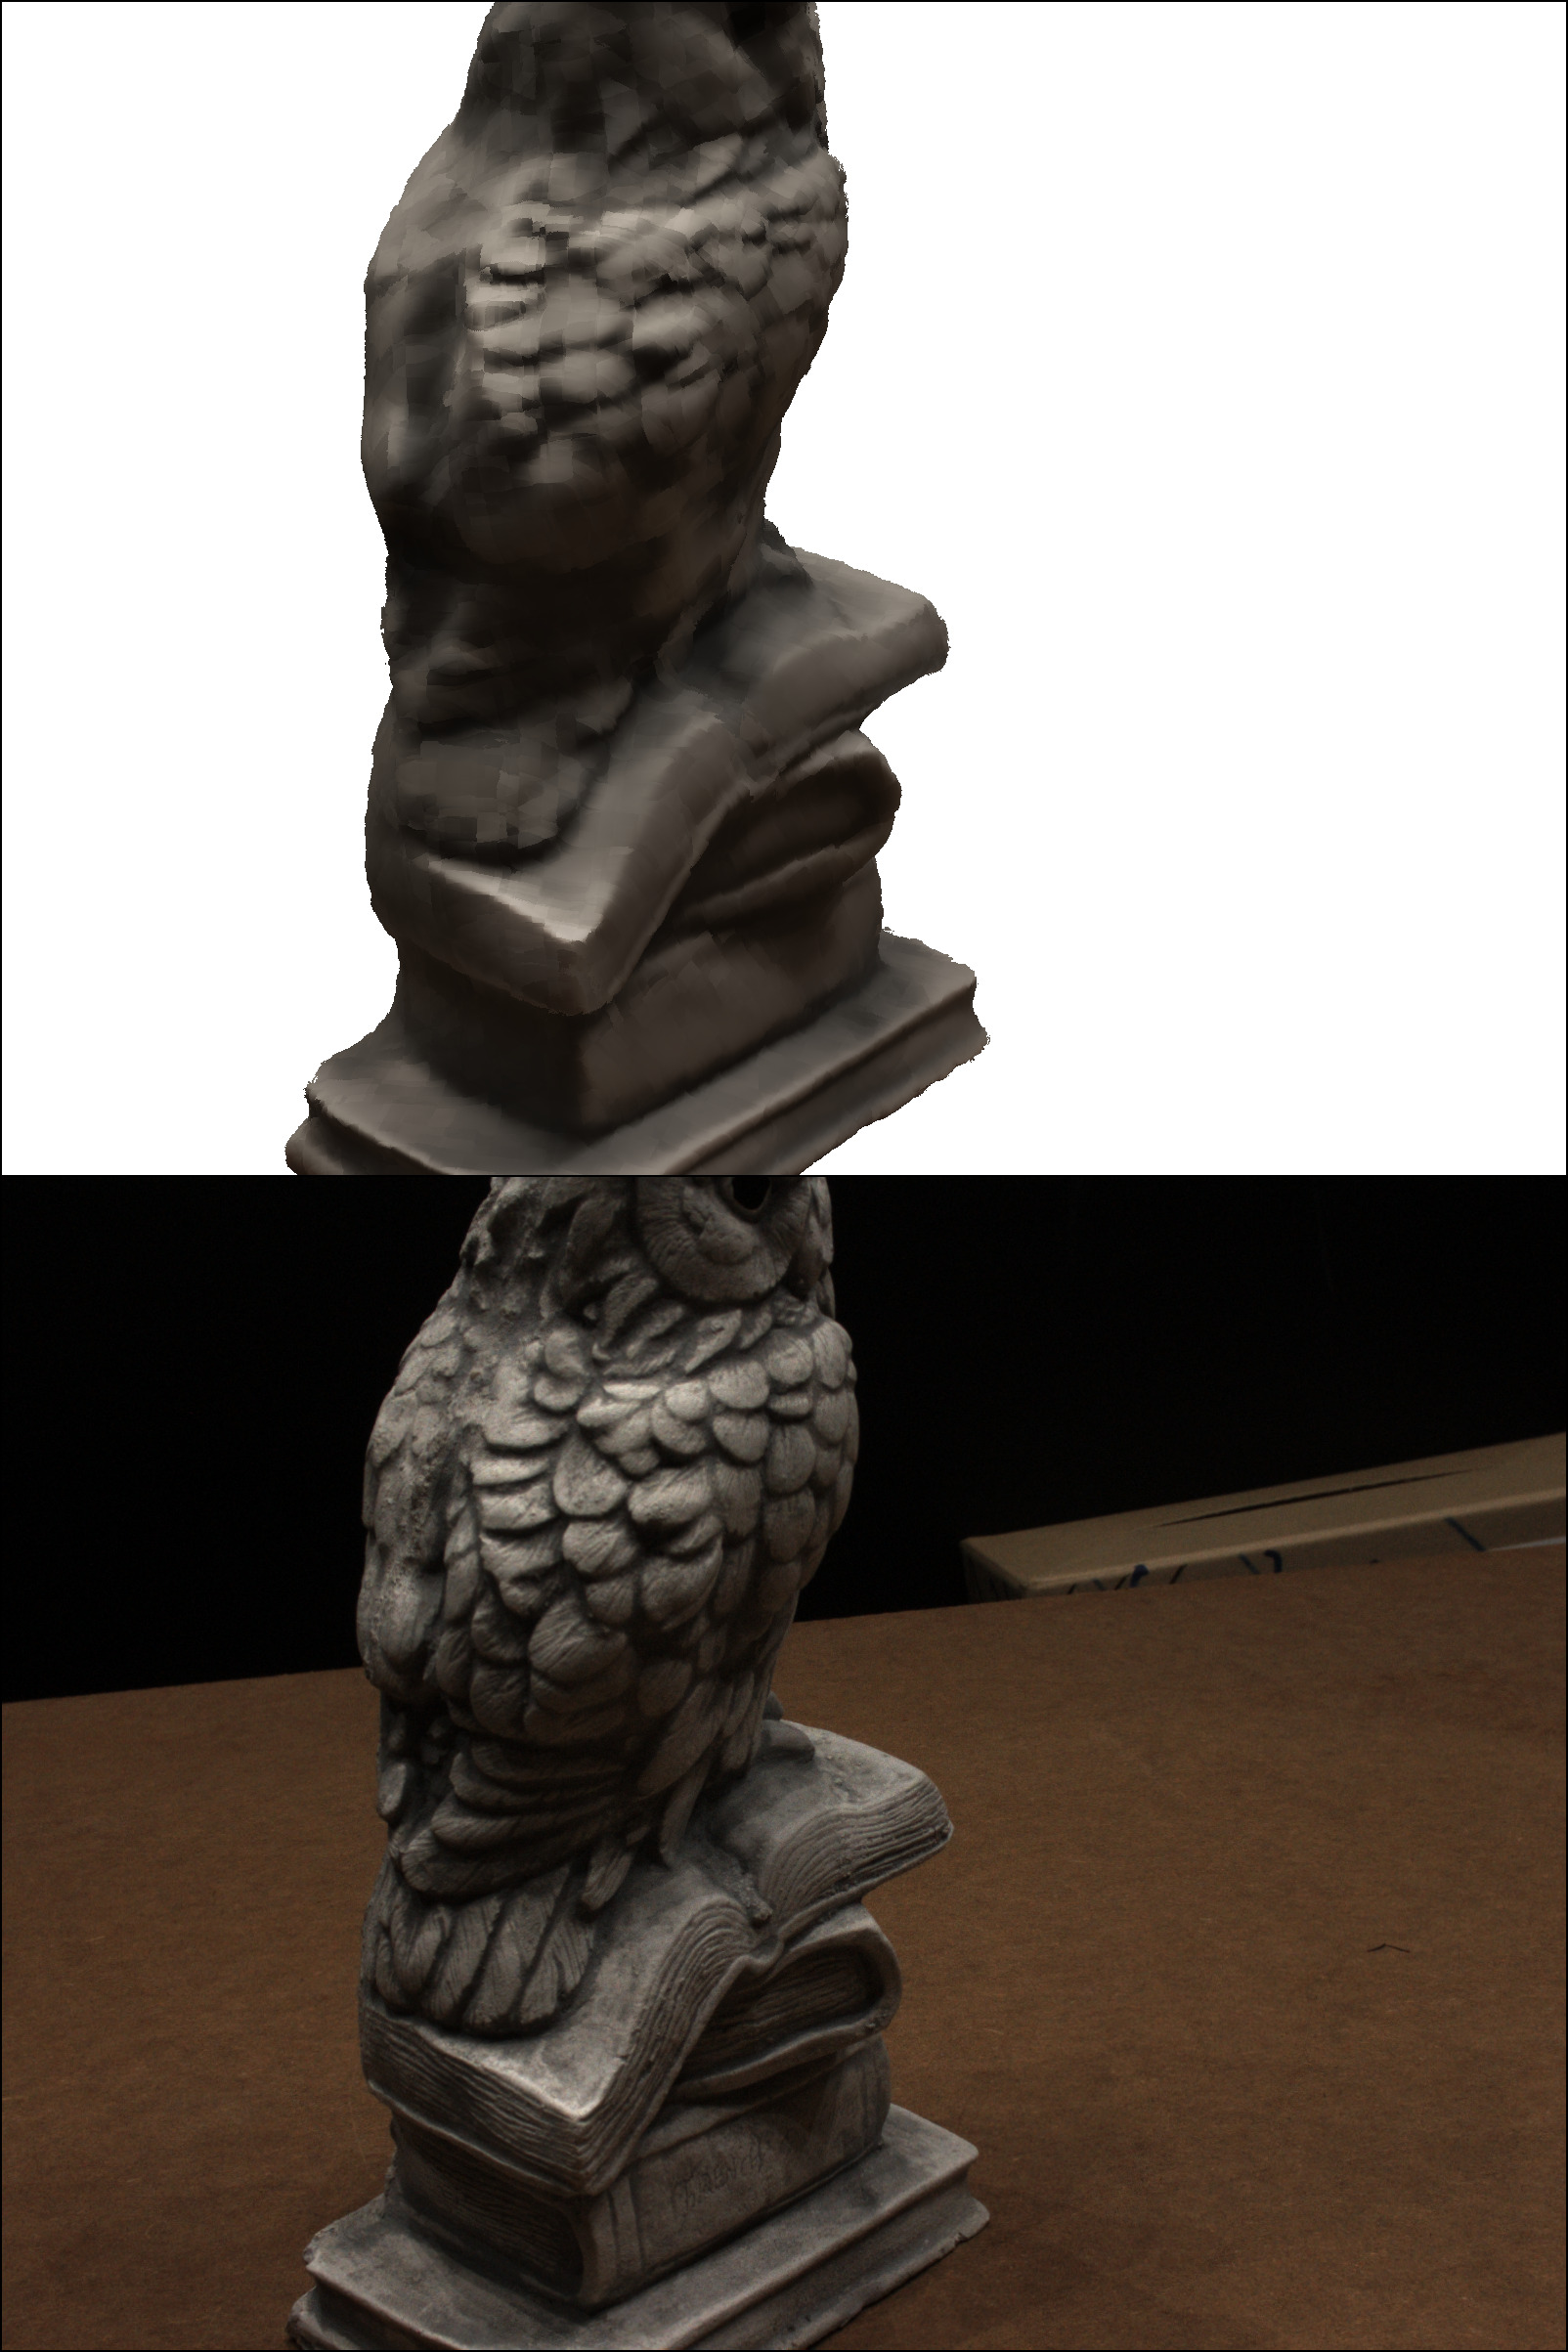
\includegraphics[width=1.5cm]{images/chapter5_img/RenderedImages-DepthMaps-EpochWise-Evals/MRHashGrid3D/122/rendering_500.jpg} & 
    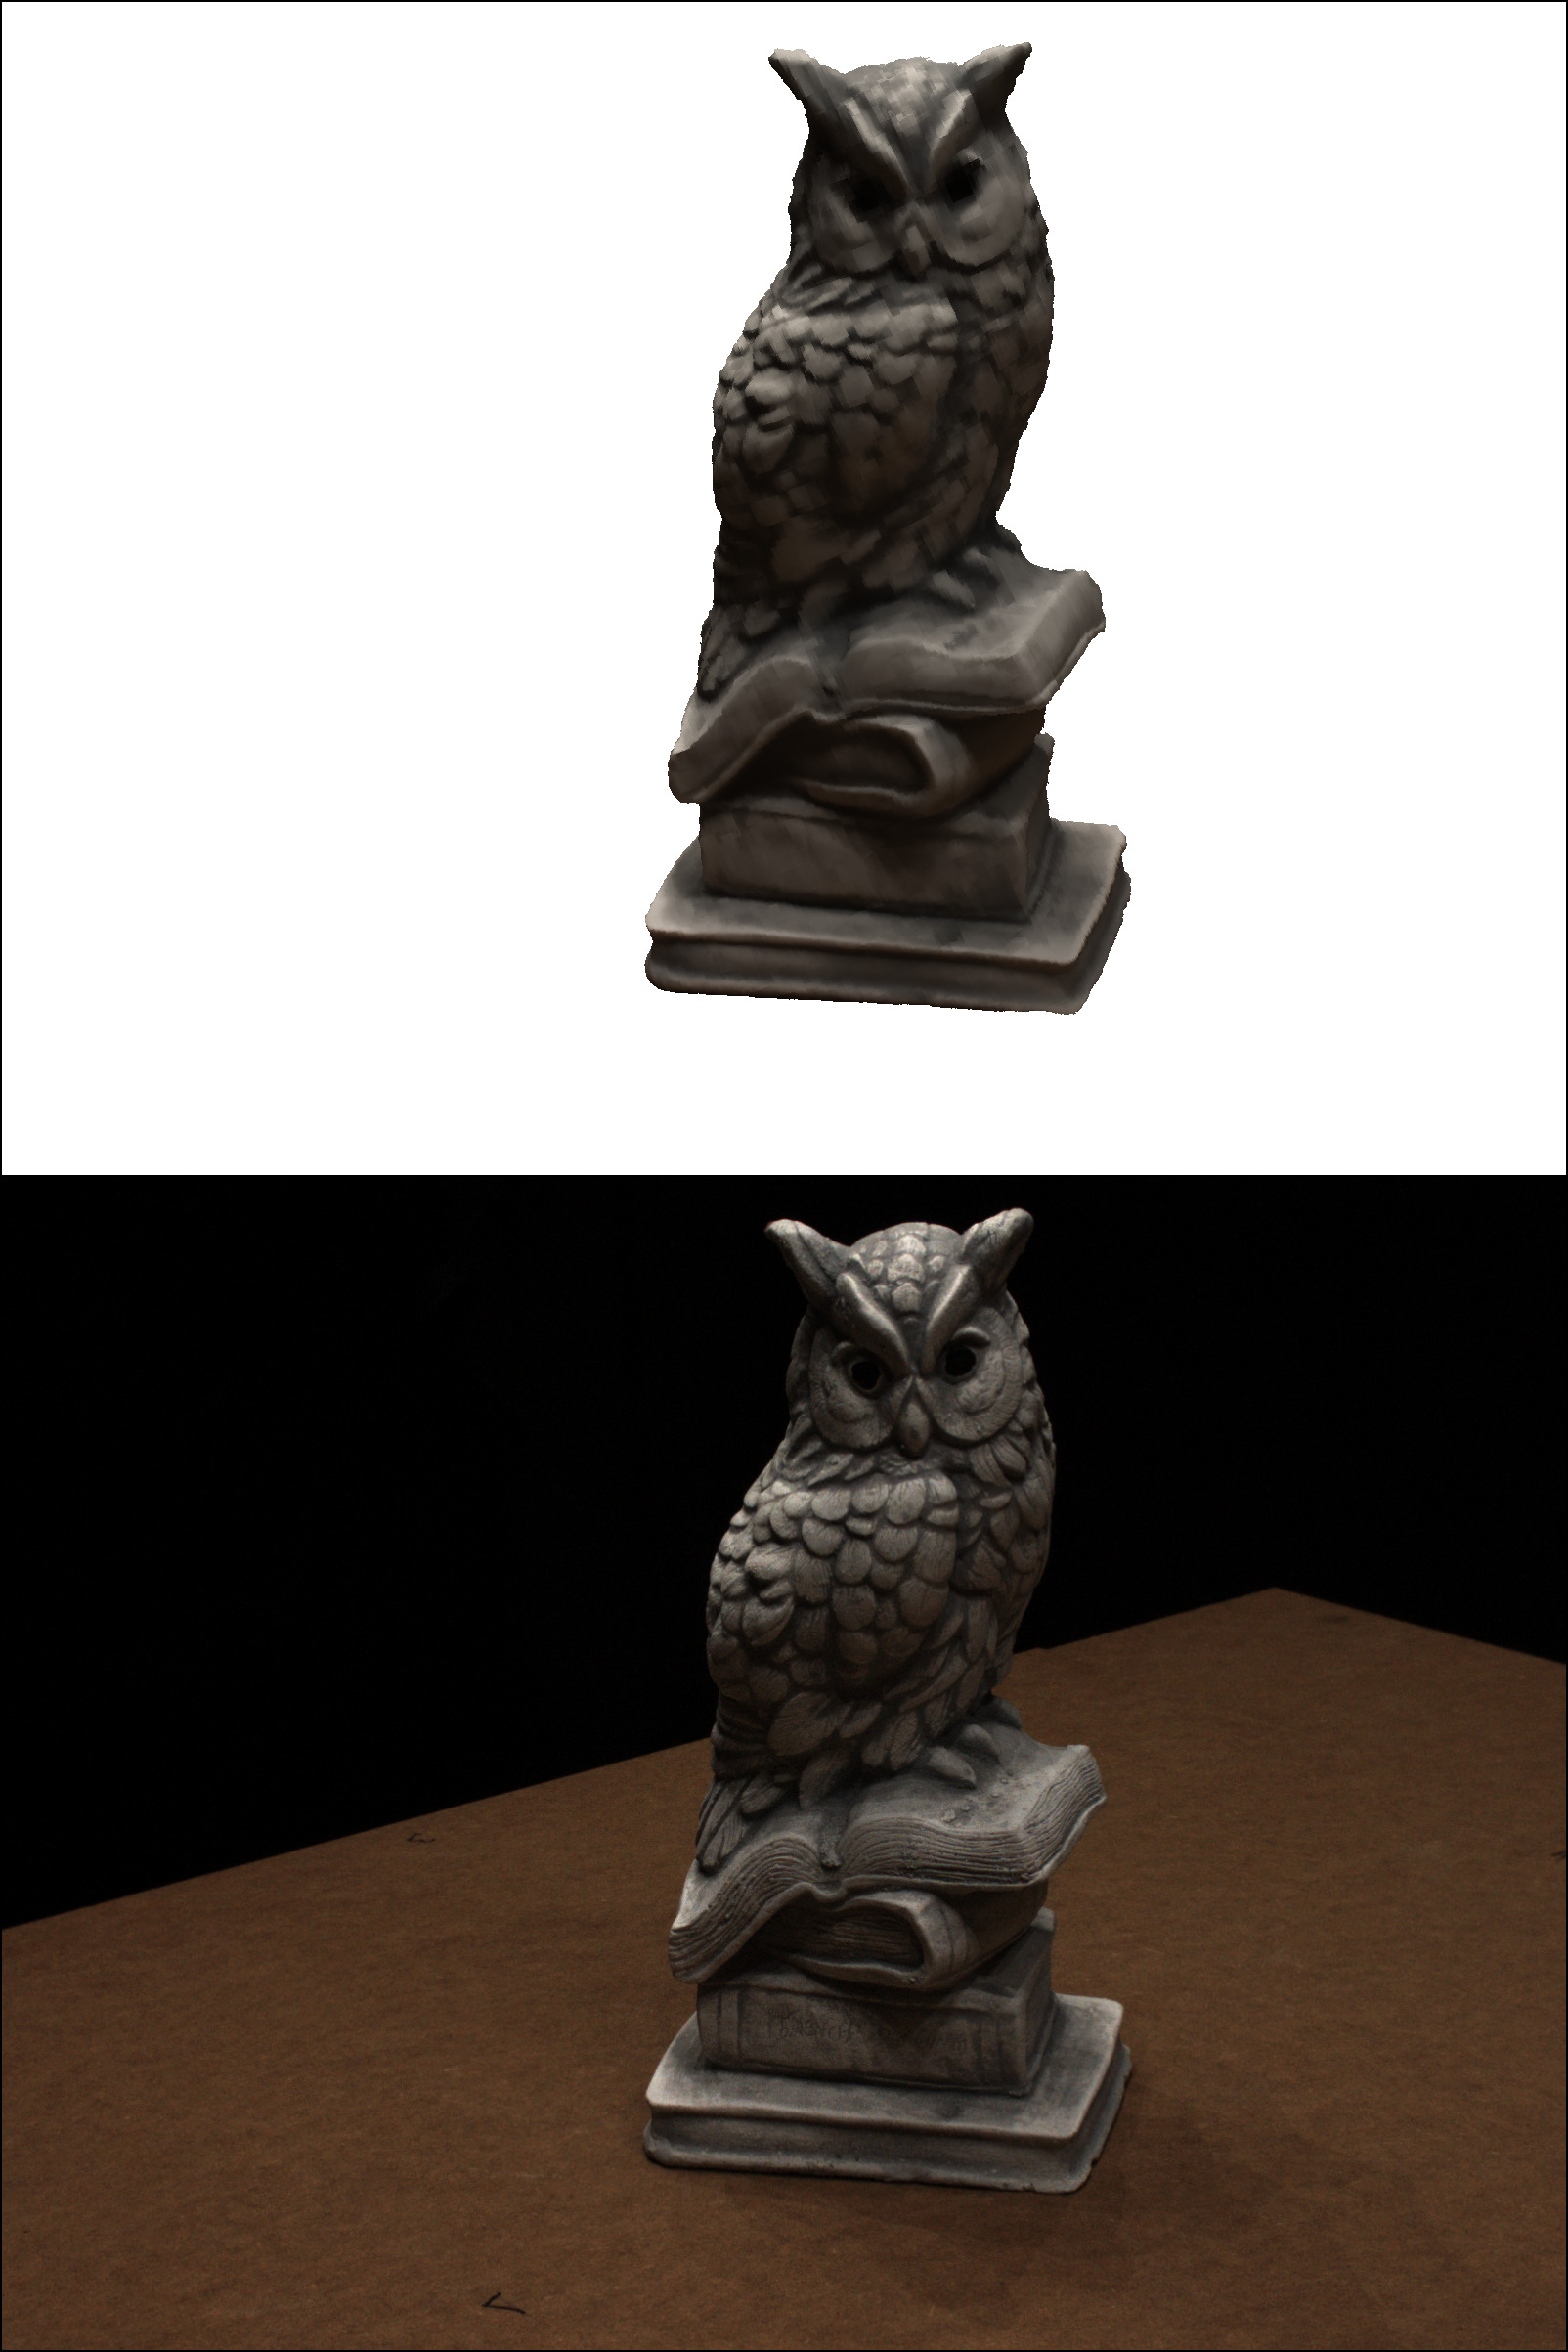
\includegraphics[width=1.5cm]{images/chapter5_img/RenderedImages-DepthMaps-EpochWise-Evals/MRHashGrid3D/122/rendering_1000.jpg} & 
    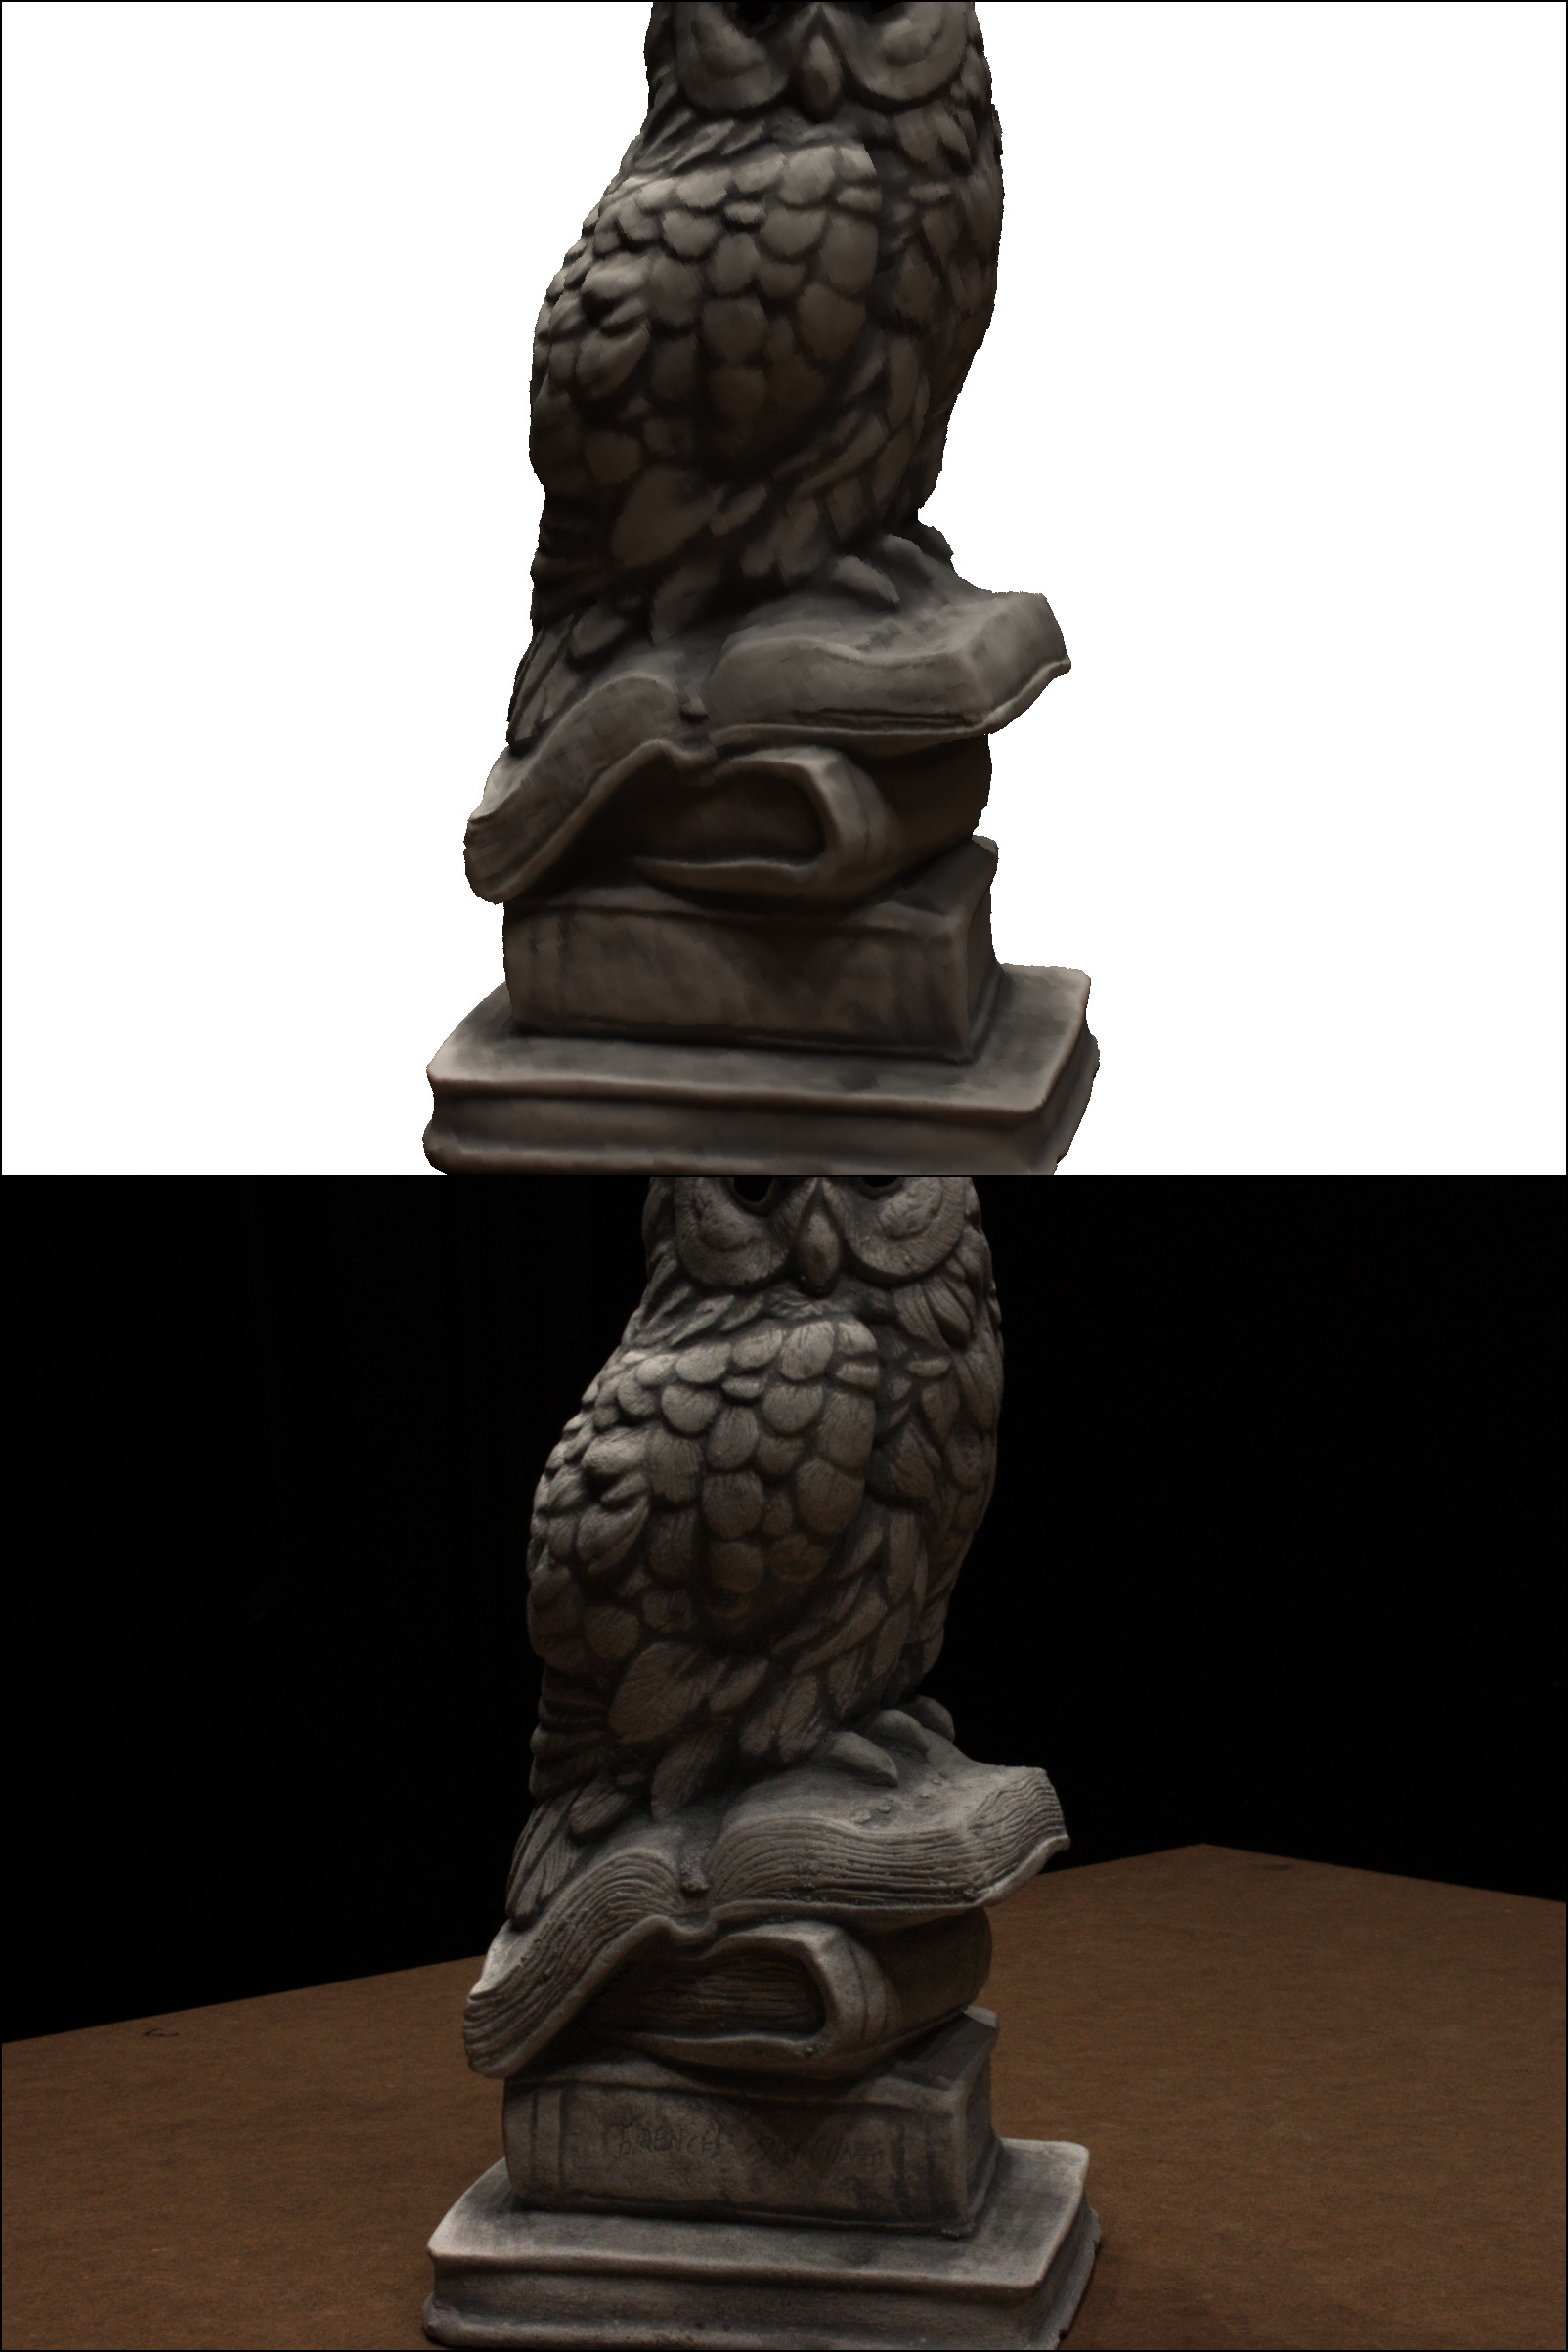
\includegraphics[width=1.5cm]{images/chapter5_img/RenderedImages-DepthMaps-EpochWise-Evals/MRHashGrid3D/122/rendering_2000.jpg} & 
    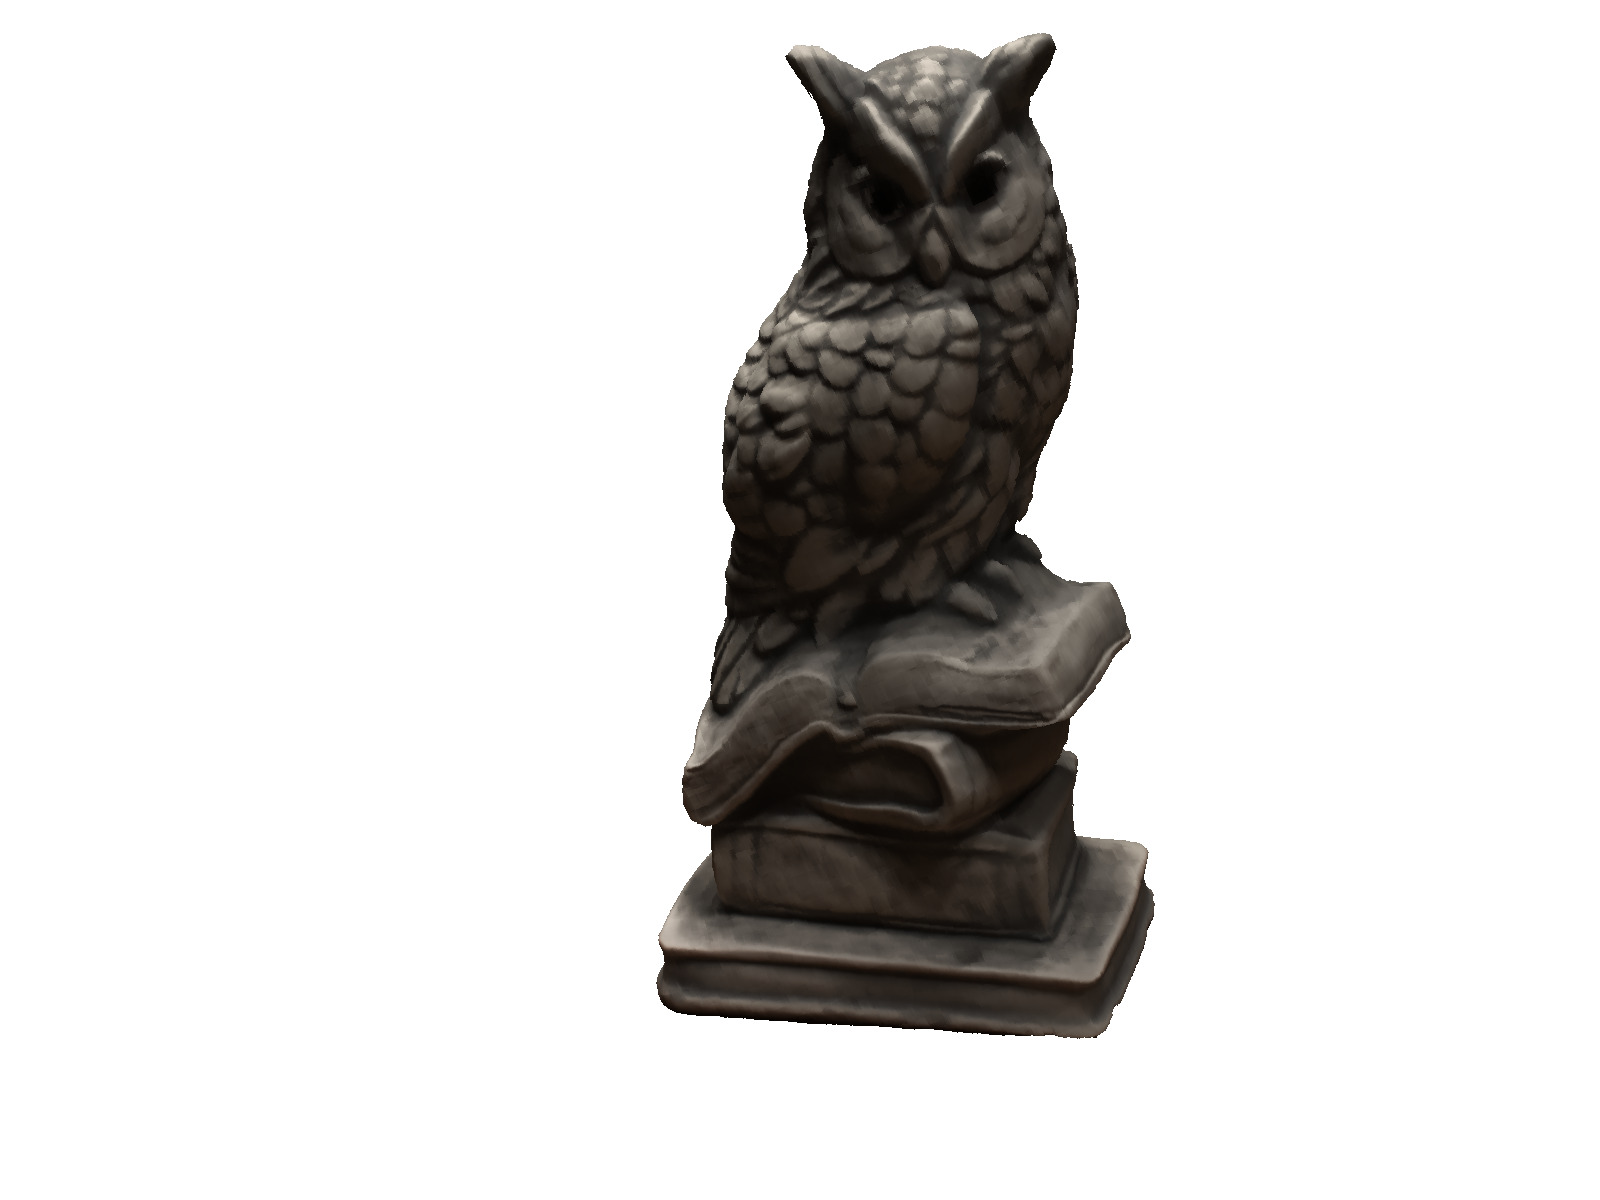
\includegraphics[width=1.5cm]{images/chapter5_img/RenderedImages-DepthMaps-EpochWise-Evals/MRHashGrid3D/122/eval_055.jpg} \\
    \hline 
    NFFB & 
    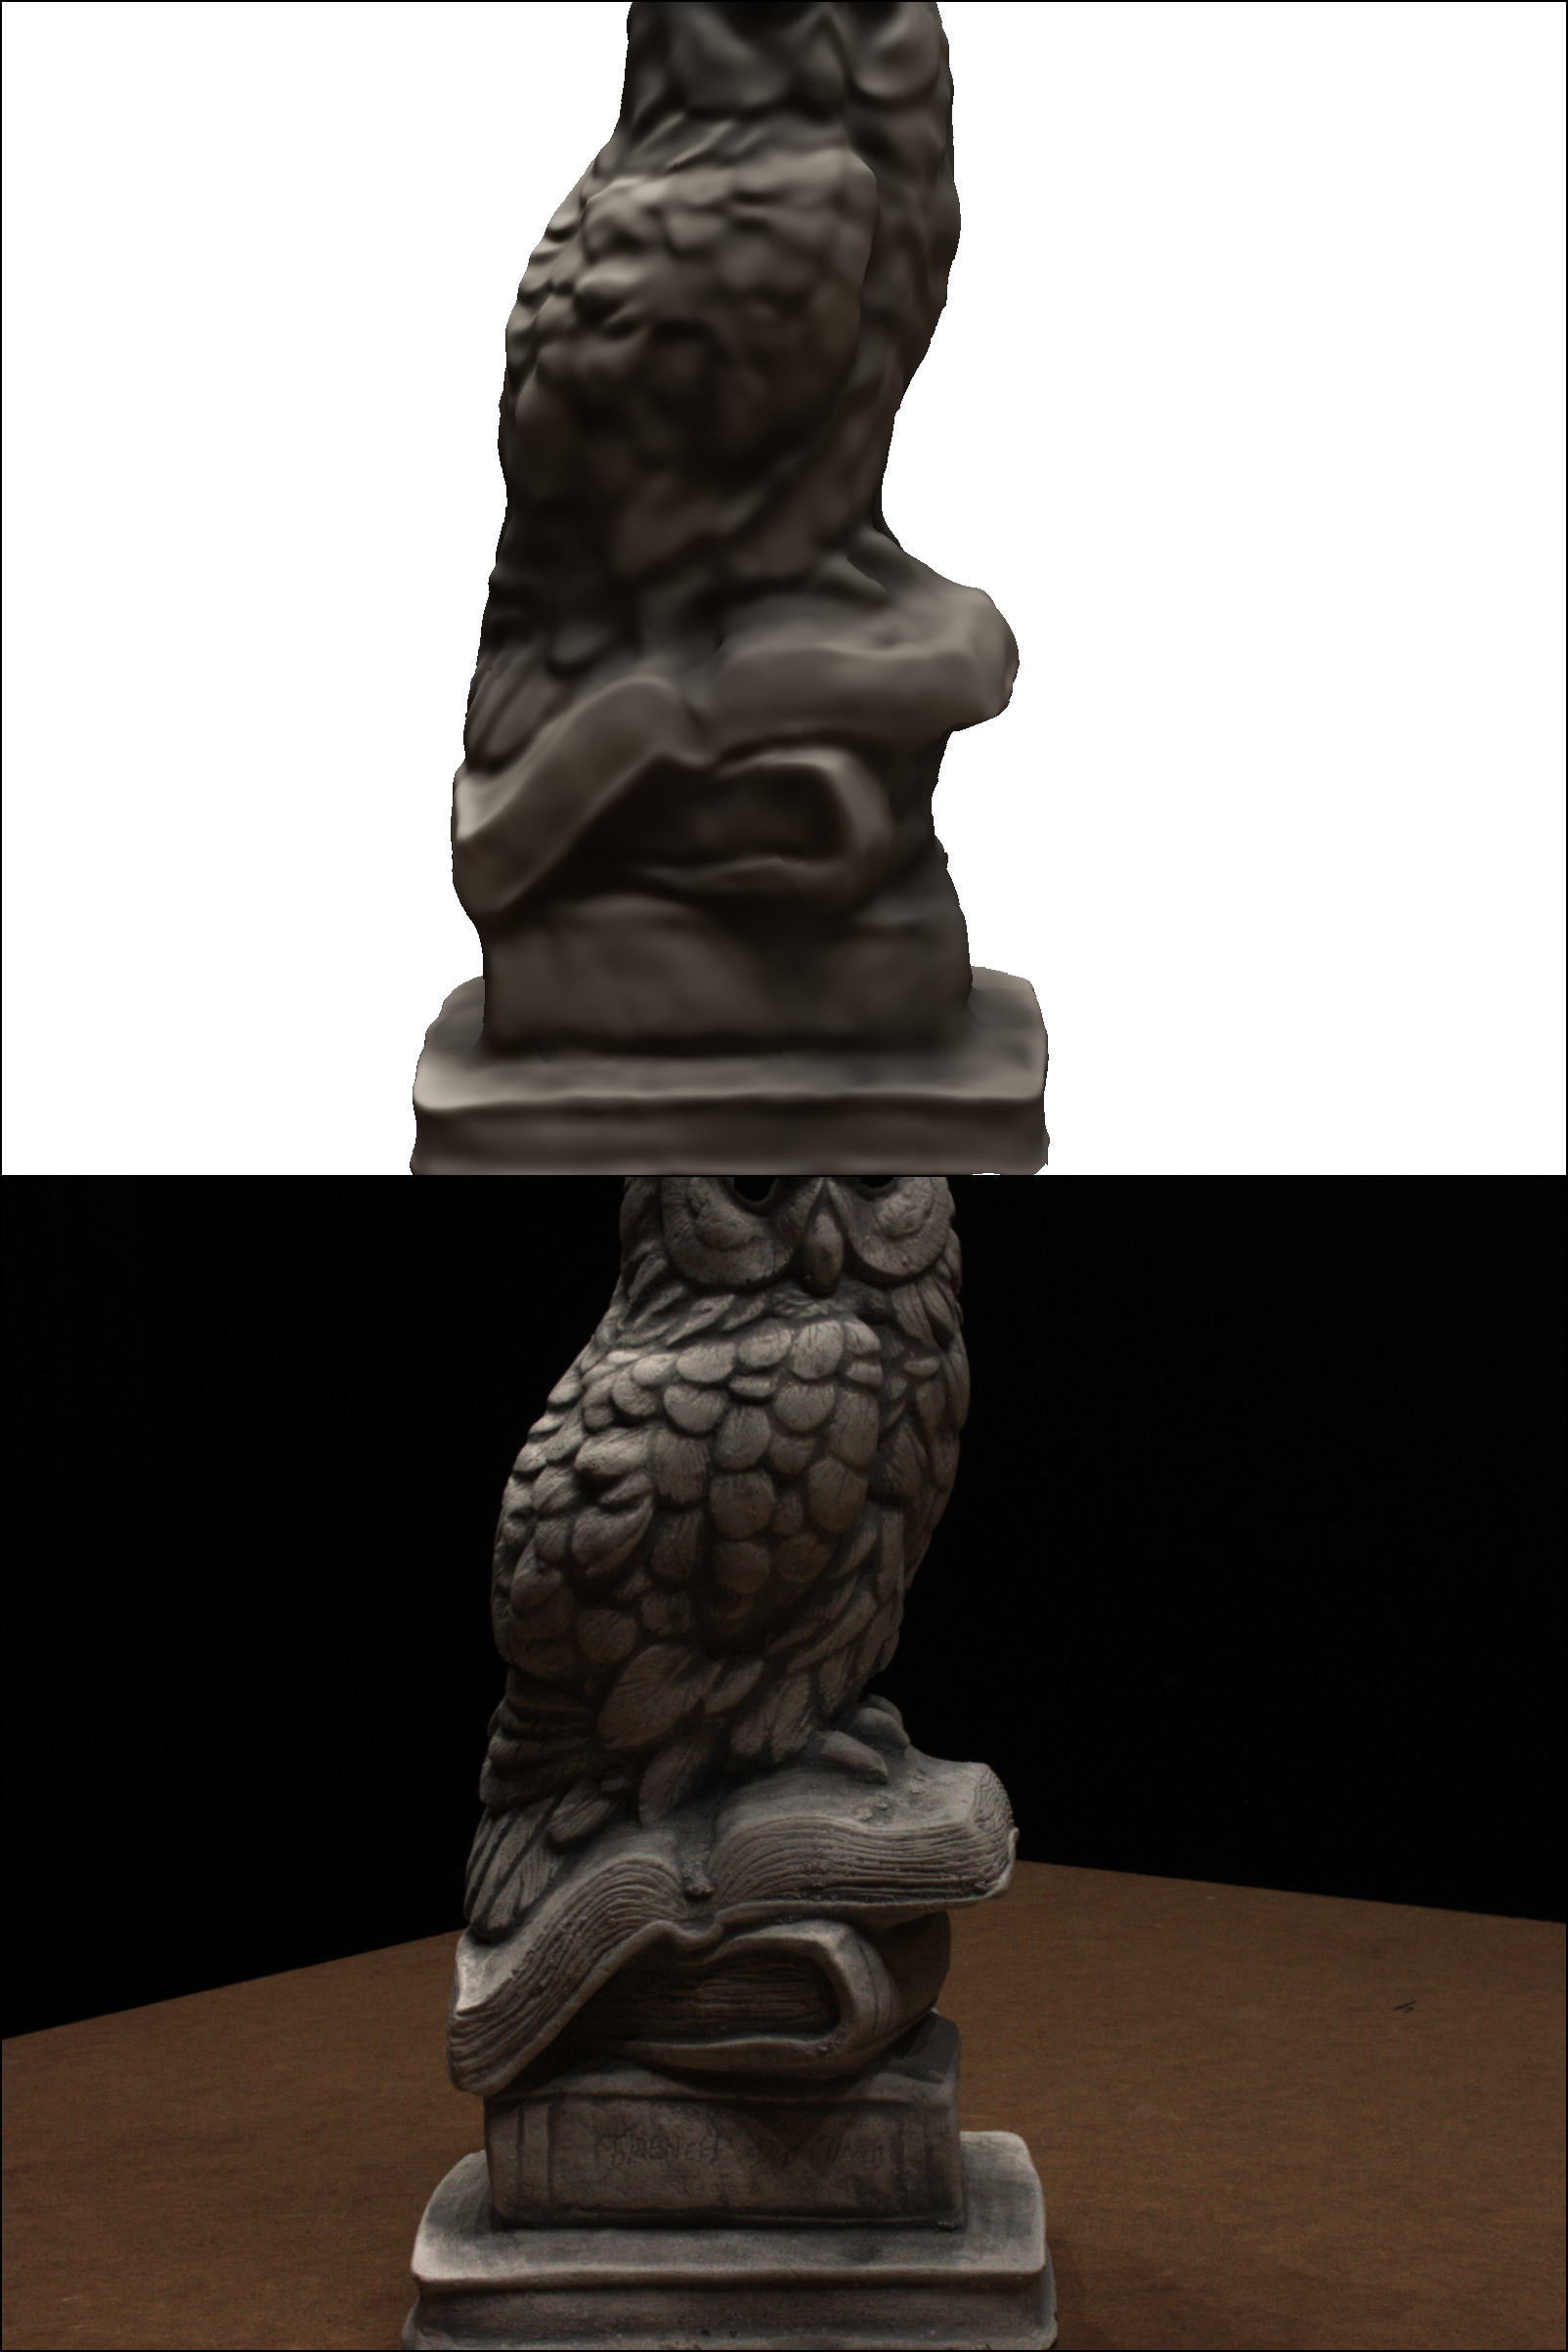
\includegraphics[width=1.5cm]{images/chapter5_img/RenderedImages-DepthMaps-EpochWise-Evals/NFFB/122/rendering_100.jpg} & 
    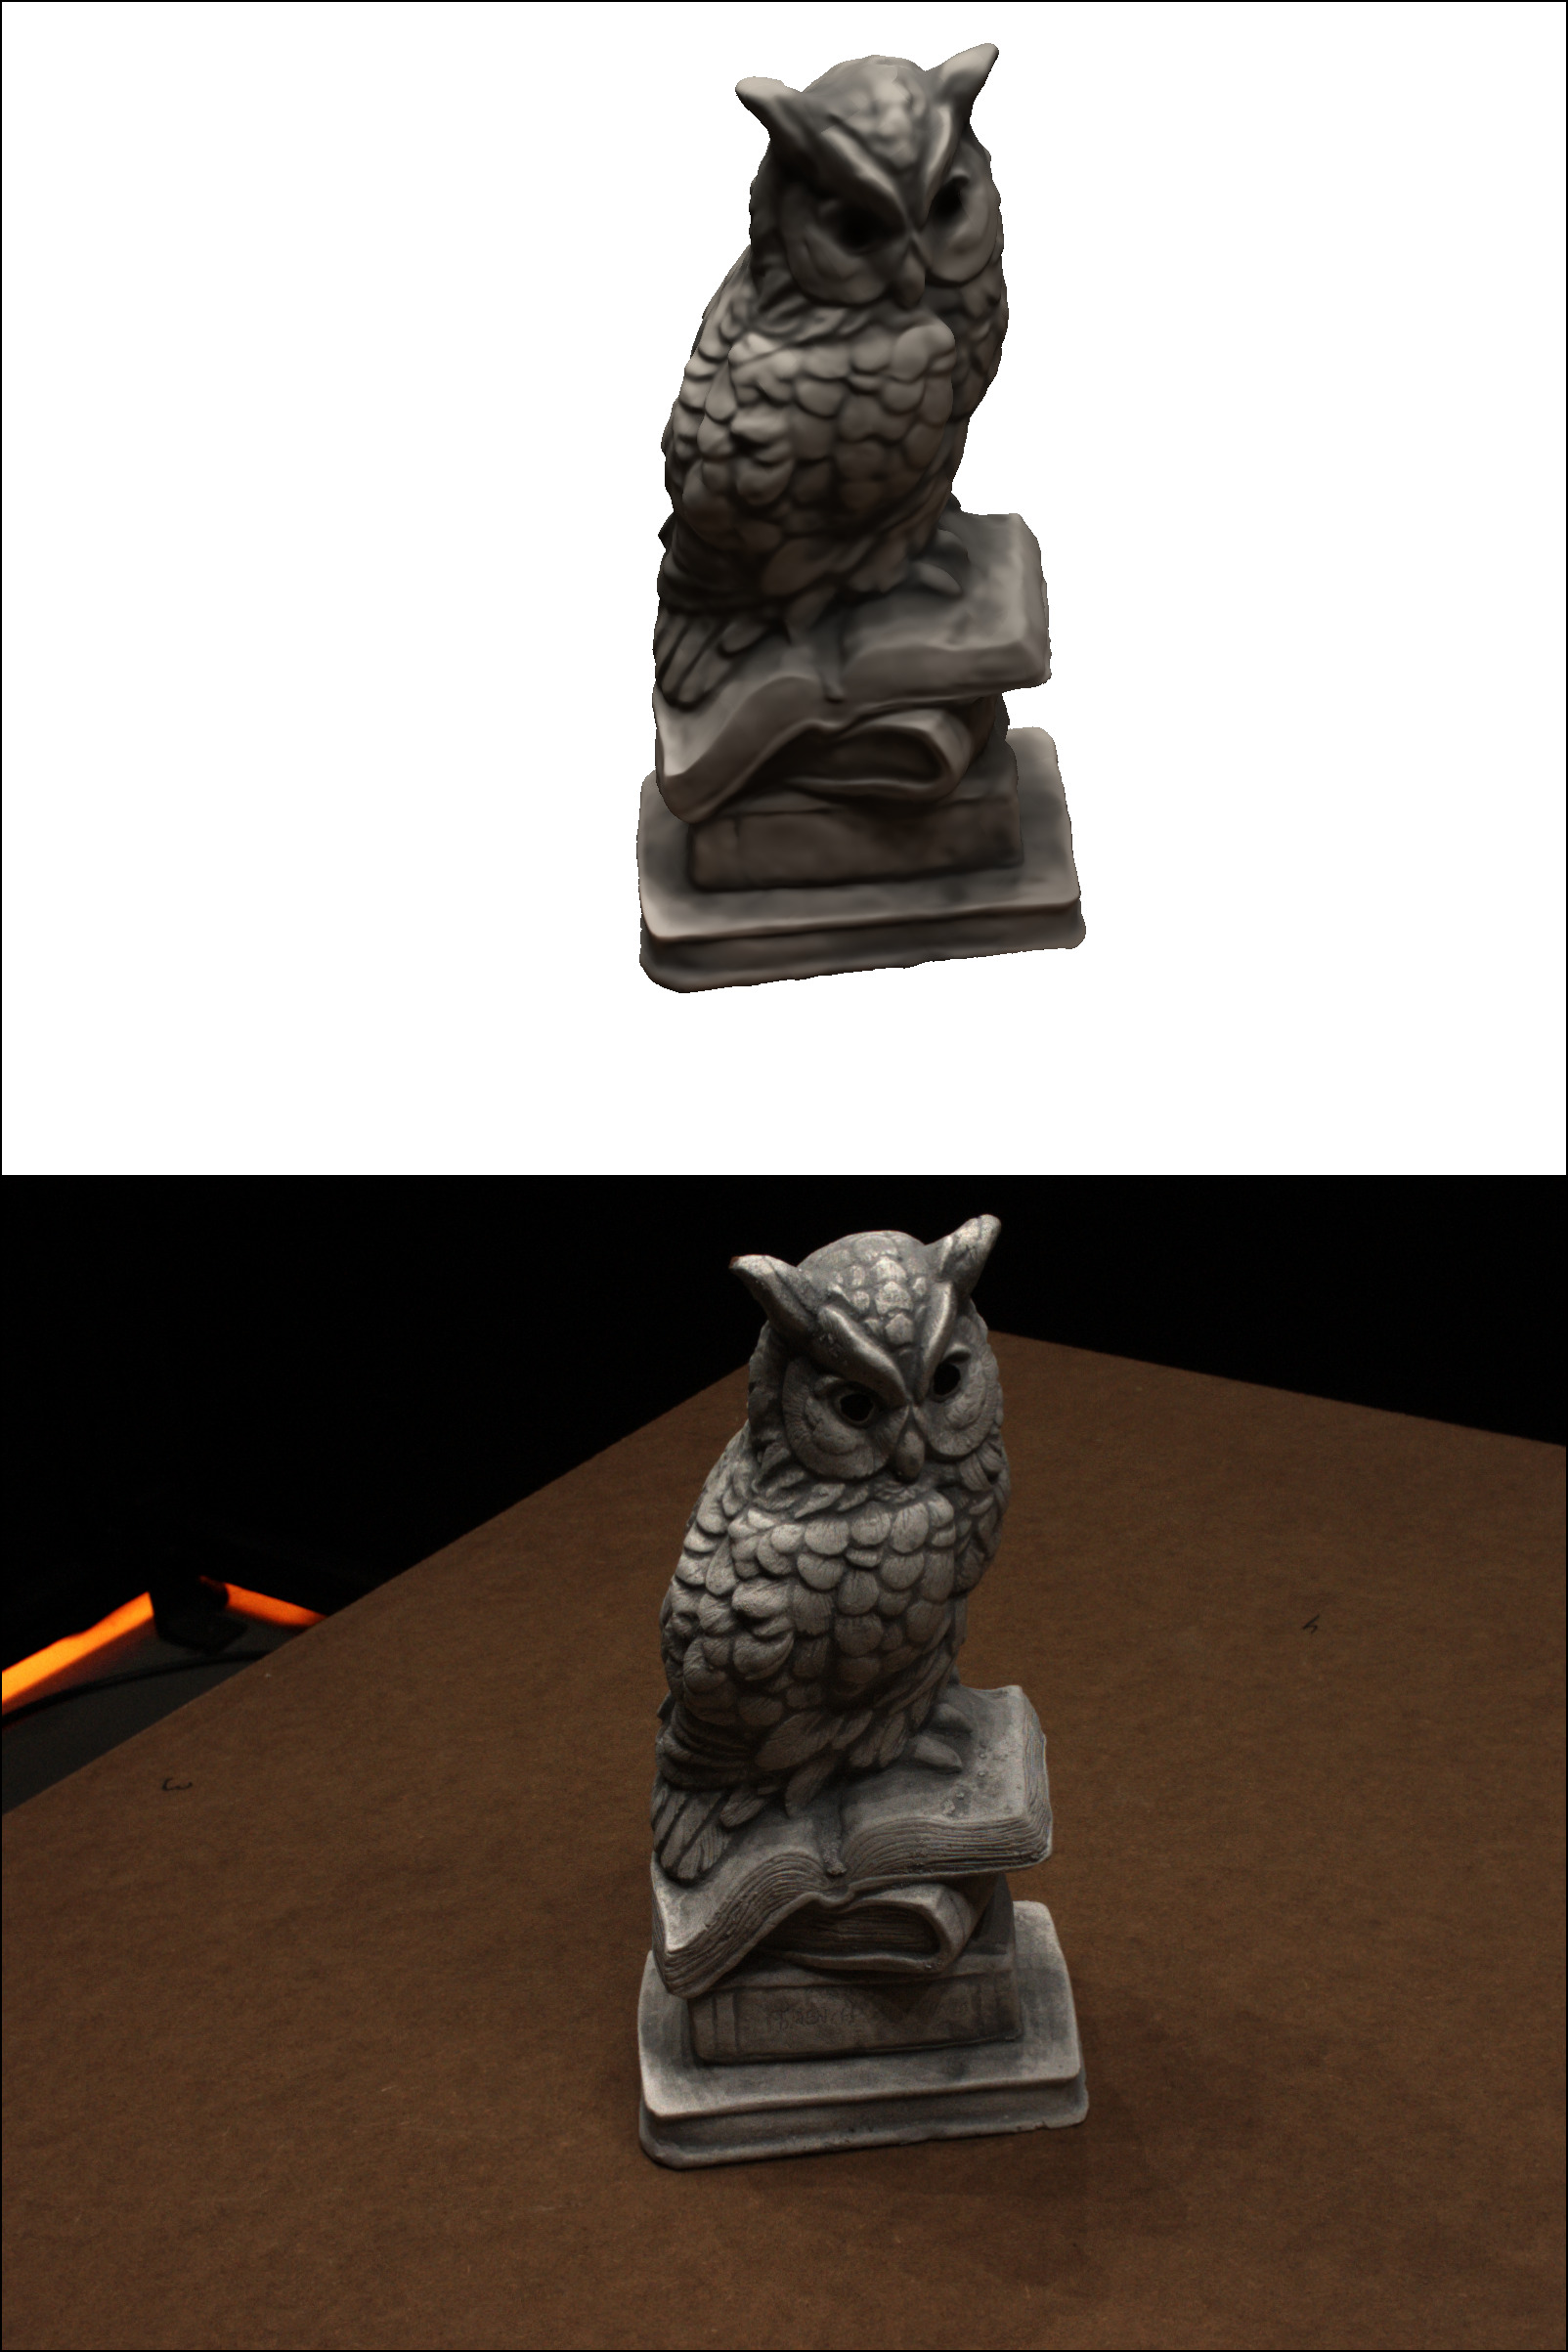
\includegraphics[width=1.5cm]{images/chapter5_img/RenderedImages-DepthMaps-EpochWise-Evals/NFFB/122/rendering_500.jpg} & 
    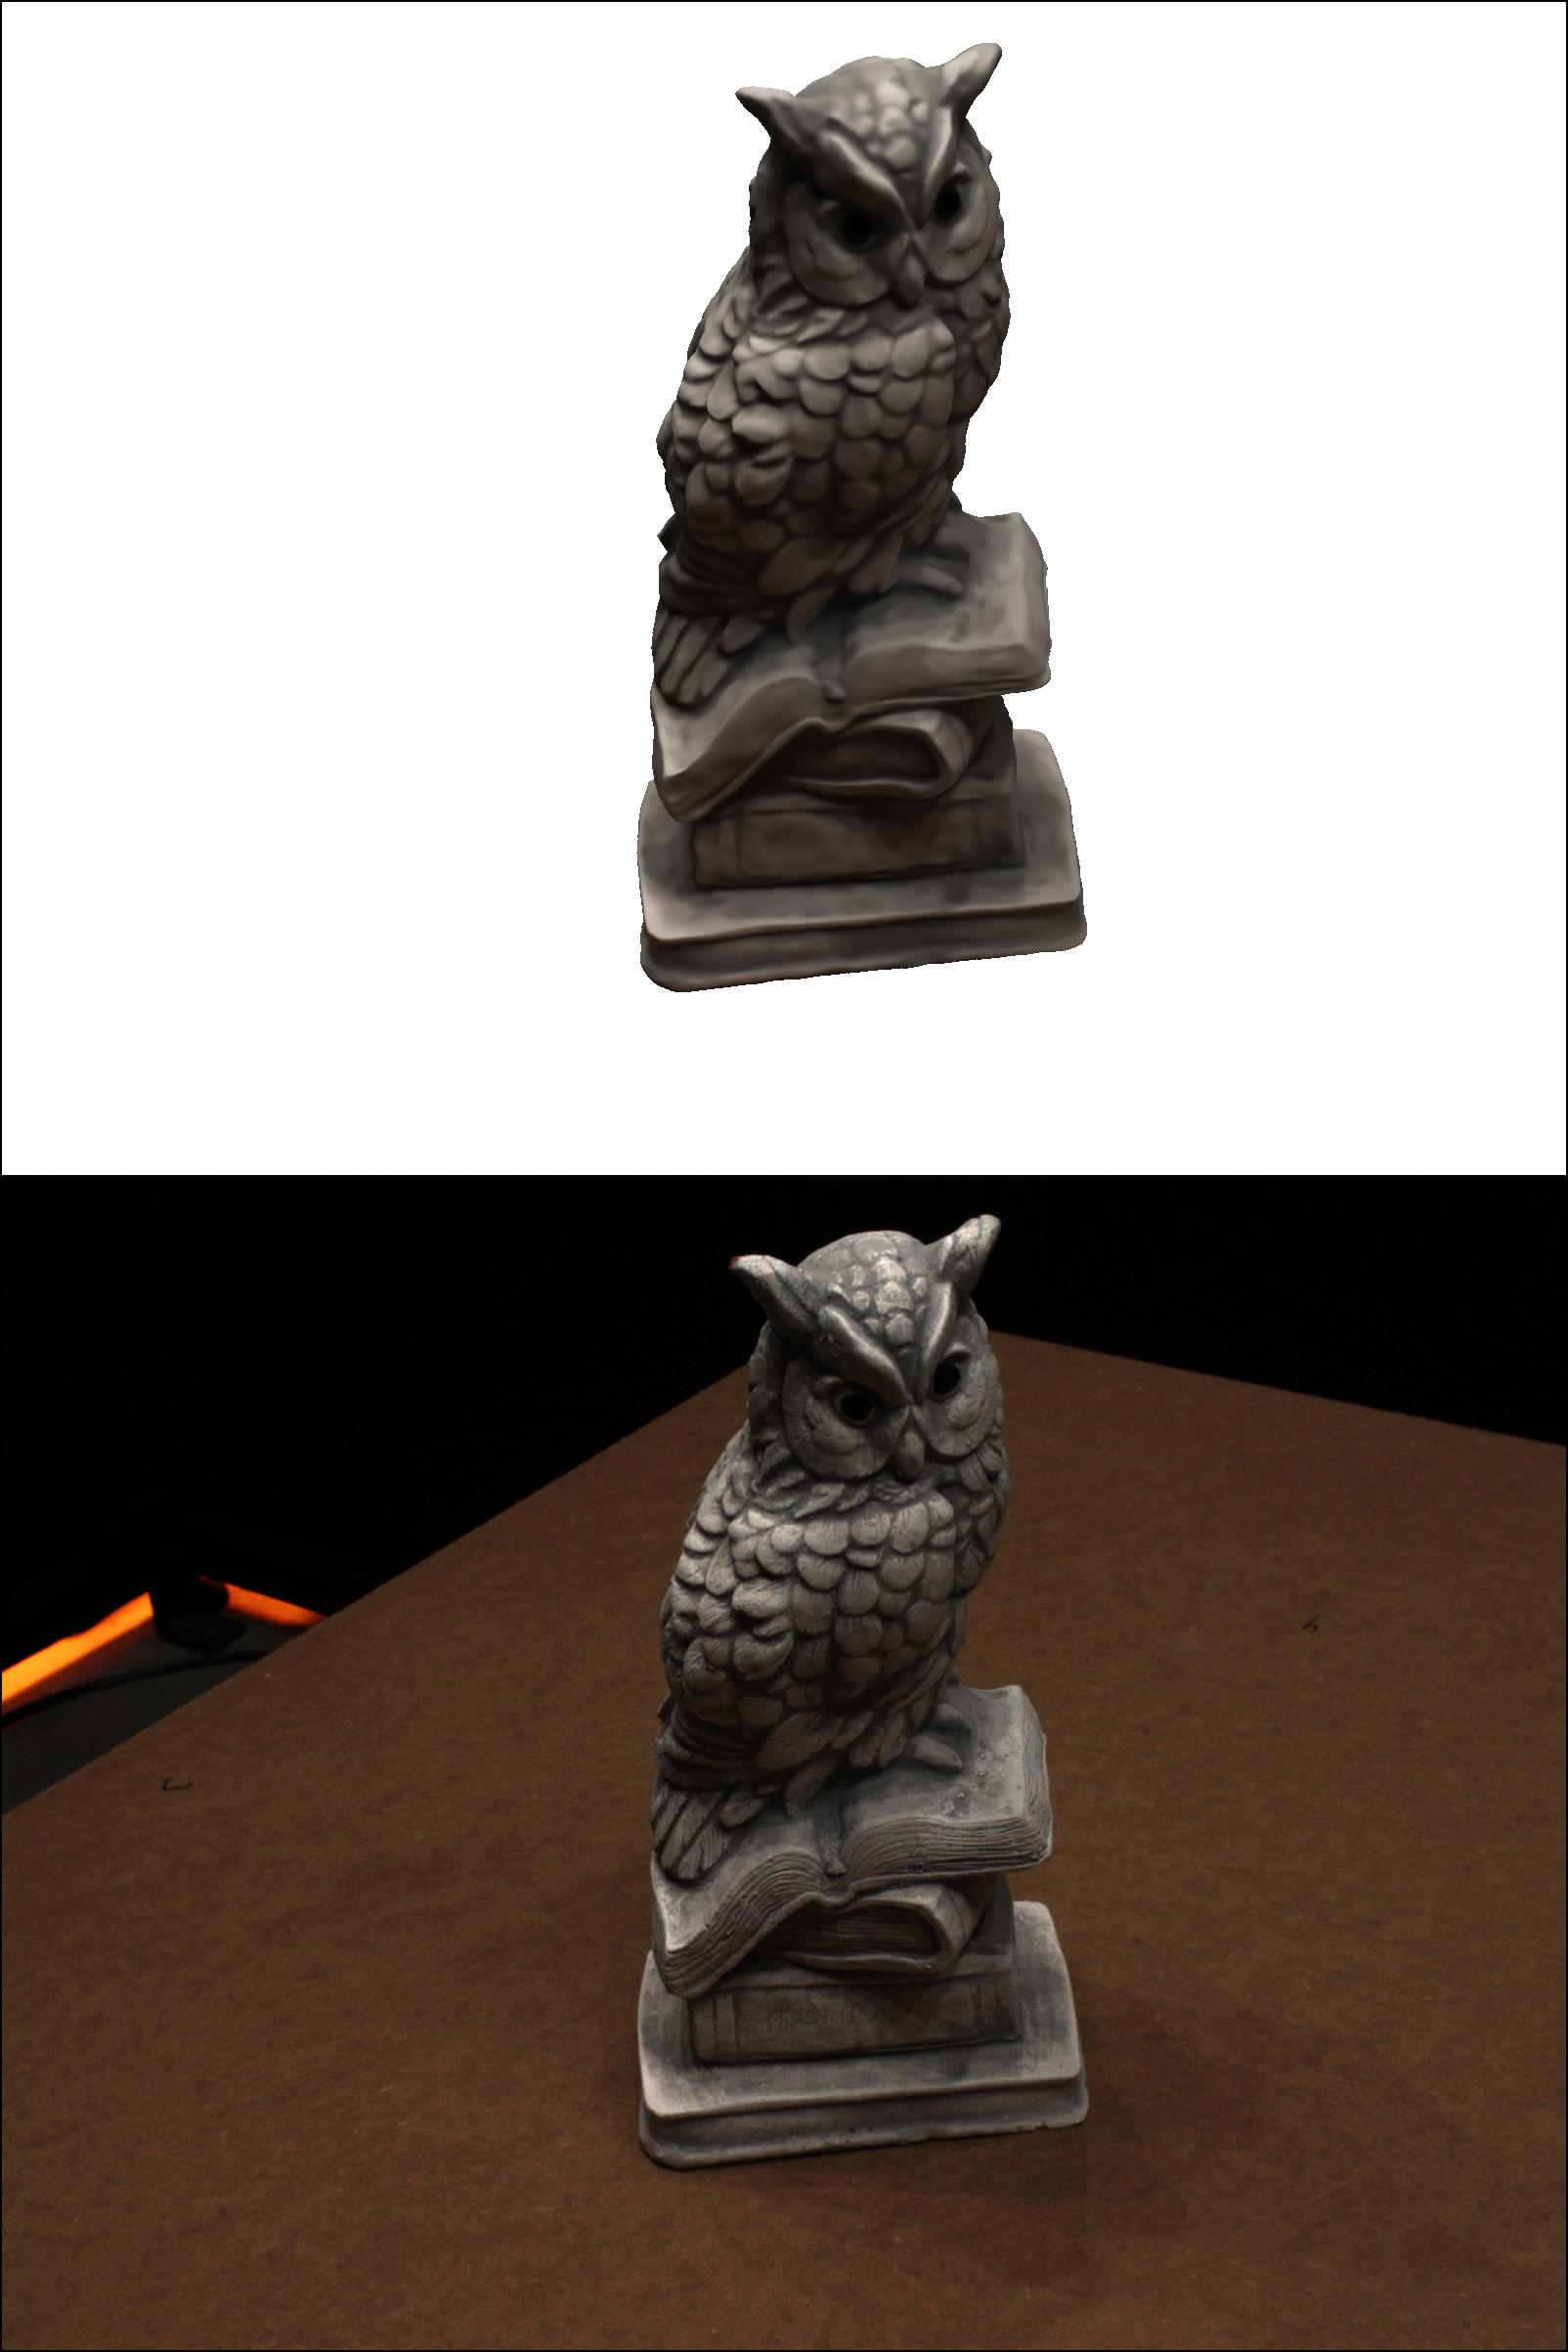
\includegraphics[width=1.5cm]{images/chapter5_img/RenderedImages-DepthMaps-EpochWise-Evals/NFFB/122/rendering_1000.jpg} & 
    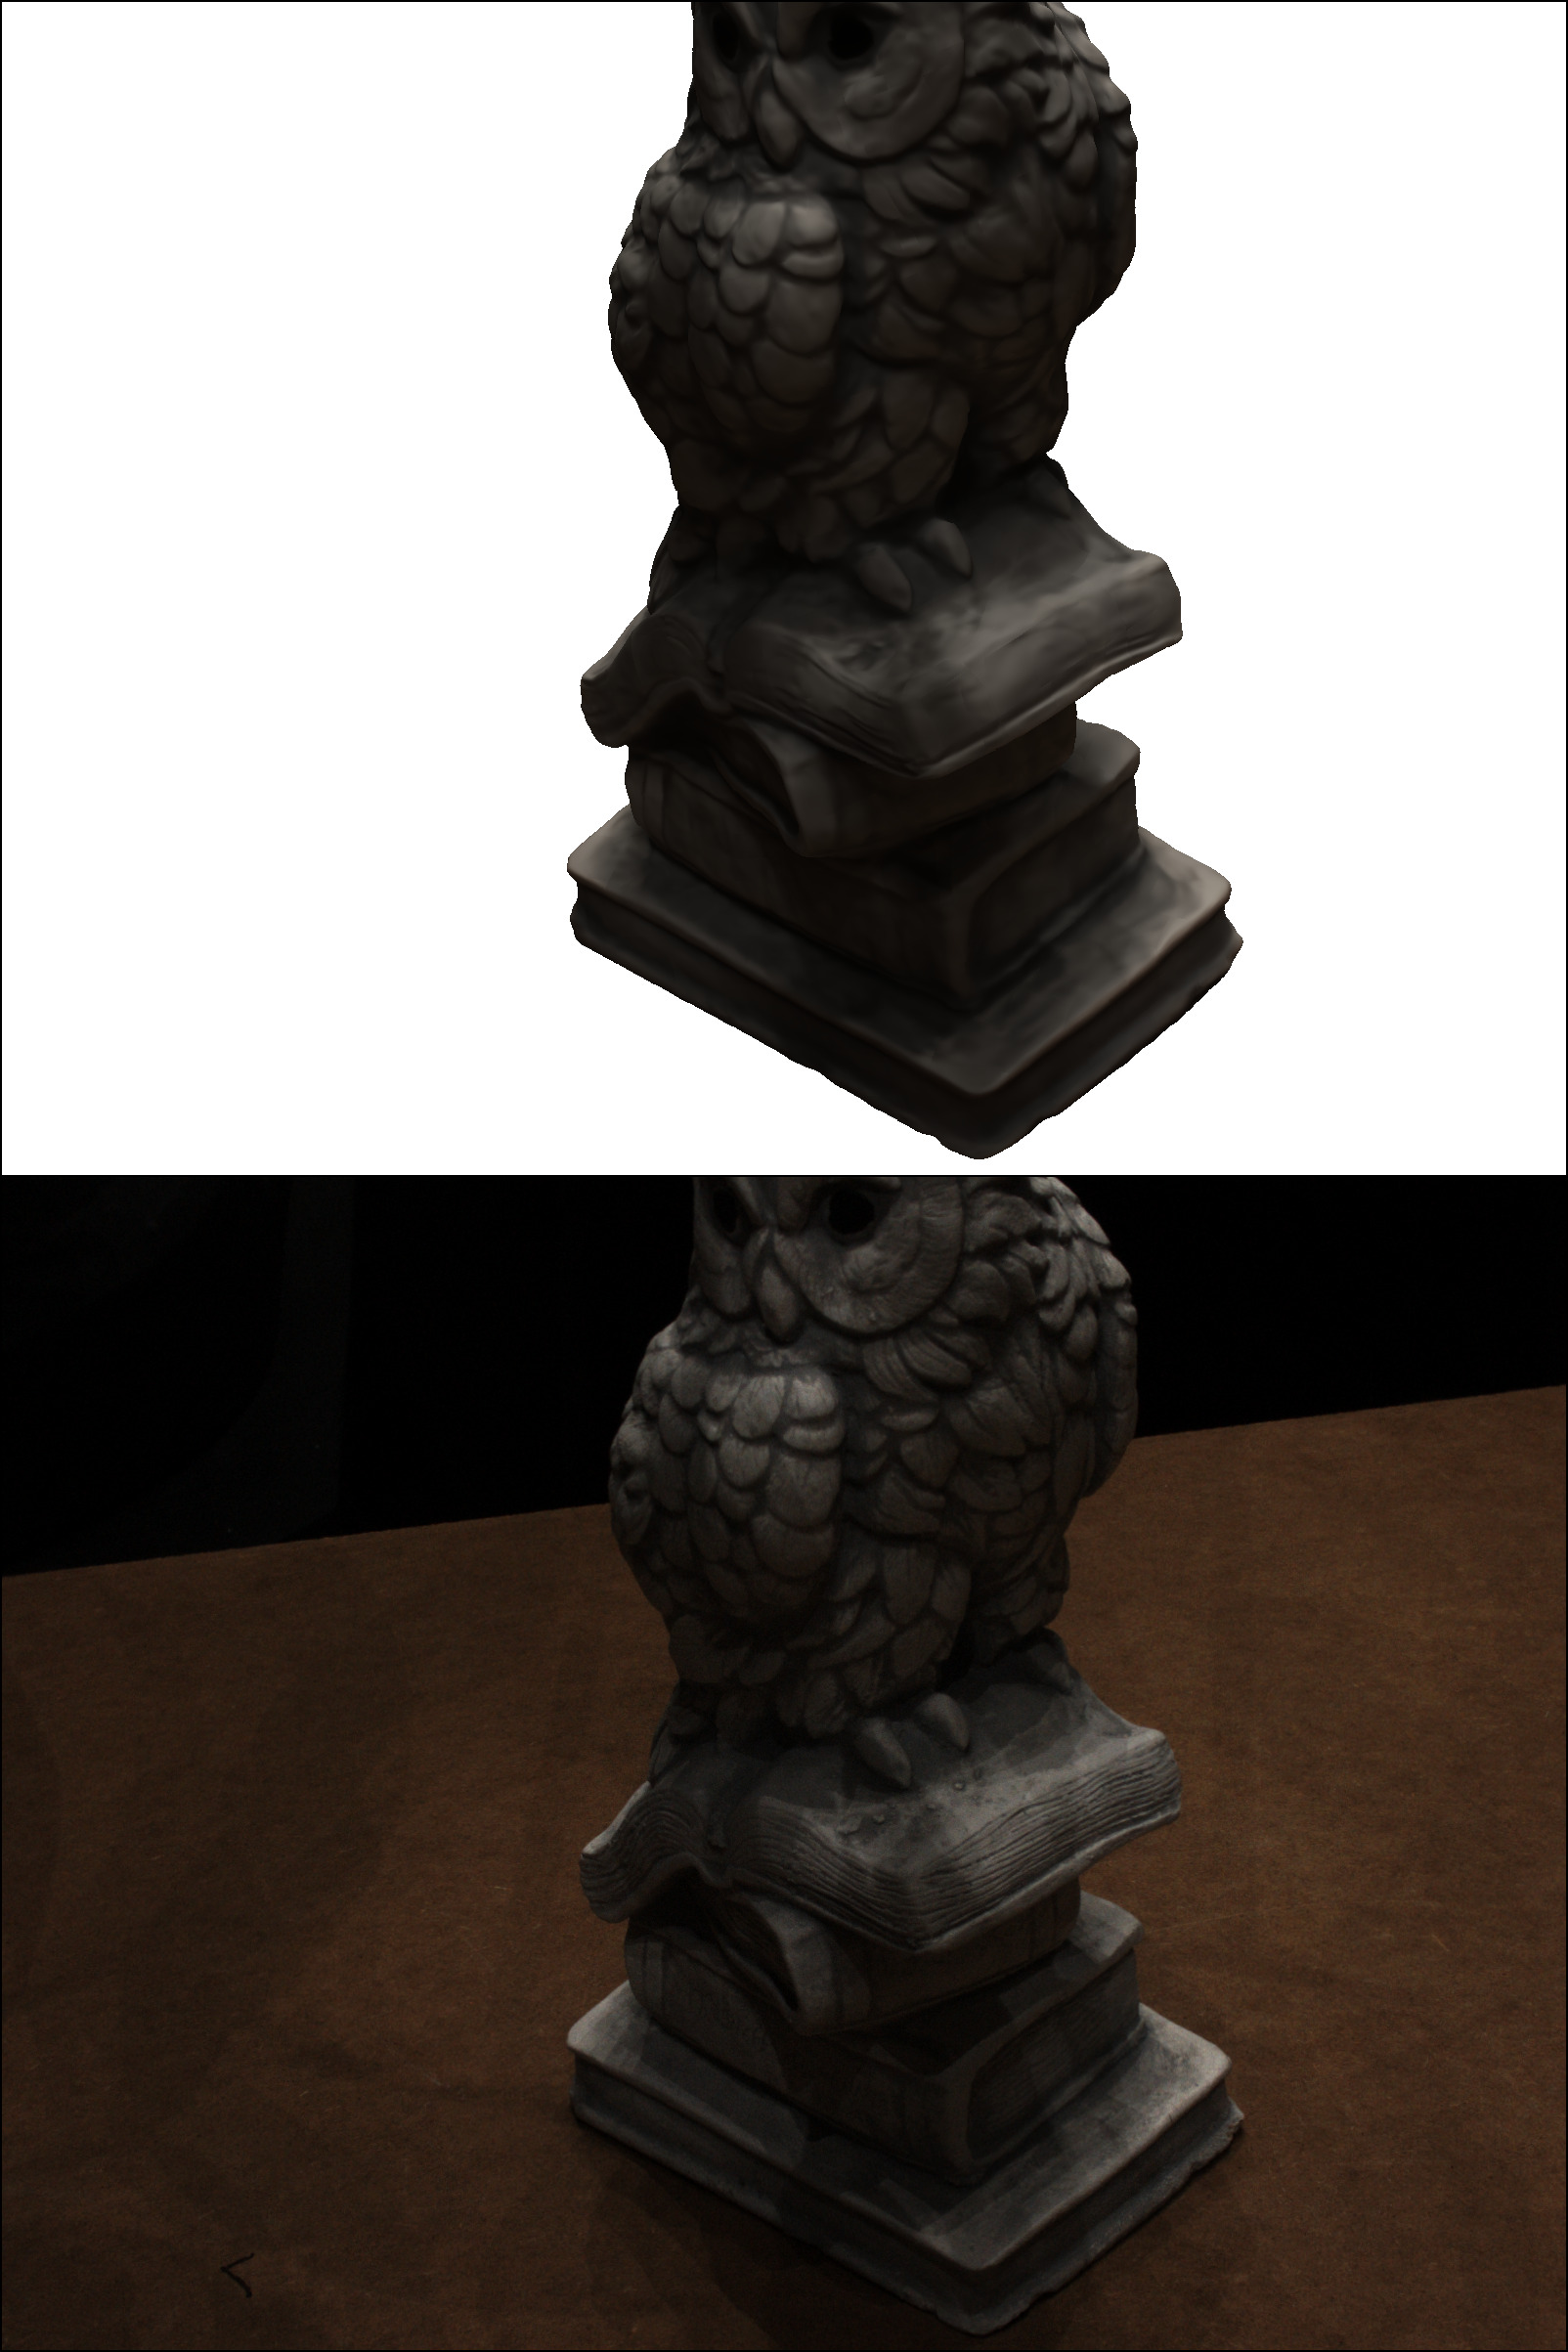
\includegraphics[width=1.5cm]{images/chapter5_img/RenderedImages-DepthMaps-EpochWise-Evals/NFFB/122/rendering_2000.jpg} &  
    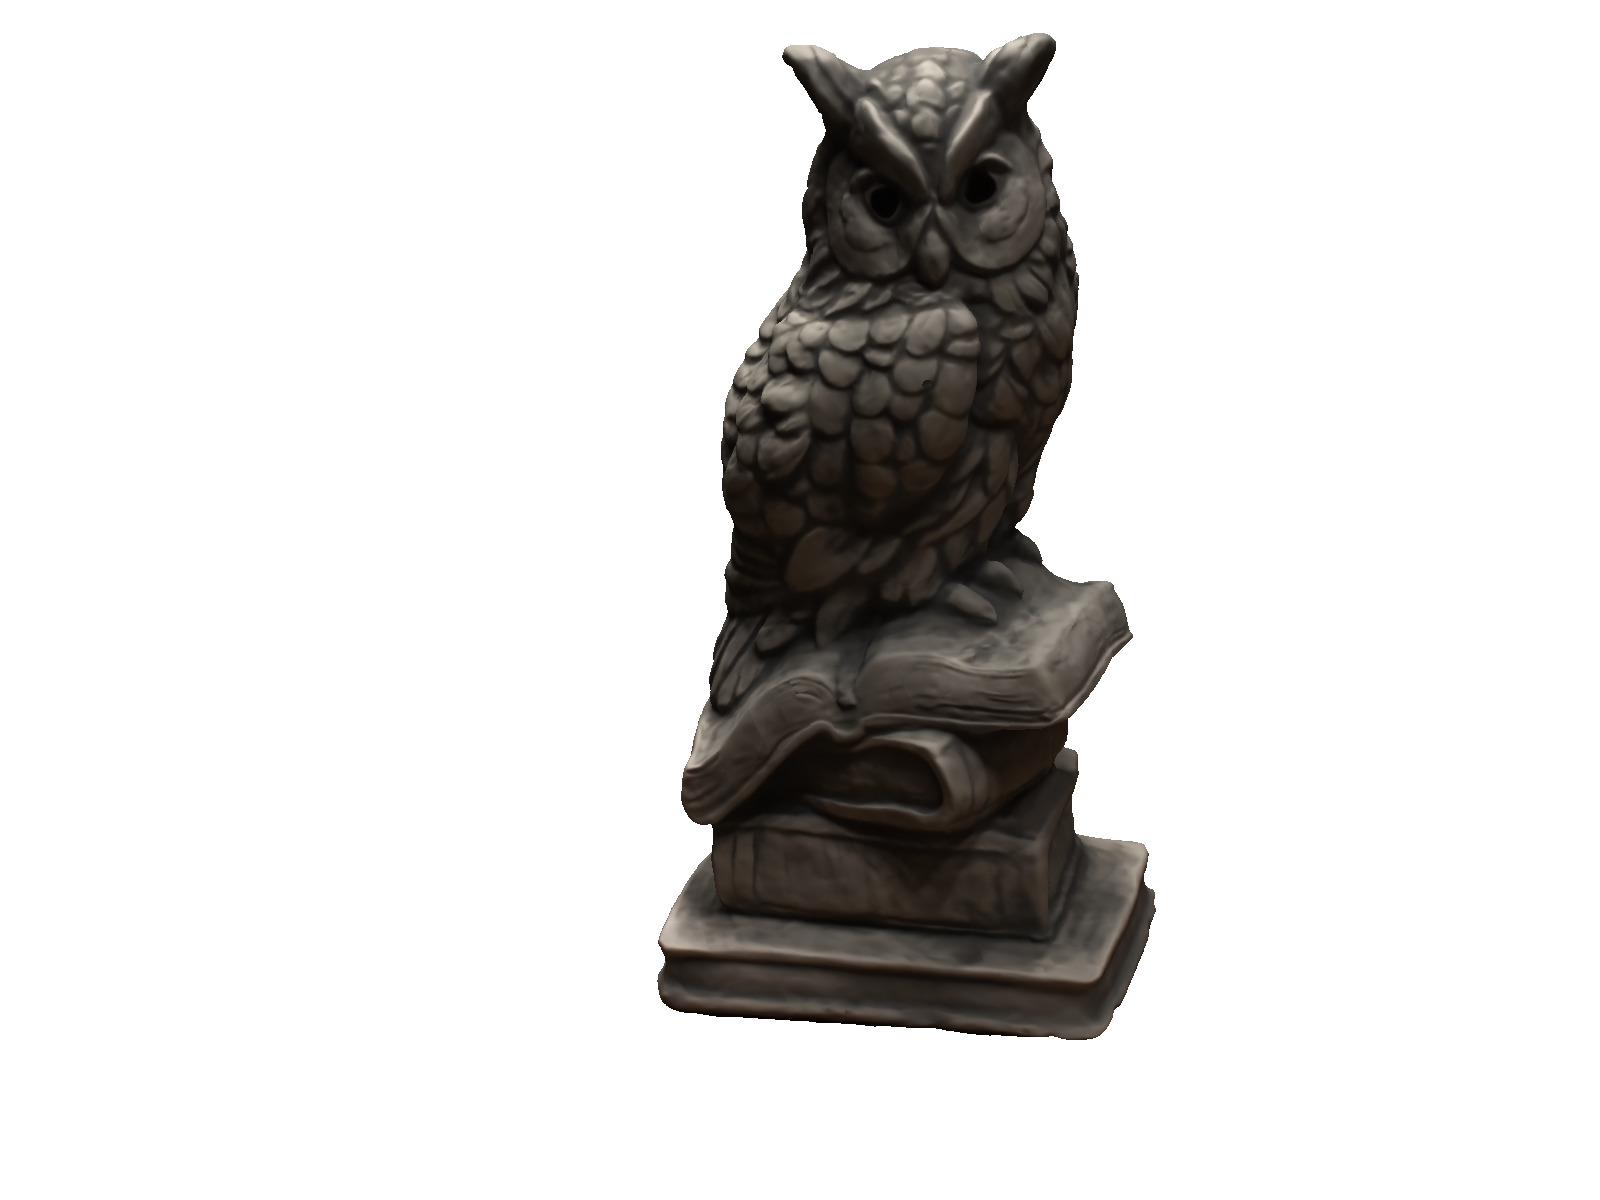
\includegraphics[width=1.5cm]{images/chapter5_img/RenderedImages-DepthMaps-EpochWise-Evals/NFFB/122/eval_055.jpg} \\
    \hline
    StyleMod NFFB & 
    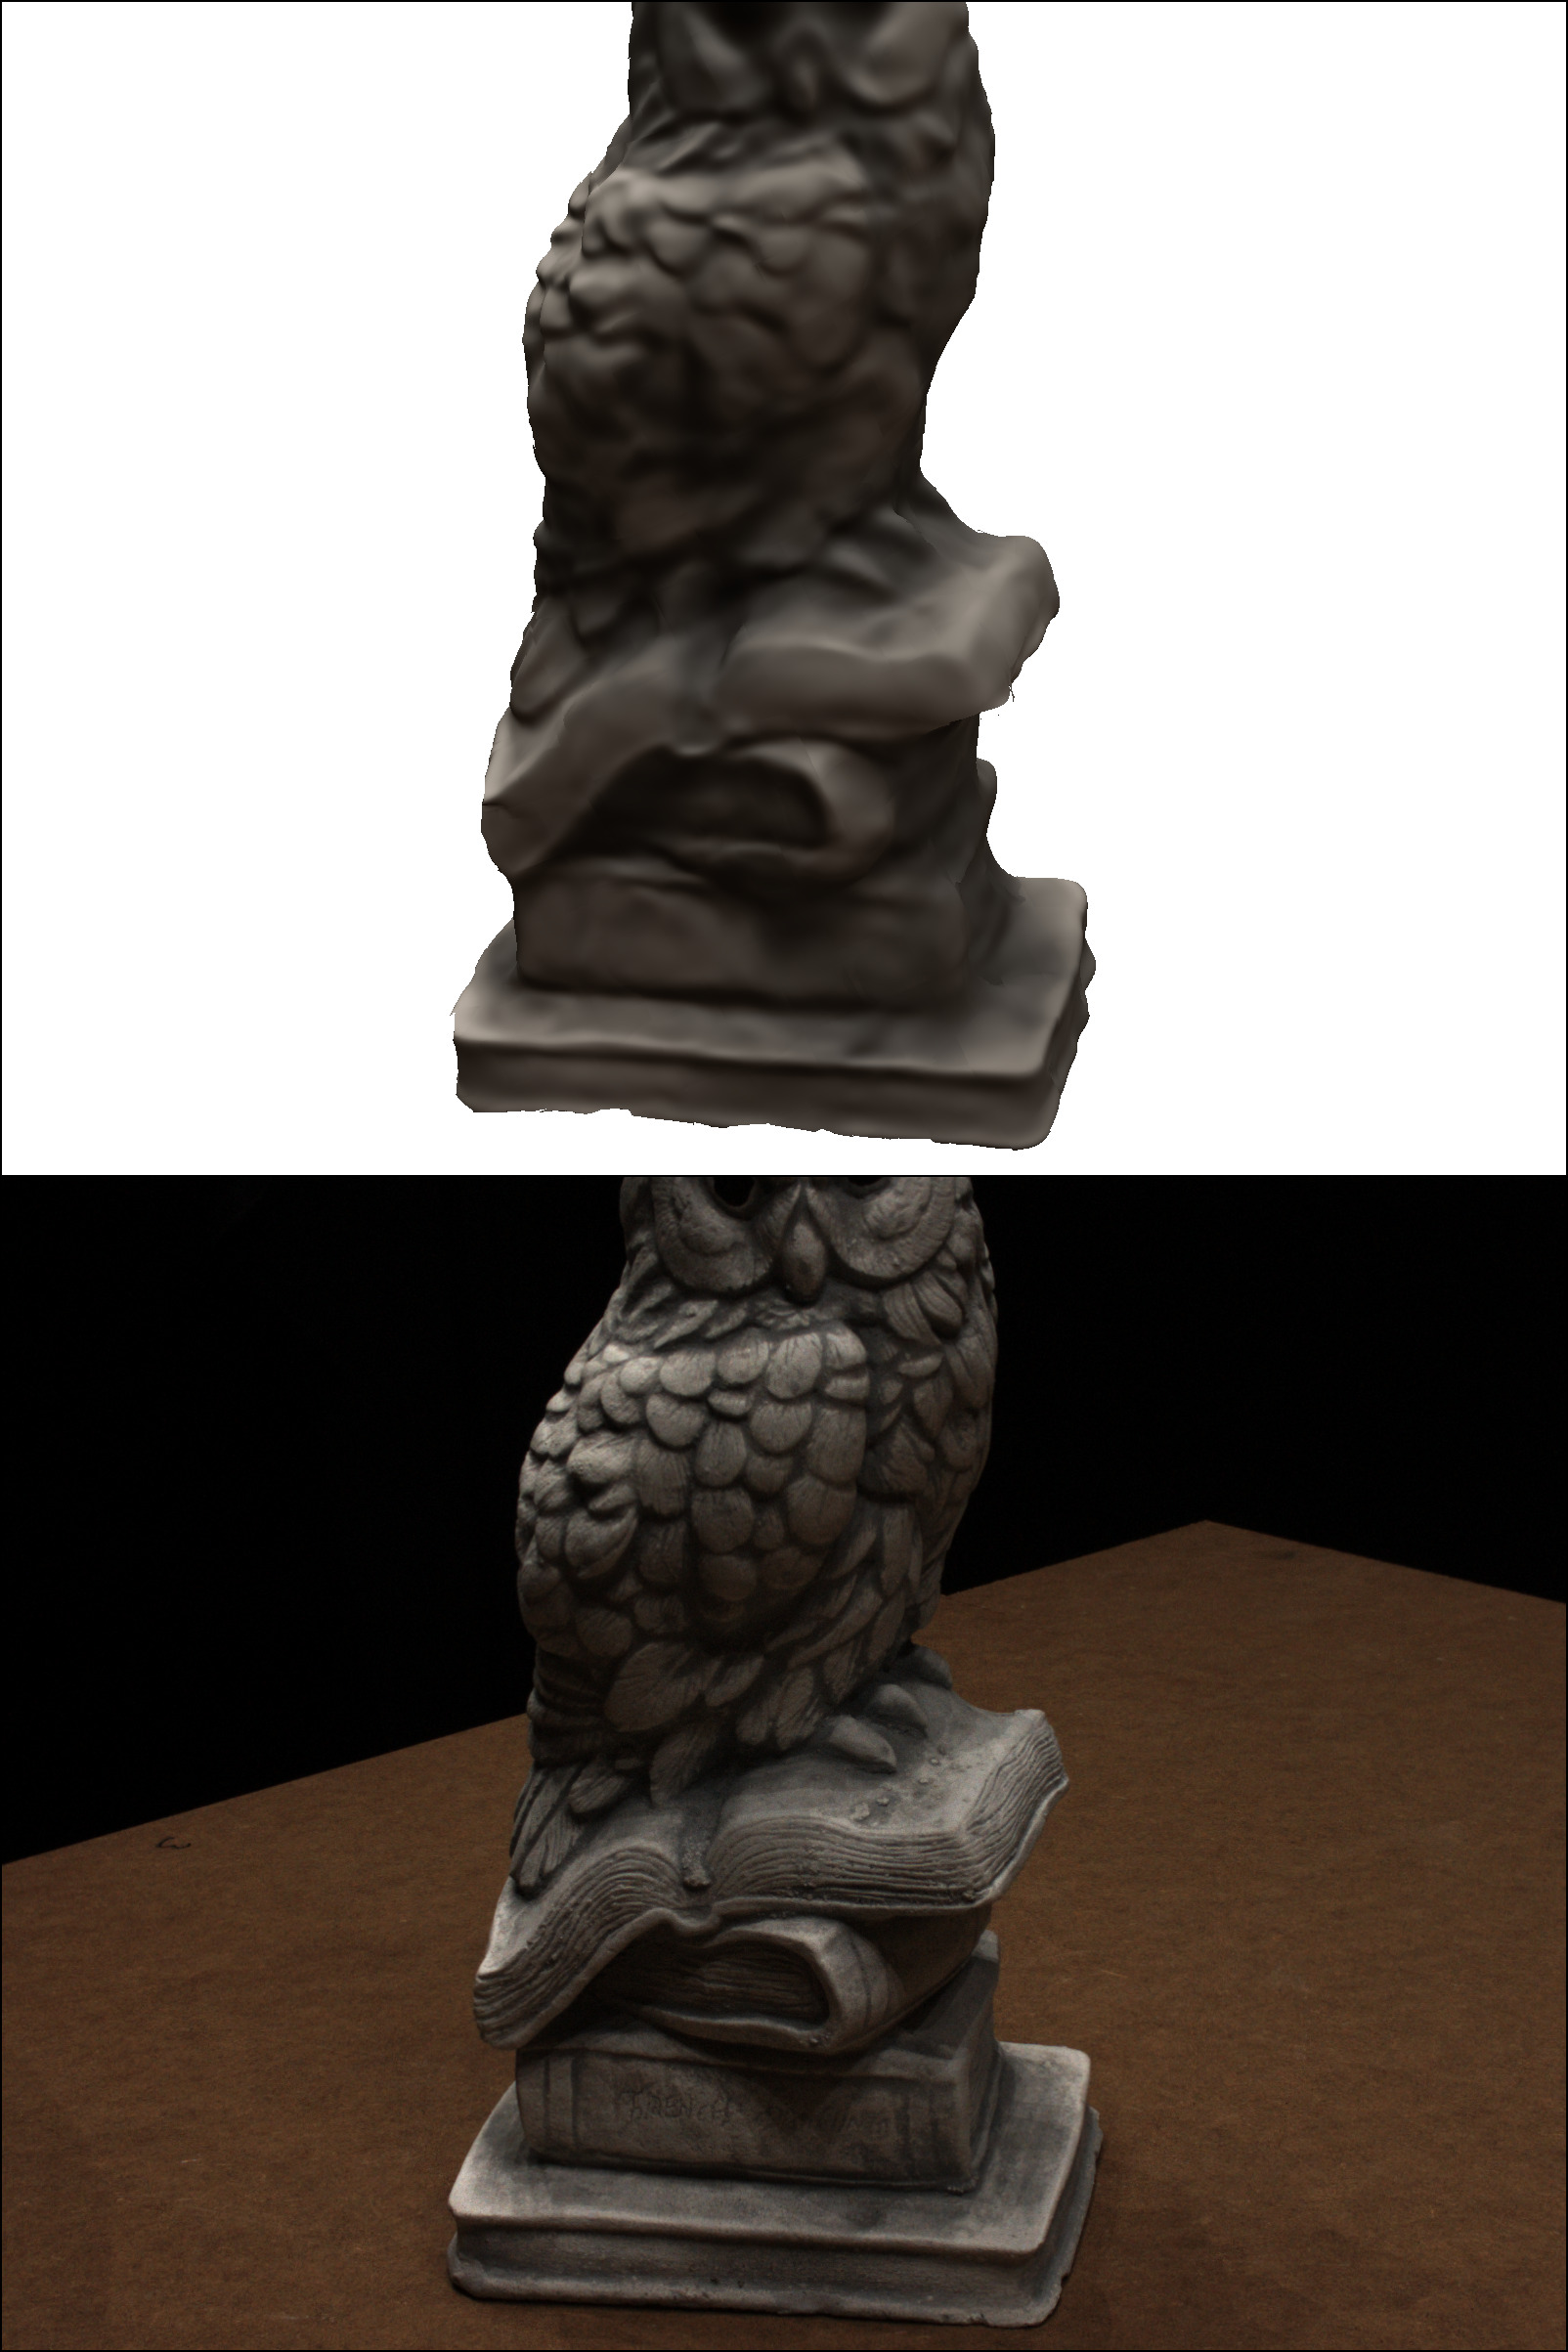
\includegraphics[width=1.5cm]{images/chapter5_img/RenderedImages-DepthMaps-EpochWise-Evals/StylemodNFFB/122/rendering_100.jpg} & 
    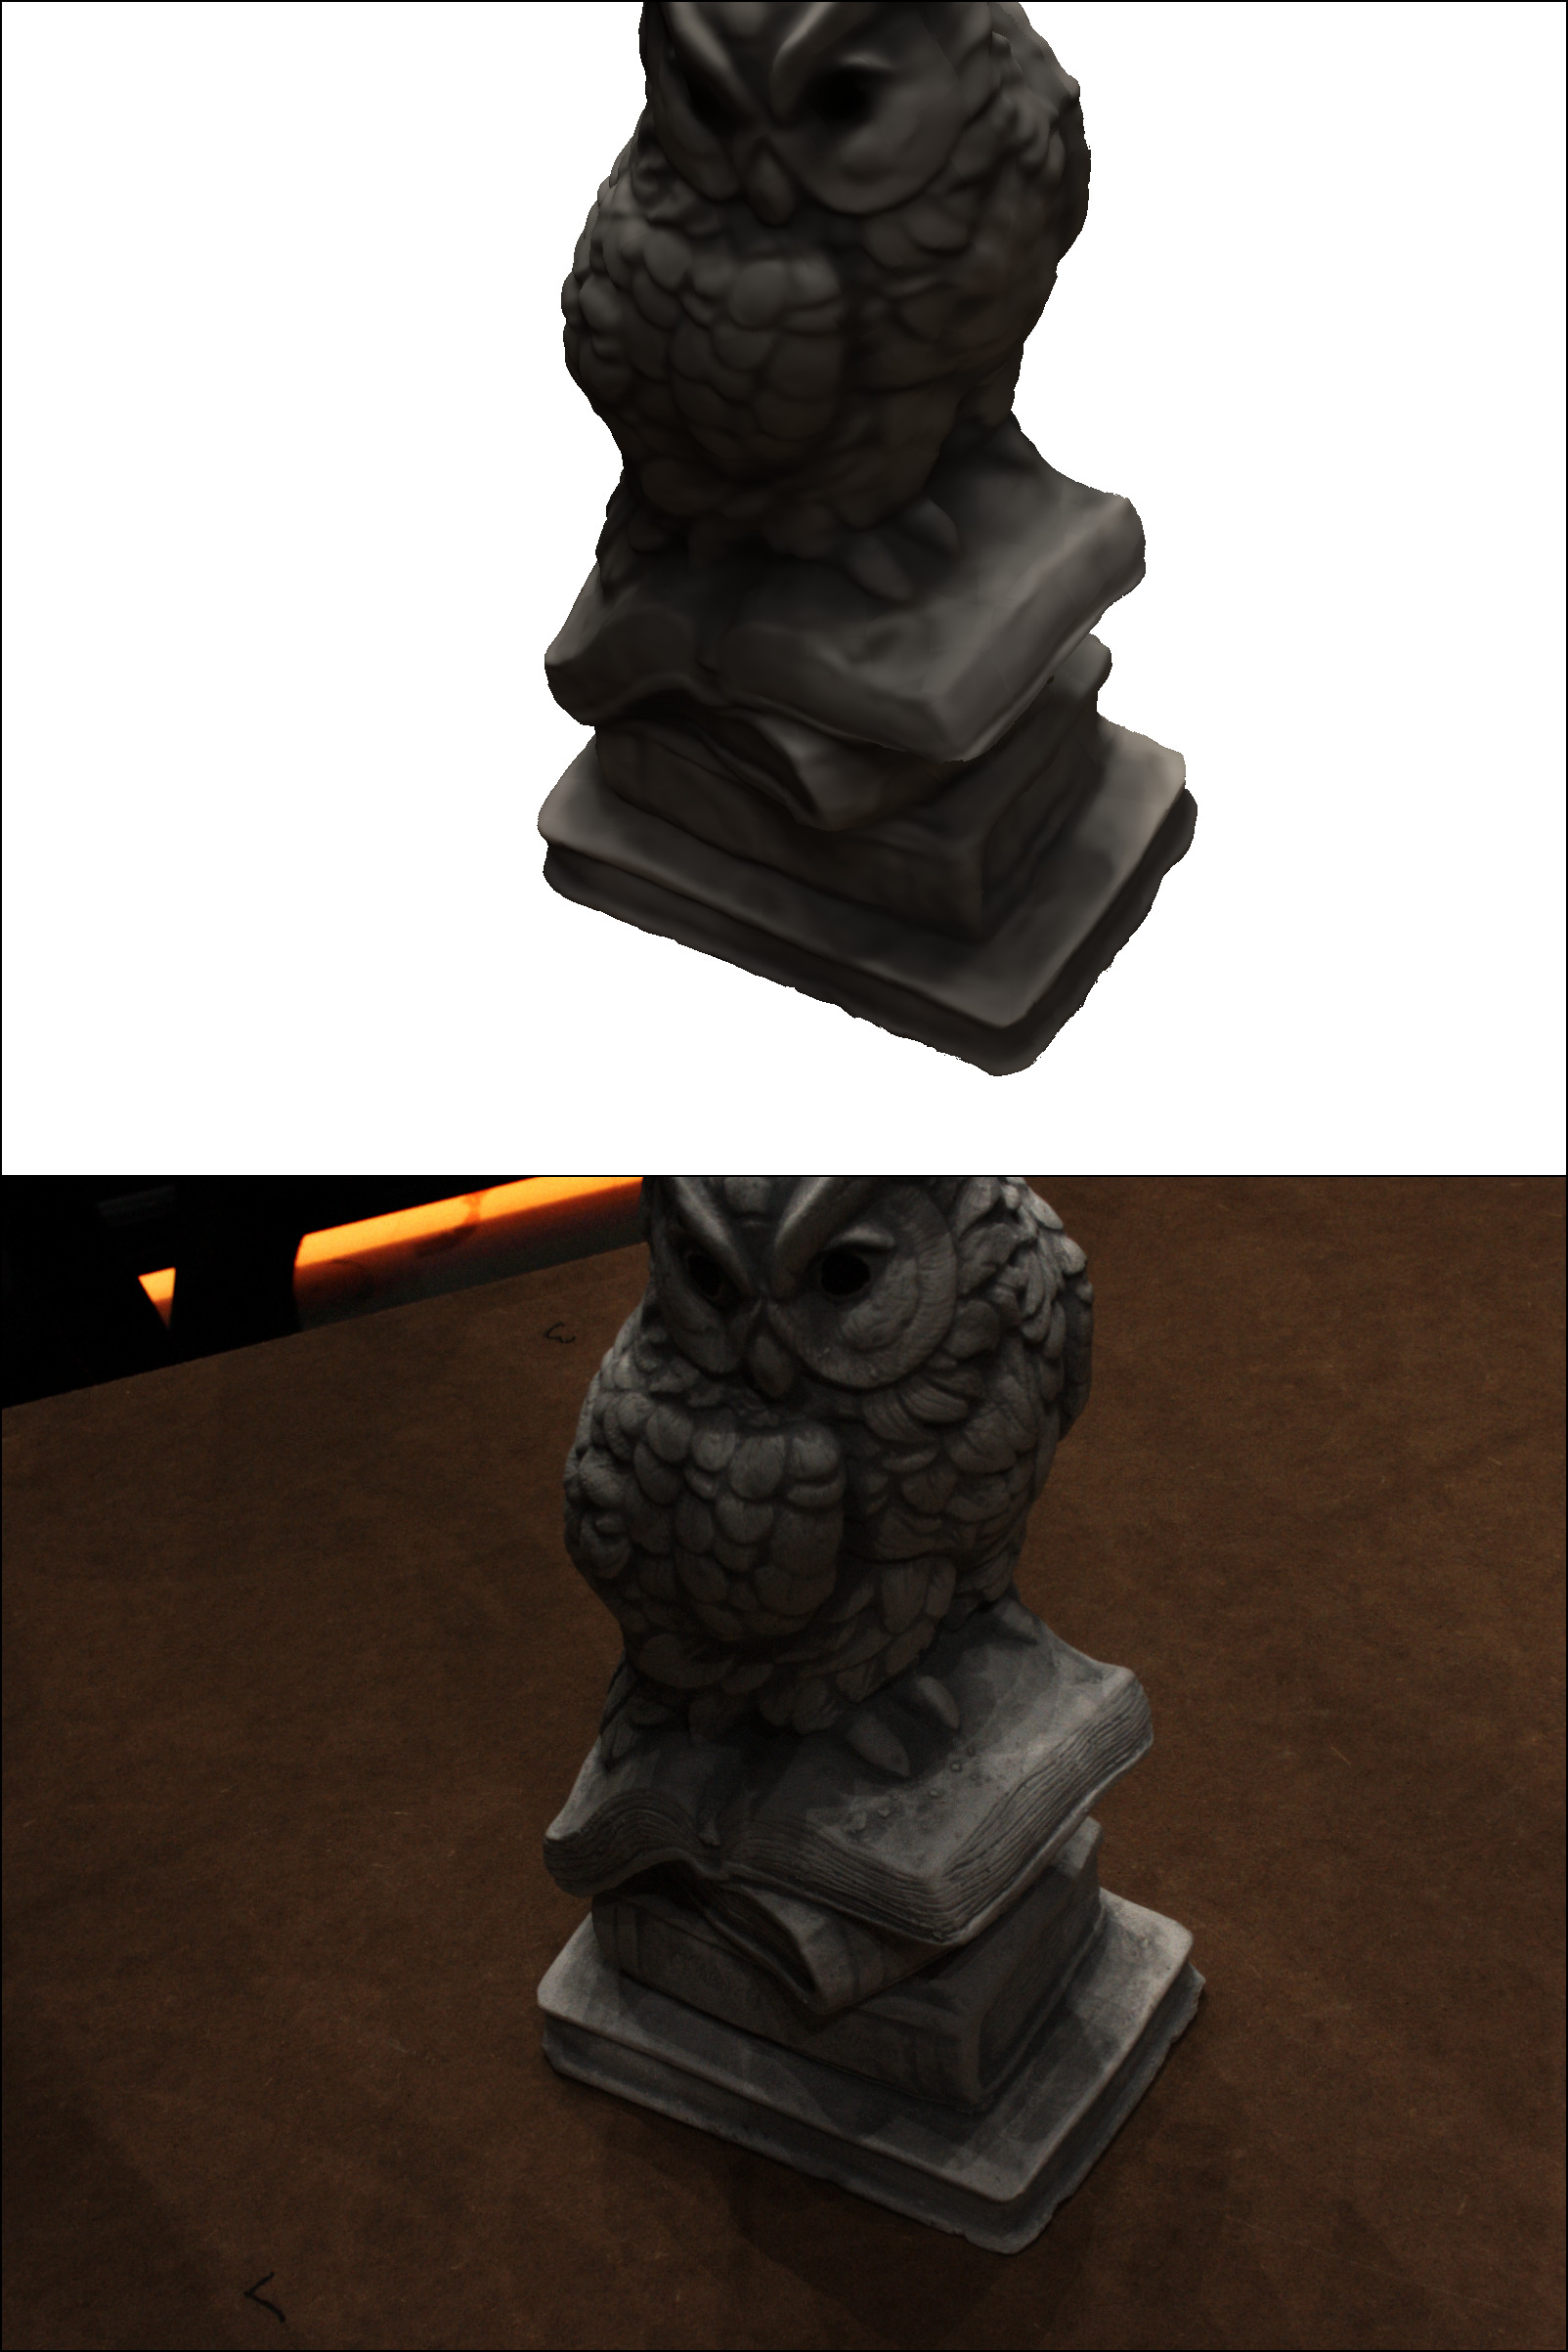
\includegraphics[width=1.5cm]{images/chapter5_img/RenderedImages-DepthMaps-EpochWise-Evals/StylemodNFFB/122/rendering_500.jpg} & 
    \includegraphics[width=1.5cm]{images/chapter5_img/RenderedImages-DepthMaps-EpochWise-Evals/StylemodNFFB/122/rendering_1000.jpg} & 
    \includegraphics[width=1.5cm]{images/chapter5_img/RenderedImages-DepthMaps-EpochWise-Evals/StylemodNFFB/122/rendering_2000.jpg} & 
    \includegraphics[width=1.5cm]{images/chapter5_img/RenderedImages-DepthMaps-EpochWise-Evals/StylemodNFFB/122/eval_055.jpg} \\
    \hline
    StyleModNFFB (TinyCudaNN) & 
     & 
     &
     & 
    \includegraphics[width=1.5cm]{images/chapter5_img/RenderedImages-DepthMaps-EpochWise-Evals/StylemodNFFB_TCNN/122/rendering_2000.jpg} & 
    \includegraphics[width=1.5cm]{images/chapter5_img/RenderedImages-DepthMaps-EpochWise-Evals/StylemodNFFB_TCNN/122/eval_055.jpg} \\
    \hline
    HashGrid3D (TinyCudaNN) & 
     & 
     & 
      & 
    \includegraphics[width=1.5cm]{images/chapter5_img/RenderedImages-DepthMaps-EpochWise-Evals/MRHashGrid3D_TCNN/122/rendering_1500.jpg} & 
    \includegraphics[width=1.5cm]{images/chapter5_img/RenderedImages-DepthMaps-EpochWise-Evals/MRHashGrid3D_TCNN/122/eval_055.jpg} \\
    \hline
    \end{tabular}
    \caption{Αποτελέσματα 3D Ανακατασκευής Σκηνής 122}
\end{table}
\clearpage
\begin{table}[H]
    \centering
    \begin{tabular}{|c|*{6}{p{1.6cm}|}}
    \hline
    Αλγόριθμος & Epoch 100 & Epoch 500 & Epoch 1000 & Epoch 2000 & Eval Πόζα 55 \\
    \hline
    Positional Encoding & 
     &    
     & 
     & 
    \includegraphics[width=1.5cm]{images/chapter5_img/RenderedImages-DepthMaps-EpochWise-Evals/PositionalEncoding/110/rendering_2000.jpg} & 
    \includegraphics[width=1.5cm]{images/chapter5_img/RenderedImages-DepthMaps-EpochWise-Evals/PositionalEncoding/110/eval_055.jpg} \\
    \hline
    FourierNTK & 
    \includegraphics[width=1.5cm]{images/chapter5_img/RenderedImages-DepthMaps-EpochWise-Evals/FourierNTK/110/rendering_100.jpg} & 
    \includegraphics[width=1.5cm]{images/chapter5_img/RenderedImages-DepthMaps-EpochWise-Evals/FourierNTK/110/rendering_500.jpg} & 
    \includegraphics[width=1.5cm]{images/chapter5_img/RenderedImages-DepthMaps-EpochWise-Evals/FourierNTK/110/rendering_1000.jpg} & 
    \includegraphics[width=1.5cm]{images/chapter5_img/RenderedImages-DepthMaps-EpochWise-Evals/FourierNTK/110/rendering_2000.jpg} & 
    \includegraphics[width=1.5cm]{images/chapter5_img/RenderedImages-DepthMaps-EpochWise-Evals/FourierNTK/110/eval_055.jpg} \\
    \hline
    MR-HashGrid3D & 
    \includegraphics[width=1.5cm]{images/chapter5_img/RenderedImages-DepthMaps-EpochWise-Evals/MRHashGrid3D/110/rendering_100.jpg} & 
    \includegraphics[width=1.5cm]{images/chapter5_img/RenderedImages-DepthMaps-EpochWise-Evals/MRHashGrid3D/110/rendering_500.jpg} & 
    \includegraphics[width=1.5cm]{images/chapter5_img/RenderedImages-DepthMaps-EpochWise-Evals/MRHashGrid3D/110/rendering_1000.jpg} & 
    \includegraphics[width=1.5cm]{images/chapter5_img/RenderedImages-DepthMaps-EpochWise-Evals/MRHashGrid3D/110/rendering_2000.jpg} & 
    \includegraphics[width=1.5cm]{images/chapter5_img/RenderedImages-DepthMaps-EpochWise-Evals/MRHashGrid3D/110/eval_055.jpg} \\
    \hline 
    NFFB & 
    \includegraphics[width=1.5cm]{images/chapter5_img/RenderedImages-DepthMaps-EpochWise-Evals/NFFB/110/rendering_100.jpg} & 
    \includegraphics[width=1.5cm]{images/chapter5_img/RenderedImages-DepthMaps-EpochWise-Evals/NFFB/110/rendering_500.jpg} & 
    \includegraphics[width=1.5cm]{images/chapter5_img/RenderedImages-DepthMaps-EpochWise-Evals/NFFB/110/rendering_1000.jpg} & 
    \includegraphics[width=1.5cm]{images/chapter5_img/RenderedImages-DepthMaps-EpochWise-Evals/NFFB/110/rendering_2000.jpg} &  
    \includegraphics[width=1.5cm]{images/chapter5_img/RenderedImages-DepthMaps-EpochWise-Evals/NFFB/110/eval_055.jpg} \\
    \hline
    StyleMod NFFB & 
    \includegraphics[width=1.5cm]{images/chapter5_img/RenderedImages-DepthMaps-EpochWise-Evals/StylemodNFFB/110/rendering_100.jpg} & 
    \includegraphics[width=1.5cm]{images/chapter5_img/RenderedImages-DepthMaps-EpochWise-Evals/StylemodNFFB/110/rendering_500.jpg} & 
    \includegraphics[width=1.5cm]{images/chapter5_img/RenderedImages-DepthMaps-EpochWise-Evals/StylemodNFFB/110/rendering_1000.jpg} & 
    \includegraphics[width=1.5cm]{images/chapter5_img/RenderedImages-DepthMaps-EpochWise-Evals/StylemodNFFB/110/rendering_2000.jpg} & 
    \includegraphics[width=1.5cm]{images/chapter5_img/RenderedImages-DepthMaps-EpochWise-Evals/StylemodNFFB/110/eval_055.jpg} \\
    \hline
    StyleModNFFB (TinyCudaNN) & 
    \includegraphics[width=1.5cm]{images/chapter5_img/RenderedImages-DepthMaps-EpochWise-Evals/StylemodNFFB_TCNN/110/rendering_100.jpg} & 
    \includegraphics[width=1.5cm]{images/chapter5_img/RenderedImages-DepthMaps-EpochWise-Evals/StylemodNFFB_TCNN/110/rendering_500.jpg} & 
    \includegraphics[width=1.5cm]{images/chapter5_img/RenderedImages-DepthMaps-EpochWise-Evals/StylemodNFFB_TCNN/110/rendering_1000.jpg} & 
    \includegraphics[width=1.5cm]{images/chapter5_img/RenderedImages-DepthMaps-EpochWise-Evals/StylemodNFFB_TCNN/110/rendering_2000.jpg} & 
    \includegraphics[width=1.5cm]{images/chapter5_img/RenderedImages-DepthMaps-EpochWise-Evals/StylemodNFFB_TCNN/110/eval_055.jpg} \\
    \hline
    HashGrid3D (TinyCudaNN) & 
     & 
     & 
     & 
    \includegraphics[width=1.5cm]{images/chapter5_img/RenderedImages-DepthMaps-EpochWise-Evals/MRHashGrid3D_TCNN/110/rendering_2000.jpg} & 
    \includegraphics[width=1.5cm]{images/chapter5_img/RenderedImages-DepthMaps-EpochWise-Evals/MRHashGrid3D_TCNN/110/eval_055.jpg} \\
    \hline
    \end{tabular}
\caption{Αποτελέσματα 3D Ανακατασκευής Σκηνής 110}
\end{table}
\clearpage
\begin{table}[H]
    \centering
    \begin{tabular}{|c|*{6}{p{1.6cm}|}}
    \hline
    Αλγόριθμος & Epoch 100 & Epoch 500 & Epoch 1000 & Epoch 2000 & Eval Πόζα 55 \\
    \hline
    Positional Encoding & 
     &    
    & 
    & 
    \includegraphics[width=1.5cm]{images/chapter5_img/RenderedImages-DepthMaps-EpochWise-Evals/PositionalEncoding/114/rendering_2000.jpg} & 
    \includegraphics[width=1.5cm]{images/chapter5_img/RenderedImages-DepthMaps-EpochWise-Evals/PositionalEncoding/114/eval_055.jpg} \\
    \hline
    FourierNTK & 
    \includegraphics[width=1.5cm]{images/chapter5_img/RenderedImages-DepthMaps-EpochWise-Evals/FourierNTK/114/rendering_100.jpg} & 
    \includegraphics[width=1.5cm]{images/chapter5_img/RenderedImages-DepthMaps-EpochWise-Evals/FourierNTK/114/rendering_500.jpg} & 
    \includegraphics[width=1.5cm]{images/chapter5_img/RenderedImages-DepthMaps-EpochWise-Evals/FourierNTK/114/rendering_1000.jpg} & 
    \includegraphics[width=1.5cm]{images/chapter5_img/RenderedImages-DepthMaps-EpochWise-Evals/FourierNTK/114/rendering_2000.jpg} & 
    \includegraphics[width=1.5cm]{images/chapter5_img/RenderedImages-DepthMaps-EpochWise-Evals/FourierNTK/114/eval_055.jpg} \\
    \hline
    MR-HashGrid3D & 
    & 
    & 
    & 
    \includegraphics[width=1.5cm]{images/chapter5_img/RenderedImages-DepthMaps-EpochWise-Evals/MRHashGrid3D/114/rendering_2000.jpg} & 
    \includegraphics[width=1.5cm]{images/chapter5_img/RenderedImages-DepthMaps-EpochWise-Evals/MRHashGrid3D/114/eval_055.jpg} \\
    \hline 
    NFFB & 
    \includegraphics[width=1.5cm]{images/chapter5_img/RenderedImages-DepthMaps-EpochWise-Evals/NFFB/114/rendering_100.jpg} & 
    \includegraphics[width=1.5cm]{images/chapter5_img/RenderedImages-DepthMaps-EpochWise-Evals/NFFB/114/rendering_500.jpg} & 
    \includegraphics[width=1.5cm]{images/chapter5_img/RenderedImages-DepthMaps-EpochWise-Evals/NFFB/114/rendering_1000.jpg} & 
    \includegraphics[width=1.5cm]{images/chapter5_img/RenderedImages-DepthMaps-EpochWise-Evals/NFFB/114/rendering_2000.jpg} &  
    \includegraphics[width=1.5cm]{images/chapter5_img/RenderedImages-DepthMaps-EpochWise-Evals/NFFB/114/eval_055.jpg} \\
    \hline
    StyleMod NFFB & 
    \includegraphics[width=1.5cm]{images/chapter5_img/RenderedImages-DepthMaps-EpochWise-Evals/StylemodNFFB/114/rendering_100.jpg} & 
    \includegraphics[width=1.5cm]{images/chapter5_img/RenderedImages-DepthMaps-EpochWise-Evals/StylemodNFFB/114/rendering_500.jpg} & 
    \includegraphics[width=1.5cm]{images/chapter5_img/RenderedImages-DepthMaps-EpochWise-Evals/StylemodNFFB/114/rendering_1000.jpg} & 
    \includegraphics[width=1.5cm]{images/chapter5_img/RenderedImages-DepthMaps-EpochWise-Evals/StylemodNFFB/114/rendering_2000.jpg} & 
    \includegraphics[width=1.5cm]{images/chapter5_img/RenderedImages-DepthMaps-EpochWise-Evals/StylemodNFFB/114/eval_055.jpg} \\
    \hline
    StyleModNFFB (TinyCudaNN) & 
    \includegraphics[width=1.5cm]{images/chapter5_img/RenderedImages-DepthMaps-EpochWise-Evals/StylemodNFFB_TCNN/114/rendering_100.jpg} & 
    \includegraphics[width=1.5cm]{images/chapter5_img/RenderedImages-DepthMaps-EpochWise-Evals/StylemodNFFB_TCNN/114/rendering_500.jpg} & 
    \includegraphics[width=1.5cm]{images/chapter5_img/RenderedImages-DepthMaps-EpochWise-Evals/StylemodNFFB_TCNN/114/rendering_1000.jpg} & 
    \includegraphics[width=1.5cm]{images/chapter5_img/RenderedImages-DepthMaps-EpochWise-Evals/StylemodNFFB_TCNN/114/rendering_2000.jpg} & 
    \includegraphics[width=1.5cm]{images/chapter5_img/RenderedImages-DepthMaps-EpochWise-Evals/StylemodNFFB_TCNN/114/eval_055.jpg} \\
    \hline
    \end{tabular}
\caption{Αποτελέσματα 3D Ανακατασκευής Σκηνής 114}
\end{table}


\par
   Παρατηρώντας τα αποτελέσματα, βλέπουμε ότι τα μοντέλα \enit{SylemodNFFB}, \enit{NFFB}, και οι αντίστοιχες συγχωνευμένες μορφές τους όσον αφορά την κωδικοποίηση \enit{HashGrid TCNN} συγκλίνουν πολύ πιο γρήγορα στις επιθυμητές παραμέτρους εμφάνισης (χρειάζονται μόνο 500 εποχές) και μάλιστα κάποια από αυτά, είναι σε θέση να αποδώσουν στοιχεία φωτισμού που αντιστοιχούν στο υλικό/υφή  (\enit{Phong Material}). Το κλασσικό \enit{IDR}, προσπαθεί να πετύχει αποτελέσματα αυτής της μορφής, αλλά δεν τα καταφέρνει για όλα τα μοντέλα αφού δεν εκπαιδεύεται για τέτοια χαρακτηριστικά του πεδίου φωτισμού. Παρ' όλα αυτά, σε κάποιες εικόνες μπορεί να δούμε λανθασμένα τεχνουργήματα (\enit{artifacts}) του δικτύου. Πόρισμα είναι ότι έχουν να κάνουν με την σφάλμα μάσκας το οποίο δεν διαδίδεται με σωστές αριθμητικές τιμές στο δίκτυο γεωμετρίας. 
\par
    Οι εικόνες που λείπουν είναι σε εποχές που διακόπηκε η εκπαίδευση ή δεν εκτύπωσαν το αποτέλεσμα(πειράματα υπολογιστικής συστοιχίας) λόγω επανεκκίνησης της εκπαίδευσης. \footnote{Η διακοπή της εκπαίδευσης, μπορεί να συμβεί λόγω υπέρβασης των ορίων μνήμης ή κάποιας άλλης διακοπής. Ωστόσο, αποθηκεύεται μοντέλο σε τακτά χρονικά διαστήματα .}


\subsection{Αποτύπωσης Προσέγγισης Δυαδικής μάσκας - Μάσκα <<βάθους>> ανά εποχή}
\begin{table}[H]
    \centering
    \begin{tabular}{|c|*{5}{p{1.6cm}|}}
    \hline
    Αλγόριθμος & Εποχή 100 & Εποχή 500 & Εποχή 1000 & Εποχή 2000\\
    \hline
    Positional Encoding & 
    \includegraphics[width=1.5cm]{images/chapter5_img/RenderedImages-DepthMaps-EpochWise-Evals/PositionalEncoding/65/depth_100.jpg} & 
    \includegraphics[width=1.5cm]{images/chapter5_img/RenderedImages-DepthMaps-EpochWise-Evals/PositionalEncoding/65/depth_500.jpg} & 
    \includegraphics[width=1.5cm]{images/chapter5_img/RenderedImages-DepthMaps-EpochWise-Evals/PositionalEncoding/65/depth_1000.jpg} & 
    \includegraphics[width=1.5cm]{images/chapter5_img/RenderedImages-DepthMaps-EpochWise-Evals/PositionalEncoding/65/depth_2000.jpg} \\
    \hline
    FourierNTK & 
    \includegraphics[width=1.5cm]{images/chapter5_img/RenderedImages-DepthMaps-EpochWise-Evals/FourierNTK/65/depth_100.jpg} & 
    \includegraphics[width=1.5cm]{images/chapter5_img/RenderedImages-DepthMaps-EpochWise-Evals/FourierNTK/65/depth_500.jpg} & 
    \includegraphics[width=1.5cm]{images/chapter5_img/RenderedImages-DepthMaps-EpochWise-Evals/FourierNTK/65/depth_1000.jpg} & 
    \includegraphics[width=1.5cm]{images/chapter5_img/RenderedImages-DepthMaps-EpochWise-Evals/FourierNTK/65/depth_2000.jpg}\\
    \hline
    MR-HashGrid3D & 
    \includegraphics[width=1.5cm]{images/chapter5_img/RenderedImages-DepthMaps-EpochWise-Evals/MRHashGrid3D/65/depth_100.jpg} & 
    \includegraphics[width=1.5cm]{images/chapter5_img/RenderedImages-DepthMaps-EpochWise-Evals/MRHashGrid3D/65/depth_500.jpg} & 
    \includegraphics[width=1.5cm]{images/chapter5_img/RenderedImages-DepthMaps-EpochWise-Evals/MRHashGrid3D/65/depth_1000.jpg} & 
    \includegraphics[width=1.5cm]{images/chapter5_img/RenderedImages-DepthMaps-EpochWise-Evals/MRHashGrid3D/65/depth_2000.jpg} \\
    \hline 
    NFFB & 
    \includegraphics[width=1.5cm]{images/chapter5_img/RenderedImages-DepthMaps-EpochWise-Evals/NFFB/65/depth_100.jpg} & 
    \includegraphics[width=1.5cm]{images/chapter5_img/RenderedImages-DepthMaps-EpochWise-Evals/NFFB/65/depth_500.jpg} & 
    \includegraphics[width=1.5cm]{images/chapter5_img/RenderedImages-DepthMaps-EpochWise-Evals/NFFB/65/depth_1000.jpg} & 
    \includegraphics[width=1.5cm]{images/chapter5_img/RenderedImages-DepthMaps-EpochWise-Evals/NFFB/65/depth_2000.jpg}  \\
    \hline
    StyleMod NFFB & 
    \includegraphics[width=1.5cm]{images/chapter5_img/RenderedImages-DepthMaps-EpochWise-Evals/StylemodNFFB/65/depth_100.jpg} & 
    \includegraphics[width=1.5cm]{images/chapter5_img/RenderedImages-DepthMaps-EpochWise-Evals/StylemodNFFB/65/depth_500.jpg} & 
    \includegraphics[width=1.5cm]{images/chapter5_img/RenderedImages-DepthMaps-EpochWise-Evals/StylemodNFFB/65/depth_1000.jpg} & 
    \includegraphics[width=1.5cm]{images/chapter5_img/RenderedImages-DepthMaps-EpochWise-Evals/StylemodNFFB/65/depth_2000.jpg} \\ 
    \hline
    StyleModNFFB (TinyCudaNN) & 
    \includegraphics[width=1.5cm]{images/chapter5_img/RenderedImages-DepthMaps-EpochWise-Evals/StylemodNFFB_TCNN/65/depth_100.jpg} & 
    \includegraphics[width=1.5cm]{images/chapter5_img/RenderedImages-DepthMaps-EpochWise-Evals/StylemodNFFB_TCNN/65/depth_500.jpg} & 
    \includegraphics[width=1.5cm]{images/chapter5_img/RenderedImages-DepthMaps-EpochWise-Evals/StylemodNFFB_TCNN/65/depth_1000.jpg} & 
    \includegraphics[width=1.5cm]{images/chapter5_img/RenderedImages-DepthMaps-EpochWise-Evals/StylemodNFFB_TCNN/65/depth_2000.jpg} \\
    \hline
    
    \end{tabular}
    \caption{Αποτελέσματα 3D Ανακατασκευής Σκηνής 65 - Μάσκα Βάθους}
    \end{table}


    \begin{table}[H]
    \centering
    \begin{tabular}{|c|*{5}{p{1.6cm}|}}
    \hline
    Αλγόριθμος & Εποχή 100 & Εποχή 500 & Εποχή 1000 & Εποχή 2000\\
    \hline
    Positional Encoding & 
     & 
     & 
     & 
    \includegraphics[width=1.5cm]{images/chapter5_img/RenderedImages-DepthMaps-EpochWise-Evals/PositionalEncoding/122/depth_2000.jpg} \\
    \hline
    FourierNTK & 
    \includegraphics[width=1.5cm]{images/chapter5_img/RenderedImages-DepthMaps-EpochWise-Evals/FourierNTK/122/depth_100.jpg} & 
    \includegraphics[width=1.5cm]{images/chapter5_img/RenderedImages-DepthMaps-EpochWise-Evals/FourierNTK/122/depth_500.jpg} & 
    \includegraphics[width=1.5cm]{images/chapter5_img/RenderedImages-DepthMaps-EpochWise-Evals/FourierNTK/122/depth_1000.jpg} & 
    \includegraphics[width=1.5cm]{images/chapter5_img/RenderedImages-DepthMaps-EpochWise-Evals/FourierNTK/122/depth_2000.jpg}\\
    \hline
    MR-HashGrid3D & 
    \includegraphics[width=1.5cm]{images/chapter5_img/RenderedImages-DepthMaps-EpochWise-Evals/MRHashGrid3D/122/depth_100.jpg} & 
    \includegraphics[width=1.5cm]{images/chapter5_img/RenderedImages-DepthMaps-EpochWise-Evals/MRHashGrid3D/122/depth_500.jpg} & 
    \includegraphics[width=1.5cm]{images/chapter5_img/RenderedImages-DepthMaps-EpochWise-Evals/MRHashGrid3D/122/depth_1000.jpg} & 
    \includegraphics[width=1.5cm]{images/chapter5_img/RenderedImages-DepthMaps-EpochWise-Evals/MRHashGrid3D/122/depth_2000.jpg} \\
    \hline 
    NFFB & 
    \includegraphics[width=1.5cm]{images/chapter5_img/RenderedImages-DepthMaps-EpochWise-Evals/NFFB/122/depth_100.jpg} & 
    \includegraphics[width=1.5cm]{images/chapter5_img/RenderedImages-DepthMaps-EpochWise-Evals/NFFB/122/depth_500.jpg} & 
    \includegraphics[width=1.5cm]{images/chapter5_img/RenderedImages-DepthMaps-EpochWise-Evals/NFFB/122/depth_1000.jpg} &   \\
    \hline
    StyleMod NFFB & 
    \includegraphics[width=1.5cm]{images/chapter5_img/RenderedImages-DepthMaps-EpochWise-Evals/StylemodNFFB/122/depth_100.jpg} & 
    \includegraphics[width=1.5cm]{images/chapter5_img/RenderedImages-DepthMaps-EpochWise-Evals/StylemodNFFB/122/depth_500.jpg} & 
    \includegraphics[width=1.5cm]{images/chapter5_img/RenderedImages-DepthMaps-EpochWise-Evals/StylemodNFFB/122/depth_1000.jpg} & 
    \includegraphics[width=1.5cm]{images/chapter5_img/RenderedImages-DepthMaps-EpochWise-Evals/StylemodNFFB/122/depth_2000.jpg} \\ 
    \hline
    StyleModNFFB (TinyCudaNN) & 
     & 
     & 
     & 
    \includegraphics[width=1.5cm]{images/chapter5_img/RenderedImages-DepthMaps-EpochWise-Evals/StylemodNFFB_TCNN/122/depth_2000.jpg} \\
    \hline
    
    \end{tabular}
    \caption{Αποτελέσματα 3D Ανακατασκευής Σκηνής 122 - Μάσκα Βάθους}
    \end{table}


    
    \begin{table}[H]
    \centering
    \begin{tabular}{|c|*{5}{p{1.6cm}|}}
    \hline
    Αλγόριθμος & Εποχή 100 & Εποχή 500 & Εποχή 1000 & Εποχή 2000\\
    \hline
    Positional Encoding & 
    & 
    & 
    & 
    \includegraphics[width=1.5cm]{images/chapter5_img/RenderedImages-DepthMaps-EpochWise-Evals/PositionalEncoding/110/depth_2000.jpg} \\
    \hline
    FourierNTK & 
    \includegraphics[width=1.5cm]{images/chapter5_img/RenderedImages-DepthMaps-EpochWise-Evals/FourierNTK/110/depth_100.jpg} & 
    \includegraphics[width=1.5cm]{images/chapter5_img/RenderedImages-DepthMaps-EpochWise-Evals/FourierNTK/110/depth_500.jpg} & 
    \includegraphics[width=1.5cm]{images/chapter5_img/RenderedImages-DepthMaps-EpochWise-Evals/FourierNTK/110/depth_1000.jpg} & 
    \includegraphics[width=1.5cm]{images/chapter5_img/RenderedImages-DepthMaps-EpochWise-Evals/FourierNTK/110/depth_2000.jpg}\\
    \hline
    MR-HashGrid3D & 
    \includegraphics[width=1.5cm]{images/chapter5_img/RenderedImages-DepthMaps-EpochWise-Evals/MRHashGrid3D/110/depth_100.jpg} & 
    \includegraphics[width=1.5cm]{images/chapter5_img/RenderedImages-DepthMaps-EpochWise-Evals/MRHashGrid3D/110/depth_500.jpg} & 
    \includegraphics[width=1.5cm]{images/chapter5_img/RenderedImages-DepthMaps-EpochWise-Evals/MRHashGrid3D/110/depth_1000.jpg} & 
    \includegraphics[width=1.5cm]{images/chapter5_img/RenderedImages-DepthMaps-EpochWise-Evals/MRHashGrid3D/110/depth_2000.jpg} \\
    \hline 
    NFFB & 
    \includegraphics[width=1.5cm]{images/chapter5_img/RenderedImages-DepthMaps-EpochWise-Evals/NFFB/110/depth_100.jpg} & 
    \includegraphics[width=1.5cm]{images/chapter5_img/RenderedImages-DepthMaps-EpochWise-Evals/NFFB/110/depth_500.jpg} & 
    \includegraphics[width=1.5cm]{images/chapter5_img/RenderedImages-DepthMaps-EpochWise-Evals/NFFB/110/depth_1000.jpg} & 
    \includegraphics[width=1.5cm]{images/chapter5_img/RenderedImages-DepthMaps-EpochWise-Evals/NFFB/110/depth_2000.jpg}  \\
    \hline
    StyleMod NFFB & 
    \includegraphics[width=1.5cm]{images/chapter5_img/RenderedImages-DepthMaps-EpochWise-Evals/StylemodNFFB/110/depth_100.jpg} & 
    \includegraphics[width=1.5cm]{images/chapter5_img/RenderedImages-DepthMaps-EpochWise-Evals/StylemodNFFB/110/depth_500.jpg} & 
    \includegraphics[width=1.5cm]{images/chapter5_img/RenderedImages-DepthMaps-EpochWise-Evals/StylemodNFFB/110/depth_1000.jpg} & 
    \includegraphics[width=1.5cm]{images/chapter5_img/RenderedImages-DepthMaps-EpochWise-Evals/StylemodNFFB/110/depth_2000.jpg} \\ 
    \hline
    StyleModNFFB (TinyCudaNN) & 
    \includegraphics[width=1.5cm]{images/chapter5_img/RenderedImages-DepthMaps-EpochWise-Evals/StylemodNFFB_TCNN/110/depth_100.jpg} & 
    \includegraphics[width=1.5cm]{images/chapter5_img/RenderedImages-DepthMaps-EpochWise-Evals/StylemodNFFB_TCNN/110/depth_500.jpg} & 
    \includegraphics[width=1.5cm]{images/chapter5_img/RenderedImages-DepthMaps-EpochWise-Evals/StylemodNFFB_TCNN/110/depth_1000.jpg} & 
    \includegraphics[width=1.5cm]{images/chapter5_img/RenderedImages-DepthMaps-EpochWise-Evals/StylemodNFFB_TCNN/110/depth_2000.jpg} \\
    \hline
    
    \end{tabular}
    \caption{Αποτελέσματα 3D Ανακατασκευής Σκηνής 110 - Μάσκα Βάθους}
    \end{table}

    \begin{table}[H]
    \centering
    \begin{tabular}{|c|*{5}{p{1.6cm}|}}
    \hline
    Αλγόριθμος & Εποχή 100 & Εποχή 500 & Εποχή 1000 & Εποχή 2000\\
    \hline
    Positional Encoding & 
     & 
    & 
     & 
    \includegraphics[width=1.5cm]{images/chapter5_img/RenderedImages-DepthMaps-EpochWise-Evals/PositionalEncoding/114/depth_2000.jpg} \\
    \hline
    FourierNTK & 
    \includegraphics[width=1.5cm]{images/chapter5_img/RenderedImages-DepthMaps-EpochWise-Evals/FourierNTK/114/depth_100.jpg} & 
    \includegraphics[width=1.5cm]{images/chapter5_img/RenderedImages-DepthMaps-EpochWise-Evals/FourierNTK/114/depth_500.jpg} & 
    \includegraphics[width=1.5cm]{images/chapter5_img/RenderedImages-DepthMaps-EpochWise-Evals/FourierNTK/114/depth_1000.jpg} & 
    \includegraphics[width=1.5cm]{images/chapter5_img/RenderedImages-DepthMaps-EpochWise-Evals/FourierNTK/114/depth_2000.jpg}\\
    
    \hline 
    NFFB & 
    \includegraphics[width=1.5cm]{images/chapter5_img/RenderedImages-DepthMaps-EpochWise-Evals/NFFB/114/depth_100.jpg} & 
    \includegraphics[width=1.5cm]{images/chapter5_img/RenderedImages-DepthMaps-EpochWise-Evals/NFFB/114/depth_500.jpg} & 
    \includegraphics[width=1.5cm]{images/chapter5_img/RenderedImages-DepthMaps-EpochWise-Evals/NFFB/114/depth_1000.jpg} & 
    \includegraphics[width=1.5cm]{images/chapter5_img/RenderedImages-DepthMaps-EpochWise-Evals/NFFB/114/depth_2000.jpg}  \\
    \hline
    StyleMod NFFB & 
    \includegraphics[width=1.5cm]{images/chapter5_img/RenderedImages-DepthMaps-EpochWise-Evals/StylemodNFFB/114/depth_100.jpg} & 
    \includegraphics[width=1.5cm]{images/chapter5_img/RenderedImages-DepthMaps-EpochWise-Evals/StylemodNFFB/114/depth_500.jpg} & 
    \includegraphics[width=1.5cm]{images/chapter5_img/RenderedImages-DepthMaps-EpochWise-Evals/StylemodNFFB/114/depth_1000.jpg} & 
    \includegraphics[width=1.5cm]{images/chapter5_img/RenderedImages-DepthMaps-EpochWise-Evals/StylemodNFFB/114/depth_2000.jpg} \\ 
    \hline
    \centering StyleModNFFB (TinyCudaNN) & 
    \includegraphics[width=1.5cm]{images/chapter5_img/RenderedImages-DepthMaps-EpochWise-Evals/StylemodNFFB_TCNN/114/depth_100.jpg} & 
    \includegraphics[width=1.5cm]{images/chapter5_img/RenderedImages-DepthMaps-EpochWise-Evals/StylemodNFFB_TCNN/114/depth_500.jpg} & 
    \includegraphics[width=1.5cm]{images/chapter5_img/RenderedImages-DepthMaps-EpochWise-Evals/StylemodNFFB_TCNN/114/depth_1000.jpg} & 
    \includegraphics[width=1.5cm]{images/chapter5_img/RenderedImages-DepthMaps-EpochWise-Evals/StylemodNFFB_TCNN/114/depth_2000.jpg} \\
    \hline
    
    \end{tabular}
    \caption{Αποτελέσματα 3D Ανακατασκευής Σκηνής 114 - Μάσκα Βάθους}
    \end{table}
    

    Παρατηρείται πως ορισμένες μάσκες βάθους δεν έχουν σωστή προσέγγιση. Αυτό συμβαίνει επειδή υπήρξε το πρόβλημα συσσώρευσης βαρών στο δίκτυο που προκαλούσε διαρροή μνήμης και αναγκαστική επανεκκίνηση με διαφορετικό βάρος μάσκας και παράγοντα προσέγγισης δυαδικής μάσκας $\alpha$ \footnote{Αυτά τίθενται από τον learning scheduler ο οποίος θέτει σχετικά κοντινή τιμή στην προηγούμενή τους τιμή με βάση τις εποχές εκπαίδευσης}. Ταυτόχρονα παρατηρείται η αντιληπτική ικανότητα του δικτύου στην εύρεση περιοχών που υπάρχει υψηλοσυχνοτική εναλλαγή βάθος και μεταβολές σε pixel που περιέχουν ή όχι το σημεία του μοντέλου.
    
    \subsubsection{SHencoder}
    Ως έξτρα πείραμα, πραγματοποιήθηκε εκπαίδευση του μοντέλου \enit{Multi-Resolution HashGrid3D} με χρήση μοντέλου κωδικοποίησης σφαιρικών αρμονικών \enit{SHEncoder} στα διανύσματα κατευθύνσεων των ακτίνων. Δηλαδή διαφορετική κωδικοποίηση σε σημεία και διανύσματα κατευθύνσεων. Το αποτέλεσμα ότι ο αλγόριθμος έτρεχε πιο γρήγορα αλλά η αποτύπωση ήταν πολύ πιο ομαλοποιημένη. Ενδεικτικά παρουσιάζεται η μάσκα βάθος και η αποτύπωση φωτογραφίας στις 500 εποχές.

    \begin{table}[H]
    \centering
    \begin{tabular}{|c|c|c|}
    \hline
    Αλγόριθμος & Εποχή 500 & Εποχή 500 \\
    \hline
     SHEncoder & 
    \includegraphics[width=1.5cm]{images/chapter5_img/RenderedImages-DepthMaps-EpochWise-Evals/MRHashGrid3D/ShencoderHashGrid/depth_500.jpg} & 
    \includegraphics[width=1.5cm]{images/chapter5_img/RenderedImages-DepthMaps-EpochWise-Evals/MRHashGrid3D/ShencoderHashGrid/rendering_500.jpg} \\
    \hline
    \end{tabular}
    \caption{Αποτελέσματα 3D Ανακατασκευής Σκηνής 122 - SHencoder}
    \end{table}
    